\documentclass[letterpaper,10pt]{memoir}\usepackage[]{graphicx}\usepackage[]{color}
% maxwidth is the original width if it is less than linewidth
% otherwise use linewidth (to make sure the graphics do not exceed the margin)
\makeatletter
\def\maxwidth{ %
  \ifdim\Gin@nat@width>\linewidth
    \linewidth
  \else
    \Gin@nat@width
  \fi
}
\makeatother

\definecolor{fgcolor}{rgb}{0.345, 0.345, 0.345}
\newcommand{\hlnum}[1]{\textcolor[rgb]{0.686,0.059,0.569}{#1}}%
\newcommand{\hlstr}[1]{\textcolor[rgb]{0.192,0.494,0.8}{#1}}%
\newcommand{\hlcom}[1]{\textcolor[rgb]{0.678,0.584,0.686}{\textit{#1}}}%
\newcommand{\hlopt}[1]{\textcolor[rgb]{0,0,0}{#1}}%
\newcommand{\hlstd}[1]{\textcolor[rgb]{0.345,0.345,0.345}{#1}}%
\newcommand{\hlkwa}[1]{\textcolor[rgb]{0.161,0.373,0.58}{\textbf{#1}}}%
\newcommand{\hlkwb}[1]{\textcolor[rgb]{0.69,0.353,0.396}{#1}}%
\newcommand{\hlkwc}[1]{\textcolor[rgb]{0.333,0.667,0.333}{#1}}%
\newcommand{\hlkwd}[1]{\textcolor[rgb]{0.737,0.353,0.396}{\textbf{#1}}}%
\let\hlipl\hlkwb

\usepackage{framed}
\makeatletter
\newenvironment{kframe}{%
 \def\at@end@of@kframe{}%
 \ifinner\ifhmode%
  \def\at@end@of@kframe{\end{minipage}}%
  \begin{minipage}{\columnwidth}%
 \fi\fi%
 \def\FrameCommand##1{\hskip\@totalleftmargin \hskip-\fboxsep
 \colorbox{shadecolor}{##1}\hskip-\fboxsep
     % There is no \\@totalrightmargin, so:
     \hskip-\linewidth \hskip-\@totalleftmargin \hskip\columnwidth}%
 \MakeFramed {\advance\hsize-\width
   \@totalleftmargin\z@ \linewidth\hsize
   \@setminipage}}%
 {\par\unskip\endMakeFramed%
 \at@end@of@kframe}
\makeatother

\definecolor{shadecolor}{rgb}{.97, .97, .97}
\definecolor{messagecolor}{rgb}{0, 0, 0}
\definecolor{warningcolor}{rgb}{1, 0, 1}
\definecolor{errorcolor}{rgb}{1, 0, 0}
\newenvironment{knitrout}{}{} % an empty environment to be redefined in TeX

\usepackage{alltt}

  \usepackage[T1]{fontenc}
  \usepackage[utf8]{inputenc}
  \usepackage{natbib,url}
  \usepackage[english,french]{babel}
  \usepackage[autolanguage]{numprint}
  
  \usepackage{lucidabr,pslatex}
  \usepackage[sc]{mathpazo}
  \usepackage{vgmath,vgsets,icomma,amsmath,amsthm,upgreek} 
  \usepackage{graphicx,color}
  \usepackage[absolute]{textpos}
  \usepackage{answers,listings}
  \usepackage[alwaysadjust,defblank]{paralist}
  %\usepackage{verbatim}
  %\usepackage[noae]{Sweave}
  \usepackage{threeparttable}
  

  %%% Hyperliens
  \usepackage{hyperref}
  \definecolor{link}{rgb}{0,0,0.3}
  \hypersetup{
    pdftex,
    colorlinks,%
    citecolor=link,%
    filecolor=link,%
    linkcolor=link,%
    urlcolor=link}

  %%% Page titre
  \title{\HUGE
    \fontseries{ub}\selectfont Modèles \\
    \fontseries{ub}\selectfont linéaires\\
    \fontseries{ub}\selectfont en actuariat \\[0.5\baselineskip]
    \huge\fontseries{m}\selectfont Exercices et solutions}
  \author{\LARGE Marie-Pier Côté \\[3mm]
          \LARGE Vincent Mercier \\[3mm]
    \large École d'actuariat, Université Laval}
  \date{\large Seconde édition}
  %\newcommand{\ISBN}{978-2-9811416-0-6}
  
  %%% Marge plus large 
	\setlrmarginsandblock{3.5cm}{3cm}{*}
	\setulmarginsandblock{3.5cm}{3cm}{*}
	\checkandfixthelayout
  %%%%%%%%%%%%%%%%%%%%%%%%%%%%%
  
  %% Options de babel
  \frenchbsetup{ThinSpaceInFrenchNumbers=true}
  \addto\captionsfrench{\def\tablename{{\scshape Tab.}}}
  \addto\captionsfrench{\def\figurename{{\scshape Fig.}}}

  %%% Style des entêtes de chapitres
  \chapterstyle{hangnum}

  %%% Styles des entêtes et pieds de page
  \setlength{\marginparsep}{1mm}
  \setlength{\marginparwidth}{1mm}
  \setlength{\headwidth}{\textwidth}
  \addtolength{\headwidth}{\marginparsep}
  \addtolength{\headwidth}{\marginparwidth}
  
  %%% Style de la bibliographie
  %\bibliographystyle{francais}
  \bibliographystyle{plain}
  
    %%% Numéroter les sous-sections
  \maxsecnumdepth{subsection}

%  %%% Nouveaux environnements
%  \theoremstyle{plain}
%  \newtheorem{thm}{Théorème}[chapter]
%  \theoremstyle{definition}
%  \newtheorem{exemple}{Exemple}[chapter]
%  \theoremstyle{remark}
%  \newtheorem*{rem}{Remarque}
%  %%%%%%%%%%%%%%%%%%%%%%%%%%%%%%%%%%%%%%%%%%
  
  %%% Associations entre les environnements et les fichiers
  \Newassociation{sol}{solution}{solutions}
  \Newassociation{rep}{reponse}{reponses}

  %%% Environnement pour les exercices
  \newcounter{exercice}[chapter]
  \newenvironment{exercice}{%
     \begin{list}{\bfseries \arabic{chapter}.\arabic{exercice}}{%
         \refstepcounter{exercice}
         \settowidth{\labelwidth}{\bfseries \arabic{chapter}.\arabic{exercice}}
         \setlength{\leftmargin}{\labelwidth}
         \addtolength{\leftmargin}{\labelsep}
         \setdefaultenum{a)}{i)}{}{}}\item}
     {\end{list}}

  %%% Environnement pour les réponses
  \renewenvironment{reponse}[1]{%
    \begin{list}{\bfseries #1}{%
        \settowidth{\labelwidth}{#1}
        \setlength{\leftmargin}{\labelwidth}
        \addtolength{\leftmargin}{\labelsep}
        \setdefaultenum{a)}{i)}{}{}}\item}
    {\end{list}}
  \renewcommand{\reponseparams}{{\thechapter.\theexercice}}

  %%% Environnement pour les listes de commandes
  \newenvironment{ttscript}[1]{%
    \begin{list}{}{%
        \setlength{\labelsep}{1.5ex}
        \settowidth{\labelwidth}{\code{#1}}
        \setlength{\leftmargin}{\labelwidth}
        \addtolength{\leftmargin}{\labelsep}
        \setlength{\parsep}{0.5ex plus0.2ex minus0.2ex}
        \setlength{\itemsep}{0.3ex}
        \renewcommand{\makelabel}[1]{##1\hfill}}}
    {\end{list}}
  %%%%%%%%%%%%%%%%%%%%%%%%%%%%%%%%%%%%%%%%%%%%%%%%%%%%%%
  
  %%% Environnement pour les solutions
  \renewenvironment{solution}[1]{%
    \begin{list}{\bfseries #1}{%
        \settowidth{\labelwidth}{#1}
        \setlength{\leftmargin}{\labelwidth}
        \addtolength{\leftmargin}{\labelsep}
        \setdefaultenum{a)}{i)}{}{}}\item}
    {\end{list}}
  \renewcommand{\solutionparams}{{\thechapter.\theexercice}}

  %%% Nouvelles commandes
  \renewcommand{\mat}[1]{\mathbf{#1}}
  \newcommand{\betab}{\boldsymbol{\upbeta}}
  \newcommand{\betabh}{\boldsymbol{\hat{\upbeta}}}
  \newcommand{\vepsb}{\boldsymbol{\upvarepsilon}}
  \newcommand{\SST}{\mathrm{SST}}
  \newcommand{\SSR}{\mathrm{SSR}}
  \newcommand{\SSE}{\mathrm{SSE}}
  \newcommand{\MSE}{\mathrm{MSE}}
  \newcommand{\MSR}{\mathrm{MSR}}
  \newcommand{\tr}{\mathrm{tr}}
  \newcommand{\cov}{\mathbb{C}\text{ov}}
  
  \newcommand{\bm}{\boldmath}
  \newcommand{\bobeta}{\mbox{\bm$\beta$}}
  
  %%% Styles pour les noms de fonctions, code, etc.
  \newcommand{\code}[1]{\texttt{#1}}

  %%% Sous-figures
  \newsubfloat{figure}

  %%% Paramètres pour les sections de code source
  \lstloadlanguages{R}
  \lstdefinelanguage{Renhanced}[]{R}{%
    morekeywords={acf,ar,arima,arima.sim,colMeans,colSums,is.na,is.null,%
      mapply,ms,na.rm,nlmin,replicate,row.names,rowMeans,rowSums,seasonal,%
      sys.time,system.time,ts.plot,which.max,which.min},
    deletekeywords={c},
    alsoletter={.\%},%
    alsoother={:_\$}}
  \lstset{language=Renhanced,
    extendedchars=true,
    inputencoding=latin1,
    basicstyle=\small\ttfamily,
    commentstyle=\textsl,
    keywordstyle=\mdseries,
    showstringspaces=false,
    index=[1][keywords],
    indexstyle=\indexfonction}
  %%%%%%%%%%%%%%%%%%%%%%%%%%%%%%%%%%%%%%%%%%%%%%%%
  
%  %%% Environnements pour le code S: police plus petite
%  \RecustomVerbatimEnvironment{Sinput}{Verbatim}{fontsize=\small}
%  \RecustomVerbatimEnvironment{Soutput}{Verbatim}{fontsize=\small}
%  \RecustomVerbatimEnvironment{Scode}{Verbatim}{fontsize=\small}

  %%% Index
  \renewcommand{\preindexhook}{%
    Cet index contient des entrées pour les annexes
    \ref{chap:regression} seulement. Les numéros de
    page en caractères gras indiquent les pages où les concepts sont
    introduits, définis ou expliqués.\vskip\onelineskip}
  \newcommand{\Index}[1]{\index{#1|textbf}}
  \newcommand{\indexargument}[1]{\index{#1@\code{#1}}}
  \newcommand{\indexclasse}[1]{\index{#1@\code{#1} (classe)}}
  \newcommand{\indexfonction}[1]{\index{#1@\code{#1}}}
  \newcommand{\Indexfonction}[1]{\Index{#1@\code{#1}}}

  \newcommand{\argument}[1]{\code{#1}\indexargument{#1}}
  \newcommand{\classe}[1]{\code{#1}\indexclasse{#1}}
  \newcommand{\fonction}[1]{\code{#1}\indexfonction{#1}}
  \newcommand{\Fonction}[1]{\code{#1}\Indexfonction{#1}}
  \makeindex
  %%%%%%%%%%%%%%%%%%%%%%%%%%%%%%%%%%%%%%%%%%%%%%%%%%%%%%%%%
\IfFileExists{upquote.sty}{\usepackage{upquote}}{}
\begin{document}

% Options pour les graphiques directement appelés en R


% \shortcites{R:intro} aucune idée c'est pour quoi

\frontmatter

\pagestyle{empty}
%%% Police de caractère pour la page titre
%\renewcommand{\sfdefault}{hls}

%%% Marge de gauche (1/3 de la page)
\newlength{\gauche}
\addtolength{\gauche}{72mm}
\addtolength{\gauche}{-\spinemargin}

%%% Épaisseur de la bande sur la page titre
\newlength{\ruleheight}
\setlength{\ruleheight}{7.75mm}

%%% Définition de la bande
\definecolor{gray}{gray}{0.4}
\textblockorigin{0mm}{279mm}
\newcommand{\banderecto}{%
  \begin{textblock*}{71.5mm}[0,1](0mm,-46.5mm)
    \textblockcolor{black} \rule{0mm}{\ruleheight}
  \end{textblock*}
  \begin{textblock*}{144mm}[0,1](72mm,-46.5mm)
    \textblockcolor{gray} \rule{0mm}{\ruleheight}
  \end{textblock*}}
\newcommand{\bandeverso}{%
  \begin{textblock*}{144mm}[0,1](0mm,-46.5mm)
    \textblockcolor{gray} \rule{0mm}{\ruleheight}
  \end{textblock*}
  \begin{textblock*}{71.5mm}[0,1](144.5mm,-46.5mm)
    \textblockcolor{black} \rule{0mm}{\ruleheight}
  \end{textblock*}}

%%% Titre
\begin{adjustwidth*}{\gauche}{-15mm}
  \sffamily\fontseries{ub}\selectfont
  \raggedright
  \vspace*{2cm}
  \thetitle
\end{adjustwidth*}

%%% Affichage de la bande
\banderecto
\cleardoublepage

%%% Page de garde
\begin{adjustwidth*}{\gauche}{-15mm}
  \sffamily\fontseries{ub}\selectfont
  \raggedright
  \vspace*{2cm}
  \thetitle \\
  \bfseries
  \vspace*{3cm}
  \theauthor \\
  \vspace*{\fill}
  \thedate
\end{adjustwidth*}

\clearpage

%%% Page de notices
\begingroup
\calccentering{\unitlength}
\begin{adjustwidth*}{\unitlength}{-\unitlength}
  \small
  \setlength{\parindent}{0pt}
  \setlength{\parskip}{\baselineskip}

  {\textcopyright} 2019 Marie-Pier Côté. La partie I du recueil \og~Modèles linéaires en actuariat~: Exercices et solutions~\fg~ est dérivée partiellement de la première partie de la deuxième édition de \og~Modèles de régression et de séries chronologiques~: Exercices et solutions~\fg~ de Vincent Goulet, sous contrat CC BY-SA 2.5. \\
  

  %\raisebox{-1pt} 
  
\includegraphics[height=7mm,keepaspectratio=true]{cc-by-sa.jpg} \\  
  Cette création est mise à disposition selon le contrat
  Attribution - Partage dans les Mêmes Conditions 4.0 International
  disponible en ligne
  \url{https://creativecommons.org/licenses/by-sa/4.0/}.


  \textbf{Historique de publication}
  \vspace{-\baselineskip}
  \begin{tabbing}
    Septembre 2019:\quad\= Première édition 
  \end{tabbing}

  \textbf{Code source} \\
  Le code source {\LaTeX} de la première édition de ce document est disponible en communiquant directement avec les auteurs.

  \vspace{1cm}

\end{adjustwidth*}
\endgroup

%%% Retour à la police normale
\renewcommand{\sfdefault}{phv}

\clearpage

%%% Local Variables:
%%% mode: latex
%%% TeX-master: "exercices_methodes_statistiques"
%%% End:


\pagestyle{companion}

\chapter*{Introduction}
\addcontentsline{toc}{chapter}{Introduction}
\markboth{Introduction}{Introduction}


Ce document contient les exercices proposés par Marie-Pier Côté pour le cours ACT-2003 Modèles linéaires en actuariat, donné à l'École d'actuariat de l'Université Laval. Le recueil a été mis en forme par Vincent Mercier, auxiliaire d'enseignement, à l'aide du soutien financier de la Chaire de leadership en enseignement en analyse de données massives pour l'actuariat --- Intact. 

Plusieurs des exercices de la première partie proviennent d'une ancienne version du recueil, rédigée par Vincent Goulet, professeur à l'École d'actuariat de l'Université Laval. Certains exercices sont le fruit de l'imagination des auteurs ou de ceux des versions précédentes, alors que plusieurs autres sont des adaptations d'exercices tirés des ouvrages cités dans la bibliographie. C'est d'ailleurs afin de ne pas usurper de droits d'auteur que ce document est publié selon les termes du contrat Paternité-Partage des conditions initiales à l’identique 2.5 Canada de Creative Commons. Il s'agit donc d'un document «libre» que quiconque peut réutiliser et modifier à sa guise, à condition que le nouveau document soit publié avec le même contrat.

Le document est séparé en deux parties correspondant aux deux sujets faisant l'objet du cours: d'abord la régression linéaire (simple, multiple et régularisée), puis les modèles linéaires généralisés. L'estimation des paramètres, le calcul de prévisions et l'analyse des résultats sont toutes des procédures à forte composante numérique. Il serait tout à fait artificiel de se restreindre, dans les exercices, à de petits ensembles de données se prêtant au calcul manuel. Dans cette optique, plusieurs des exercices requièrent l'utilisation du logiciel statistique \textsf{R}.

L'annexe \ref{chap:tables} rappelle quelques concepts de statistique de base et contient les tables de la loi khi-carrée et Student, nécessaires pour quelques exercices. L'annexe \ref{chap:multnorm} détaille la notation et les propriétés de la loi normale multivariée. L'annexe \ref{chap:elements} contient quelques résultats d'algèbre matricielle utiles pour résoudre certains exercices.

Les réponses des exercices se trouvent à la fin de chacun des
chapitres, alors que les solutions complètes sont regroupées à
l'annexe~\ref{chap:solutions}.

Tous les jeux de données mentionnés dans ce document sont disponibles en format électronique sur le site de cours ainsi qu'à l'adresse
\url{https://github.com/mpcot24/ACT2003-exercices/tree/master/exercices_modeles_lineaires/data}
  
Ces jeux de données sont importés dans \textsf{R} avec une commande \texttt{scan}, \texttt{read.table} ou \texttt{read.csv}. Certains jeux de données sont également fournis avec \textsf{R}; la commande \\
\texttt{> data()}\\
en fournit une liste complète.

Nous remercions d'avance les lecteurs qui voudront bien nous faire part de toute erreur ou omission dans les exercices ou leurs réponses.



\begin{flushright}
  Marie-Pier Côté \url{<marie-pier.cote@act.ulaval.ca>} \\
  Vincent Mercier \url{<vincent.mercier.7@ulaval.ca>} \\
  Québec, septembre 2019
\end{flushright}

%%% Local Variables:
%%% mode: latex
%%% TeX-master: "exercices_methodes_statistiques"
%%% End:


\cleardoublepage
\tableofcontents*

\mainmatter

\part{Régression linéaire}

\stepcounter{chapter}


\chapter{Régression linéaire simple}
\label{chap:simple}

\Opensolutionfile{reponses}[reponses-simple]
\Opensolutionfile{solutions}[solutions-simple]

\begin{Filesave}{reponses}
\bigskip
\section*{Réponses}

\end{Filesave}

\begin{Filesave}{solutions}
\section*{Chapitre \ref{chap:simple}}
\addcontentsline{toc}{section}{Chapitre \protect\ref{chap:simple}}

\end{Filesave}


\begin{exercice}
  \label{ex:simple:base}
  Considérer les données suivantes et le modèle de régression
  linéaire $Y_i = \beta_0 + \beta_1 x_i + \varepsilon_i$:
  \begin{center}
      \begin{tabular}{l*{10}{c}}
        \toprule
        $i$ & 1 & 2 & 3 & 4 & 5 & 6 & 7 & 8 & 9 & 10 \\
        \midrule
        $x_i$ & 65 & 43 & 44 & 59 & 60 & 50 & 52 & 38 & 42 & 40 \\
        $Y_i$ & 12 & 32 & 36 & 18 & 17 & 20 & 21 & 40 & 30 & 24 \\
        \bottomrule
    \end{tabular}
  \end{center}
  \begin{enumerate}
  \item Placer ces points ci-dessus sur un graphique.
  \item Calculer les équations normales. \label{ex:simple:base:eq_normales}
  \item Calculer les estimateurs $\hat{\beta}_0$ et $\hat{\beta}_1$ en
    résolvant le système d'équations obtenu en b).
  \item Calculer les prévisions $\hat{Y}_i$ correspondant à $x_i$ pour
    $i = 1, \dots, n$.  Ajouter la droite de régression au graphique
    fait en a).
  \item Vérifier empiriquement que $\sum_{i=1}^{10} \varepsilon_i = 0$.
  \end{enumerate}
  
  \begin{rep}
    \begin{inparaenum}
      \stepcounter{enumi}
      \stepcounter{enumi}
    \item $\hat{\beta}_0=66.44882$ et $\hat{\beta}_1=-0.8407468$
    \item $\hat{Y}_1 = 11,80, \hat{Y}_2 = 30,30, \hat{Y}_3 = 29,46,
      \hat{Y}_4 = 16,84, \hat{Y}_5 = 16,00, \hat{Y}_6 = 24,41,
      \hat{Y}_7 = 22,73, \hat{Y}_8 = 34,50, \hat{Y}_9 = 31,14,
      \hat{Y}_{10} = 32,82$
    \end{inparaenum}
  \end{rep}
  
  \begin{sol}
    \begin{enumerate}
    \item Voir la figure \ref{fig:simple:base}. Remarquer que l'on
      peut, dans la fonction \texttt{plot}, utiliser une formule pour
      exprimer la relation entre les variables.
      \begin{figure}
\begin{knitrout}
\definecolor{shadecolor}{rgb}{0.969, 0.969, 0.969}\color{fgcolor}\begin{kframe}
\begin{alltt}
\hlstd{x}\hlkwb{<-}\hlkwd{c}\hlstd{(}\hlnum{65}\hlstd{,} \hlnum{43}\hlstd{,} \hlnum{44}\hlstd{,} \hlnum{59}\hlstd{,} \hlnum{60}\hlstd{,} \hlnum{50}\hlstd{,} \hlnum{52}\hlstd{,} \hlnum{38}\hlstd{,} \hlnum{42}\hlstd{,} \hlnum{40}\hlstd{)}
\hlstd{y}\hlkwb{<-}\hlkwd{c}\hlstd{(}\hlnum{12}\hlstd{,} \hlnum{32}\hlstd{,} \hlnum{36}\hlstd{,} \hlnum{18}\hlstd{,} \hlnum{17}\hlstd{,} \hlnum{20}\hlstd{,} \hlnum{21}\hlstd{,} \hlnum{40}\hlstd{,} \hlnum{30}\hlstd{,} \hlnum{24}\hlstd{)}
\hlkwd{plot}\hlstd{(y} \hlopt{~} \hlstd{x,} \hlkwc{pch} \hlstd{=} \hlnum{16}\hlstd{)}
\end{alltt}
\end{kframe}

{\centering 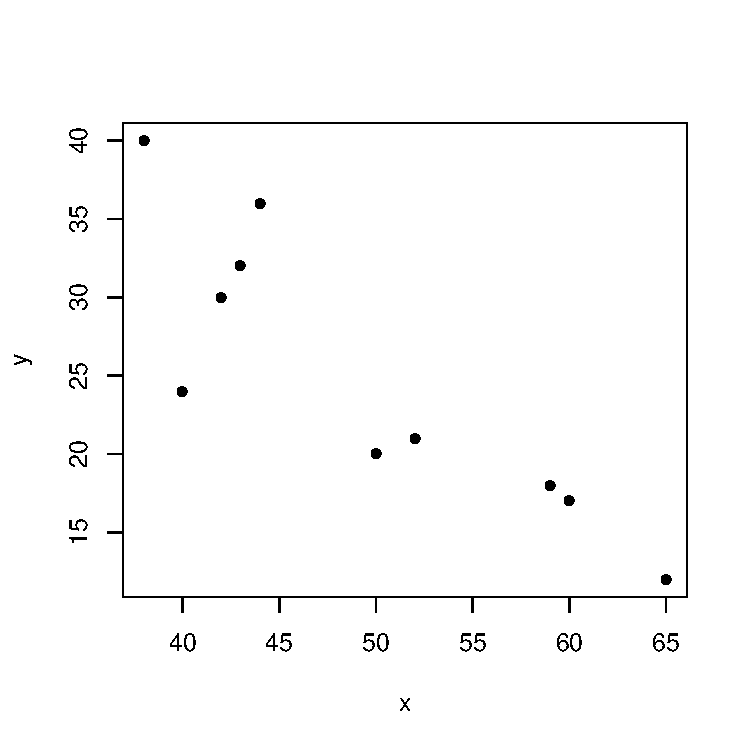
\includegraphics[width=.45\linewidth]{figure/fig-simple-base-1} 

}



\end{knitrout}
        \caption{Relation entre les données de l'exercice
          \ref{chap:simple}.\ref{ex:simple:base}}
        \label{fig:simple:base}
      \end{figure}
    \item Les équations normales sont les équations à résoudre pour
      trouver les estimateurs de $\beta_0$ et $\beta_1$ minimisant la
      somme des carrés
      \begin{align*}
        S(\beta_0, \beta_1)
        &=\sum_{i = 1}^n \varepsilon^2_i \\
        &=\sum_{i = 1}^n \left(Y_i-\beta_0-\beta_1x_i\right)^2.
      \end{align*}
      Or,
      \begin{align*}
        \frac{\partial S}{\partial \beta_0}
        &= -2 \sum_{i=1}^n (Y_i - \beta_0 - \beta_1 x_i) \\
        \frac{\partial S}{\partial \beta_1}
        &= -2 \sum_{i=1}^n (Y_i - \beta_0 - \beta_1 x_i) x_i,
      \end{align*}
      d'où les équations normales sont
      \begin{align*}
        \sum_{i=1}^n (Y_i - \hat{\beta}_0 - \hat{\beta}_1 x_i) &= 0 \\
        \sum_{i=1}^n (Y_i - \hat{\beta}_0 - \hat{\beta}_1 x_i) x_i &= 0.
      \end{align*}
    \item Par la première des deux équations normales, on trouve
      \begin{displaymath}
        \sum_{i=1}^nY_i-n\hat{\beta}_0-\hat{\beta}_1\sum_{i=1}^nx_i = 0,
      \end{displaymath}
      soit, en isolant $\hat{\beta}_0$,
      \begin{displaymath}
        \hat{\beta}_0=\frac{\sum_{i=1}^nY_i-\hat{\beta}_1\sum_{i=1}^nx_i}{n}=\bar{Y}-\hat{\beta}_1\bar{x}.
      \end{displaymath}
      De la seconde équation normale, on obtient
      \begin{displaymath}
        \sum_{i=1}^n x_i Y_i -
        \hat{\beta}_0 \sum_{i=1}^n x_i -
        \hat{\beta}_1 \sum_{i=1}^n x_i^2 = 0
      \end{displaymath}
      puis, en remplaçant $\hat{\beta}_0$ par la valeur obtenue ci-dessus,
      \begin{displaymath}
        \hat{\beta}_1
        \left(
          \sum_{i=1}^n x_i^2 - n \bar{x}^2
        \right) =
        \sum_{i=1}^n x_i Y_i - n \bar{x} \bar{Y}.
      \end{displaymath}
      Par conséquent,
      \begin{align*}
        \hat{\beta}_1
        &= \frac{\sum_{i=1}^n x_i Y_i - n \bar{x}\bar{Y}}{\sum_{i=1}^n
          x_i^2 - n \bar{x}^2} \\
        &= \frac{\nombre{11654} - (10)(49,3)(25)}{\nombre{25103} -
          (10)(49,3)^2} \\
        &= -0,8407 \\
        \intertext{et}
        \hat{\beta}_0
        &=\bar{Y}-\hat{\beta}_1\bar{x}\\
        &=25 - (-0,8407)(49,3)\\
        &=66,4488.
      \end{align*}
    \item On peut calculer les prévisions correspondant à $x_1, \dots,
      x_{10}$ --- ou valeurs ajustées --- à partir de la relation
      $\hat{Y}_i = 66,4488 - 0,8407 x_i$, $i = 1, 2, \dots, 10$. Avec
      \textsf{R}, on crée un objet de type modèle de régression avec
      \texttt{lm} et on en extrait les valeurs ajustées avec
      \texttt{fitted}:
\begin{knitrout}
\definecolor{shadecolor}{rgb}{0.969, 0.969, 0.969}\color{fgcolor}\begin{kframe}
\begin{alltt}
\hlstd{fit} \hlkwb{<-} \hlkwd{lm}\hlstd{(y} \hlopt{~} \hlstd{x)}
\hlkwd{fitted}\hlstd{(fit)}
\end{alltt}
\begin{verbatim}
##        1        2        3        4        5        6 
## 11.80028 30.29670 29.45596 16.84476 16.00401 24.41148 
##        7        8        9       10 
## 22.72998 34.50044 31.13745 32.81894
\end{verbatim}
\end{kframe}
\end{knitrout}
      Pour ajouter la droite de régression au graphique de la figure
      \ref{fig:simple:base}, il suffit d'utiliser la fonction
      \texttt{abline} avec en argument l'objet créé avec
      \texttt{lm}. L'ordonnée à l'origine et la pente de la droite
      seront extraites automatiquement. Voir la figure \ref{fig:simple:base2}.
      \begin{figure}
\begin{knitrout}
\definecolor{shadecolor}{rgb}{0.969, 0.969, 0.969}\color{fgcolor}\begin{kframe}
\begin{alltt}
\hlkwd{abline}\hlstd{(fit)}
\end{alltt}
\end{kframe}
\end{knitrout}
\begin{knitrout}
\definecolor{shadecolor}{rgb}{0.969, 0.969, 0.969}\color{fgcolor}

{\centering 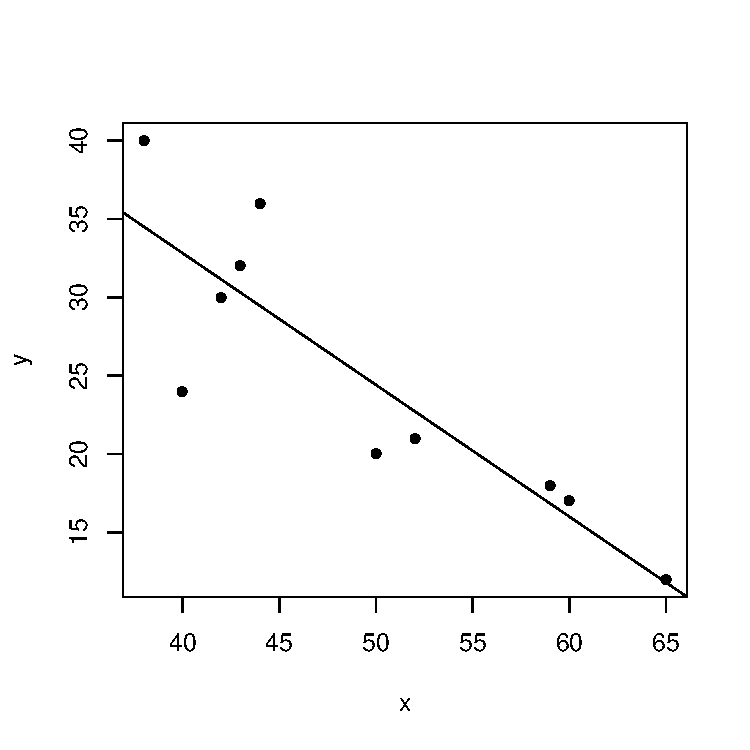
\includegraphics[width=.45\linewidth]{figure/fig-simple-base2-1} 

}



\end{knitrout}
        \caption{Relation entre les données de l'exercice
          \ref{chap:simple}.\ref{ex:simple:base} et la droite de
          régression}
        \label{fig:simple:base2}
      \end{figure}
    \item Les résidus de la régression sont $\varepsilon_i = Y_i - \hat{Y}_i$,
      $i = 1, \dots, 10$. Dans \textsf{R}, la fonction
      \texttt{residuals} extrait les résidus du modèle:
\begin{knitrout}
\definecolor{shadecolor}{rgb}{0.969, 0.969, 0.969}\color{fgcolor}\begin{kframe}
\begin{alltt}
\hlkwd{residuals}\hlstd{(fit)}
\end{alltt}
\begin{verbatim}
##          1          2          3          4          5 
##  0.1997243  1.7032953  6.5440421  1.1552437  0.9959905 
##          6          7          8          9         10 
## -4.4114773 -1.7299837  5.4995615 -1.1374514 -8.8189450
\end{verbatim}
\end{kframe}
\end{knitrout}
      On vérifie ensuite que la somme des résidus est
      (essentiellement) nulle:
\begin{knitrout}
\definecolor{shadecolor}{rgb}{0.969, 0.969, 0.969}\color{fgcolor}\begin{kframe}
\begin{alltt}
\hlkwd{sum}\hlstd{(}\hlkwd{residuals}\hlstd{(fit))}
\end{alltt}
\begin{verbatim}
## [1] -4.440892e-16
\end{verbatim}
\end{kframe}
\end{knitrout}
    \end{enumerate}
  \end{sol}
\end{exercice}

\begin{exercice}
  On vous donne les observations ci-dessous.
  \begin{center}
    \begin{minipage}[t]{0.3\textwidth}
      \mbox{} \\
      \begin{tabular}{ccc}
        \toprule
        $t$ & $x_i$ & $Y_i$ \\
        \midrule
        1 & 2 & 6 \\
        2 & 3 & 4 \\
        3 & 5 & 6 \\
        4 & 7 & 3 \\
        5 & 4 & 6 \\
        6 & 4 & 4 \\
        7 & 1 & 7 \\
        8 & 6 & 4 \\
        \bottomrule
      \end{tabular}
    \end{minipage}
    \begin{minipage}[t]{0.4\textwidth}
      \mbox{} \\[-1cm]
      \begin{align*}
        \sum_{i=1}^8 x_i &= 32 &
        \sum_{i=1}^8 x_i^2 &= 156 \\
        \sum_{i=1}^8 Y_i &= 40 &
        \sum_{i=1}^8 Y_i^2 &= 214 \\
        \sum_{i=1}^8 x_i\, Y_i &= 146 \\
      \end{align*}
    \end{minipage}
  \end{center}
  \begin{enumerate}
  \item Calculer les coefficients de la régression $Y_i = \beta_0 +
    \beta_1 x_i + \varepsilon_i$, $\var{\varepsilon_i} = \sigma^2$.
  \item Construire le tableau d'analyse de variance de la régression
    en a) et calculer le coefficient de détermination $R^2$.
    Interpréter les résultats.
  \end{enumerate}
  \begin{rep}
    \begin{inparaenum}
    \item $\hat{\beta}_0=7$ et $\hat{\beta}_1=-0,5$
    \item SST = 14, SSR = 7, SSE = 7, MSR = 7, MSE = 7/6, $F$ = 6, $R^2$ = 0,5
    \end{inparaenum}
  \end{rep}
  \begin{sol}
    \begin{enumerate}
    \item Nous avons le modèle de régression usuel. Les coefficients
      de la régression sont
      \begin{align*}
        \hat{\beta}_1
        &=\frac{\sum_{i=1}^8 x_iY_i-n\bar{x}\bar{Y}}{\sum_{i=1}^8
          x_i^2-n\bar{x}^2} \\
        &=\frac{146-(8)(32/8)(40/8)}{156-(8)(32/8)^2}  \\
        &=-0,5 \\
        \intertext{et}
        \hat{\beta}_0
        &=\bar{Y}-\hat{\beta}_1\bar{x} \\
        &=(40/8)-(-0,5)(32/8) \\
        &=7.
      \end{align*}
    \item Les sommes de carrés sont
      \begin{align*}
        \SST
        &=\sum_{i=1}^8(Y_i-\bar{Y})^2 \\
        &=\sum_{i=1}^8Y_i^2-n\bar{Y}^2 \\
        &=214-(8)(40/8)^2 \\
        &=14, \\
        \SSR
        &=\sum_{i=1}^8(\hat{Y}_i-\bar{Y})^2 \\
        &=\sum_{i=1}^8\hat{\beta}_1^2(x_i-\bar{x})^2 \\
        &=\hat{\beta}_1^2(\sum_{i=1}^8x_i^2-n\bar{x}^2) \\
        &=(-1/2)^2(156-(8)(32/8)^2) \\
        &=7.
      \end{align*}
      et $\SSE = \SST - \SSR = 14 - 7 = 7$. Par conséquent, $R^2 =
      SSR/SST = 7/14 = 0,5$, donc la régression explique 50~\% de la
      variation des $Y_i$ par rapport à leur moyenne $\bar{Y}$. Le
      tableau ANOVA est le suivant:
      \begin{center}
        \begin{tabular}{lcccc}
          \toprule
          Source & SS & d.l. & MS & Ratio F \\
          \midrule
          Régression & 7 & 1 & 7   & 6 \\
          Erreur     & 7 & 6 & 7/6 &  \\
          \midrule
          Total & 14 & 7 & & \\
          \bottomrule
        \end{tabular}
      \end{center}
    \end{enumerate}
  \end{sol}
\end{exercice}

\begin{exercice}
  Le jeu de données \texttt{women.dat}, disponible à l'URL mentionnée
  dans l'introduction et inclus dans \textsf{R}, contient les tailles
  et les poids moyens de femmes américaines âgées de 30 à 39 ans.
  Importer les données dans dans \textsf{R} ou rendre le jeu de
  données disponible avec \texttt{data(women)}, puis répondre aux
  questions suivantes.
  \begin{enumerate}
  \item Établir graphiquement une relation entre la taille
    (\emph{height}) et le poids (\emph{weight}) des femmes.
  \item À la lumière du graphique en a), proposer un modèle de
    régression approprié et en estimer les paramètres.
  \item Ajouter la droite de régression calculée en b) au
    graphique. Juger visuellement de l'ajustement du modèle.
  \item Obtenir, à l'aide de la fonction \texttt{summary} la valeur du
    coefficient de détermination $R^2$. La valeur est-elle conforme à
    la conclusion faite en c)?
  \item Calculer les statistiques $\SST$, $\SSR$ et
    $\SSE$, puis vérifier que $\SST = \SSR +
    \SSE$.  Calculer ensuite la valeur de $R^2$ et la comparer
    à celle obtenue en d).
  \end{enumerate}

  \begin{rep}
    \begin{inparaenum}
      \stepcounter{enumi}
    \item
      $\hat{\beta}_0 = -87,5167$
      et
      $\hat{\beta}_1 = 3,45$
      \stepcounter{enumi}
    \item $R^2 = 0,991$
    \item
      $\SSR = 3332,7$
      $\SSE = 30,23$ et
      $\SST = 3362,93$
    \end{inparaenum}
  \end{rep}
  \begin{sol}
    \begin{enumerate}
    \item Voir la figure \ref{fig:simple:women}.
      \begin{figure}
        \centering
\begin{knitrout}
\definecolor{shadecolor}{rgb}{0.969, 0.969, 0.969}\color{fgcolor}\begin{kframe}
\begin{alltt}
\hlkwd{data}\hlstd{(women)}
\hlkwd{plot}\hlstd{(weight} \hlopt{~} \hlstd{height,} \hlkwc{data} \hlstd{= women,} \hlkwc{pch} \hlstd{=} \hlnum{16}\hlstd{)}
\end{alltt}
\end{kframe}

{\centering 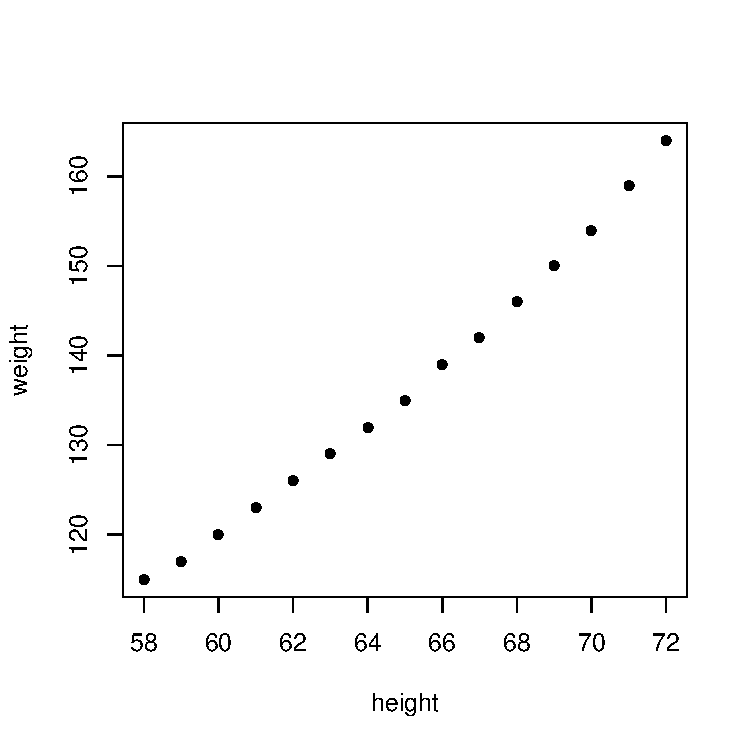
\includegraphics[width=.45\linewidth]{figure/fig-unnamed-chunk-8-1} 

}



\end{knitrout}
        \caption{Relation entre la taille et le poids moyen de femmes américaines âgées de 30 à 39 ans (données \texttt{women})}
        \label{fig:simple:women}
      \end{figure}
    \item Le graphique montre qu'un modèle linéaire serait
      excellent. On estime les paramètres de ce modèle avec \texttt{lm}:
\begin{knitrout}
\definecolor{shadecolor}{rgb}{0.969, 0.969, 0.969}\color{fgcolor}\begin{kframe}
\begin{alltt}
\hlstd{(fit} \hlkwb{<-} \hlkwd{lm}\hlstd{(weight} \hlopt{~} \hlstd{height,} \hlkwc{data} \hlstd{= women))}
\end{alltt}
\begin{verbatim}
## 
## Call:
## lm(formula = weight ~ height, data = women)
## 
## Coefficients:
## (Intercept)       height  
##      -87.52         3.45
\end{verbatim}
\end{kframe}
\end{knitrout}
    \item Voir la figure \ref{fig:simple:women2}.
      \begin{figure}
        \centering
\begin{knitrout}
\definecolor{shadecolor}{rgb}{0.969, 0.969, 0.969}\color{fgcolor}\begin{kframe}
\begin{alltt}
\hlkwd{abline}\hlstd{(fit)}
\end{alltt}
\end{kframe}
\end{knitrout}
\begin{knitrout}
\definecolor{shadecolor}{rgb}{0.969, 0.969, 0.969}\color{fgcolor}

{\centering 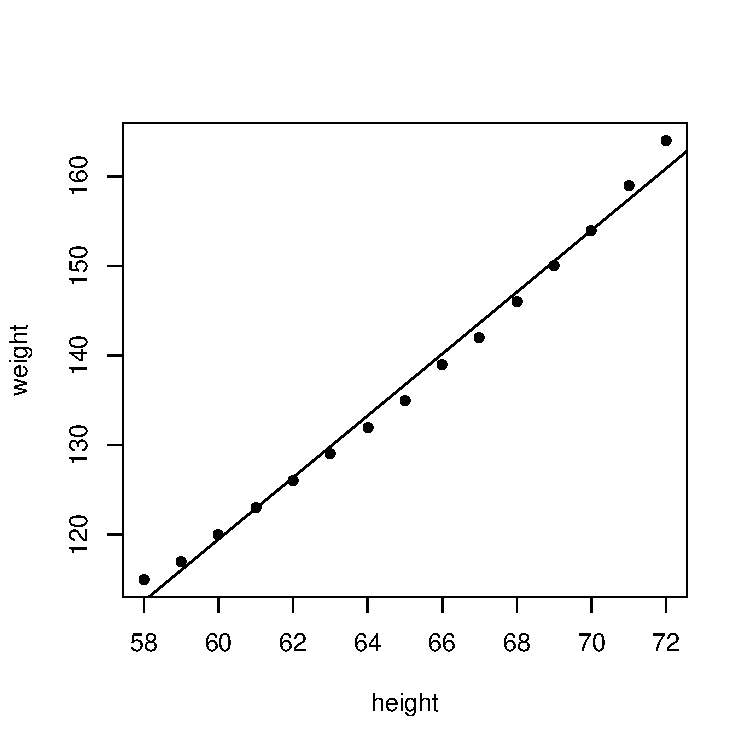
\includegraphics[width=.45\linewidth]{figure/fig-unnamed-chunk-11-1} 

}



\end{knitrout}
        \caption{Relation entre les données \texttt{women} et droite de régression linéaire simple}
        \label{fig:simple:women2}
      \end{figure}
      On constate que l'ajustement est excellent.
    \item Le résultat de la fonction \texttt{summary} appliquée au
      modèle \texttt{fit} est le suivant:
\begin{knitrout}
\definecolor{shadecolor}{rgb}{0.969, 0.969, 0.969}\color{fgcolor}\begin{kframe}
\begin{alltt}
\hlkwd{summary}\hlstd{(fit)}
\end{alltt}
\begin{verbatim}
## 
## Call:
## lm(formula = weight ~ height, data = women)
## 
## Residuals:
##     Min      1Q  Median      3Q     Max 
## -1.7333 -1.1333 -0.3833  0.7417  3.1167 
## 
## Coefficients:
##              Estimate Std. Error t value Pr(>|t|)    
## (Intercept) -87.51667    5.93694  -14.74 1.71e-09 ***
## height        3.45000    0.09114   37.85 1.09e-14 ***
## ---
## Signif. codes:  
## 0 '***' 0.001 '**' 0.01 '*' 0.05 '.' 0.1 ' ' 1
## 
## Residual standard error: 1.525 on 13 degrees of freedom
## Multiple R-squared:  0.991,	Adjusted R-squared:  0.9903 
## F-statistic:  1433 on 1 and 13 DF,  p-value: 1.091e-14
\end{verbatim}
\end{kframe}
\end{knitrout}
      Le coefficient de détermination est donc
      $R^2 = 0,991$, %$
      ce qui est près de 1 et confirme donc l'excellent
      ajustement du modèle évoqué en c).
    \item On a
\begin{knitrout}
\definecolor{shadecolor}{rgb}{0.969, 0.969, 0.969}\color{fgcolor}\begin{kframe}
\begin{alltt}
\hlkwd{attach}\hlstd{(women)}
\hlstd{SST} \hlkwb{<-} \hlkwd{sum}\hlstd{((weight} \hlopt{-} \hlkwd{mean}\hlstd{(weight))}\hlopt{^}\hlnum{2}\hlstd{)}
\hlstd{SSR} \hlkwb{<-} \hlkwd{sum}\hlstd{((}\hlkwd{fitted}\hlstd{(fit)} \hlopt{-} \hlkwd{mean}\hlstd{(weight))}\hlopt{^}\hlnum{2}\hlstd{)}
\hlstd{SSE} \hlkwb{<-} \hlkwd{sum}\hlstd{((weight} \hlopt{-} \hlkwd{fitted}\hlstd{(fit))}\hlopt{^}\hlnum{2}\hlstd{)}
\hlkwd{all.equal}\hlstd{(SST, SSR} \hlopt{+} \hlstd{SSE)}
\end{alltt}
\begin{verbatim}
## [1] TRUE
\end{verbatim}
\begin{alltt}
\hlkwd{all.equal}\hlstd{(}\hlkwd{summary}\hlstd{(fit)}\hlopt{$}\hlstd{r.squared, SSR}\hlopt{/}\hlstd{SST)}
\end{alltt}
\begin{verbatim}
## [1] TRUE
\end{verbatim}
\end{kframe}
\end{knitrout}
    \end{enumerate}
  \end{sol}
\end{exercice}

\begin{exercice}
  Dans le contexte de la régression linéaire simple, démontrer que
  \begin{displaymath}
    \sum_{i=1}^n (\hat{Y}_i - \bar{Y}) \varepsilon_i = 0.
  \end{displaymath}
  \begin{sol}
    Puisque $\hat{Y}_i = (\bar{Y} - \hat{\beta}_1 \bar{x}) +
    \hat{\beta}_1 x_i = \bar{Y} + \hat{\beta}_1 (x_i - \bar{x})$ et
    que $\varepsilon_i = Y_i - \hat{Y}_i = (Y_i - \bar{Y}) - \hat{\beta}_1 (x_i
    - \bar{x})$, alors
    \begin{align*}
      \sum_{i = 1}^n (\hat{Y}_i - \bar{Y}) \varepsilon_i
      &= \hat{\beta}_1
      \left(
        \sum_{i=1}^n (x_i - \bar{x})(Y_i - \bar{Y}) -
        \hat{\beta}_1 \sum_{i = 1}^n (x_i - \bar{x})^2
      \right) \\
      & = \hat{\beta}_1
      \left(
        S_{xy} - \frac{S_{xy}}{S_{xx}}\, S_{xx}
      \right) \\
      & = 0.
    \end{align*}
  \end{sol}
\end{exercice}

\begin{exercice}
  Considérer le modèle de régression linéaire par rapport au temps
  $Y_t = \beta_0 + \beta_1 t + \varepsilon_t$, $t = 1, \dots, n$. Écrire
  les équations normales et obtenir les estimateurs des moindres
  carrés des paramètres $\beta_0$ et $\beta_1$. \emph{Note}:
  $\sum_{i=1}^n i^2 = n(n + 1)(2n + 1)/6$.
  \begin{rep}
    $\hat{\beta}_0 = \bar{Y} - \hat{\beta}_1 (n + 1)/2$,
    $\hat{\beta}_1 = (12 \sum_{t = 0}^n t Y_t - 6 n (n + 1)
    \bar{Y})/(n (n^2 - 1)$
  \end{rep}
  \begin{sol}
    On a un modèle de régression linéaire simple usuel avec $x_t =
    t$. Les estimateurs des moindres carrés des paramètres $\beta_0$ et
    $\beta_1$ sont donc
    \begin{align*}
      \hat{\beta}_0
      &= \bar{Y} - \hat{\beta}_1\, \frac{\sum_{t = 1}^n t}{n} \\
      \intertext{et}
      \hat{\beta}_1
      &= \frac{\sum_{t = 1}^n t Y_t - \bar{Y} \sum_{t = 1}^n t}{\sum_{t
          = 1}^n t^2 - n^{-1} (\sum_{t = 1}^n t)^2}.
    \end{align*}
    Or, puisque $\sum_{t = 1}^n t = n(n + 1)/2$ et $\sum_{t = 1}^n t^2
    = n(n + 1)(2n + 1)/6$, les expressions ci-dessus se simplifient en
    \begin{align*}
      \hat{\beta}_0
      & = \bar{Y} - \hat{\beta}_1\, \frac{n + 1}{2} \\
      \intertext{et}
      \hat{\beta}_1
      & = \frac{\sum_{t=1}^n t Y_t - n(n + 1) \bar{Y}/2}{n(n + 1)(2n +
        1)/6 - n(n + 1)^2/4} \\
      & = \frac{12 \sum_{t=1}^n t Y_t - 6 n (n + 1) \bar{Y}}{n (n^2 - 1)}.
    \end{align*}
  \end{sol}
\end{exercice}

\begin{exercice}
  \label{ex:simple:origine}
  \begin{enumerate}
  \item Trouver l'estimateur des moindres carrés du paramètre $\beta$
    dans le modèle de régression linéaire passant par l'origine $Y_i =
    \beta x_i + \varepsilon_i$, $i = 1, \dots, n$,
    $\esp{\varepsilon_i} = 0$, $\Cov(\varepsilon_i, \varepsilon_j) =
    \delta_{ij} \sigma^2$.
  \item Démontrer que l'estimateur en a) est sans biais.
  \item Calculer la variance de l'estimateur en a).
  \end{enumerate}
  \begin{rep}
    \begin{inparaenum}
    \item $\hat{\beta}= \sum_{i = 1}^n x_i Y_i/\sum_{i = 1}^n x_i^2$
      \stepcounter{enumi}
    \item $\var{\hat{\beta}} = \sigma^2/\sum_{i = 1}^n x_i^2$
    \end{inparaenum}
  \end{rep}
  \begin{sol}
    \begin{enumerate}
    \item L'estimateur des moindres carrés du paramètre $\beta$ est la
      valeur $\hat{\beta}$ minimisant la somme de carrés
      \begin{align*}
        S(\beta)
        &=\sum_{i = 1}^n \varepsilon_i^2 \\
        &=\sum_{i = 1}^n (Y_i - \beta x_i)^2.
      \end{align*}
      Or,
      \begin{displaymath}
        \frac{d}{d \beta}\, S(\beta) = -2 \sum_{i = 1}^n (Y_i -
        \hat{\beta} x_i) x_i,
      \end{displaymath}
      d'où l'unique équation normale de ce modèle est
      \begin{displaymath}
        \sum_{i = 1}^n x_i Y_i - \hat{\beta} \sum_{i=1}^n x_i^2 = 0.
      \end{displaymath}
      L'estimateur des moindres carrés de $\beta$ est donc
      \begin{displaymath}
        \hat{\beta} = \frac{\sum_{i=1}^n x_i Y_i}{\sum_{i=1}^n x_i^2}.
      \end{displaymath}
    \item On doit démontrer que $\esp{\hat{\beta}} = \beta$. On a
      \begin{align*}
        \esp{\hat{\beta}}
        &= \Esp{\frac{\sum_{i=1}^n x_i Y_i}{\sum_{i=1}^n x_i^2}} \\
        &= \frac{1}{\sum_{i=1}^n x_i^2} \sum_{i=1}^n x_i \esp{Y_i} \\
        &= \frac{1}{\sum_{i=1}^nx_i^2} \sum_{i=1}^n x_i \beta x_i \\
        &= \beta\, \frac{\sum_{i=1}^n x_i^2}{\sum_{i=1}^n x_i^2} \\
        &= \beta.
      \end{align*}
    \item Des hypothèses du modèle, on a
      \begin{align*}
        \var{\hat{\beta}}
        &= \Var{\frac{\sum_{i=1}^n x_i Y_i}{\sum_{i=1}^n x_i^2}} \\
        &= \frac{1}{(\sum_{i=1}^n x_i^2)^2} \sum_{i=1}^n x_i^2 \var{Y_i} \\
        &= \frac{\sigma^2}{(\sum_{i=1}^n x_i^2)^2} \sum_{i=1}^n x_i^2 \\
        &= \frac{\sigma^2}{\sum_{i=1}^n x_i^2}.
      \end{align*}
    \end{enumerate}
  \end{sol}
\end{exercice}

\begin{exercice}
  Démontrer que l'estimateur des moindres carrés $\hat{\beta}$ trouvé à
  l'exercice \ref{chap:simple}.\ref{ex:simple:origine} est
  l'estimateur sans biais à variance (uniformément) minimale du
  paramètre $\beta$.  En termes mathématiques: soit
  \begin{displaymath}
    \beta^* = \sum_{i=1}^n c_i Y_i
  \end{displaymath}
  un estimateur linéaire du paramètre $\beta$. Démontrer qu'en
  déterminant les coefficients $c_1, \dots, c_n$ de façon à minimiser
  \begin{displaymath}
    \var{\beta^*} = \Var{\sum_{i=1}^n c_i Y_i}
  \end{displaymath}
  sous la contrainte que
  \begin{displaymath}
    \esp{\beta^*} = \Esp{\sum_{i=1}^n c_i Y_i} = \beta,
  \end{displaymath}
  on obtient $\beta^* = \hat{\beta}$.
  \begin{sol}
    On veut trouver les coefficients $c_1, \dots, c_n$ tels que
    $\esp{\beta^*} = \beta$ et $\var{\beta^*}$ est minimale. On
    cherche donc à minimiser la fonction
    \begin{align*}
      f(c_1, \dots, c_n)
      &= \var{\beta^*} \\
      &= \sum_{i=1}^n c_i^2 \var{Y_i} \\
      &= \sigma^2 \sum_{i=1}^n c_i^2
    \end{align*}
    sous la contrainte $\esp{\beta^*} = \sum_{i=1}^nc_i\esp{Y_i} =
    \sum_{i=1}^nc_i\beta x_i = \beta\sum_{i=1}^nc_ix_i = \beta$, soit
    $\sum_{i=1}^n c_i x_i = 1$ ou $g(c_1, \dots, c_n) = 0$ avec
    \begin{displaymath}
      g(c_1, \dots, c_n) = \sum_{i=1}^n c_i x_i - 1.
    \end{displaymath}
    Pour utiliser la méthode des multiplicateurs de Lagrange, on pose
    \begin{align*}
      \mathcal{L}(c_1, \dots, c_n,\lambda)
      &= f(c_1, \dots, c_n) - \lambda g(c_1, \dots, c_n), \\
      &= \sigma^2 \sum_{i=1}^n c_i^2 - \lambda
      \left(
        \sum_{i=1}^n c_i x_i - 1
      \right),
    \end{align*}
    puis on dérive la fonction $\mathcal{L}$ par rapport à chacune des
    variables $c_1, \dots, c_n$ et $\lambda$. On trouve alors
    \begin{align*}
      \frac{\partial \mathcal{L}}{\partial c_u}
      & = 2 \sigma^2 c_u - \lambda x_u, \quad u = 1, \dots, n \\
      \frac{\partial \mathcal{L}}{\partial \lambda}
      & = - \sum_{i=1}^n c_i x_i + 1.
    \end{align*}
    En posant les $n$ premières dérivées égales à zéro, on obtient
    \begin{displaymath}
      c_i = \frac{\lambda x_i}{2 \sigma^2}.
    \end{displaymath}
    Or, de la contrainte,
    \begin{displaymath}
      \sum_{i=1}^n c_i x_i =
      \frac{\lambda}{2\sigma^2} \sum_{i=1}^n x_i^2 = 1,
    \end{displaymath}
    d'où
    \begin{displaymath}
      \frac{\lambda}{2 \sigma^2} = \frac{1}{\sum_{i=1}^n x_i^2}
    \end{displaymath}
    et, donc,
    \begin{displaymath}
      c_i = \frac{x_i}{\sum_{i=1}^n x_i^2}.
    \end{displaymath}
    Finalement,
    \begin{align*}
      \beta^*
      & = \sum_{i=1}^n c_i Y_i \\
      & = \frac{\sum_{i=1}^n x_i Y_i}{\sum_{i=1}^n x_i^2} \\
      & = \hat{\beta}.
    \end{align*}
  \end{sol}
\end{exercice}

\begin{exercice}
  Dans le contexte de la régression linéaire simple, démontrer que
  \begin{enumerate}
  \item $\esp{\MSE} = \sigma^2$
  \item $\esp{\MSR} = \sigma^2 + \beta_1^2 \sum_{i=1}^n (x_i -
    \bar{x})^2$
  \end{enumerate}
  \begin{sol}
    \begin{enumerate}
    \item Tout d'abord, puisque $\MSE = \SSE/(n - 2) = \sum_{i=1}^n
      (Y_i - \hat{Y}_i)^2/(n - 2)$ et que $\esp{Y_i} =
      \esp{\hat{Y}_i}$, alors
      \begin{align*}
        \esp{MSE}
        &= \frac{1}{n - 2} \Esp{\sum_{i=1}^n (Y_i - \hat{Y}_i)^2} \\
        &= \frac{1}{n - 2} \sum_{i=1}^n \esp{(Y_i - \hat{Y}_i)^2} \\
        &= \frac{1}{n - 2} \sum_{i=1}^n \esp{((Y_i - \esp{Y_i}) -
          (\hat{Y}_i - \esp{\hat{Y}_i}))^2} \\
        &= \frac{1}{n - 2} \sum_{i=1}^n
        \left(
          \var{Y_i} + \var{\hat{Y}_i} - 2\, \Cov(Y_i, \hat{Y}_i)
        \right).
      \end{align*}
      Or, on a par hypothèse du modèle que $\Cov(Y_i, Y_j) =
      \Cov(\varepsilon_i, \varepsilon_j) = \delta_{ij} \sigma^2$, d'où
      $\var{Y_i} = \sigma^2$ et $\var{\bar{Y}} = \sigma^2/n$. D'autre
      part,
      \begin{align*}
        \var{\hat{Y}_i}
        &= \var{\bar{Y} + \hat{\beta}_1 (x_i - \bar{x})} \\
        &= \var{\bar{Y}} + (x_i - \bar{x})^2 \var{\hat{\beta}_1} +
        2 (x_i - \bar{x}) \Cov(\bar{Y}, \hat{\beta}_1)
      \end{align*}
      et l'on sait que
      \begin{align*}
        \var{\hat{\beta}_1}
        &= \frac{\sigma^2}{\sum_{i=1}^n(x_i-\bar{x})^2} \\
        \intertext{et que}
        \Cov(\bar{Y}, \hat{\beta}_1)
        & = \Cov
        \left(
          \frac{\sum_{i = 1}^n Y_i}{n},
          \frac{\sum_{j = 1}^n (x_j - \bar{x}) Y_j}{\sum_{j = 1}^n
            (x_j - \bar{x})^2}
        \right) \\
        &= \frac{1}{n \sum_{j = 1}^n (x_j - \bar{x})^2}
        \sum_{i = 1}^n \sum_{j = 1}^n \Cov(Y_i, (x_j - \bar{x}) Y_j) \\
        &= \frac{1}{n \sum_{j = 1}^n (x_j - \bar{x})^2}
        \sum_{i = 1}^n (x_j - \bar{x}) \var{Y_i} \\
        & = \frac{\sigma^2}{n \sum_{j = 1}^n (x_j - \bar{x})^2}
        \sum_{i = 1}^n (x_i - \bar{x}) \\
        & = 0,
      \end{align*}
      puisque $\sum_{i=1}^n(x_i - \bar{x}) = 0$. Ainsi,
      \begin{displaymath}
        \var{\hat{Y}_i} = \frac{\sigma^2}{n} +
        \frac{(x_i - \bar{x})^2 \sigma^2}{\sum_{i=1}^n (x_i - \bar{x})^2}.
      \end{displaymath}
      De manière similaire, on détermine que
      \begin{align*}
        \Cov(Y_i, \hat{Y}_i)
        &= \Cov(Y_i, \bar{Y} + \hat{\beta}_1 (x_i - \bar{x})) \\
        &= \Cov(Y_i, \bar{Y}) +
        (x_i - \bar{x}) \Cov(Y_i, \hat{\beta}_1) \\
        &= \frac{\sigma^2}{n} + \frac{(x_i -
          \bar{x})^2 \sigma^2}{\sum_{i=1}^n (x_i - \bar{x})^2}.
      \end{align*}
      Par conséquent,
      \begin{align*}
        \esp{(Y_i - \hat{Y}_i)^2}
        &= \frac{n - 1}{n}\, \sigma^2 -
        \frac{(x_i - \bar{x})^2 \sigma^2}{\sum_{i = 1}^n (x_i - \bar{x})^2} \\
        \intertext{et}
        \sum_{i=1}^n \esp{(Y_i - \hat{Y}_i)^2}
        & = (n - 2) \sigma^2,
      \end{align*}
      d'où $\esp{\MSE} = \sigma^2$.
    \item On a
      \begin{align*}
        \esp{\MSR}
        &= \esp{\SSR} \\
        &= \Esp{\sum_{i=1}^n (\hat{Y}_i - \bar{Y})^2} \\
        &= \sum_{i=1}^n \esp{\hat{\beta}_1^2 (x_i - \bar{x})^2} \\
        &= \sum_{i=1}^n (x_i - \bar{x})^2 \esp{\hat{\beta}_1^2} \\
        &= \sum_{i=1}^n (x_i - \bar{x})^2 (\var{\hat{\beta}_1} +
        \esp{\hat{\beta}_1}^2) \\
        &= \sum_{i=1}^n (x_i - \bar{x})^2
        \left(
          \frac{\sigma^2}{\sum_{i=1}^n (x_i - \bar{x})^2} + \beta_1^2
        \right) \\
        &= \sigma^2 + \beta_1^2 \sum_{i=1}^n (x_i - \bar{x})^2.
      \end{align*}
    \end{enumerate}
  \end{sol}
\end{exercice}

\begin{exercice}
  Supposons que les observations $(x_1, Y_1), \dots, (x_n, Y_n)$
  sont soumises à une transformation linéaire, c'est-à-dire que $Y_i$
  devient $Y_i^\prime = a + b Y_i$ et que $x_i$ devient $x_i^\prime =
  c + d x_i$, $i = 1, \dots, n$.
  \begin{enumerate}
  \item Trouver quel sera l'impact sur les estimateurs des moindres
    carrés des paramètres $\beta_0$ et $\beta_1$ dans le modèle de
    régression linéaire $Y_i = \beta_0 + \beta_1 x_i + \varepsilon_i$.
  \item Démontrer que le coefficient de détermination $R^2$ n'est pas
    affecté par la transformation linéaire.
  \end{enumerate}
  \begin{rep}
    \begin{enumerate}
    \item $\hat{\beta}_1^\prime = (b/d) \hat{\beta}_1$
    \end{enumerate}
  \end{rep}
  \begin{sol}
    \begin{enumerate}
    \item Il faut exprimer $\hat{\beta}_0^\prime$ et
      $\hat{\beta}_1^\prime$ en fonction de $\hat{\beta}_0$ et
      $\hat{\beta}_1$. Pour ce faire, on trouve d'abord une expression
      pour chacun des éléments qui entrent dans la définition de
      $\hat{\beta}_1^\prime$. Tout d'abord,
      \begin{align*}
        \bar{x}^\prime
        &= \frac{1}{n} \sum_{i=1}^n x_i^\prime \\
        &= \frac{1}{n} \sum_{i=1}^n (c + d x_i) \\
        &= c + d \bar{x},
      \end{align*}
      et, de manière similaire, $\bar{Y}^\prime = a + b \bar{Y}$. Ensuite,
      \begin{align*}
        S_{xx}^\prime
        &= \sum_{i=1}^n (x_i^\prime - \bar{x}^\prime)^2 \\
        &= \sum_{i=1}^n (c + d x_i - c - d \bar{x})^2 \\
        &= d^2 S_{xx}
      \end{align*}
      et $S_{yy}^\prime = b^2 S_{yy}$, $S_{xy}^\prime = bd S_{xy}$.
      Par conséquent,
      \begin{align*}
        \hat{\beta}_1^\prime
        &= \frac{S_{xy}^\prime}{S_{xx}^\prime} \\
        &= \frac{bd S_{xy}}{d^2 S_{xx}} \\
        &= \frac{b}{d}\, \hat{\beta}_1 \\
        \intertext{et}
        \hat{\beta}_0^\prime
        &= \bar{Y}^\prime - \hat{\beta}_1^\prime \bar{x}^\prime \\
        &= a + b \bar{Y} - \frac{b}{d}\, \hat{\beta}_1 (c + d \bar{x}) \\
        &= a - \frac{bc}{d}\, \hat{\beta}_1 + b (\bar{Y} -
        \hat{\beta}_1 \bar{x}) \\
        &= a - \frac{bc}{d}\, \hat{\beta}_1 + b \hat{\beta}_0.
      \end{align*}
    \item Tout d'abord, on établit que
      \begin{align*}
        R^2
        &= \frac{\SSR}{\SST} \\
        &= \frac{\sum_{i=1}^n (\hat{Y_i} - \bar{Y})^2}{\sum_{i=1}^n
          (Y_i - \bar{Y})^2} \\
        &= \hat{\beta}_1^2\, \frac{\sum_{i=1}^n (x_i -
          \bar{x})^2}{\sum_{i=1}^n (Y_i - \bar{Y})^2} \\
        &= \hat{\beta}_1^2\, \frac{S_{xx}}{S_{yy}}.
      \end{align*}
      Maintenant, avec les résultats obtenus en a), on démontre
      directement que
      \begin{align*}
        (R^2)^\prime
        &= (\hat{\beta}_1^\prime)^2 \frac{S_{xx}^\prime}{S_{yy}^\prime} \\
        &=
        \left(
          \frac{b}{d}
        \right)^2\,
        \hat{\beta}_1^2\, \frac{d^2 S_{xx}}{b^2 S_{yy}} \\
        &= \hat{\beta}_1^2\, \frac{S_{xx}}{S_{yy}} \\
        &= R^2.
      \end{align*}
    \end{enumerate}
  \end{sol}
\end{exercice}

\begin{exercice}
  On sait depuis l'exercice \ref{chap:simple}.\ref{ex:simple:origine}
  que pour le modèle de régression linéaire simple passant par
  l'origine $Y_i = \beta x_i + \varepsilon_i$, l'estimateur des
  moindres carrés de $\beta$ est
  \begin{displaymath}
    \hat{\beta} = \frac{\sum_{i = 1}^n x_i Y_i}{\sum_{i = 1}^n x_i^2}.
  \end{displaymath}
  Démontrer que l'on peut obtenir ce résultat en utilisant la formule
  pour $\hat{\beta}_1$ dans la régression linéaire simple usuelle
  ($Y_i = \beta_0 + \beta_1 x_i + \varepsilon_i$) en ayant d'abord
  soin d'ajouter aux données un $(n + 1)${\ieme} point $(m\bar{x},
  m\bar{Y})$, où
  \begin{displaymath}
    m = \frac{n}{\sqrt{n + 1} - 1} = \frac{n}{a}.
  \end{displaymath}
  \begin{sol}
    Considérons un modèle de régression usuel avec l'ensemble de
    données $(x_1, Y_1), \dots, (x_n, Y_n), (m \bar{x}, m \bar{Y})$,
    où $\bar{x} = n^{-1} \sum_{i = 1}^n x_i$, $\bar{Y} = n^{-1}
    \sum_{i = 1}^n Y_i$, $m = n/a$ et $a = \sqrt{n + 1} - 1$. On
    définit
    \begin{align*}
      \bar{x}^\prime
      &= \frac{1}{n + 1} \sum_{i = 1}^{n + 1} x_i \\
      &= \frac{1}{n + 1} \sum_{i = 1}^n x_i + \frac{m}{n + 1} \bar{x} \\
      &= k \bar{x} \\
      \intertext{et, de manière similaire,}
      \bar{Y}^\prime
      &= k \bar{Y},
      \intertext{où}
      k
      &= \frac{n + m}{n + 1} \\
      &= \frac{n (a + 1)}{a (n + 1)}.
    \end{align*}
    L'expression pour l'estimateur des moindres carrés de la pente de
    la droite de régression pour cet ensemble de données est
    \begin{align*}
      \hat{\beta}_1
      &= \frac{\sum_{i = 1}^{n + 1} x_i Y_i - (n + 1)
        \bar{x}^\prime \bar{Y}^\prime}{%
        \sum_{i = 1}^{n + 1} x_i^2 - (n + 1) (\bar{x}^\prime)^2} \\
      &= \frac{\sum_{i = 1}^n x_i Y_i + m^2 \bar{x} \bar{Y} - (n + 1)
        k^2 \bar{x} \bar{Y}}{%
        \sum_{i = 1}^n x_i^2 + m^2 \bar{x}^2 - (n + 1) k^2 \bar{x}^2}.
    \end{align*}
    Or,
    \begin{align*}
      m^2 - k^2 (n + 1)
      &= \frac{n^2}{a^2} - \frac{n^2 (a + 1)^2}{a^2 (n + 1)} \\
      &= \frac{n^2 (n + 1) - n^2 (n + 1)}{a^2 (n + 1)} \\
      &= 0.
    \end{align*}
    Par conséquent,
    \begin{align*}
      \hat{\beta}_1
      &= \frac{\sum_{i = 1}^n x_i Y_i}{\sum_{i = 1}^n x_i^2} \\
      &= \hat{\beta}.
    \end{align*}
    Interprétation: en ajoutant un point bien spécifique à n'importe
    quel ensemble de données, on peut s'assurer que la pente de la
    droite de régression sera la même que celle d'un modèle passant
    par l'origine. Voir la figure \ref{fig:simple:pointmagique} pour
    une illustration du phénomène.

    \begin{figure}
\begin{knitrout}
\definecolor{shadecolor}{rgb}{0.969, 0.969, 0.969}\color{fgcolor}

{\centering 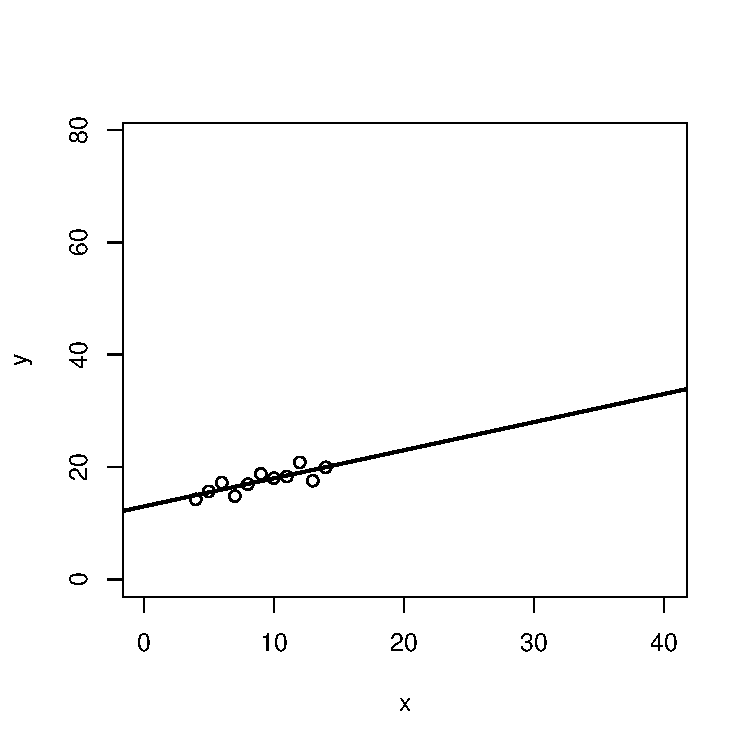
\includegraphics[width=.45\linewidth]{figure/fig-simple-pointmagique-1} 
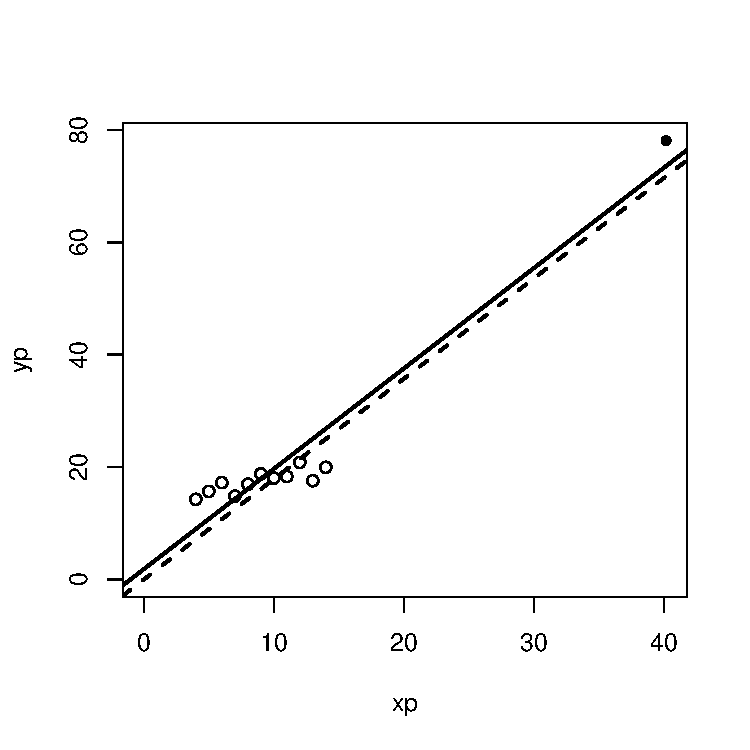
\includegraphics[width=.45\linewidth]{figure/fig-simple-pointmagique-2} 

}



\end{knitrout}
      \caption{Illustration de l'effet de l'ajout d'un point spécial à
        un ensemble de données. À gauche, la droite de régression
        usuelle. À droite, le même ensemble de points avec le point
        spécial ajouté (cercle plein), la droite de régression avec ce
        nouveau point (ligne pleine) et la droite de régression
        passant par l'origine (ligne pointillée). Les deux droites
        sont parallèles.}
      \label{fig:simple:pointmagique}
    \end{figure}
  \end{sol}
\end{exercice}

\begin{exercice}
  Soit le modèle de régression linéaire simple
  \begin{displaymath}
    Y_i = \beta_0 + \beta_1 x_i + \varepsilon_i, \quad
    \varepsilon_i \sim N(0, \sigma^2).
  \end{displaymath}
  Construire un intervalle de confiance de niveau $1 - \alpha$ pour le
  paramètre $\beta_1$ si la variance $\sigma^2$ est connue.
  \begin{rep}
    $\beta_1 \in \hat{\beta}_1 \pm z_{\alpha/2} \sigma
    \left( \sum_{i=1}^n (x_i - \bar{x})^2 \right)^{-1/2}$
  \end{rep}
  \begin{sol}
    Puisque, selon le modèle, $\varepsilon_i \sim N(0, \sigma^2)$ et
    que $Y_i = \beta_0 + \beta_1 x_i + \varepsilon_i$, alors $Y_i \sim
    N(\beta_0 + \beta_1 x_i, \sigma^2)$. De plus, on sait que
    \begin{align*}
      \hat{\beta}_1
      &= \frac{\sum_{i=1}^n (x_i - \bar{x})(Y_i - \bar{Y})}{%
        \sum_{i=1}^n (x_i - \bar{x})^2} \\
      &= \frac{\sum_{i=1}^n (x_i - \bar{x}) Y_i}{%
        \sum_{i=1}^n (x_i - \bar{x})^2},
    \end{align*}
    donc l'estimateur $\hat{\beta}_1$ est une combinaison linéaire des
    variables aléatoires $Y_1, \dots, Y_n$. Par conséquent,
    $\hat{\beta}_1 \sim N(\esp{\hat{\beta}_1}, \var{\hat{\beta}_1})$,
    où $\esp{\hat{\beta}_1} = \beta_1$ et $\var{\hat{\beta}_1} =
    \sigma^2/S_{xx}$ et, donc,
    \begin{displaymath}
      \Pr
      \left[
        -z_{\alpha/2} <
        \frac{\hat{\beta}_1 - \beta_1}{\sigma/\sqrt{S_{xx}}} <
        z_{\alpha/2}
      \right] = 1 - \alpha.
    \end{displaymath}
    Un intervalle de confiance de niveau $1 - \alpha$ pour le
    paramètre $\beta_1$ lorsque la variance $\sigma^2$ est connue est donc
    \begin{displaymath}
      \beta_1 \in \hat{\beta}_1 \pm z_{\alpha/2}
      \frac{\sigma}{\sqrt{\sum_{i=1}^n (x_i - \bar{x})^2}}.
    \end{displaymath}
  \end{sol}
\end{exercice}

\begin{exercice}
  Vous analysez la relation entre la consommation de gaz naturel
  \emph{per capita} et le prix du gaz naturel. Vous avez colligé les
  données de 20 grandes villes et proposé le modèle
  \begin{displaymath}
    Y = \beta_0 + \beta_1 x + \varepsilon,
  \end{displaymath}
  où $Y$ représente la consommation de gaz \emph{per capita}, $x$ le
  prix et $\varepsilon$ est le terme d'erreur aléatoire distribué
  selon une loi normale. Vous avez obtenu les résultats suivants:
  \begin{align*}
    \hat{\beta}_0 &= 138,581 &
      \sum_{i=1}^{20} (x_i - \bar{x})^2 &= \nombre{10668} \\
    \hat{\beta}_1 &= -1,104 &
      \sum_{i=1}^{20} (Y_i - \bar{Y})^2 &= \nombre{20838} \\
    \sum_{i=1}^{20} x_i^2 &= \nombre{90048} &
      \sum_{i=1}^{20} \varepsilon_i^2 &= \nombre{7832}. \\
    \sum_{i=1}^{20} Y_i^2 &= \nombre{116058}
  \end{align*}
  Trouver le plus petit intervalle de confiance à 95~\% pour le
  paramètre $\beta_1$.
  \begin{rep}
    $(-1,5, -0,7)$
  \end{rep}
  \begin{sol}
    L'intervalle de confiance pour $\beta_1$ est
    \begin{align*}
      \beta_1
      &\in \hat{\beta}_1 \pm t_{\alpha/2}(n - 2)
      \sqrt{\frac{\hat{\sigma}^2}{S_{xx}}} \\
      &\in \hat{\beta}_1 \pm t_{0,025}(20 - 2) \sqrt{\frac{MSE}{S_{xx}}}.
     \end{align*}
     On nous donne $\SST = S_{yy} = \nombre{20838}$ et $S_{xx} =
     \nombre{10668}$. Par conséquent,
     \begin{align*}
       \SSR
       &= \hat{\beta}_1^2 \sum_{i=1}^{20} (x_i - \bar{x})^2 \\
       &= (-1,104)^2(\nombre{10668}) \\
       &= \nombre{13002,33} \\
       \SSE
       &= \SST - \SSR \\
       &= \nombre{7835,67} \\
       \intertext{et}
       \MSE
       &= \frac{\SSE}{18} \\
       &= 435,315.
     \end{align*}
     De plus, on trouve dans une table de quantiles de la loi de
     Student (ou à l'aide de la fonction \texttt{qt} dans \textsf{R})
     que $t_{0,025}(18) = 2,101$. L'intervalle de confiance recherché
     est donc
     \begin{align*}
       \beta_1
       &\in -1,104 \pm 2,101 \sqrt{\frac{435,315}{\nombre{10668}}} \\
       &\in (-1,528, -0,680).
     \end{align*}
  \end{sol}
\end{exercice}

\begin{exercice}
  Le tableau ci-dessous présente les résultats de l'effet de la
  température sur le rendement d'un procédé chimique.
  \begin{center}
    \begin{tabular}{rr}
      \toprule
      $x$ & $Y$ \\
      \midrule
      $-5$ &  1 \\
      $-4$ &  5 \\
      $-3$ &  4 \\
      $-2$ &  7 \\
      $-1$ & 10 \\
        0  &  8 \\
        1  &  9 \\
        2  & 13 \\
        3  & 14 \\
        4  & 13 \\
        5  & 18 \\
      \bottomrule
    \end{tabular}
  \end{center}
  \begin{enumerate}
  \item On suppose une relation linéaire simple entre la température
    et le rendement. Calculer les estimateurs des moindres carrés de
    l'ordonnée à l'origine et de la pente de cette relation.
  \item Établir le tableau d'analyse de variance et tester si la pente
    est significativement différente de zéro avec un niveau de
    confiance de \nombre{0,95}.
  \item Quelles sont les limites de l'intervalle de confiance à 95~\%
    pour la pente?
  \item Y a-t-il quelque indication qu'un meilleur modèle devrait être
    employé?
  \end{enumerate}
  \begin{rep}
    \begin{inparaenum}
    \item $\hat{\beta}_0 = 9,273$, $\hat{\beta}_1 = 1,436$
    \item $t = 9,809$
    \item $(1,105, 1,768)$
    \end{inparaenum}
  \end{rep}
  \begin{sol}
    \begin{enumerate}
    \item On trouve aisément les estimateurs de la pente et de
      l'ordonnée à l'origine de la droite de régression:
      \begin{align*}
        \hat{\beta}_1
        &= \frac{\sum_{i=1}^n x_i Y_i - n \bar{x}\bar{Y}}{%
          \sum_{i=1}^n x_i^2 - n \bar{x}^2} \\
        &= 1,436 \\
        \hat{\beta}_0
        &= \bar{Y} - \hat{\beta}_1 \bar{x} \\
        &= 9,273.
      \end{align*}
    \item Les sommes de carrés sont
      \begin{align*}
        \SST
        &= \sum_{i=1}^n Y_i^2 - n \bar{Y}^2 \\
        &= 1194 - 11 (9,273)^2 \\
        &= 248,18 \\
        \SSR
        &= \hat{\beta}_1^2
        \left(
          \sum_{i=1}^n x_i^2 - n \bar{x}^2
        \right) \\
        &= (1,436)^2 (110 - 11 (0)) \\
        &= 226,95
      \end{align*}
      et $\SSE = \SST - \SSR = 21,23$. Le tableau d'analyse de
      variance est donc le suivant:

      \begin{center}
        \begin{tabular}{lrrrc}
          \toprule
          Source
          & \multicolumn{1}{c}{SS}
          & \multicolumn{1}{c}{d.l.}
          & \multicolumn{1}{c}{MS}
          & Ratio F \\
          \midrule
          Régression & 226,95 &   1  & 226,95 & 96,21 \\
          Erreur     &  21,23 &   9  &   2,36 &  \\
          \midrule
          Total      & 248,18 &  10  &        & \\
          \bottomrule
        \end{tabular}
      \end{center}

      Or, puisque $t = \sqrt{F} = 9,809 > t_{\alpha/2}(n-2) =
      t_{0,025}(9) = 2,26$, on rejette l'hypothèse $H_0: \beta_1 =
      0$ soit, autrement dit, la pente est significativement
      différente de zéro.
    \item Puisque la variance $\sigma^2$ est inconnue, on l'estime par
      $s^2 = \MSE = 2,36$. On a alors
      \begin{align*}
        \beta_1
        &\in \hat{\beta}_1 \pm t_{\alpha/2}(n-2)
        \sqrt{\widehat{\mathrm{Var}}[\hat{\beta}_1]} \\
        &\in 1,436 \pm 2,26 \sqrt{\frac{2,36}{110}} \\
        &\in (1,105, 1,768).
      \end{align*}
    \item Le coefficient de détermination de la régression est $R^2 =
      \SSR/\SST = 226,95/248,18 = 0,914$, ce qui indique que
      l'ajustement du modèle aux données est très bon. En outre, suite
      au test effectué à la partie b), on conclut que la régression
      est globalement significative.  Toutes ces informations portent
      à conclure qu'il n'y a pas lieu d'utiliser un autre modèle.
    \end{enumerate}
  \end{sol}
\end{exercice}

\begin{exercice}
  Y a-t-il une relation entre l'espérance de vie et la longueur de la
  «ligne de vie» dans la main? Dans un article de 1974 publié dans le
  \emph{Journal of the American Medical Association}, Mather et Wilson
  dévoilent les 50 observations contenues dans le fichier
  \texttt{lifeline.dat}. À la lumière de ces données, y a-t-il, selon
  vous, une relation entre la «ligne de vie» et l'espérance de vie?
  Vous pouvez utiliser l'information partielle suivante:
  \begin{align*}
    \sum_{i=1}^{50} x_i &= \nombre{3333} &
    \sum_{i=1}^{50} x_i^2 &= \nombre{231933} &
    \sum_{i=1}^{50} x_i Y_i &= \nombre{30549,75} \\
    \sum_{i=1}^{50} Y_i &= \nombre{459,9} &
    \sum_{i=1}^{50} Y_i^2 &= \nombre{4308,57}.
  \end{align*}
  \begin{rep}
    $F = 0,73$, valeur $p$: $0,397$
  \end{rep}
  \begin{sol}
    On doit déterminer si la régression est significative, ce qui peut
    se faire à l'aide de la statistique $F$. Or, à partir de
    l'information donnée dans l'énoncé, on peut calculer
    \begin{align*}
      \hat{\beta}_1
      &= \frac{\sum_{i=1}^{50} x_i Y_i - 50 \bar{x} \bar{Y}}{%
        \sum_{i=1}^{50} x_i^2 - 50 \bar{x})^2} \\
      &= -0,0110 \\
      \SST
      &= \sum_{i=1}^{50} Y_i^2 - 50 \bar{Y}^2 \\
      &= 78,4098 \\
      \SSR
      &= \hat{\beta}_1^2 \sum_{i=1}^{50} (x_i - \bar{x})^2 \\
      &= 1,1804 \\
      \SSE
      &= \SST - \SSR \\
      &= 77,2294 \\
      \intertext{d'où}
      \MSR
      &= 1,1804 \\
      \MSE
      &= \frac{\SSE}{50 - 2} \\
      &= 1,6089 \\
      \intertext{et, enfin,}
      F
      &= \frac{\MSR}{\MSE} \\
      &= 0,7337.
    \end{align*}
    Soit $F$ une variable aléatoire ayant une distribution de Fisher
    avec 1 et 48 degrés de liberté, soit la même distribution que la
    statistique $F$ sous l'hypothèse $H_0: \beta_1 = 0$. On a que
    $\Pr[F > 0,7337] = 0,3959$, donc la valeur $p$ du test $H_0:
    \beta_1 = 0$ est $0,3959$. Une telle valeur $p$ est généralement
    considérée trop élevée pour rejeter l'hypothèse $H_0$. On ne peut
    donc considérer la relation entre la ligne de vie et l'espérance
    de vie comme significative. (Ou on ne la considère significative
    qu'avec un niveau de confiance de $1 - p = 60,41$~\%.)
  \end{sol}
\end{exercice}

\begin{exercice}
  Considérer le modèle de régression linéaire passant par l'origine
  présenté à l'exercice \ref{chap:simple}.\ref{ex:simple:origine}.
  Soit $x_0$ une valeur de la variable indépendante, $Y_0$ la vraie
  valeur de la variable indépendante correspondant à $x_0$ et
  $\hat{Y}_0$ la prévision (ou estimation) de $Y_0$. En supposant que
  \begin{enumerate}[i)]
  \item $\varepsilon_i \sim N(0, \sigma^2)$;
  \item $\Cov(\varepsilon_0, \varepsilon_i) = 0$ pour tout $i = 1,
    \dots, n$;
  \item $\var{\varepsilon_i} = \sigma^2$ est estimé par $s^2$,
  \end{enumerate}
  construire un intervalle de confiance de niveau $1 - \alpha$ pour
  $Y_0$. Faire tous les calculs intermédiaires.
  \begin{rep}
    $\hat{Y}_0 \pm t_{\alpha/2}(n - 1)\, s\,
    \sqrt{1 + x_0^2/\sum_{i=1}^n x_i^2}$
  \end{rep}
  \begin{sol}
    Premièrement, selon le modèle de régression passant par l'origine,
    $Y_0 = \beta x_0 + \varepsilon_0$ et $\hat{Y}_0 = \hat{\beta}
    x_0$. Considérons, pour la suite, la variable aléatoire $Y_0 -
    \hat{Y}_0$. On voit facilement que $\esp{\hat{\beta}} = \beta$,
    d'où $\esp{Y_0 - \hat{Y}_0} = \esp{\beta x_0 + \varepsilon_0 -
      \hat{\beta} x_0} = \beta x_0 - \beta x_0 = 0$ et
    \begin{displaymath}
      \var{Y_0 - \hat{Y}_0} = \var{Y_0} + \var{\hat{Y}_0} - 2\,
      \Cov(Y_0, \hat{Y}_0).
    \end{displaymath}
    Or, $\Cov(Y_0, \hat{Y}_0) = 0$ par l'hypothèse ii) de l'énoncé,
    $\var{Y_0} = \sigma^2$ et $\var{\hat{Y}_0} = x_0^2\,
    \var{\hat{\beta}}$. De plus,
    \begin{align*}
      \var{\hat{\beta}}
      &= \frac{1}{(\sum_{i=1}^n x_i^2)^2} \sum_{i=1}^n x_i^2\,
      \var{Y_i} \\
      &= \frac{\sigma^2}{\sum_{i=1}^n x_i^2}
    \end{align*}
    d'où, finalement,
    \begin{displaymath}
      \var{Y_0 - \hat{Y}_0} =
      \sigma^2 \left( 1 + \frac{x_0^2}{\sum_{i=1}^n x_i^2} \right).
    \end{displaymath}
    Par l'hypothèse de normalité et puisque $\hat{\beta}$ est une
    combinaison linéaire de variables aléatoires normales,
    \begin{displaymath}
      Y_0 - \hat{Y}_0 \sim N
      \left(
        0, \sigma^2 \left( 1 + \frac{x_0^2}{\sum_{i=1}^n x_i^2} \right)
      \right)
    \end{displaymath}
    ou, de manière équivalente,
    \begin{displaymath}
      \frac{Y_0 - \hat{Y}_0}{\sigma \sqrt{1 + x_0^2/\sum_{i=1}^n x_i^2}}
      \sim N(0, 1).
    \end{displaymath}
    Lorsque la variance $\sigma^2$ est estimée par $s^2$, alors
    \begin{displaymath}
      \frac{Y_0 - \hat{Y}_0}{s \sqrt{1 + x_0^2/\sum_{i=1}^n x_i^2}}
      \sim t(n - 1).
    \end{displaymath}
    La loi de Student a $n - 1$ degrés de liberté puisque le modèle
    passant par l'origine ne compte qu'un seul paramètre. Les bornes
    de l'intervalle de confiance pour la vraie valeur de $Y_0$ sont
    donc
    \begin{displaymath}
      \hat{Y}_0 \pm t_{\alpha/2}(n - 1)\, s\, \sqrt{1 +
        \frac{x_0^2}{\sum_{i=1}^n x_i^2}}.
    \end{displaymath}
  \end{sol}
\end{exercice}

\begin{exercice}
  La masse monétaire et le produit national brut (en millions de
  \emph{snouks}) de la Fictinie (Asie postérieure) sont reproduits dans le
  tableau ci-dessous.
  \begin{center}
    \begin{tabular}{ccr}
      \toprule
      Année & Masse monétaire & \multicolumn{1}{c}{PNB} \\
      \midrule
      1987 & 2,0 & 5,0 \\
      1988 & 2,5 & 5,5 \\
      1989 & 3,2 & 6,0 \\
      1990 & 3,6 & 7,0 \\
      1991 & 3,3 & 7,2 \\
      1992 & 4,0 & 7,7 \\
      1993 & 4,2 & 8,4 \\
      1994 & 4,6 & 9,0 \\
      1995 & 4,8 & 9,7 \\
      1996 & 5,0 & 10,0 \\
      \bottomrule
    \end{tabular}
  \end{center}
  \begin{enumerate}
  \item Établir une relation linéaire dans laquelle la masse monétaire
    explique le produit national brut (PNB).
  \item Construire des intervalles de confiance pour l'ordonnée à
    l'origine et la pente estimées en a). Peut-on rejeter l'hypothèse
    que la pente est nulle? Égale à 1?
  \item Si, en tant que ministre des Finances de la Fictinie, vous
    souhaitez que le PNB soit de 12,0 en 1997, à combien fixeriez-vous
    la masse monétaire?
  \item Pour une masse monétaire telle que fixée en c), déterminer
    les bornes inférieure et supérieure à l'intérieur desquelles
    devrait, avec une probabilité de 95~\%, se trouver le PNB moyen.
    Répéter pour la valeur du PNB de l'année 1997.
  \end{enumerate}
  \begin{rep}
    \begin{inparaenum}
    \item $\text{PNB} = 1,168 + 1,716 \text{ MM}$
    \item $\beta_0 \in (0,060, 2,276)$, $\beta_1 \in (1,427, 2,005)$
    \item $6,31$
    \item $(11,20, 12,80)$ et $(10,83, 13,17)$
    \end{inparaenum}
  \end{rep}
  \begin{sol}
    \begin{enumerate}
    \item Soit $x_1, \dots, x_{10}$ les valeurs de la masse monétaire
      et $Y_1, \dots, Y_{10}$ celles du PNB. On a $\bar{x} = 3,72$,
      $\bar{Y} = 7,55$, $\sum_{i = 1}^{10} x_i^2 = 147,18$, $\sum_{t =
        1}^{10} Y_i^2 = 597,03$ et $\sum_{i = 1}^{10} x_i Y_i =
      295,95$. Par conséquent,
      \begin{align*}
        \hat{\beta}_1
        &= \frac{\sum_{i=1}^{10} x_i Y_i - 10 \bar{x} \bar{Y}}{%
          \sum_{i=1}^{10} x_i^2 - 10 \bar{x}^2} \\
        &= 1,716 \\
        \intertext{et}
        \hat{\beta}_0
        &= \bar{Y} - \hat{\beta}_1 \bar{x} \\
        &= 1,168.
      \end{align*}
      On a donc la relation linéaire $\text{PNB} = 1,168 + 1,716
      \text{ MM}$.
    \item Tout d'abord, on doit calculer l'estimateur $s^2$ de la
      variance car cette quantité entre dans le calcul des intervalles
      de confiance demandés. Pour les calculs à la main, on peut
      éviter de calculer les valeurs de $\hat{Y}_1, \dots,
      \hat{Y}_{10}$ en procédant ainsi:
      \begin{align*}
        \SST
        &= \sum_{i=1}^{10} Y_i^2 - 10 \bar{Y}^2 \\
        &= 27,005 \\
        \SSR
        &= \hat{\beta}_1^2
        \left(
          \sum_{i=1}^{10} x_i^2 - 10 \bar{x}^2
        \right) \\
        &= 25,901,
      \end{align*}
      puis $\SSE = \SST - \SSR = 1,104$ et $s^2 = \MSE = \SSE/(10 - 2)
      = 0,1380$.  On peut maintenant construire les intervalles de
      confiance:
      \begin{align*}
        \beta_0
        &\in \hat{\beta}_0 \pm t_{\alpha/2}(n - 2)\, s\,
        \sqrt{\frac{1}{n} + \frac{\bar{x}^2}{S_{xx}}} \\
        &\in 1,168 \pm (2,306) (0,3715)
        \sqrt{\frac{1}{10} + \frac{3,72^2}{8,796}} \\
        &\in (0,060, 2,276) \\
        \beta_1
        &\in \hat{\beta}_1 \pm t_{\alpha/2}(n - 2)\, s\,
        \sqrt{\frac{1}{S_{xx}}} \\
        &\in 1,716 \pm (2,306) (0,3715) \sqrt{\frac{1}{8,796}} \\
        &\in (1,427, 2,005).
      \end{align*}
      Puisque l'intervalle de confiance pour la pente $\beta_1$ ne
      contient ni la valeur 0, ni la valeur 1, on peut rejeter, avec
      un niveau de confiance de 95~\%, les hypothèses $H_0: \beta_1 =
      0$ et $H_0: \beta_1 = 1$.
    \item Par l'équation obtenue en a) liant le PNB à la masse
      monétaire (MM), un PNB de 12,0 correspond à une masse monétaire
      de
      \begin{align*}
        \text{MM}
        &= \frac{12,0 - 1,168}{1,716} \\
        &= 6,31.
      \end{align*}
    \item On cherche un intervalle de confiance pour la droite de
      régression en $\text{MM}_{1997} = 6,31$ ainsi qu'un intervalle
      de confiance pour la prévision $\text{PNB} = 12,0$ associée à
      cette même valeur de la masse monétaire.  Avec une probabilité
      de $\alpha = 95~\%$, le PNB moyen se trouve dans l'intervalle
      \begin{displaymath}
        12,0 \pm t_{\alpha/2}(n - 2)\, s\,
        \sqrt{\frac{1}{n} + \frac{(6,31 - \bar{x})^2}{S_{xx}}} =
        (11,20, 12,80),
      \end{displaymath}
      alors que la vraie valeur du PNB se trouve dans l'intervalle
      \begin{displaymath}
        12,0 \pm t_{\alpha/2}(n - 2)\, s\,
        \sqrt{1 + \frac{1}{n} + \frac{(6,31 - \bar{x})^2}{S_{xx}}} =
        (10,83, 13,17).
      \end{displaymath}
    \end{enumerate}
  \end{sol}
\end{exercice}

\begin{exercice}
  Le fichier \texttt{house.dat} contient diverses données relatives à
  la valeur des maisons dans la région métropolitaine de Boston. La
  signification des différentes variables se trouve dans le fichier.
  Comme l'ensemble de données est plutôt grand (506 observations pour
  chacune des 13 variables), répondre aux questions suivantes à l'aide
  de \textsf{R}.
  \begin{enumerate}
  \item Déterminer à l'aide de graphiques à laquelle des variables
    suivantes le prix médian des maisons (\texttt{medv}) est le plus
    susceptible d'être lié par une relation linéaire: le nombre moyen
    de pièces par immeuble (\texttt{rm}), la proportion d'immeubles
    construits avant 1940 (\texttt{age}), le taux de taxe foncière par
    \nombre{10000}~\$ d'évaluation (\texttt{tax}) ou le pourcentage de
    population sous le seuil de la pauvreté (\texttt{lstat}).

    \emph{Astuce}: en supposant que les données se trouvent dans
    le \emph{data frame} \texttt{house}, essayer les commandes suivantes:
\begin{knitrout}
\definecolor{shadecolor}{rgb}{0.969, 0.969, 0.969}\color{fgcolor}\begin{kframe}
\begin{alltt}
\hlkwd{plot}\hlstd{(house)}
\hlkwd{attach}\hlstd{(house)}
\hlkwd{plot}\hlstd{(}\hlkwd{data.frame}\hlstd{(rm, age, lstat, tax, medv))}
\hlkwd{detach}\hlstd{(house)}
\hlkwd{plot}\hlstd{(medv} \hlopt{~} \hlstd{rm} \hlopt{+} \hlstd{age} \hlopt{+} \hlstd{lstat} \hlopt{+} \hlstd{tax,} \hlkwc{data} \hlstd{= house)}
\end{alltt}
\end{kframe}
\end{knitrout}
  \item Faire l'analyse complète de la régression entre le prix médian
    des maisons et la variable choisie en a), c'est-à-dire: calcul de
    la droite de régression, tests d'hypothèses sur les paramètres
    afin de savoir si la régression est significative, mesure de la
    qualité de l'ajustement et calcul de l'intervalle de confiance de la
    régression.
  \item Répéter l'exercice en b) en utilisant une variable ayant été
    rejetée en a). Observer les différences dans les résultats.
  \end{enumerate}
  \begin{sol}

    \begin{enumerate}
    \item Les données du fichier \texttt{house.dat} sont importées
      dans \textsf{R} avec la commande
\begin{knitrout}
\definecolor{shadecolor}{rgb}{0.969, 0.969, 0.969}\color{fgcolor}\begin{kframe}
\begin{alltt}
\hlstd{house} \hlkwb{<-} \hlkwd{read.table}\hlstd{(}\hlstr{"house.dat"}\hlstd{,} \hlkwc{header} \hlstd{=} \hlnum{TRUE}\hlstd{)}
\end{alltt}
\end{kframe}
\end{knitrout}
      La figure \ref{fig:simple:house} contient les graphiques de
      \texttt{medv} en fonction de chacune des variables \texttt{rm},
      \texttt{age}, \texttt{lstat} et \texttt{tax}. Le meilleur choix
      de variable explicative pour le prix médian semble être le
      nombre moyen de pièces par immeuble, \texttt{rm}.
      \begin{figure}
\begin{knitrout}
\definecolor{shadecolor}{rgb}{0.969, 0.969, 0.969}\color{fgcolor}\begin{kframe}
\begin{alltt}
\hlkwd{plot}\hlstd{(medv} \hlopt{~} \hlstd{rm} \hlopt{+} \hlstd{age} \hlopt{+} \hlstd{lstat} \hlopt{+} \hlstd{tax,} \hlkwc{data} \hlstd{= house,} \hlkwc{ask} \hlstd{=} \hlnum{FALSE}\hlstd{)}
\end{alltt}
\end{kframe}

{\centering 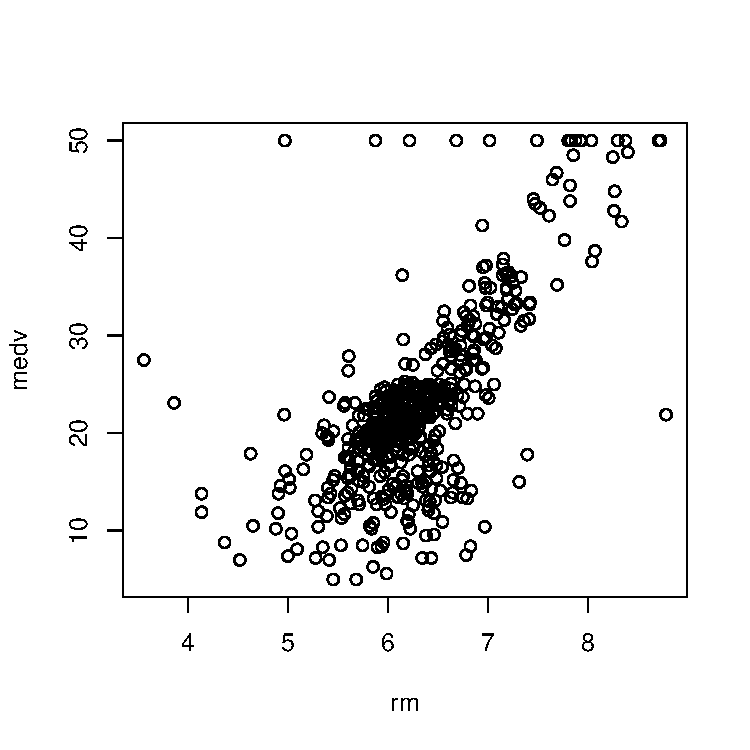
\includegraphics[width=.45\linewidth]{figure/fig-simple-house-1} 
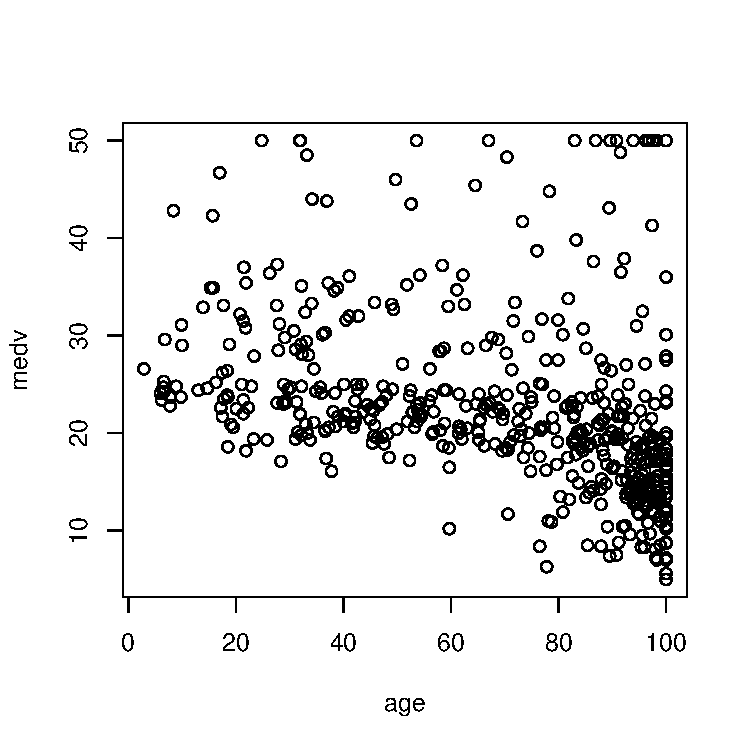
\includegraphics[width=.45\linewidth]{figure/fig-simple-house-2} 
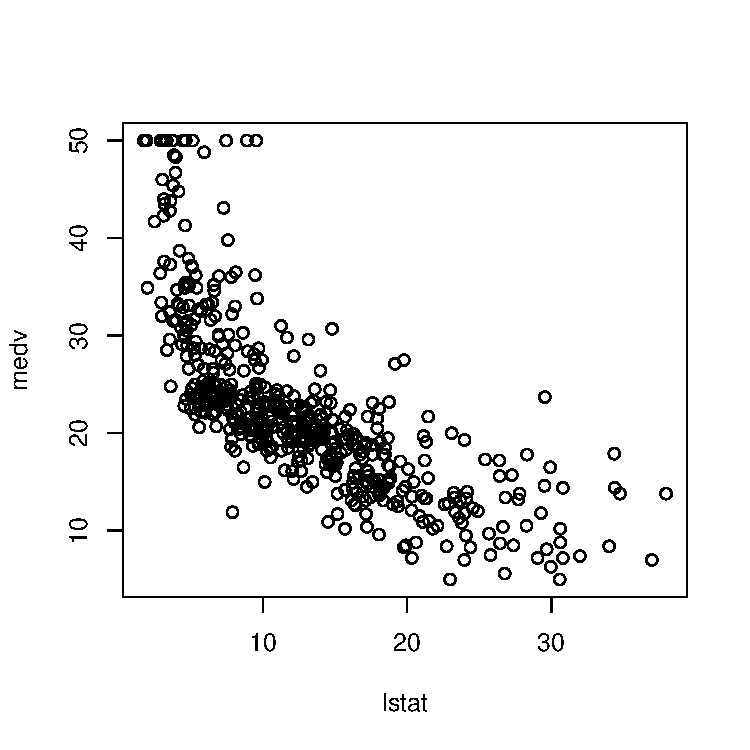
\includegraphics[width=.45\linewidth]{figure/fig-simple-house-3} 
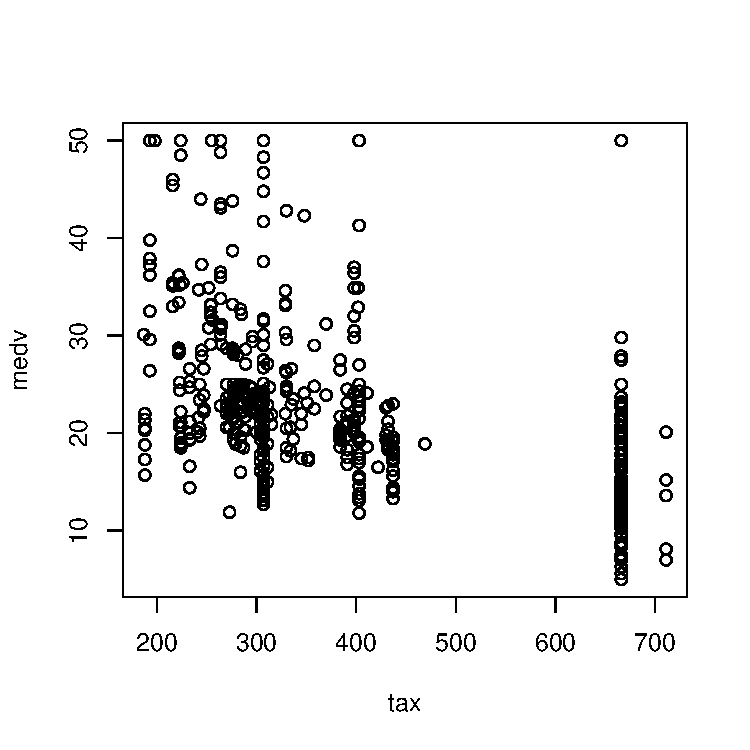
\includegraphics[width=.45\linewidth]{figure/fig-simple-house-4} 

}



\end{knitrout}
        \caption{Relation entre la variable \texttt{medv} et les
          variables \texttt{rm}, \texttt{age}, \texttt{lstat} et
          \texttt{tax} des données \texttt{house.dat}}
        \label{fig:simple:house}
      \end{figure}
    \item Les résultats ci-dessous ont été obtenus avec \textsf{R}.
\begin{knitrout}
\definecolor{shadecolor}{rgb}{0.969, 0.969, 0.969}\color{fgcolor}\begin{kframe}
\begin{alltt}
\hlstd{fit1} \hlkwb{<-} \hlkwd{lm}\hlstd{(medv} \hlopt{~} \hlstd{rm,} \hlkwc{data} \hlstd{= house)}
\hlkwd{summary}\hlstd{(fit1)}
\end{alltt}
\begin{verbatim}
## 
## Call:
## lm(formula = medv ~ rm, data = house)
## 
## Residuals:
##     Min      1Q  Median      3Q     Max 
## -23.346  -2.547   0.090   2.986  39.433 
## 
## Coefficients:
##             Estimate Std. Error t value Pr(>|t|)    
## (Intercept)  -34.671      2.650  -13.08   <2e-16 ***
## rm             9.102      0.419   21.72   <2e-16 ***
## ---
## Signif. codes:  
## 0 '***' 0.001 '**' 0.01 '*' 0.05 '.' 0.1 ' ' 1
## 
## Residual standard error: 6.616 on 504 degrees of freedom
## Multiple R-squared:  0.4835,	Adjusted R-squared:  0.4825 
## F-statistic: 471.8 on 1 and 504 DF,  p-value: < 2.2e-16
\end{verbatim}
\end{kframe}
\end{knitrout}

      On peut voir que tant l'ordonnée à l'origine que la pente sont
      très significativement différentes de zéro. La régression est
      donc elle-même significative. Cependant, le coefficient de
      détermination n'est que de $R^2 =
      0,4835$, %$
      ce qui indique que d'autres facteurs pourraient expliquer la
      variation dans \texttt{medv}.

      On calcule les bornes de l'intervalle de confiance de la
      régression avec la fonction \texttt{predict}:
\begin{knitrout}
\definecolor{shadecolor}{rgb}{0.969, 0.969, 0.969}\color{fgcolor}\begin{kframe}
\begin{alltt}
\hlstd{pred.ci} \hlkwb{<-} \hlkwd{predict}\hlstd{(fit1,} \hlkwc{interval} \hlstd{=} \hlstr{"confidence"}\hlstd{,} \hlkwc{level} \hlstd{=} \hlnum{0.95}\hlstd{)}
\end{alltt}
\end{kframe}
\end{knitrout}

      La droite de régression et ses bornes d'intervalle de confiance
      inférieure et supérieure sont illustrée à la figure
      \ref{fig:simple:house2}.
      \begin{figure}
\begin{knitrout}
\definecolor{shadecolor}{rgb}{0.969, 0.969, 0.969}\color{fgcolor}\begin{kframe}
\begin{alltt}
\hlstd{ord} \hlkwb{<-} \hlkwd{order}\hlstd{(house}\hlopt{$}\hlstd{rm)}
\hlkwd{plot}\hlstd{(medv} \hlopt{~} \hlstd{rm,} \hlkwc{data} \hlstd{= house,} \hlkwc{ylim} \hlstd{=} \hlkwd{range}\hlstd{(pred.ci))}
\hlkwd{matplot}\hlstd{(house}\hlopt{$}\hlstd{rm[ord], pred.ci[ord,],}
        \hlkwc{type} \hlstd{=} \hlstr{"l"}\hlstd{,} \hlkwc{lty} \hlstd{=} \hlkwd{c}\hlstd{(}\hlnum{1}\hlstd{,} \hlnum{2}\hlstd{,} \hlnum{2}\hlstd{),} \hlkwc{lwd}\hlstd{=} \hlnum{2}\hlstd{,}
        \hlkwc{col} \hlstd{=} \hlstr{"black"}\hlstd{,} \hlkwc{add} \hlstd{=} \hlnum{TRUE}\hlstd{)}
\end{alltt}
\end{kframe}

{\centering 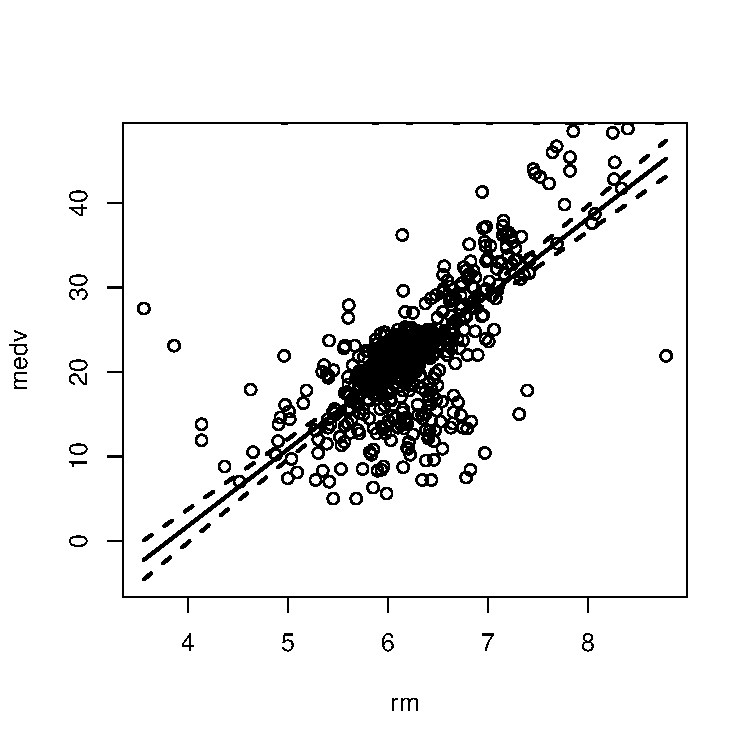
\includegraphics[width=.45\linewidth]{figure/fig-simple-house2-1} 

}



\end{knitrout}
        \caption{Résultat de la régression de la variable \texttt{rm} sur la variable \texttt{medv} des données \texttt{house.dat}}
        \label{fig:simple:house2}
      \end{figure}
    \item On reprend la même démarche, mais cette fois avec la
      variable \texttt{age}:
\begin{knitrout}
\definecolor{shadecolor}{rgb}{0.969, 0.969, 0.969}\color{fgcolor}\begin{kframe}
\begin{alltt}
\hlstd{fit2} \hlkwb{<-} \hlkwd{lm}\hlstd{(medv} \hlopt{~} \hlstd{age,} \hlkwc{data} \hlstd{= house)}
\hlkwd{summary}\hlstd{(fit2)}
\end{alltt}
\begin{verbatim}
## 
## Call:
## lm(formula = medv ~ age, data = house)
## 
## Residuals:
##     Min      1Q  Median      3Q     Max 
## -15.097  -5.138  -1.958   2.397  31.338 
## 
## Coefficients:
##             Estimate Std. Error t value Pr(>|t|)    
## (Intercept) 30.97868    0.99911  31.006   <2e-16 ***
## age         -0.12316    0.01348  -9.137   <2e-16 ***
## ---
## Signif. codes:  
## 0 '***' 0.001 '**' 0.01 '*' 0.05 '.' 0.1 ' ' 1
## 
## Residual standard error: 8.527 on 504 degrees of freedom
## Multiple R-squared:  0.1421,	Adjusted R-squared:  0.1404 
## F-statistic: 83.48 on 1 and 504 DF,  p-value: < 2.2e-16
\end{verbatim}
\begin{alltt}
\hlstd{pred.ci} \hlkwb{<-} \hlkwd{predict}\hlstd{(fit2,} \hlkwc{interval} \hlstd{=} \hlstr{"confidence"}\hlstd{,} \hlkwc{level} \hlstd{=} \hlnum{0.95}\hlstd{)}
\end{alltt}
\end{kframe}
\end{knitrout}
      La régression est encore une fois très significative. Cependant,
      le $R^2$ est encore plus faible qu'avec la variable
      \texttt{rm}. Les variables \texttt{rm} et \texttt{age}
      contribuent donc chacune à expliquer les variations de la
      variable \texttt{medv} (et \texttt{rm} mieux que \texttt{age}),
      mais aucune ne sait le faire seule de manière satisfaisante. La
      droite de régression et l'intervalle de confiance de celle-ci
      sont reproduits à la figure \ref{fig:simple:house3}. On constate
      que l'intervalle de confiance est plus large qu'en b).
      \begin{figure}
\begin{knitrout}
\definecolor{shadecolor}{rgb}{0.969, 0.969, 0.969}\color{fgcolor}\begin{kframe}
\begin{alltt}
\hlstd{ord} \hlkwb{<-} \hlkwd{order}\hlstd{(house}\hlopt{$}\hlstd{age)}
\hlkwd{plot}\hlstd{(medv} \hlopt{~} \hlstd{age,} \hlkwc{data} \hlstd{= house,} \hlkwc{ylim} \hlstd{=} \hlkwd{range}\hlstd{(pred.ci))}
\hlkwd{matplot}\hlstd{(house}\hlopt{$}\hlstd{age[ord], pred.ci[ord,],}
        \hlkwc{type} \hlstd{=} \hlstr{"l"}\hlstd{,} \hlkwc{lty} \hlstd{=} \hlkwd{c}\hlstd{(}\hlnum{1}\hlstd{,} \hlnum{2}\hlstd{,} \hlnum{2}\hlstd{),} \hlkwc{lwd} \hlstd{=} \hlnum{2}\hlstd{,}
        \hlkwc{col} \hlstd{=} \hlstr{"black"}\hlstd{,} \hlkwc{add} \hlstd{=} \hlnum{TRUE}\hlstd{)}
\end{alltt}
\end{kframe}

{\centering 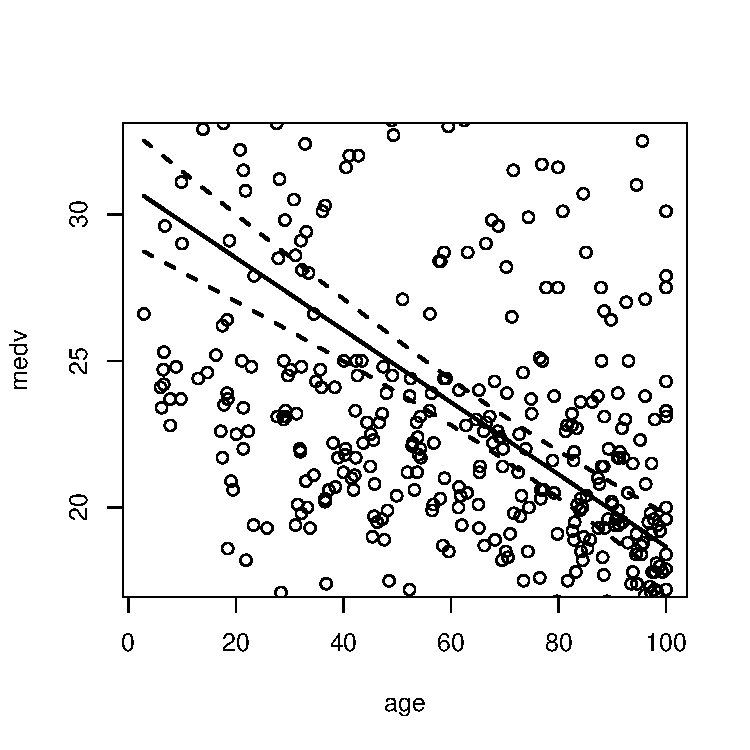
\includegraphics[width=.45\linewidth]{figure/fig-simple-house3-1} 

}



\end{knitrout}
        \caption{Résultat de la régression de la variable \texttt{age} sur la variable \texttt{medv} des données \texttt{house.dat}}
        \label{fig:simple:house3}
      \end{figure}
    \end{enumerate}
  \end{sol}
\end{exercice}

\begin{exercice}
  \label{ex:simple:carburant}
  On veut prévoir la consommation de carburant d'une automobile à
  partir de ses différentes caractéristiques physiques, notamment le
  type du moteur. Le fichier \texttt{carburant.dat} contient des
  données tirées de \emph{Consumer Reports} pour 38 automobiles des
  années modèle 1978 et 1979. Les caractéristiques fournies sont
  \begin{itemize}
  \item \texttt{mpg}: consommation de carburant en milles au gallon;
  \item \texttt{nbcyl}: nombre de cylindres (remarquer la forte
    représentation des 8 cylindres!);
  \item \texttt{cylindree}: cylindrée du moteur, en pouces cubes;
  \item \texttt{cv}: puissance en chevaux vapeurs;
  \item \texttt{poids}: poids de la voiture en milliers de livres.
  \end{itemize}
  Utiliser \textsf{R} pour faire l'analyse ci-dessous.
  \begin{enumerate}
  \item Convertir les données du fichier en unités métriques, le cas
    échéant. Par exemple, la consommation de carburant s'exprime en
    $\ell$/100~km.  Or, un gallon américain correspond à 3,785 litres
    et 1~mille à 1,6093 kilomètre. La consommation en litres aux
    100~km s'obtient donc en divisant 235,1954 par la consommation en
    milles au gallon.  De plus, 1~livre correspond à 0,45455
    kilogramme.
  \item Établir une relation entre la consommation de carburant d'une
    voiture et son poids. Vérifier la qualité de l'ajustement du
    modèle et si le modèle est significatif.
  \item Trouver un intervalle de confiance à 95~\% pour la
    consommation en carburant d'une voiture de \nombre{1350}~kg.
  \end{enumerate}

  \begin{rep}
    \begin{inparaenum}
      \stepcounter{enumi}
    \item $R^2 = 0,858$ et
      $F = 217,5$
    \item $10,57 \pm
      2,13$
    \end{inparaenum}
  \end{rep}
  \begin{sol}
    \begin{enumerate}
    \item On importe les données dans \textsf{R}, puis on effectue les
      conversions demandées. La variable \texttt{consommation}
      contient la consommation des voitures en $\ell$/100~km et la
      variable \texttt{poids} le poids en kilogrammes.
\begin{knitrout}
\definecolor{shadecolor}{rgb}{0.969, 0.969, 0.969}\color{fgcolor}\begin{kframe}
\begin{alltt}
\hlstd{carburant} \hlkwb{<-} \hlkwd{read.table}\hlstd{(}\hlstr{"carburant.dat"}\hlstd{,} \hlkwc{header} \hlstd{=} \hlnum{TRUE}\hlstd{)}
\hlstd{consommation} \hlkwb{<-} \hlnum{235.1954}\hlopt{/}\hlstd{carburant}\hlopt{$}\hlstd{mpg}
\hlstd{poids} \hlkwb{<-} \hlstd{carburant}\hlopt{$}\hlstd{poids} \hlopt{*} \hlnum{0.45455} \hlopt{*} \hlnum{1000}
\end{alltt}
\end{kframe}
\end{knitrout}
    \item La fonction \texttt{summary} fournit l'information
      essentielle pour juger de la validité et de la qualité du
      modèle:
\begin{knitrout}
\definecolor{shadecolor}{rgb}{0.969, 0.969, 0.969}\color{fgcolor}\begin{kframe}
\begin{alltt}
\hlstd{fit} \hlkwb{<-} \hlkwd{lm}\hlstd{(consommation} \hlopt{~} \hlstd{poids)}
\hlkwd{summary}\hlstd{(fit)}
\end{alltt}
\begin{verbatim}
## 
## Call:
## lm(formula = consommation ~ poids)
## 
## Residuals:
##      Min       1Q   Median       3Q      Max 
## -2.07123 -0.68380  0.01488  0.44802  2.66234 
## 
## Coefficients:
##               Estimate Std. Error t value Pr(>|t|)    
## (Intercept) -0.0146530  0.7118445  -0.021    0.984    
## poids        0.0078382  0.0005315  14.748   <2e-16 ***
## ---
## Signif. codes:  
## 0 '***' 0.001 '**' 0.01 '*' 0.05 '.' 0.1 ' ' 1
## 
## Residual standard error: 1.039 on 36 degrees of freedom
## Multiple R-squared:  0.858,	Adjusted R-squared:  0.854 
## F-statistic: 217.5 on 1 and 36 DF,  p-value: < 2.2e-16
\end{verbatim}
\end{kframe}
\end{knitrout}
      Le modèle est donc le suivant: $Y_i =
      -0,01465 +
      0,007838 x_i +
      \varepsilon_i$, $\varepsilon_i \sim N(0,
      1,039^2)$, où $Y_i$ est la
      consommation en litres aux 100 kilomètres et $x_i$ le poids en
      kilogrammes. La faible valeur $p$ du test $F$ indique une
      régression très significative. De plus, le $R^2$ de
      0,858 %$
      confirme que l'ajustement du modèle est assez bon.
    \item On veut calculer un intervalle de confiance pour la
      consommation en carburant prévue d'une voiture de
      \nombre{1350}~kg. On obtient, avec la fonction \texttt{predict}:
\begin{knitrout}
\definecolor{shadecolor}{rgb}{0.969, 0.969, 0.969}\color{fgcolor}\begin{kframe}
\begin{alltt}
\hlkwd{predict}\hlstd{(fit,} \hlkwc{newdata} \hlstd{=} \hlkwd{data.frame}\hlstd{(}\hlkwc{poids} \hlstd{=} \hlnum{1350}\hlstd{),} \hlkwc{interval} \hlstd{=} \hlstr{"prediction"}\hlstd{)}
\end{alltt}
\begin{verbatim}
##       fit      lwr     upr
## 1 10.5669 8.432089 12.7017
\end{verbatim}
\end{kframe}
\end{knitrout}
    \end{enumerate}
  \end{sol}
\end{exercice}

\begin{exercice}
On s'intéresse à l'impact du sexe sur l'espérance de vie. On connaît les durées de vie de $n_{F}=300$ femmes et $n_H=200$ hommes. On choisit d'utiliser la variable indicatrice 
$$x_{i}=\left\{ \begin{array}{ll}
0 & \mbox{, si \texttt{SEXE}}_i=\texttt{H}\\
1 & \mbox{, si \texttt{SEXE}}_i=\texttt{F}\\
\end{array}\right. .$$
On note $\bar{Y}_F$ la moyenne des durées de vie des femmes et $\bar{Y}_H$ la moyenne des durées de vie des hommes.

\begin{enumerate}
\item Montrer que l'estimateur des moindres carrés $\hat{\beta}_1$ (lié à la variable explicative $x$) est égal à $\bar{Y}_F-\bar{Y}_H$. \emph{Indice: On peut exprimer $\bar{Y}$ en termes de $\bar{Y}_F$ et $\bar{Y}_H$.} 

\item Ce résultat permet-il d'interpréter le coefficient relié à une variable catégorique binaire? Expliquer. 

\item Que représente $\hat{\beta}_0$ dans ce cas? 

\end{enumerate}
\begin{sol}
\begin{enumerate}
\item On a $$\bar{Y}=\frac{\sum_{i=1}^{500}Y_i}{500}=\frac{300\bar{Y}_F+200\bar{Y}_H}{500}.$$ Aussi,
$$\hat{\beta}_1=\frac{S_{xy}}{S_{xx}}=\frac{\sum_{i=1}^{500}x_iY_i-500\bar{x}\bar{Y}}{\sum_{i=1}^{500}x_i^2-500\bar{x}^2}.$$  Or, 
\begin{align*}
\bar{x}&=\frac{\sum_{i=1}^{500}x_i}{500}=\frac{300}{500},\\
\sum_{i=1}^{500}x_i^2&=300,\\
\sum_{i=1}^{500}x_i Y_i&=300\bar{Y}_F
\end{align*}
Donc, 
\begin{align*}
\hat{\beta}_1&=\frac{300\bar{Y}_F-500\times\frac{300}{500}\times\frac{300\bar{Y}_F+200\bar{Y}_H}{500}}{300-500\left(\frac{300}{500}\right)^2}\\
&=\frac{500\bar{Y}_F-300\bar{Y}_F-200\bar{Y}_H}{500-300}\\
&=\bar{Y}_F-\bar{Y}_H.
\end{align*}

\item Oui, le coefficient relié à la variable indicatrice qui vaut 1 si le sexe est F représente la différence etre la moyenne de l'espérance de vie pour les femmes et la moyenne de l'espérace de vie pour les hommes.

\item
\begin{align*}
\hat{\beta}_0&=\bar{Y}-\hat{\beta}_1\bar{x}=\bar{Y}-(\bar{Y}_F-\bar{Y}_H)\frac{300}{500}=\bar{Y}_H.
\end{align*}
$\Rightarrow \hat{\beta}_0$ est la moyenne de l'espérance de vie pour les hommes.

\end{enumerate}
\end{sol}
\end{exercice}

\begin{exercice}
On s'intéresse à la covariance entre deux résidus.

\begin{enumerate}
\item D'abord, trouver $\cov(Y_i,\hat{Y}_j)$. 

\item Puis, calculer $\cov(\hat{Y}_i,\hat{Y}_j)$. 

\item Déduire de a) et b) que $$\cov(\hat{\varepsilon}_i,\hat{\varepsilon}_j)=-\sigma^2\left(\frac{1}{n}+\frac{(x_i-\bar{x})(x_j-\bar{x})}{S_{xx}}\right).$$ 
\end{enumerate}

\begin{sol}
\begin{enumerate}
\item
\begin{align*}
\cov(Y_i,\hat{Y}_j)&=\cov(Y_i,\hat{\beta}_0+\hat{\beta}_1x_j)\\
&=\cov(Y_i,\bar{Y}-\hat{\beta}_1\bar{x}+\hat{\beta}_1x_j)\\
&=\cov(Y_i,\bar{Y})+(x_j-\bar{x})\cov(Y_i,\hat{\beta}_1) \mbox{ par indépendance des observations}\\
&=\frac{\sigma^2}{n}+\frac{(x_j-\bar{x})}{S_{xx}}\sum_{l=1}^n(x_l-\bar{x})\cov(Y_i,Y_l)\\
&=\frac{\sigma^2}{n}+\frac{(x_j-\bar{x})(x_i-\bar{x})}{S_{xx}}\sigma^2\mbox{ par indépendance des observations}.\\
\end{align*}

\item
\begin{align*}
\cov(\hat{Y}_i,\hat{Y}_j)&=\cov(\hat{\beta}_0+\hat{\beta}_1x_i,\hat{\beta}_0+\hat{\beta}_1x_j)\\
&=\var(\hat{\beta}_0)+(x_i+x_j)\cov(\hat{\beta}_0,\hat{\beta}_1)+x_ix_j\var(\hat{\beta}_1)\\
&=\sigma^2\left(\frac{1}{n}+\frac{\bar{x}^2}{S_{xx}}\right)-(x_i+x_j)\frac{\bar{x}\sigma^2}{S_{xx}}+x_ix_j\frac{\sigma^2}{S_{xx}}\\
&=...\\
&=\sigma^2\left(\frac{1}{n}+\frac{(x_j-\bar{x})(x_i-\bar{x})}{S_{xx}}\right).
\end{align*}

\item
\begin{align*}
\cov(\hat{\varepsilon}_i,\hat{\varepsilon}_j)&=\cov(Y_i-\hat{Y}_i,Y_j-\hat{Y}_j)\\
&=\cov(Y_i,Y_j)-\cov(Y_i,\hat{Y}_j)-\cov(\hat{Y}_i,Y_j)+\cov(\hat{Y}_i,\hat{Y}_j)\\
&=0-2\sigma^2\left(\frac{1}{n}+\frac{(x_j-\bar{x})(x_i-\bar{x})}{S_{xx}}\right)+\left(\frac{1}{n}+\frac{(x_j-\bar{x})(x_i-\bar{x})}{S_{xx}}\right)\\
&=-\sigma^2\left(\frac{1}{n}+\frac{(x_i-\bar{x})(x_j-\bar{x})}{S_{xx}}\right).
\end{align*}
\end{enumerate}
\end{sol}
\end{exercice}

\begin{exercice}
Dans un graphiques des résidus en fonction des valeurs prédites, on observe de l'hétéroscédasticité. Après une analyse plus poussée, on note que la variance de $\hat{\varepsilon}_i$ est approximativement proportionnelle à $E[Y_i]^4$ . Proposer une transformation $g$ de la variable réponse qui permettra de stabiliser la variance.
\begin{sol}
Utiliser l'approximation de Taylor de premier ordre pour montrer que la variance de $g(Y)=1/Y$ est approximativement constante.
\end{sol}
\end{exercice}

\begin{exercice}
\label{ex:simple:bact}
Les données suivantes présentent le nombre moyen de bactéries vivantes dans une boîte de conserve de nourriture et le temps (en minutes) d'exposition à une chaleur de $300^{o}$F. \footnote{Source: D. Montgomery, E.A. Peck et G.G. Vining (2012). Introduction to Linear Regression Analysis. Fifth Edition. Wiley.}

\begin{center}
\begin{tabular}{cc}
\hline
Nombre de bactéries & Temps d'exposition (min) \\ \hline
175&1\\
108&2\\
95&3\\
82&4\\
71&5\\
50&6\\
49&7\\
31&8\\
28&9\\
17&10\\
16&11\\
11&12\\ \hline
\end{tabular}
\end{center}

\begin{enumerate}
\item Tracer un nuage de points des données. Est-ce qu'un modèle de régression linéaire semble adéquat?

\item Ajuster aux données un modèle de régression linéaire. Calculer les statistiques sommaires et produire les graphiques de résidus. Interpréter les résultats. Quelles sont vos conclusions par rapport à la validité du modèle de régression?

\item Identifier une transformation pour ces données afin d'utiliser adéquatement les méthodes de régression. Ajuster ce nouveau modèle et tester la validité de la régression.
\end{enumerate}



\begin{sol}
\begin{enumerate}
\item Figure~\ref{fig:simple:bact1} shows a scatter plot of the number of bacteria versus the minutes of exposure. The plot shows a straight line would be a reasonable model, but an even better model would capture the curvature. In fact, the plot shows that when the canned food is exposed to $300^{o}$ F for a long time, there is ultimately no bacteria left. This suggests a model that would capture the asymptotic behavior of the number of bacteria when the number of minutes of exposure increases. A linear model would continue to drive down the number of bacteria, eventually leading to negative values, which is nonsensical in this context.
  
\begin{figure}
\begin{knitrout}
\definecolor{shadecolor}{rgb}{0.969, 0.969, 0.969}\color{fgcolor}

{\centering 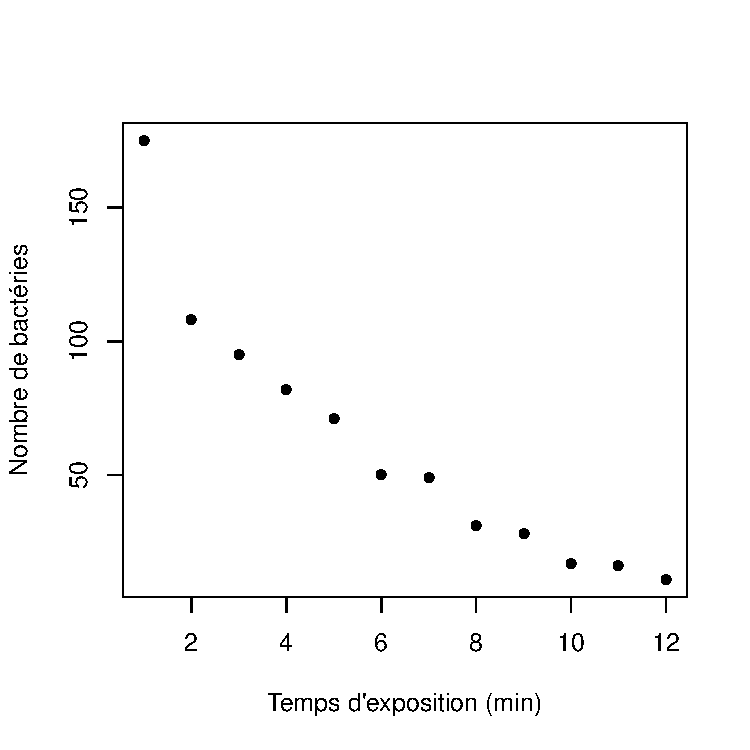
\includegraphics[width=.45\linewidth]{figure/fig-simple-bact1-1} 

}



\end{knitrout}
\caption{Scatter Plot of the Number of Bacteria versus the Minutes of Exposure to $300^{o}$ F}
\label{fig:simple:bact1}
\end{figure}
      
\item A simple linear model is fitted to the data using \textsf{R}. Here is a summary of the model:
\begin{knitrout}
\definecolor{shadecolor}{rgb}{0.969, 0.969, 0.969}\color{fgcolor}\begin{kframe}
\begin{alltt}
\hlstd{fit1} \hlkwb{<-} \hlkwd{lm}\hlstd{(bact}\hlopt{~}\hlstd{min)}
\hlkwd{summary}\hlstd{(fit1)}
\end{alltt}
\begin{verbatim}
## 
## Call:
## lm(formula = bact ~ min)
## 
## Residuals:
##     Min      1Q  Median      3Q     Max 
## -17.323  -9.890  -7.323   2.463  45.282 
## 
## Coefficients:
##             Estimate Std. Error t value Pr(>|t|)    
## (Intercept)   142.20      11.26  12.627 1.81e-07 ***
## min           -12.48       1.53  -8.155 9.94e-06 ***
## ---
## Signif. codes:  
## 0 '***' 0.001 '**' 0.01 '*' 0.05 '.' 0.1 ' ' 1
## 
## Residual standard error: 18.3 on 10 degrees of freedom
## Multiple R-squared:  0.8693,	Adjusted R-squared:  0.8562 
## F-statistic: 66.51 on 1 and 10 DF,  p-value: 9.944e-06
\end{verbatim}
\end{kframe}
\end{knitrout}
The fitted model is $$\hat{y}=142.20-12.48x,$$ where the parameters of the model are estimated by the best linear unbiased estimators. The ANOVA table is obtained using \textsf{R}:
\begin{knitrout}
\definecolor{shadecolor}{rgb}{0.969, 0.969, 0.969}\color{fgcolor}\begin{kframe}
\begin{alltt}
\hlkwd{anova}\hlstd{(fit1)}
\end{alltt}
\begin{verbatim}
## Analysis of Variance Table
## 
## Response: bact
##           Df  Sum Sq Mean Sq F value    Pr(>F)    
## min        1 22268.8 22268.8  66.512 9.944e-06 ***
## Residuals 10  3348.1   334.8                      
## ---
## Signif. codes:  
## 0 '***' 0.001 '**' 0.01 '*' 0.05 '.' 0.1 ' ' 1
\end{verbatim}
\end{kframe}
\end{knitrout}

In order to test for the significance of regression, we use the F-statistic. The F-statistic is 66.512, and it has 1 and 10 degrees of freedom, so the $p$-value is $$P[F_{(1,10)}>66.512]=9.944\times10^{-6} .$$ Since the $p$-value is much smaller than 1\%, there is enough evidence to reject the null hypothesis that $\beta_{1}=0$ at the 1\% level. The simple linear model is significant.

The value of $R^{2}$ is $86.93\%$. This is a high coefficient of correlation, it means that about 87\% of the variation in the number of bacteria in the canned food is explained by the minutes of exposure to $300^{o}$F. The model seems to perform well.

The Q-Q Plot of the studentized residuals is shown in Figure~\ref{fig:simple:bact2}. The line represents when the empirical quantiles are exactly equal to the standard normal quantiles. The normality assumption is seriously violated as the dots are clearly not on a straight line. This means there are serious flaws in the model, including the fact that the hypothesis tests are not reliable.

\begin{figure}
\begin{knitrout}
\definecolor{shadecolor}{rgb}{0.969, 0.969, 0.969}\color{fgcolor}

{\centering 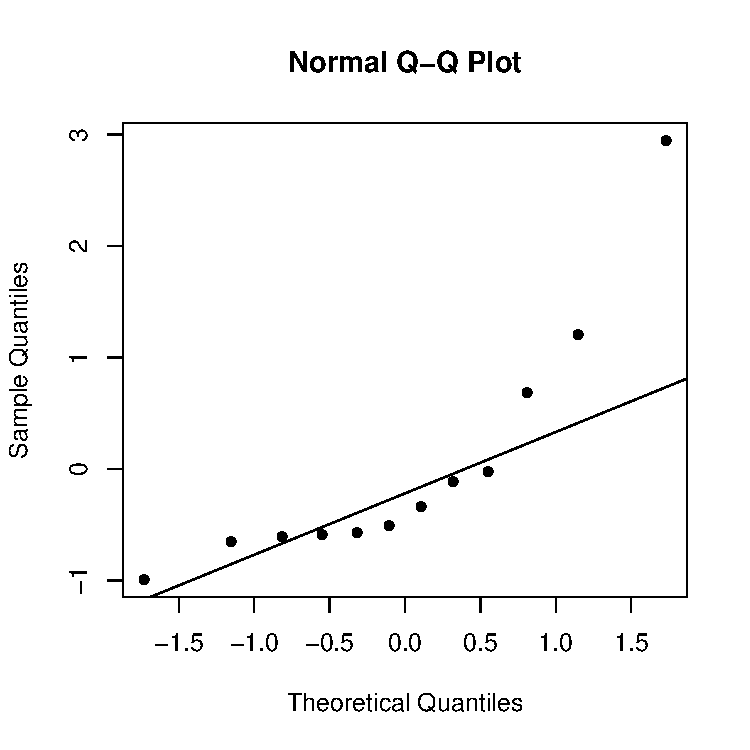
\includegraphics[width=.45\linewidth]{figure/fig-simple-bact2-1} 

}



\end{knitrout}
\caption{Q-Q Plot for Simple Linear Model in Problem \ref{chap:simple}.\ref{ex:simple:bact}} 
\label{fig:simple:bact2}
\end{figure}

\begin{figure}
\begin{knitrout}
\definecolor{shadecolor}{rgb}{0.969, 0.969, 0.969}\color{fgcolor}

{\centering 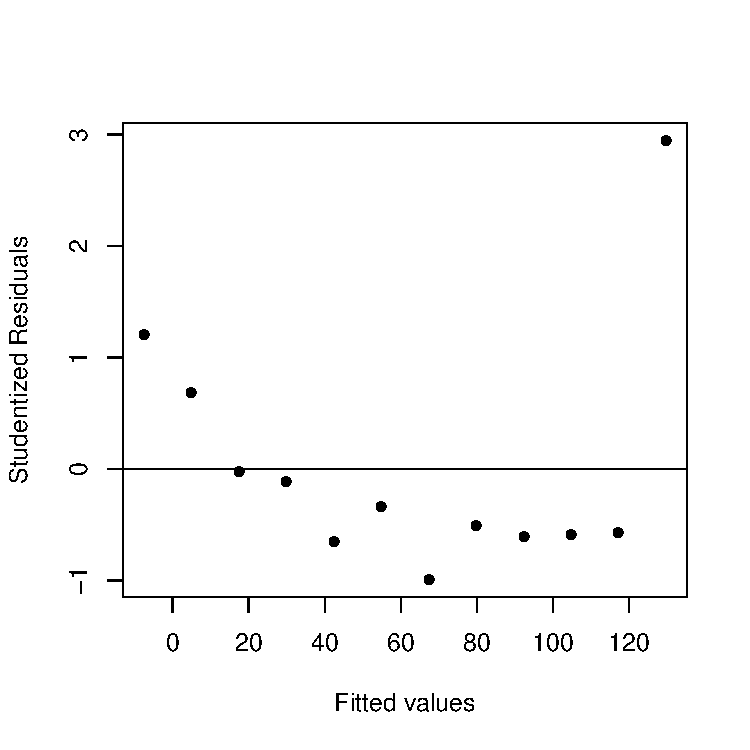
\includegraphics[width=.45\linewidth]{figure/fig-simple-bact3-1} 

}



\end{knitrout}
\caption{Residuals versus the Fitted Values for Simple Linear Model in Problem \ref{chap:simple}.\ref{ex:simple:bact}} \label{fig:simple:bact3}
\end{figure}

Figure~\ref{fig:simple:bact3} shows a plot of the studentized residuals versus the fitted values. The plot suggests a clear curve, which is usually an indicator of non-linearity. This is in line with the previous comments.

Finally, this model is inadequate and transformations on the response variables are required.

\item The Box-Cox method is used to determine which transformation is optimal. Figure~\ref{fig:simple:bact4} shows the plot of the log-likelihood function in terms of $\lambda$, for two different ranges of $\lambda$. It was obtained with the \textsf{R} commands:
\begin{knitrout}
\definecolor{shadecolor}{rgb}{0.969, 0.969, 0.969}\color{fgcolor}\begin{kframe}
\begin{alltt}
\hlkwd{boxcox}\hlstd{(bact}\hlopt{~}\hlstd{min,} \hlkwc{lambda} \hlstd{=} \hlkwd{seq}\hlstd{(}\hlopt{-}\hlnum{2}\hlstd{,} \hlnum{2}\hlstd{,} \hlkwc{len} \hlstd{=} \hlnum{20}\hlstd{),} \hlkwc{plotit} \hlstd{=} \hlnum{TRUE}\hlstd{)}
\hlkwd{boxcox}\hlstd{(bact}\hlopt{~}\hlstd{min,} \hlkwc{lambda} \hlstd{=} \hlkwd{seq}\hlstd{(}\hlopt{-}\hlnum{0.2}\hlstd{,} \hlnum{0.5}\hlstd{,} \hlkwc{len} \hlstd{=} \hlnum{20}\hlstd{),} \hlkwc{plotit} \hlstd{=} \hlnum{TRUE}\hlstd{)}
\end{alltt}
\end{kframe}
\end{knitrout}

\begin{figure}
\begin{knitrout}
\definecolor{shadecolor}{rgb}{0.969, 0.969, 0.969}\color{fgcolor}

{\centering 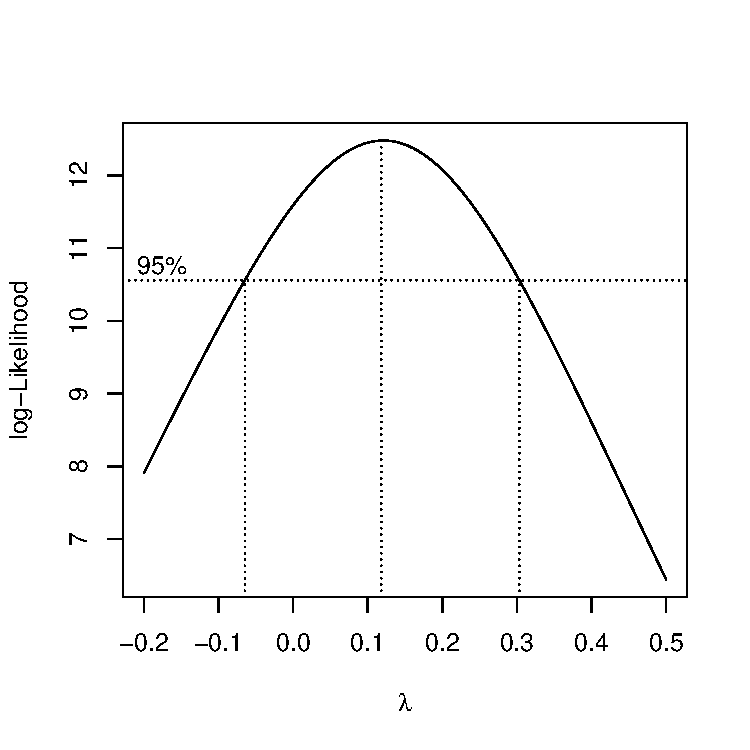
\includegraphics[width=.45\linewidth]{figure/fig-simple-bact4-1} 
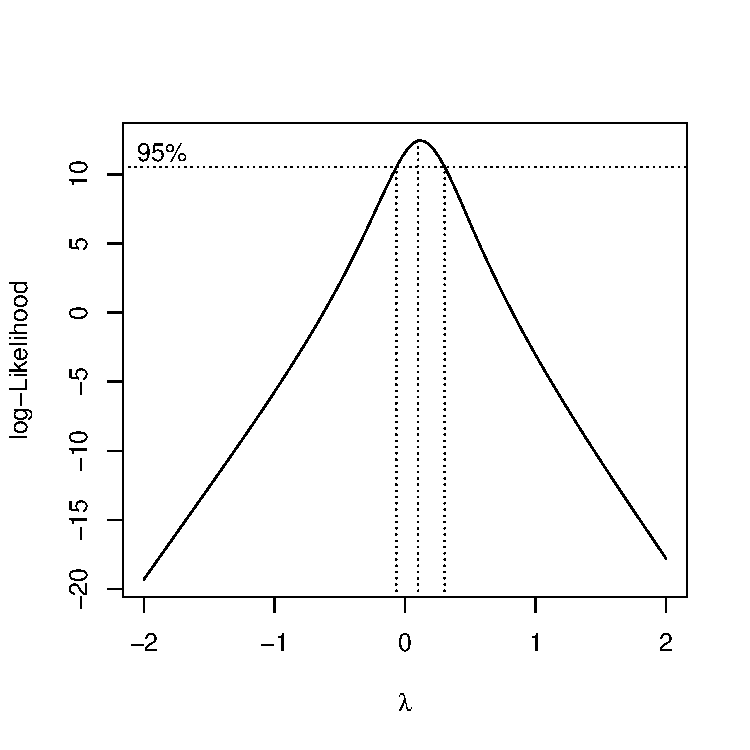
\includegraphics[width=.45\linewidth]{figure/fig-simple-bact4-2} 

}



\end{knitrout}
\caption{Log-likelihood versus $\lambda$ in the Box-Cox method for Problem \ref{chap:simple}.\ref{ex:simple:bact}} \label{fig:simple:bact4}
\end{figure}

Note that the maximum is around 0.1 and 0 is included in the 95\% confidence interval for $\lambda$. Therefore, it is preferable to use 0 as this is a common transformation, it represents the logarithm transformation. Let $y^{*}=\ln(y)$. A simple linear model is fitted to the transformed data. The output is the following:
\begin{knitrout}
\definecolor{shadecolor}{rgb}{0.969, 0.969, 0.969}\color{fgcolor}\begin{kframe}
\begin{alltt}
\hlstd{logbact} \hlkwb{<-} \hlkwd{log}\hlstd{(bact)}
\hlstd{fit2} \hlkwb{<-} \hlkwd{lm}\hlstd{(logbact}\hlopt{~}\hlstd{min)}
\hlkwd{summary}\hlstd{(fit2)}
\end{alltt}
\begin{verbatim}
## 
## Call:
## lm(formula = logbact ~ min)
## 
## Residuals:
##       Min        1Q    Median        3Q       Max 
## -0.184303 -0.083994  0.001453  0.072825  0.206246 
## 
## Coefficients:
##             Estimate Std. Error t value Pr(>|t|)    
## (Intercept)  5.33878    0.07409   72.05 6.47e-15 ***
## min         -0.23617    0.01007  -23.46 4.49e-10 ***
## ---
## Signif. codes:  
## 0 '***' 0.001 '**' 0.01 '*' 0.05 '.' 0.1 ' ' 1
## 
## Residual standard error: 0.1204 on 10 degrees of freedom
## Multiple R-squared:  0.9822,	Adjusted R-squared:  0.9804 
## F-statistic: 550.3 on 1 and 10 DF,  p-value: 4.489e-10
\end{verbatim}
\end{kframe}
\end{knitrout}

The fitted model is $$\hat{y}^{*}=5.33878-0.23617x,$$ where the parameters of the model are estimated by the best linear unbiased estimators. Figure~\ref{fig:simple:bact5} is a scatter plot of the transformed response variable versus the covariate, along with the fitted line. The scatter plot looks much more linear now than in (a).

\begin{figure}
\begin{knitrout}
\definecolor{shadecolor}{rgb}{0.969, 0.969, 0.969}\color{fgcolor}

{\centering 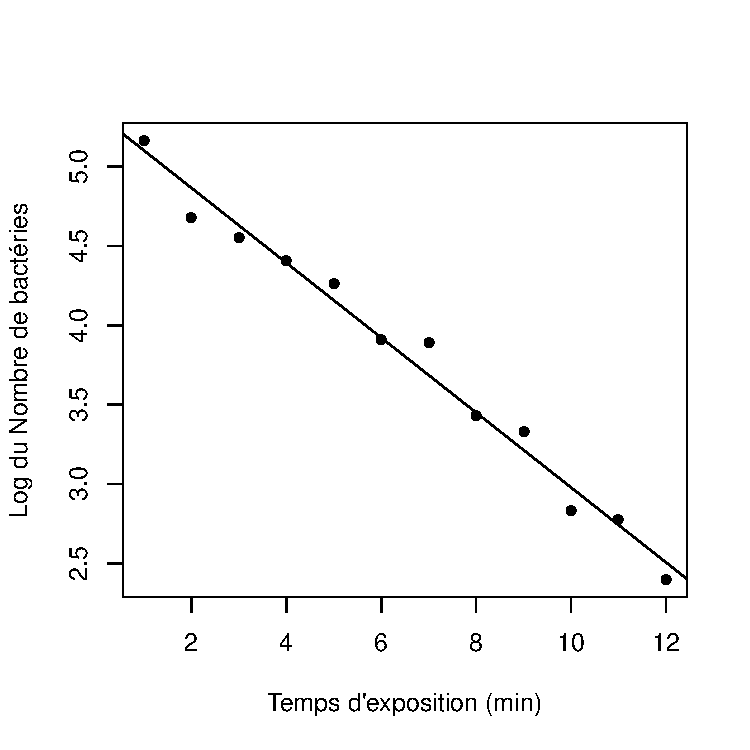
\includegraphics[width=.45\linewidth]{figure/fig-simple-bact5-1} 

}



\end{knitrout}
\caption{Scatter Plot of the Logarithm of the Number of Bacteria versus the Minutes of Exposure to $300^{o}$ F}
\label{fig:simple:bact5}
\end{figure}

The ANOVA table is obtained using \textsf{R}:
\begin{knitrout}
\definecolor{shadecolor}{rgb}{0.969, 0.969, 0.969}\color{fgcolor}\begin{kframe}
\begin{alltt}
\hlkwd{anova}\hlstd{(fit2)}
\end{alltt}
\begin{verbatim}
## Analysis of Variance Table
## 
## Response: logbact
##           Df Sum Sq Mean Sq F value    Pr(>F)    
## min        1 7.9761  7.9761  550.33 4.489e-10 ***
## Residuals 10 0.1449  0.0145                      
## ---
## Signif. codes:  
## 0 '***' 0.001 '**' 0.01 '*' 0.05 '.' 0.1 ' ' 1
\end{verbatim}
\end{kframe}
\end{knitrout}

The F-statistic for the test of significance of regression is 550.33, and it has 1 and 10 degrees of freedom, so the $p$-value is $$P[F_{(1,10)}>550.33]= 4.489\times10^{-10}.$$ Since the $p$-value is much smaller than 1\%, there is enough evidence to reject the null hypothesis that $\beta_{1}=0$ at the 1\% level. This model is significant.

The value of $R^{2}$ is very high at $98.22\%$. This means that about 98\% of the variation in the log of the number of bacteria in the canned food is explained by the minutes of exposure to $300^{o}$F. The model seems to perform very well, better than the model proposed in (b).

The Q-Q Plot of the studentized residuals is shown in Figure~\ref{fig:simple:bact6}. The dots are beautifully aligned with the standard normal quantiles. The normality assumption is appropriate. Figure~\ref{fig:simple:bact7} shows a plot of the studentized residuals versus the fitted values. The dots can be contained in horizontal bands and looks randomly scattered.

Finally, this model is adequate and the transformation used on the response variables fixed the problems in the model.

\begin{figure}
\begin{knitrout}
\definecolor{shadecolor}{rgb}{0.969, 0.969, 0.969}\color{fgcolor}

{\centering 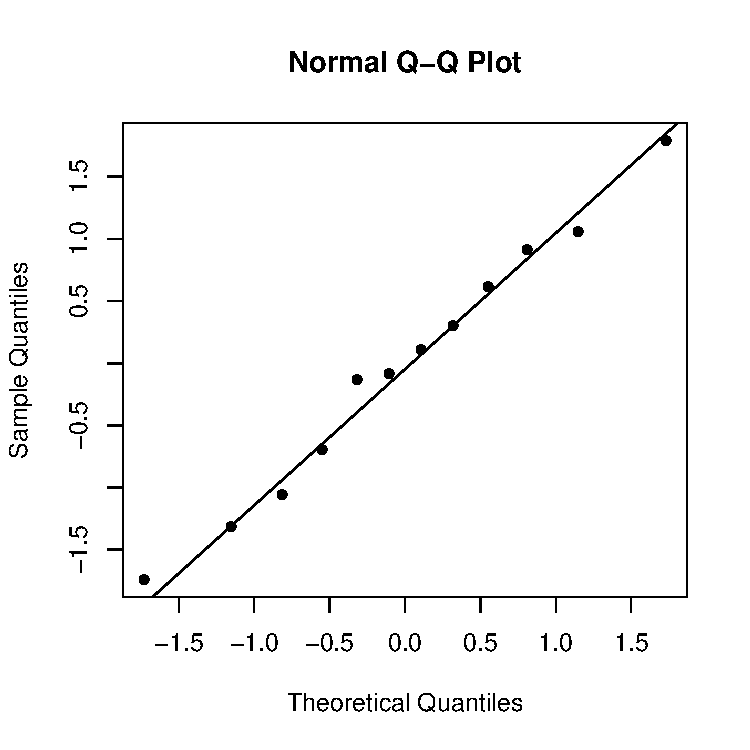
\includegraphics[width=.45\linewidth]{figure/fig-simple-bact6-1} 

}



\end{knitrout}
\caption{Q-Q Plot of Model for the Logarithm of the Number of Bacteria in Problem \ref{chap:simple}.\ref{ex:simple:bact}} \label{fig:simple:bact6}
\end{figure}

\begin{figure}
\begin{knitrout}
\definecolor{shadecolor}{rgb}{0.969, 0.969, 0.969}\color{fgcolor}

{\centering 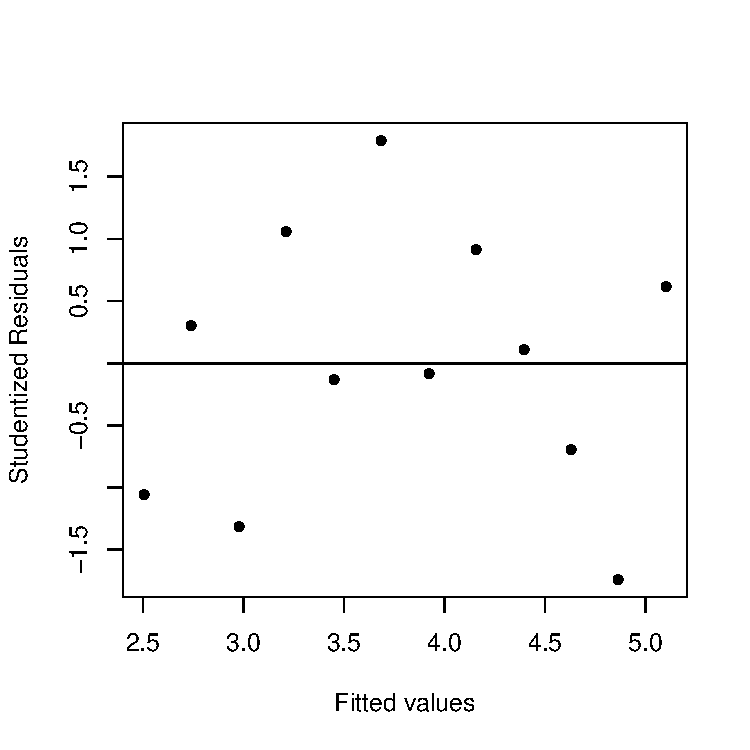
\includegraphics[width=.45\linewidth]{figure/fig-simple-bact7-1} 

}



\end{knitrout}
\caption{Residuals versus the Fitted Values for Model for the Logarithm of the Number of Bacteria in Problem \ref{chap:simple}.\ref{ex:simple:bact}} 
\label{fig:simple:bact7}
\end{figure}

\end{enumerate}
\end{sol}

\end{exercice}

\Closesolutionfile{solutions}
\Closesolutionfile{reponses}

%%%
%%% Insérer les réponses
%%%
\bigskip
\section*{Réponses}

\begin{reponse}{2.1}
    \begin{inparaenum}
      \stepcounter{enumi}
      \stepcounter{enumi}
    \item $\hat{\beta}_0=66.44882$ et $\hat{\beta}_1=-0.8407468$
    \item $\hat{Y}_1 = 11,80, \hat{Y}_2 = 30,30, \hat{Y}_3 = 29,46,
      \hat{Y}_4 = 16,84, \hat{Y}_5 = 16,00, \hat{Y}_6 = 24,41,
      \hat{Y}_7 = 22,73, \hat{Y}_8 = 34,50, \hat{Y}_9 = 31,14,
      \hat{Y}_{10} = 32,82$
    \end{inparaenum}
  
\end{reponse}
\begin{reponse}{2.2}
    \begin{inparaenum}
    \item $\hat{\beta}_0=7$ et $\hat{\beta}_1=-0,5$
    \item SST = 14, SSR = 7, SSE = 7, MSR = 7, MSE = 7/6, $F$ = 6, $R^2$ = 0,5
    \end{inparaenum}
  
\end{reponse}
\begin{reponse}{2.3}
    \begin{inparaenum}
      \stepcounter{enumi}
    \item
      $\hat{\beta}_0 = -87,5167$
      et
      $\hat{\beta}_1 = 3,45$
      \stepcounter{enumi}
    \item $R^2 = 0,991$
    \item
      $\SSR = 3332,7$
      $\SSE = 30,23$ et
      $\SST = 3362,93$
    \end{inparaenum}
  
\end{reponse}
\begin{reponse}{2.5}
    $\hat{\beta}_0 = \bar{Y} - \hat{\beta}_1 (n + 1)/2$,
    $\hat{\beta}_1 = (12 \sum_{t = 0}^n t Y_i - 6 n (n + 1)
    \bar{Y})/(n (n^2 - 1)$
  
\end{reponse}
\begin{reponse}{2.6}
    \begin{inparaenum}
    \item $\hat{\beta}= \sum_{i = 1}^n x_i Y_i/\sum_{i = 1}^n x_i^2$
      \stepcounter{enumi}
    \item $\var{\hat{\beta}} = \sigma^2/\sum_{i = 1}^n x_i^2$
    \end{inparaenum}
  
\end{reponse}
\begin{reponse}{2.9}
    \begin{enumerate}
    \item $\hat{\beta}_1^\prime = (b/d) \hat{\beta}_1$
    \end{enumerate}
  
\end{reponse}
\begin{reponse}{2.11}
    $\beta_1 \in \hat{\beta}_1 \pm z_{\alpha/2} \sigma
    \left( \sum_{i=1}^n (x_i - \bar{x})^2 \right)^{-1/2}$
  
\end{reponse}
\begin{reponse}{2.12}
    $(-1,5, -0,7)$
  
\end{reponse}
\begin{reponse}{2.13}
    \begin{inparaenum}
    \item $\hat{\beta}_0 = 9,273$, $\hat{\beta}_1 = 1,436$
    \item $t = 9,809$
    \item $(1,105, 1,768)$
    \end{inparaenum}
  
\end{reponse}
\begin{reponse}{2.14}
    $F = 0,73$, valeur $p$: $0,397$
  
\end{reponse}
\begin{reponse}{2.15}
    $\hat{Y}_0 \pm t_{\alpha/2}(n - 1)\, s\,
    \sqrt{1 + x_0^2/\sum_{i=1}^n x_i^2}$
  
\end{reponse}
\begin{reponse}{2.16}
    \begin{inparaenum}
    \item $\text{PNB} = 1,168 + 1,716 \text{ MM}$
    \item $\beta_0 \in (0,060, 2,276)$, $\beta_1 \in (1,427, 2,005)$
    \item $6,31$
    \item $(11,20, 12,80)$ et $(10,83, 13,17)$
    \end{inparaenum}
  
\end{reponse}
\begin{reponse}{2.18}
    \begin{inparaenum}
      \stepcounter{enumi}
    \item $R^2 = 0,858$ et
      $F = 217,5$
    \item $10,57 \pm
      2,13$
    \end{inparaenum}
  
\end{reponse}



%%% Local Variables:
%%% mode: latex
%%% TeX-master: "exercices_methodes_statistiques"
%%% End:


\chapter{Régression linéaire multiple}
\label{chap:multiple}

\Opensolutionfile{reponses}[reponses-multiple]
\Opensolutionfile{solutions}[solutions-multiple]

\begin{Filesave}{reponses}
\bigskip
\section*{Réponses}

\end{Filesave}

\begin{Filesave}{solutions}
\section*{Chapitre \ref{chap:multiple}}
\addcontentsline{toc}{section}{Chapitre \protect\ref{chap:multiple}}

\end{Filesave}




\begin{exercice}
  \label{ex:multiple:preuve}
  Considérer le modèle de régression linéaire $\mat{y} = \mat{X}
  \betab + \vepsb$, où $\mat{X}$ est une matrice $n \times (p+1)$.
  Démontrer, en dérivant
  \begin{align*}
    S(\betab)
    &= \sum_{t=1}^n (Y_t - \mat{x}_t^\prime \betab)^2 \\
    &= (\mat{y} - \mat{X} \betab)^\prime (\mat{y} - \mat{X} \betab)
  \end{align*}
  par rapport à $\betab$, que les équations normales à résoudre pour
  obtenir l'estimateur des moindres carrés de $\betab$ sont, sous
  forme matricielle,
  \begin{displaymath}
    (\mat{X}^\prime \mat{X}) \betabh = \mat{X}^\prime \mat{y},
  \end{displaymath}
  Déduire l'estimateur des moindres carrés de ces équations.
  \emph{Astuce}: utiliser le théorème
  \ref{thm:elements:derivee_fonction} de l'annexe \ref{chap:elements}.
  \begin{sol}
    Tout d'abord, selon le théorème
    \ref{thm:elements:derivee_fonction} de l'annexe
    \ref{chap:elements},
    \begin{displaymath}
      \frac{d}{d \mat{x}}\, f(\mat{x})^\prime \mat{A} f(\mat{x}) =
      2 \left( \frac{d}{d \mat{x}} f(\mat{x}) \right)^\prime \mat{A} f(\mat{x}).
    \end{displaymath}
    Il suffit, pour faire la démonstration, d'appliquer directement ce
    résultat à la forme quadratique
    \begin{displaymath}
      S(\betab) = (\mat{y} - \mat{X} \betab)^\prime (\mat{y} - \mat{X} \betab)
    \end{displaymath}
    avec $f(\betab) = \mat{y} - \mat{X} \betab$ et $\mat{A} =
    \mat{I}$, la matrice identité. On a alors
    \begin{align*}
      \frac{d}{d\betab} S(\betab)
      &= 2
      \left(
        \frac{d}{d\betab} (\mat{y} - \mat{X} \betab)
      \right)^\prime
      \mat{y} - \mat{X} \betab \\
      &= 2 (-\mat{X})^\prime (\mat{y} - \mat{X} \betab)\\
      &= -2 \mat{X}^\prime (\mat{y} - \mat{X} \betab).
    \end{align*}
    En posant ces dérivées exprimées sous forme matricielle
    simultanément égales à zéro, on obtient les équations normales à
    résoudre pour calculer l'estimateur des moindres carrés du vecteur
    $\betab$, soit
    \begin{displaymath}
      \mat{X}^\prime \mat{X} \betabh = \mat{X}^\prime \mat{y}.
    \end{displaymath}
    En isolant $\betabh$ dans l'équation ci-dessus, on obtient,
    finalement, l'estimateur des moindres carrés:
    \begin{displaymath}
      \betabh = (\mat{X}^\prime \mat{X})^{-1} \mat{X}^\prime \mat{y}.
    \end{displaymath}
  \end{sol}
\end{exercice}

\begin{exercice}
  Pour chacun des modèles de régression ci-dessous, spécifier la
  matrice de schéma $\mat{X}$ dans la représentation $\mat{y} =
  \mat{X} \betab + \vepsb$ du modèle, puis obtenir, si possible, les
  formules explicites des estimateurs des moindres carrés des
  paramètres.
  \begin{enumerate}
  \item $Y_t = \beta_0 + \varepsilon_t$
  \item $Y_t = \beta_1 X_t + \varepsilon_t$
  \item $Y_t = \beta_0 + \beta_1 X_{t1} + \beta_2 X_{t2} +
    \varepsilon_t$
  \end{enumerate}
  \begin{rep}
    \begin{inparaenum}
      \item $\hat{\beta}_0 = \bar{Y}$
      \item $\hat{\beta}_1 = (\sum_{t=1}^n X_t Y_t)/(\sum_{t=1}^n X_t^2)$
      \end{inparaenum}
  \end{rep}
  \begin{sol}
    \begin{enumerate}
    \item On a un modèle sans variable explicative. Intuitivement, la
      meilleure prévision de $Y_t$ sera alors $\bar{Y}$. En effet,
      pour ce modèle,
      \begin{displaymath}
        \mat{X} =
        \begin{bmatrix}
          1 \\ \vdots \\ 1
        \end{bmatrix}_{n \times 1}
      \end{displaymath}
      et
      \begin{align*}
        \betabh
        &=\left(\mat{X}^\prime \mat{X} \right)^{-1} \mat{X}^\prime
        \mat{y} \\
        &=
        \left(
          \begin{bmatrix}
            1 & \cdots & 1
          \end{bmatrix}
          \begin{bmatrix}
            1 \\ \vdots \\ 1
          \end{bmatrix}
        \right)^{-1}
        \begin{bmatrix}
          1 & \cdots & 1
        \end{bmatrix}
        \begin{bmatrix}
          Y_1 \\ \vdots \\ Y_n
        \end{bmatrix}\\
        &= n^{-1} \sum_{t=1}^n Y_t \\
        &= \bar{Y}.
      \end{align*}
    \item Il s'agit du modèle de régression linéaire simple passant
      par l'origine, pour lequel la matrice de schéma est
      \begin{displaymath}
        \mat{X} =
        \begin{bmatrix}
          X_1 \\ \vdots \\ X_n
        \end{bmatrix}_{n \times 1}.
      \end{displaymath}
      Par conséquent,
      \begin{align*}
        \betabh
        &=
        \left(
          \begin{bmatrix}
            X_1 & \cdots & X_n
          \end{bmatrix}
          \begin{bmatrix}
            X_1 \\ \vdots \\ X_n
          \end{bmatrix}
        \right)^{-1}
        \begin{bmatrix}
          X_1 & \cdots & X_n
        \end{bmatrix}
        \begin{bmatrix}
          Y_1 \\ \vdots \\ Y_n
        \end{bmatrix} \\
        &=
        \left(
          \sum_{t=1}^n X_t^2
        \right)^{-1} \sum_{t=1}^n X_tY_t \\
        &= \frac{\sum_{t=1}^n X_t Y_t}{\sum_{t=1}^n X_t^2},
      \end{align*}
      tel qu'obtenu à l'exercice
      \ref{chap:simple}.\ref{ex:simple:origine}.
    \item On est ici en présence d'un modèle de régression multiple ne
      passant pas par l'origine et ayant deux variables explicatives.
      La matrice de schéma est alors
      \begin{displaymath}
        \mat{X} =
        \begin{bmatrix}
          1      & X_{11}  & X_{12} \\
          \vdots & \vdots & \vdots \\
          1      & X_{n1}  & X_{n2}
        \end{bmatrix}_{n \times 3}.
      \end{displaymath}
      Par conséquent,
      \begin{align*}
        \betabh
        &=
        \left(
          \begin{bmatrix}
            1     & \cdots & 1      \\
            X_{11} & \cdots & X_{n1} \\
            X_{12} & \cdots & X_{n2}
          \end{bmatrix}
          \begin{bmatrix}
            1      & X_{11}  & X_{12} \\
            \vdots & \vdots & \vdots \\
            1      & X_{n1}  & X_{n2}
          \end{bmatrix}
        \right)^{-1}
        \begin{bmatrix}
          1     & \cdots & 1      \\
          X_{11} & \cdots & X_{n1} \\
          X_{12} & \cdots & X_{n2}
        \end{bmatrix}
        \begin{bmatrix}
          Y_1 \\ \vdots \\ Y_n
        \end{bmatrix} \\
        & =
        \begin{bmatrix}
          n           & n \bar{X}_1             & n \bar{X}_2 \\
          n \bar{X}_1 & \sum_{t=1}^n X_{t1}^2    & \sum_{t=1}^n X_{t1}X_{t2} \\
          n \bar{X}_2 & \sum_{t=1}^n X_{t1}X_{t2} & \sum_{t=1}^n X_{t2}^2
        \end{bmatrix}^{-1}
        \begin{bmatrix}
          \sum_{t=1}^n Y_t \\ \sum_{t=1}^n X_{t1}Y_t \\ \sum_{t=1}^n
          X_{t2}Y_t
        \end{bmatrix}.
      \end{align*}
      L'inversion de la première matrice et le produit par la seconde
      sont laissés aux bons soins du lecteur plus patient que les
      rédacteurs de ces solutions.
    \end{enumerate}
  \end{sol}
\end{exercice}

\begin{exercice}
  Vérifier, pour le modèle de régression linéaire simple, que les
  valeurs trouvées dans la matrice de variance-covariance
  $\var{\betabh} = \sigma^2 (\mat{X}^\prime \mat{X})^{-1}$
  correspondent à celles calculées au chapitre \ref{chap:simple}.
  \begin{sol}
    Dans le modèle de régression linéaire simple, la matrice schéma est
    \begin{displaymath}
      \mat{X} =
      \begin{bmatrix}
        1      & X_1    \\
        \vdots & \vdots \\
        1      & X_n
      \end{bmatrix}.
    \end{displaymath}
    Par conséquent,
    \begin{align*}
      \var{\betabh}
      &= \sigma^2 (\mat{X}^\prime \mat{X})^{-1} \\
      &= \sigma^2
      \left(
        \begin{bmatrix}
          1   & \cdots & 1  \\
          X_1 & \cdots & X_n
        \end{bmatrix}
        \begin{bmatrix}
          1      & X_1    \\
          \vdots & \vdots \\
          1      & X_n
        \end{bmatrix}
      \right)^{-1} \\
      &= \sigma^2
      \begin{bmatrix}
        n         & n \bar{X}        \\
        n \bar{X} & \sum_{t=1}^n X_t^2
      \end{bmatrix}^{-1}\\
      &= \frac{\sigma^2}{n \sum_{t=1}^n X_t^2 - n^2 \bar{X}^2}
      \begin{bmatrix}
        \sum_{t=1}^n X_t^2 & -n \bar{X} \\
        -n \bar{X}        & n
      \end{bmatrix} \\
      &= \frac{\sigma^2}{\sum_{t=1}^n (X_t - \bar{X}^2)}
      \begin{bmatrix}
        n^{-1} \sum_{t=1}^n X_t^2 & -\bar{X} \\
        -\bar{X}                 & 1
      \end{bmatrix},
    \end{align*}
    d'où
    \begin{align*}
      \var{\hat{\beta}_0}
      &= \sigma^2\, \frac{\sum_{t=1}^n X_t^2}{%
        n \sum_{t=1}^n (X_t - \bar{X})^2} \\
      &= \sigma^2\, \frac{\sum_{t=1}^n (X_t - \bar{X}^2) + n \bar{X}^2}{%
        n \sum_{t=1}^n (X_t - \bar{X})^2} \\
      \intertext{et}
      \var{\hat{\beta}_1}
      &= \frac{\sigma^2}{\sum_{t=1}^n (X_t - \bar{X})^2}.
    \end{align*}
    Ceci correspond aux résultats antérieurs.
  \end{sol}
\end{exercice}

\begin{exercice}
  Démontrer les relations ci-dessous dans le contexte de la régression
  linéaire multiple et trouver leur équivalent en régression linéaire
  simple. Utiliser $\mat{e} = \mat{y - \hat{y}}$.
  \begin{enumerate}
  \item $\mat{X}^\prime \mat{e} = \mat{0}$
  \item $\mat{\hat{y}}^\prime \mat{e} = 0$
  \item $\mat{\hat{y}}^\prime \mat{\hat{y}} = \betabh^\prime
    \mat{X}^\prime \mat{y}$
  \end{enumerate}
  \begin{sol}
    Dans les démonstrations qui suivent, trois relations de base
    seront utilisées:
    $\mat{e} = \mat{y - \hat{y}}$,
    $\mat{\hat{y}} = \mat{X} \betabh$ et
    $\betabh = (\mat{X}^\prime \mat{X})^{-1} \mat{X}^\prime \mat{y}$.
    \begin{enumerate}
    \item On a
      \begin{align*}
        \mat{X}^\prime \mat{e}
        &= \mat{X}^\prime (\mat{y - \hat{y}}) \\
        &= \mat{X}^\prime (\mat{y} - \mat{X} \betabh) \\
        &= \mat{X}^\prime \mat{y} - (\mat{X}^\prime \mat{X}) \betabh \\
        &= \mat{X}^\prime \mat{y} - (\mat{X}^\prime \mat{X})
        (\mat{X}^\prime \mat{X})^{-1} \mat{X}^\prime \mat{y} \\
        &= \mat{X}^\prime \mat{y} - \mat{X}^\prime \mat{y} \\
        &= \mat{0}.
      \end{align*}
      En régression linéaire simple, cela donne
      \begin{align*}
        \mat{X}^\prime \mat{e} &=
        \begin{bmatrix}
          1   & \cdots & 1  \\
          X_1 & \cdots & X_n
        \end{bmatrix}
        \begin{bmatrix}
          e_1 \\ \vdots \\ e_n
        \end{bmatrix} \\
        &=
        \begin{bmatrix}
          \sum_{t=1}^n e_t \\
          \sum_{t=1}^n X_t e_t
        \end{bmatrix}.
      \end{align*}
      Par conséquent, $\mat{X}^\prime \mat{e} = \mat{0}$ se simplifie
      en $\sum_{t=1}^n e_t = 0$ et $\sum_{t=1}^n X_t e_t = 0$ soit,
      respectivement, la condition pour que l'estimateur des moindres
      carrés soit sans biais et la seconde équation normale obtenue à
      la partie \ref{ex:simple:base:eq_normales}) de l'exercice
      \ref{chap:simple}.\ref{ex:simple:base}.
     \item On a
       \begin{align*}
         \hat{\mat{y}}^\prime \mat{e}
         &= (\mat{X}\betabh)^\prime (\mat{y - \hat{y}}) \\
         &= \betabh^\prime \mat{X}^\prime (\mat{y} - \mat{X}\betabh) \\
         &= \betabh^\prime \mat{X}^\prime \mat{y} - \betabh^\prime
         (\mat{X}^\prime \mat{X}) \betabh \\
         &= \betabh^\prime \mat{X}^\prime \mat{y} - \betabh^\prime
         (\mat{X}^\prime \mat{X}) (\mat{X}^\prime \mat{X})^{-1}
         \mat{X}^\prime \mat{y} \\
         &= \betabh^\prime \mat{X}^\prime \mat{y} - \betabh^\prime
         \mat{X}^\prime \mat{y} \\
         &= 0.
       \end{align*}
       Pour tout modèle de régression cette équation peut aussi
       s'écrire sous la forme plus conventionnelle $\sum_{t=1}^n
       \hat{Y}_t e_t = 0$. Cela signifie que le produit scalaire entre
       le vecteur des prévisions et celui des erreurs doit être nul
       ou, autrement dit, que les vecteurs doivent être orthogonaux.
       C'est là une condition essentielle pour que l'erreur
       quadratique moyenne entre les vecteurs $\mat{y}$ et
       $\mat{\hat{y}}$ soit minimale. (Pour de plus amples détails sur
       l'interprétation géométrique du modèle de régression, consulter
       {\shorthandoff{:} \citet[chapitres 20 et
         21]{Draper:regression:1998}}.) 
         D'ailleurs, on constate que
       $\hat{\mat{y}}^\prime \mat{e} = \betabh^\prime \mat{X}^\prime
       \mat{e}$ et donc, en supposant sans perte de généralité que
       $\betabh \ne \mat{0}$, 
       que $\hat{\mat{y}}^\prime \mat{e} = 0$
       et $\mat{X}^\prime \mat{e} = \mat{0}$ sont des conditions en
       tous points équivalentes.
     \item On a
       \begin{align*}
         \mat{\hat{y}}^\prime \mat{\hat{y}}
         &= (\mat{X} \betabh)^\prime \mat{X} \betabh \\
         &= \betabh^\prime (\mat{X}^\prime \mat{X}) \betabh \\
         &= \betabh^\prime (\mat{X}^\prime \mat{X}) (\mat{X}^\prime
         \mat{X})^{-1} \mat{X}^\prime \mat{y} \\
         &= \betabh^\prime \mat{X}^\prime \mat{y}.
       \end{align*}
       Cette équation est l'équivalent matriciel de l'identité
       \begin{align*}
         \SSR
         &= \hat{\beta}_1^2 \sum_{t = 1}^n (X_t - \bar{X})^2 \\
         &= \frac{S_{XY}^2}{S_{XX}}
       \end{align*}
       utilisée à plusieurs reprises dans les solutions du chapitre
       \ref{chap:simple}.  En effet, en régression linéaire simple,
       $\mat{\hat{y}}^\prime \mat{\hat{y}} = \sum_{t = 1}^n
       \hat{Y}_t^2 = \sum_{t = 1}^n (\hat{Y} - \bar{Y})^2 + n
       \bar{Y}^2 = \SSR + n \bar{Y}^2$ et
       \begin{align*}
         \betabh^\prime \mat{X}^\prime \mat{y}
         &= \hat{\beta}_0 n \bar{Y} + \hat{\beta}_1 \sum_{t = 1}^n X_t Y_t \\
         &= (\bar{Y} - \hat{\beta}_1 \bar{X}) n \bar{Y} +
         \hat{\beta}_1 \sum_{t = 1}^n X_t Y_t \\
         &= \hat{\beta}_1 \sum_{t = 1}^n (X_t - \bar{X})(Y_t -
         \bar{Y}) + n \bar{Y}^2 \\
         &= \frac{S_{XY}^2}{S_{XX}} + n \bar{Y}^2,
       \end{align*}
       d'où $\SSR = S_{XY}^2/S_{XX}$.
     \end{enumerate}
   \end{sol}
\end{exercice}

\begin{exercice}
  Considérer le modèle de régression linéaire multiple présenté à
  l'exercice \ref{chap:multiple}.\ref{ex:multiple:preuve}. Soit
  $\hat{Y}_0$ la prévision de la variable dépendante correspondant aux
  valeurs du vecteur ligne $\mat{x}_0 = (1, X_{01}, \dots, X_{0p})$
  des $p$ variables indépendantes. On a donc
  \begin{displaymath}
    \hat{Y}_0 = \mat{x}_0 \betabh.
  \end{displaymath}
  \begin{enumerate}
  \item Démontrer que $\esp{\hat{Y}_0} = \esp{Y_0}$.
  \item Démontrer que l'erreur dans la prévision de la valeur moyenne
    de $Y_0$ est
    \begin{displaymath}
      \esp{(\hat{Y}_0 - \esp{Y_0})^2} =
      \sigma^2\, \mat{x}_0 (\mat{X}^\prime \mat{X})^{-1} \mat{x}_0^\prime.
    \end{displaymath}
    Construire un intervalle de confiance de niveau $1 - \alpha$ pour
    $\esp{Y_0}$.
  \item Démontrer que l'erreur dans la prévision de $Y_0$ est
    \begin{displaymath}
      \esp{(Y_0 - \hat{Y}_0)^2} =
      \sigma^2\, (1 + \mat{x}_0 (\mat{X}^\prime \mat{X})^{-1} \mat{x}_0^\prime).
    \end{displaymath}
    Construire un intervalle de confiance de niveau $1 - \alpha$ pour
    $Y_0$.
  \end{enumerate}
  \begin{sol}
    \begin{enumerate}
    \item Premièrement, $Y_0 = \mat{x}_0 \betab + \varepsilon_0$ avec
      $\esp{\varepsilon_0} = 0$. Par conséquent, $\esp{Y_0} = \esp{x_0
        \betab + \varepsilon_0} = \mat{x}_0 \betab$. Deuxièmement,
      $\esp{\hat{Y}_0} = \esp{\mat{x}_0 \betabh} = \mat{x}_0
      \esp{\betabh} = x_0 \betab$ puisque l'estimateur des moindres
      carrés de $\betab$ est sans biais. Ceci complète la preuve.
    \item Tout d'abord, $\esp{(\hat{Y}_0 - \esp{Y_0})^2} =
      \varmat{\hat{Y}_0} = \var{\hat{Y}_0}$ puisque la matrice de
      variance-covariance du vecteur aléatoire $\hat{Y}_0$ ne
      contient, ici, qu'une seule valeur. Or, par le théorème
      \ref{thm:elements:esp_var},
       \begin{align*}
         \var{\hat{Y}_0}
         &= \varmat{\mat{x}_0 \betabh} \\
         &= \mat{x}_0 \varmat{\betabh} \mat{x}_0^\prime \\
         &= \sigma^2 \mat{x}_0 (\mat{X}^\prime \mat{X})^{-1}
         \mat{x}_0^\prime.
       \end{align*}
       Afin de construire un intervalle de confiance pour $\esp{Y_0}$,
       on ajoute au modèle l'hypothèse $\vepsb \sim N(\mat{0}, \sigma^2
       \mat{I})$. Par linéarité de l'estimateur des moindres carrés,
       on a alors $\hat{Y}_0 \sim N(\esp{Y_0}, \var{\hat{Y}_0})$. Par
       conséquent,
       \begin{displaymath}
         \Pr
         \left[
           -z_{\alpha/2}
           \leq
           \frac{\hat{Y} - \esp{\hat{Y}_0}}{\sqrt{\var{\hat{Y}_0}}}
           \leq
           z_{\alpha/2}
         \right] = 1 - \alpha
       \end{displaymath}
       d'où un intervalle de confiance de niveau $1 - \alpha$ pour
       $\esp{Y_0}$ est
       \begin{displaymath}
         \esp{Y_0}
         \in \hat{Y}_0 \pm z_{\alpha/2}\, \sigma\,
         \sqrt{\mat{x}_0 (\mat{X}^\prime \mat{X})^{-1} \mat{x}_0^\prime}.
       \end{displaymath}
       Si la variance $\sigma^2$ est inconnue et estimée par $s^2$,
       alors la distribution normale est remplacée par une
       distribution de Student avec $n - p - 1$ degrés de
       liberté. L'intervalle de confiance devient alors
       \begin{displaymath}
         \esp{Y_0}
         \in \hat{Y}_0 \pm t_{\alpha/2}(n - p - 1)\, s\,
         \sqrt{\mat{x}_0 (\mat{X}^\prime \mat{X})^{-1} \mat{x}_0^\prime}.
       \end{displaymath}
     \item Par le résultat obtenu en a) et en supposant que
       $\Cov(\varepsilon_0, \varepsilon_t) = 0$ pour tout $t = 1,
       \dots, n$, on a
       \begin{align*}
         \esp{(Y_0 - \hat{Y}_0)^2}
         &= \var{Y_0 - \hat{Y}_0} \\
         &= \var{Y_0} + \var{\hat{Y}_0} \\
         &= \sigma^2 (1 + \mat{x}_0 (\mat{X}^\prime \mat{X})^{-1}
         \mat{x}_0^\prime).
       \end{align*}
       Ainsi, avec l'hypothèse sur le terme d'erreur énoncée en b),
       $Y_0 - \hat{Y}_0 \sim N(0, \var{Y_0 - \hat{Y}_0})$. En suivant
       le même cheminement qu'en b), on détermine qu'un intervalle de
       confiance de niveau $1 - \alpha$ pour $Y_0$ est
       \begin{displaymath}
         Y_0
         \in \hat{Y}_0 \pm z_{\alpha/2}\, \sigma\,
         \sqrt{1 + \mat{x}_0 (\mat{X}^\prime \mat{X})^{-1} \mat{x}_0^\prime}.
       \end{displaymath}
       ou, si la variance $\sigma^2$ est inconnue et estimée par
       $s^2$,
       \begin{displaymath}
         Y_0
         \in \hat{Y}_0 \pm t_{\alpha/2}(n - p - 1)\, s\,
         \sqrt{1 + \mat{x}_0 (\mat{X}^\prime \mat{X})^{-1} \mat{x}_0^\prime}.
       \end{displaymath}
     \end{enumerate}
   \end{sol}
\end{exercice}

\begin{exercice}
  En ajustant le modèle
  \begin{displaymath}
    Y_t = \beta_0 + \beta_1 X_{t1} + \beta_2 X_{t2} + \beta_3 X_{t3} +
    \varepsilon_t
  \end{displaymath}
  à un ensemble de données, on a obtenu les statistiques suivantes:
  \begin{align*}
    R^2 &= 0,521 \\
    F   &= 5,438.
  \end{align*}
  Déterminer la valeur $p$ approximative du test global de validité du
  modèle.
  \begin{rep}
    $p \approx 0,01$
  \end{rep}
  \begin{sol}
    On a la relation suivante liant la statistique $F$ et le
    coefficient de détermination $R^2$:
    \begin{displaymath}
      F = \frac{R^2}{1 - R^2}\, \frac{n - p - 1}{p}
    \end{displaymath}
    La principale inconnue dans le problème est $n$, le nombre de
    données. Or,
    \begin{align*}
      n
      &= p F \left( \frac{1 - R^2}{R^2} \right) + p + 1 \\
      &= 3 (5,438) \left( \frac{1 - 0,521}{0,521} \right) + 3 + 1 \\
      &= 19.
    \end{align*}
    Soit $F$ une variable aléatoire dont la distribution est une loi
    de Fisher avec $3$ et $19 - 3 - 1 = 15$ degrés de liberté, soit la
    même distribution que la statistique $F$ du modèle. On obtient la
    valeur $p$ du test global de validité du modèle dans un tableau de
    quantiles de la distribution $F$ ou avec la fonction \texttt{pf}
    dans R:
    \begin{align*}
      \Pr[F > 5,438] = 0,0099
    \end{align*}
  \end{sol}
\end{exercice}

\begin{exercice}
  On vous donne les observations suivantes:
  \begin{center}
    \begin{tabular}{rrr}
      \toprule
      $Y$ & $X_1$ & $X_2$ \\
      \midrule
      17 & 4 &  9 \\
      12 & 3 & 10 \\
      14 & 3 & 11 \\
      13 & 3 & 11 \\
      \bottomrule
    \end{tabular}
  \end{center}
  De plus, si $\mat{X}$ est la matrice de schéma du modèle
  \begin{displaymath}
    Y_t = \beta_0 + \beta_1 X_{t1} + \beta_2 X_{t2} + \varepsilon_t,
    \quad t = 1, 2, 3, 4,
  \end{displaymath}
  où $\varepsilon_t \sim N(0, \sigma^2)$, alors
  \begin{align*}
    (\mat{X}^\prime \mat{X})^{-1}
    &= \frac{1}{2}
    \left[
      \begin{array}{rrr}
        765 & -87 &  -47 \\
        -87 &  11 &    5 \\
        -47 &   5 &    3
      \end{array}
    \right]
    \intertext{et}
    (\mat{X}^\prime \mat{X})^{-1} \mat{X}^\prime
    &= \frac{1}{2}
    \left[
      \begin{array}{rrrr}
        -6 & 34 & -13 & -13 \\
        2 & -4 &   1 &   1 \\
        0 & -2 &   1 &   1
      \end{array}
    \right]
  \end{align*}
  \begin{enumerate}
  \item Trouver, par la méthode des moindres carrés, les estimateurs
    des paramètres du modèle mentionné ci-dessus.
  \item Construire le tableau d'analyse de variance du modèle obtenu
    en a) et calculer le coefficient de détermination.
  \item Vérifier si les variables $X_1$ et $X_2$ sont significatives
    dans le modèle.
  \item Trouver un intervalle de confiance à 95~\% pour la valeur de
    $Y$ lorsque $X_1 = 3,5$ et $X_2 = 9$.
  \end{enumerate}
  \begin{rep}
    \begin{inparaenum}
    \item $\betabh = (-22,5,\; 6,5,\; 1,5)$
    \item $F = 13,5$, $R^2 = 0,9643$
    \item $t_1 = 3,920$, $t_2 = 1,732$
    \item $13,75 \pm 13,846$
    \end{inparaenum}
  \end{rep}
  \begin{sol}
    \begin{enumerate}
    \item On a
      \begin{align*}
        \betabh
        &= (\mat{X}^\prime \mat{X})^{-1} \mat{X}^\prime \mat{y} \\
        &= \frac{1}{2}
        \left[
          \begin{array}{rrrr}
            -6 & 34 & -13 & -13 \\
            2 & -4 &   1 &   1 \\
            0 & -2 & 1 & 1
          \end{array}
        \right]
        \begin{bmatrix}
          17 \\ 12 \\ 14 \\ 13
        \end{bmatrix} \\
        &= \frac{1}{2}
        \left[
          \begin{array}{r}
            -45 \\ 13 \\ 3
          \end{array}
        \right] =
        \left[
          \begin{array}{r}
            -22,5 \\ 6,5 \\ 1,5
          \end{array}
        \right]
      \end{align*}
    \item Avec les résultats de la partie a), on a
      \begin{align*}
        \mat{\hat{y}} &= \mat{X} \betabh =
        \begin{bmatrix}
          17 \\ 12 \\ 13,5 \\ 13,5
        \end{bmatrix}, \\
        \mat{e} &= \mat{y} - \mat{\hat{y}} =
        \left[
          \begin{array}{r}
            0 \\ 0 \\ 0,5 \\ -0,5
          \end{array}
        \right]
      \end{align*}
      et $\bar{Y} = 14$. Par conséquent,
      \begin{align*}
        \SST
        &= \mat{y}^\prime \mat{y} - n \bar{Y}^2 = 14 \\
        \SSE
        &= \mat{e}^\prime \mat{e} = 0,5 \\
        \SSR &= \SST - \SSR = 13,5,
      \end{align*}
      d'où le tableau d'analyse de variance est le suivant:
      \begin{center}
        \begin{tabular}{lrrrr}
          \toprule
          Source & SS & d.l. & MS & $F$ \\
          \midrule
          Régression & $13,5$ & 2 & $6,75$ &  $13,5$ \\
          Erreur     &  $0,5$ & 1 &  $0,5$ \\
          \midrule
          Total      &   $14$ & \\
          \bottomrule
        \end{tabular}
      \end{center}
      Le coefficient de détermination est
      \begin{displaymath}
        R^2 = 1 - \frac{\SSE}{\SST} = 0,9643.
      \end{displaymath}
    \item On sait que $\var{\hat{\beta}_i} = \sigma^2 c_{ii}$, où
      $c_{ii}$ est l'élément en position $(i+1, i+1)$ de la matrice
      $(\mat{X}^\prime \mat{X})^{-1}$. Or, $\hat{\sigma}^2 = s^2 =
      \text{MSE} = 0,5$, tel que calculé en b). Par conséquent, la
      statistique $t$ du test $H_0: \beta_1 = 0$ est
      \begin{displaymath}
        t
        = \frac{\hat{\beta}_1}{s \sqrt{c_{11}}}
        = \frac{6,5}{\sqrt{0,5 (\frac{11}{2})}}
        = 3,920,
      \end{displaymath}
      alors que celle du test $H_0: \beta_2 = 0$ est
      \begin{displaymath}
        t
        = \frac{\hat{\beta}_2}{s \sqrt{c_{22}}}
        = \frac{1,5}{\sqrt{0,5 (\frac{3}{2})}}
        = 1,732.
      \end{displaymath}
      À un niveau de signification de 5~\%, la valeur critique de ces
      tests est $t_{0,025}(1) = 12,706$. Dans les deux cas, on ne
      rejette donc pas $H_0$, les variables $X_1$ et $X_2$ ne sont pas
      significatives dans le modèle.
    \item Soit $\mat{x}_0 = \begin{bmatrix} 1 & 3,5 & 9 \end{bmatrix}$
      et $Y_0$ la valeur de la variable dépendante correspondant à
      $\mat{x}_0$. La prévision de $Y_0$ donnée par le modèle trouvé
      en a) est
      \begin{align*}
        \hat{Y}_0
        &= \mat{x}_0 \betabh \\
        &= -22,5 + 6,5(3,5) + 1,5(9) \\
        &= 13,75.
      \end{align*}
      D'autre part,
      \begin{align*}
        \widehat{\text{Var}}[Y_0 - \hat{Y}_0]
        &= s^2 (1 + \mat{x}_0 (\mat{X}^\prime \mat{X})^{-1} \mat{x}_0^\prime) \\
        &= 1,1875.
      \end{align*}
      Par conséquent, un intervalle de confiance à 95~\% pour $Y_0$
      est
      \begin{align*}
        \esp{Y_0} &\in \hat{Y}_0 \pm t_{0,025}(1) s \sqrt{1 + \mat{x}_0
          (\mat{X}^\prime \mat{X})^{-1} \mat{x}_0^\prime} \\
        &\in 13,75 \pm 12,706 \sqrt{1,1875} \\
        &\in (-0,096, 27,596).
      \end{align*}
    \end{enumerate}
  \end{sol}
\end{exercice}

\begin{exercice}
  Répéter l'exercice \ref{chap:simple}.\ref{ex:simple:carburant} en
  ajoutant la cylindrée du véhicule en litres dans le modèle. La
  cylindrée est exprimée en pouces cubes dans les données.  Or, 1
  pouce correspond à 2,54~cm et un litre est définit comme étant
  1~$\text{dm}^3$, soit \nombre{1000}~$\text{cm}^3$. Trouver un
  intervalle de confiance pour la consommation en carburant d'une
  voiture de \nombre{1350}~kg ayant un moteur de 1,8 litre.

  \begin{rep}
    \begin{inparaenum}
      \stepcounter{enumi}
    \item $R^2 = 0,8927$ et
      $F = 145,6$
    \item $12,04 \pm
      2,08$
    \end{inparaenum}
  \end{rep}
  \begin{sol}
    \begin{enumerate}
    \item On importe les données dans \textsf{R}, puis on effectue les
      conversions nécessaires. Comme précédemment, la variable
      \texttt{consommation} contient la consommation des voitures en
      $\ell$/100~km et la variable \texttt{poids} le poids en
      kilogrammes. On ajoute la variable \texttt{cylindree}, qui
      contient la cylindrée des voitures en litres.
\begin{knitrout}
\definecolor{shadecolor}{rgb}{0.969, 0.969, 0.969}\color{fgcolor}\begin{kframe}
\begin{alltt}
\hlstd{carburant} \hlkwb{<-} \hlkwd{read.table}\hlstd{(}\hlstr{"carburant.dat"}\hlstd{,} \hlkwc{header} \hlstd{=} \hlnum{TRUE}\hlstd{)}
\hlstd{consommation} \hlkwb{<-} \hlnum{235.1954}\hlopt{/}\hlstd{carburant}\hlopt{$}\hlstd{mpg}
\hlstd{poids} \hlkwb{<-} \hlstd{carburant}\hlopt{$}\hlstd{poids} \hlopt{*} \hlnum{0.45455} \hlopt{*} \hlnum{1000}
\hlstd{cylindree} \hlkwb{<-} \hlstd{carburant}\hlopt{$}\hlstd{cylindree} \hlopt{*} \hlnum{2.54}\hlopt{^}\hlnum{3}\hlopt{/}\hlnum{1000}
\end{alltt}
\end{kframe}
\end{knitrout}
    \item La fonction \texttt{summary} fournit l'information
      essentielle pour juger de la validité et de la qualité du
      modèle:
\begin{knitrout}
\definecolor{shadecolor}{rgb}{0.969, 0.969, 0.969}\color{fgcolor}\begin{kframe}
\begin{alltt}
\hlstd{fit} \hlkwb{<-} \hlkwd{lm}\hlstd{(consommation} \hlopt{~} \hlstd{poids} \hlopt{+} \hlstd{cylindree)}
\hlkwd{summary}\hlstd{(fit)}
\end{alltt}
\begin{verbatim}
## 
## Call:
## lm(formula = consommation ~ poids + cylindree)
## 
## Residuals:
##     Min      1Q  Median      3Q     Max 
## -1.8799 -0.5595  0.1577  0.6051  1.7900 
## 
## Coefficients:
##              Estimate Std. Error t value Pr(>|t|)    
## (Intercept) -3.049304   1.098281  -2.776  0.00877 ** 
## poids        0.012677   0.001512   8.386 6.85e-10 ***
## cylindree   -1.122696   0.333479  -3.367  0.00186 ** 
## ---
## Signif. codes:  
## 0 '***' 0.001 '**' 0.01 '*' 0.05 '.' 0.1 ' ' 1
## 
## Residual standard error: 0.9156 on 35 degrees of freedom
## Multiple R-squared:  0.8927,	Adjusted R-squared:  0.8866 
## F-statistic: 145.6 on 2 and 35 DF,  p-value: < 2.2e-16
\end{verbatim}
\end{kframe}
\end{knitrout}
      Le modèle est donc le suivant:
      \begin{displaymath}
        Y_t =
        -3,049 +
        0,01268 X_{t1} +
        -1,123 X_{t2} +
        \varepsilon_t,
        \quad
        \vepsb_t \sim N(0,
        0,9156^2 \mat{I})
      \end{displaymath}
      où $Y_t$ est la consommation en litres aux 100 kilomètres,
      $X_{t1}$ le poids en kilogrammes et $X_{t2}$ la cylindrée en
      litres. La faible valeur $p$ du test $F$ indique une régression
      globalement très significative. Les tests $t$ des paramètres
      individuels indiquent également que les deux variables du modèle
      sont significatives. Enfin, le $R^2$ de %
      0,8927 %$
      confirme que l'ajustement du modèle est toujours bon.
    \item On veut calculer un intervalle de confiance pour la
      consommation prévue d'une voiture de \nombre{1350}~kg ayant un
      moteur d'une cylindrée de 1,8 litres. On obtient, avec la
      fonction \texttt{predict}:
\begin{knitrout}
\definecolor{shadecolor}{rgb}{0.969, 0.969, 0.969}\color{fgcolor}\begin{kframe}
\begin{alltt}
\hlkwd{predict}\hlstd{(fit,} \hlkwc{newdata} \hlstd{=} \hlkwd{data.frame}\hlstd{(}\hlkwc{poids} \hlstd{=} \hlnum{1350}\hlstd{,} \hlkwc{cylindree} \hlstd{=} \hlnum{1.8}\hlstd{),}
        \hlkwc{interval} \hlstd{=} \hlstr{"prediction"}\hlstd{)}
\end{alltt}
\begin{verbatim}
##        fit      lwr      upr
## 1 12.04325 9.959855 14.12665
\end{verbatim}
\end{kframe}
\end{knitrout}
    \end{enumerate}
  \end{sol}
\end{exercice}

\begin{exercice}
  Dans un exemple du chapitre \ref{chap:simple} des notes de cours,
  nous avons tâché d'expliquer les sinistres annuels moyens par
  véhicule pour différents types de véhicules uniquement par la
  puissance du moteur (en chevaux-vapeur).  Notre conclusion était à
  l'effet que la régression était significative --- rejet de $H_0$
  dans les tests \emph{t} et \emph{F} --- mais l'ajustement mauvais
  --- $R^2$ petit.

  Examiner les autres variables fournies dans le fichier
  \texttt{auto-price.dat} et choisir deux autres caractéristiques
  susceptibles d'expliquer les niveaux de sinistres. Par exemple,
  peut-on distinguer une voiture sport d'une minifourgonnette?

  Une fois les variables additionnelles choisies, calculer les
  différentes statistiques propres à une régression en ajoutant
  d'abord une, puis deux variables au modèle de base.  Quelles sont
  vos conclusions?
  \begin{sol}
    Il y a plusieurs réponses possibles pour cet exercice. Si l'on
    cherche, tel que suggéré dans l'énoncé, à distinguer les voitures
    sport des minifourgonnettes (en supposant que ces dernières ont
    moins d'accidents que les premières), alors on pourrait
    s'intéresser, en premier lieu, à la variable \texttt{peak.rpm}. Il
    s'agit du régime moteur maximal, qui est en général beaucoup plus
    élevé sur les voitures sport. Puisque l'on souhaite expliquer le
    montant total des sinistres de différents types de voitures, il
    devient assez naturel de sélectionner également la variable
    \texttt{price}, soit le prix du véhicule. Un véhicule plus luxueux
    coûte en général plus cher à faire réparer à dommages égaux.
    Voyons l'effet de l'ajout, pas à pas, de ces deux variables au
    modèle précédent ne comportant que la variable
    \texttt{horsepower}:
\begin{knitrout}
\definecolor{shadecolor}{rgb}{0.969, 0.969, 0.969}\color{fgcolor}\begin{kframe}
\begin{alltt}
\hlstd{autoprice} \hlkwb{<-} \hlkwd{read.table}\hlstd{(}\hlstr{"data/auto-price.dat"}\hlstd{,} \hlkwc{header} \hlstd{=} \hlnum{TRUE}\hlstd{)}
\hlstd{fit1} \hlkwb{<-} \hlkwd{lm}\hlstd{(losses} \hlopt{~} \hlstd{horsepower} \hlopt{+} \hlstd{peak.rpm,} \hlkwc{data} \hlstd{= autoprice)}
\hlkwd{summary}\hlstd{(fit1)}
\end{alltt}
\begin{verbatim}
## 
## Call:
## lm(formula = losses ~ horsepower + peak.rpm, data = autoprice)
## 
## Residuals:
##     Min      1Q  Median      3Q     Max 
## -67.973 -24.074  -6.373  18.049 130.301 
## 
## Coefficients:
##              Estimate Std. Error t value Pr(>|t|)    
## (Intercept)  5.521414  29.967570   0.184 0.854060    
## horsepower   0.318477   0.086840   3.667 0.000336 ***
## peak.rpm     0.016639   0.005727   2.905 0.004205 ** 
## ---
## Signif. codes:  
## 0 '***' 0.001 '**' 0.01 '*' 0.05 '.' 0.1 ' ' 1
## 
## Residual standard error: 33.44 on 156 degrees of freedom
## Multiple R-squared:  0.1314,	Adjusted R-squared:  0.1203 
## F-statistic:  11.8 on 2 and 156 DF,  p-value: 1.692e-05
\end{verbatim}
\begin{alltt}
\hlkwd{anova}\hlstd{(fit1)}
\end{alltt}
\begin{verbatim}
## Analysis of Variance Table
## 
## Response: losses
##             Df Sum Sq Mean Sq F value    Pr(>F)    
## horsepower   1  16949 16948.5 15.1573 0.0001463 ***
## peak.rpm     1   9437  9437.0  8.4397 0.0042049 ** 
## Residuals  156 174435  1118.2                      
## ---
## Signif. codes:  
## 0 '***' 0.001 '**' 0.01 '*' 0.05 '.' 0.1 ' ' 1
\end{verbatim}
\end{kframe}
\end{knitrout}
    La variable \texttt{peak.rpm} est significative, mais le $R^2$
    demeure faible. Ajoutons maintenant la variable \texttt{price} au modèle:
\begin{knitrout}
\definecolor{shadecolor}{rgb}{0.969, 0.969, 0.969}\color{fgcolor}\begin{kframe}
\begin{alltt}
\hlstd{fit2} \hlkwb{<-} \hlkwd{lm}\hlstd{(losses} \hlopt{~} \hlstd{horsepower} \hlopt{+} \hlstd{peak.rpm} \hlopt{+} \hlstd{price,} \hlkwc{data} \hlstd{= autoprice)}
\hlkwd{summary}\hlstd{(fit2)}
\end{alltt}
\begin{verbatim}
## 
## Call:
## lm(formula = losses ~ horsepower + peak.rpm + price, data = autoprice)
## 
## Residuals:
##     Min      1Q  Median      3Q     Max 
## -66.745 -25.214  -5.867  18.407 130.032 
## 
## Coefficients:
##               Estimate Std. Error t value Pr(>|t|)   
## (Intercept) -0.6972172 31.3221462  -0.022  0.98227   
## horsepower   0.2414922  0.1408272   1.715  0.08838 . 
## peak.rpm     0.0181386  0.0061292   2.959  0.00357 **
## price        0.0005179  0.0007451   0.695  0.48803   
## ---
## Signif. codes:  
## 0 '***' 0.001 '**' 0.01 '*' 0.05 '.' 0.1 ' ' 1
## 
## Residual standard error: 33.49 on 155 degrees of freedom
## Multiple R-squared:  0.1341,	Adjusted R-squared:  0.1173 
## F-statistic: 8.001 on 3 and 155 DF,  p-value: 5.42e-05
\end{verbatim}
\begin{alltt}
\hlkwd{anova}\hlstd{(fit2)}
\end{alltt}
\begin{verbatim}
## Analysis of Variance Table
## 
## Response: losses
##             Df Sum Sq Mean Sq F value    Pr(>F)    
## horsepower   1  16949 16948.5 15.1071 0.0001502 ***
## peak.rpm     1   9437  9437.0  8.4118 0.0042702 ** 
## price        1    542   542.1  0.4832 0.4880298    
## Residuals  155 173893  1121.9                      
## ---
## Signif. codes:  
## 0 '***' 0.001 '**' 0.01 '*' 0.05 '.' 0.1 ' ' 1
\end{verbatim}
\end{kframe}
\end{knitrout}
    Du moins avec les variables \texttt{horsepower} et
    \texttt{peak.rpm}, la variable \texttt{price} n'est pas
    significative. D'ailleurs, l'augmentation du $R^2$ suite à l'ajout
    de cette variable est minime. À ce stade de l'analyse, il vaudrait
    sans doute mieux reprendre tout depuis le début avec d'autres
    variables. Des méthodes de sélection des variables seront étudiées
    plus avant dans le chapitre.
  \end{sol}
\end{exercice}

\begin{exercice}
  %%% Exercice 6.10 de Miller & Wichern. On n'a pas les données. Les
  %%% statistiques des résidus sont exactes, cependant.
  En bon étudiant(e), vous vous intéressez à la relation liant la
  demande pour la bière, $Y$, aux variables indépendantes $X_1$ (le
  prix de celle-ci), $X_2$ (le revenu disponible) et $X_3$ (la demande
  de l'année précédente). Un total de 20 observations sont
  disponibles.  Vous postulez le modèle
  \begin{displaymath}
    Y_t = \beta_0 + \beta_1 X_{t1} + \beta_2 X_{t2} + \beta_3 X_{t3} +
    \varepsilon_t,
  \end{displaymath}
  où $\esp{\varepsilon_t} = 0$ et $\Cov(\varepsilon_t, \varepsilon_s)
  = \delta_{ts} \sigma^2$. Les résultats de cette régression, tels que
  calculés dans \textsf{R}, sont fournis ci-dessous.

\begin{verbatim}
> fit <- lm(Y ~ X1 + X2 + X3, data = biere)
> summary(fit)
\end{verbatim}
\begin{verbatim}
Call: lm(formula = Y ~ X1 + X2 + X3, data = biere)
Residuals:
      Min.    1st Qu.     Median    3rd Qu.       Max.
-1.014e+04 -5.193e-03 -2.595e-03  4.367e-03  2.311e-02

Coefficients:
              Value Std. Error t value  Pr(>|t|)
(Intercept)  1.5943  1.0138     1.5726    0.1354
         X1 -0.0480  0.1479    -0.3243    0.7499
         X2  0.0549  0.0306     1.7950    0.0916
         X3  0.8130  0.1160     7.0121 2.933e-06

Residual standard error: 0.0098 on 16 degrees of freedom
Multiple R-Squared: 0.9810      Adjusted R-squared: 0.9774
F-statistic: 275.49 on 3 and 16 degrees of freedom,
the p-value is 7.160e-14
\end{verbatim}

  \begin{enumerate}
  \item Indiquer les dimensions des matrices et vecteurs dans la
    représentation matricielle $\mat{y} = \mat{X} \betab + \vepsb$ du
    modèle.
  \item La régression est-elle significative? Expliquer.
  \item On porte une attention plus particulière au paramètre
    $\beta_2$. Est-il significativement différent de zéro? Quelle est
    l'interprétation du test $H_0: \beta_2 = 0$ versus $H_1: \beta_2
    \ne 0$?
  \item Quelle est la valeur et l'interprétation de $R^2$, le
    coefficient de détermination? De manière générale, est-il
    envisageable d'obtenir un $R^2$ élevé et, simultanément, toutes
    les statistiques $t$ pour les tests $H_0: \beta_1 = 0$, $H_0:
    \beta_2 = 0$ et $H_0: \beta_3 = 0$ non significatives?  Expliquer
    brièvement.
  \end{enumerate}
  \begin{rep}
    \begin{inparaenum}
    \item $\mat{y}_{20 \times 1}$, $\mat{X}_{20 \times 4}$, $\betab_{4
        \times 1}$ et $\vepsb_{20 \times 1}$
    \end{inparaenum}
  \end{rep}
  \begin{sol}
    \begin{enumerate}
    \item On a $p = 3$ variables explicatives et, du nombre de degrés
      de liberté de la statistique $F$, on apprend que $n - p - 1 =
      16$. Par conséquent, $n = 16 + 3 + 1 = 20$. Les dimensions des
      vecteurs et de la matrice de schéma dans la représentation
      $\mat{y} = \mat{X} \betab + \vepsb$ sont donc: $n \times 1 = 20
      \times 1$ pour les vecteurs $\mat{y}$ et $\vepsb$, $n \times (p
      + 1) = 20 \times 4$ pour la matrice $\mat{X}$, $(p + 1) \times
      1$ pour le vecteur $\betab$.
    \item La valeur $p$ associée à la statistique $F$ est, à toute fin
      pratique, nulle. Cela permet de rejeter facilement l'hypothèse
      nulle selon laquelle la régression n'est pas significative.
    \item On doit se fier ici au résultat du test $t$ associé à la
      variable $X_2$. Dans les résultats obtenus avec \textsf{R}, on
      voit que la valeur $p$ de la statistique $t$ du paramètre
      $\beta_2$ est $0,0916$. Cela signifie que jusqu'à un seuil de
      signification de 9,16~\% (ou un niveau de confiance supérieur à
      90,84~\%), on ne peut rejeter l'hypothèse $H_0: \beta_2 = 0$ en
      faveur de $H_1: \beta_2 \ne 0$. Il s'agit néanmoins d'un cas
      limite et il est alors du ressort de l'analyste de décider
      d'inclure ou non le revenu disponible dans le modèle.
    \item Le coefficient de détermination est de $R^2 = 0,981$. Cela
      signifie que le prix de la bière, le revenu disponible et la
      demande de l'année précédente expliquent plus de 98~\% de la
      variation de la demande en bière. L'ajustement du modèle aux
      données est donc particulièrement bon. Il est tout à fait
      possible d'obtenir un $R^2$ élevé et, simultanément, toutes les
      statistiques $t$ non significatives: comme chaque test $t$
      mesure l'impact d'une variable sur la régression étant donné la
      présence des autres variables, il suffit d'avoir une bonne
      variable dans un modèle pour obtenir un $R^2$ élevé et une ou
      plusieurs autres variables redondantes avec la première pour
      rendre les tests $t$ non significatifs.
    \end{enumerate}
  \end{sol}
\end{exercice}

\begin{exercice}
  %%% Je ne me souviens plus comment j'ai obtenu ces résultats. Fort
  %%% probablement simulés.
  Au cours d'une analyse de régression, on a colligé les valeurs
  de trois variables explicatives $X_1$, $X_2$ et $X_3$ ainsi que
  celles d'une variable dépendante $Y$. Les résultats suivants ont par
  la suite été obtenus avec \textsf{R}.
  
%  \begin{verbatim}
%> anova(lm(Y ~ X2 + X3, data = foo))
%  \end{verbatim}
%  \begin{verbatim}
%Analysis of Variance Table
%
%Response: Y
%
%          Df Sum of Sq  Mean Sq  F Value       Pr(>F)
%       X2  1  45.59085 45.59085 106.0095 0.0000000007 ***
%       X3  1   8.76355  8.76355  20.3773 0.0001718416 ***
%Residuals 22   9.46140  0.43006
%---
%Signif. codes:  0 '***' 0.001 '**' 0.01 '*' 0.05 '.' 0.1 ' ' 1
%  \end{verbatim}
%  \begin{verbatim}
%> anova(lm(Y ~ X1 + X2 + X3, data = foo))
%  \end{verbatim}
%  \begin{verbatim}
%Analysis of Variance Table
%
%Response: Y
%
%          Df Sum of Sq  Mean Sq  F Value    Pr(>F)
%       X1  1  45.59240 45.59240 101.6681 0.0000000 ***
%       X2  1   0.01842  0.01842   0.0411 0.8413279
%       X3  1   8.78766  8.78766  19.5959 0.0002342 ***
%Residuals 21   9.41731  0.44844
%---
%Signif. codes:  0 '***' 0.001 '**' 0.01 '*' 0.05 '.' 0.1 ' ' 1
%  \end{verbatim}
  
  \begin{enumerate}
  \item On considère le modèle complet $Y = \beta_0 + \beta_1 X_1 +
    \beta_2 X_2 + \beta_3 X_3 + \varepsilon$. À partir de
    l'information ci-dessus, calculer la statistique appropriée pour
    compléter chacun des tests suivants. Indiquer également le nombre
    de degrés de liberté de cette statistique. Dans tous les cas,
    l'hypothèse alternative $H_1$ est la négation de l'hypothèse
    $H_0$.
    \begin{enumerate}
      %\renewcommand{\labelenumiii}{\roman{enumiii})}
    \item $H_0: \beta_1 = \beta_2 = \beta_3 = 0$
    \item $H_0: \beta_1 = 0$
    \item $H_0: \beta_2 = \beta_3 = 0$
    \end{enumerate}
  \item À la lumière des résultats en a), quelle(s) variable(s)
    devrait-on inclure dans la régression? Justifier votre réponse.
  \end{enumerate}
  \begin{rep}
    \begin{inparaenum}
    \item
      \begin{inparaenum}[i)]
      \item 40,44, 3 et 21 degrés de liberté
      \item 0,098, 1 et 21 degrés de liberté
      \item 9,82, 2 et 21 degrés de liberté
      \end{inparaenum}
    \item $X_1$ et $X_3$, ou $X_2$ et $X_3$
    \end{inparaenum}
  \end{rep}
  \begin{sol}
    \begin{enumerate}
    \item L'information demandée doit évidemment être extraite des
      deux tableaux d'analyse de variance fournis dans l'énoncé. Il
      importe, ici, de savoir que le résultat de la fonction
      \texttt{anova} de \textsf{R} est un tableau d'analyse de
      variance séquentiel, où chaque ligne identifiée par le nom d'une
      variable correspond au test $F$ partiel résultant de l'ajout de
      cette variable au modèle. Ainsi, du premier tableau on obtient
      les sommes de carrés
      \begin{align*}
        \SSR(X_2)          &= 45,59085 \\
        \SSR(X_3|X_2)      &= 8,76355 \\
        \intertext{alors que du second tableau on a}
        \SSR(X_1)          &= 45,59240 \\
        \SSR(X_2|X_1)      &= 0,01842 \\
        \SSR(X_3|X_1, X_2) &= 8,78766,
      \end{align*}
      ainsi que
      \begin{align*}
        \MSE
        &= \frac{SSE(X_1, X_2, X_3)}{n - p - 1} \\
        &= 0,44844.
      \end{align*}
      \begin{enumerate}[i)]
      \item Le test d'hypothèse $H_0: \beta_1 = \beta_2 = \beta_3 = 0$
        est le test global de validité du modèle. La statistique $F$
        pour ce test est
        \begin{align*}
          F
          &= \frac{\SSR(X_1, X_2, X_3)/3}{\MSE} \\
          &= \frac{(\SSR(X_1) + \SSR(X_2|X_1) + \SSR(X_3|X_1,X_2))/3}{\MSE} \\
          &= \frac{(45,5924 + 0,01842 + 8,78766)/3}{0,44844} \\
          &= 40,44.
        \end{align*}
        Puisque la statistique $\MSE$ a 21 degrés de liberté, la
        statistique $F$ en a 3 et 21.
      \item Pour tester cette hypothèse, il faut utiliser un test $F$
        partiel. On teste si la variable $X_1$ est significative dans
        la régression globale. La statistique du test est alors
        \begin{align*}
          F^*
          &= \frac{\SSR(X_1|X_2,X_3)/1}{\MSE} \\
          &= \frac{\SSR(X_1, X_2, X_3) - \SSR(X_2, X_3)}{\MSE} \\
          &= \frac{\SSR(X_1, X_2, X_3) - \SSR(X_2) - \SSR(X_3|X_2)}{\MSE} \\
          &= \frac{54,39848 - 45,59085 - 8,76355}{0,44844} \\
          &= 0,098,
        \end{align*}
        avec 1 et 21 degrés de liberté.
      \item Cette fois, on teste si les variables $X_2$ et $X_3$ (les
        deux ensemble) sont significatives dans la régression globale.
        On effectue donc encore un test $F$ partiel avec la
        statistique
        \begin{align*}
          F^*
          &= \frac{\SSR(X_2, X_3|X_1)/2}{\MSE} \\
          &= \frac{(\SSR(X_1, X_2, X_3) - \SSR(X_1))/2}{\MSE} \\
          &= \frac{(54,39848 - 45,5924)/2}{0,44844} \\
          &= 9,819,
        \end{align*}
        avec 2 et 21 degrés de liberté.
      \end{enumerate}
    \item À la lecture du premier tableau d'analyse de variance que
      tant les variables $X_2$ que $X_3$ sont significatives dans le
      modèle. Par contre, comme on le voit dans le second tableau, la
      variable $X_2$ devient non significative dès lors que la
      variable $X_1$ est ajoutée au modèle. (L'impact de la variable
      $X_3$ demeure, lui, inchangé.) Cela signifie que les variables
      $X_1$ et $X_2$ sont redondantes et qu'il faut choisir l'une ou
      l'autre, mais pas les deux. Par conséquent, les choix de modèle
      possibles sont $X_1$ et $X_3$, ou $X_2$ et $X_3$.
    \end{enumerate}
  \end{sol}
\end{exercice}

\begin{exercice}
  Dans une régression multiple avec quatre variables explicatives et
  506 données, on a obtenu:
  \begin{align*}
    \mathrm{SSR}(X_1|X_4) &= \nombre{21348} \\
    \mathrm{SSR}(X_4) &= \nombre{2668} \\
    R^2 &= 0,6903 \\
    s^2 &= 26,41.
  \end{align*}
  Calculer la statistique appropriée pour le test
  \begin{align*}
    H_0 &: \beta_2 = \beta_3 = 0 \\
    H_1 &: \beta_2 \ne 0 \text{ ou } \beta_3 \ne 0.
  \end{align*}
  \begin{rep}
    $103,67$
  \end{rep}
  \begin{sol}
    La statistique à utiliser pour faire ce test $F$ partiel est
    \begin{align*}
      F^*
      &= \frac{\SSR(X_2, X_3|X_1, X_4)/2}{\MSE} \\
      &= \frac{\SSR(X_1, X_2, X_3, X_4) - \SSR(X_1, X_4)}{2\, \MSE} \\
      &= \frac{\SSR - \SSR(X_4) - \SSR(X_1|X_4)}{2 s^2}
    \end{align*}
    où $\SSR = \SSR(X_1,X_2,X_3,X_4)$. Or,
    \begin{align*}
      R^2
      &= \frac{\SSR}{\SST} \\
      &= \frac{\SSR}{\SSR + \SSE}, \\
      \intertext{d'où}
      \SSR
      &= \frac{R^2}{1 - R^2}\, \SSE \\
      &= \frac{R^2}{1 - R^2}\, \MSE (n - p - 1) \\
      &= \frac{0,6903}{1 - 0,6903}\, (26,41) (506 - 4 - 1) \\
      &= \nombre{29492}.
    \end{align*}
    Par conséquent,
    \begin{align*}
      F^*
      &= \frac{\nombre{29492} - \nombre{2668} - \nombre{21348}}{%
        (2) (26,41)} \\
      &= 103,67.
    \end{align*}
  \end{sol}
\end{exercice}

\begin{exercice}
  En régression linéaire multiple, on a $\hat{\betab} \sim
  N(\betab, \sigma^2 (\mat{X}^\prime \mat{X})^{-1})$ et
  $\text{SSE}/\sigma^2 \sim \chi^2(n - p - 1)$.
  \begin{enumerate}
  \item Vérifier que
    \begin{displaymath}
      \frac{\hat{\beta_i} - \beta_i}{s \sqrt{c_{ii}}} \sim
      t(n - p -  1), \quad i = 0, 1, \dots, p,
    \end{displaymath}
    où $c_{ii}$ est le $(i + 1)$\ieme{} élément de la diagonale de la
    matrice $(\mat{X}^\prime \mat{X})^{-1}$ et $s^2 = \text{MSE}$.
  \item Que vaut $c_{11}$ en régression linéaire simple? Adapter le
    résultat ci-dessus à ce modèle.
  \end{enumerate}
  \begin{sol}
    \begin{enumerate}
    \item Tout d'abord, si $Z \sim N(0,1)$ et $V \sim \upchi^2(r)$
      alors, par définition,
      \begin{displaymath}
        \frac{Z}{\sqrt{V/r}} \sim t(r).
      \end{displaymath}
      Tel que mentionné dans l'énoncé, $\hat{\beta}_i \sim N(\beta_i,
      \sigma^2 c_{ii})$ ou, de manière équivalente,
      \begin{displaymath}
        \frac{\hat{\beta}_i - \beta_i}{\sigma \sqrt{c_{ii}}} \sim
        N(0, 1).
      \end{displaymath}
      Par conséquent,
      \begin{displaymath}
        \frac{\frac{\hat{\beta}_i - \beta_i}{\sigma \sqrt{c_{ii}}}}{%
          \sqrt{\frac{\SSE}{\sigma^2(n - p - 1)}}}
        = \frac{\hat{\beta}_i - \beta_i}{s \sqrt{c_{ii}}}
        \sim t(n - p - 1).
      \end{displaymath}
    \item En régression linéaire simple, $c_{11} = 1/\sum_{t = 1}^n
      (X_t - \bar{X})^2 = 1/S_{XX}$ et $\sigma^2 c_{11} =
      \var{\hat{\beta}_1}$. Le résultat général en a) se réduit donc,
      en régression linéaire simple, au résultat bien connu du test $t$
      sur le paramètre $\beta_1$
      \begin{displaymath}
        \frac{\hat{\beta}_1 - \beta_1}{s \sqrt{1/S_{XX}}}
        \sim t(n - 1 - 1).
      \end{displaymath}
    \end{enumerate}
  \end{sol}
\end{exercice}

\begin{exercice}
  Considérer le modèle de régression linéaire $\mat{y} = \mat{X}
  \betab + \vepsb$, où $\mat{X}$ est une matrice $n \times (p+1)$,
  $\var{\vepsb} = \sigma^2\, \mat{W}^{-1}$ et $\mat{W} = \diag(w_1,
  \dots, w_n)$.  Démontrer, en dérivant
  \begin{align*}
    S(\betab)
    &= \sum_{t=1}^n w_t (\mat{y}_t - \mat{x}_t^\prime \betab)^2 \\
    &= (\mat{y} - \mat{X} \betab)^\prime\, \mat{W}\, (\mat{y} -
       \mat{X} \betab)
  \end{align*}
  par rapport à $\betab$, que les équations normales à résoudre pour
  obtenir l'estimateur des moindres carrés pondérés de $\betab$ sont,
  sous forme matricielle,
  \begin{displaymath}
    (\mat{X}^\prime\, \mat{W}\, \mat{X}) \betabh^* = \mat{X}^\prime\,
    \mat{W}\,  \mat{y},
  \end{displaymath}
  puis en déduire cet estimateur.  \emph{Astuce}: cette preuve est
  simple si l'on utilise le théorème
  \ref{thm:elements:derivee_fonction} de l'annexe \ref{chap:elements}
  avec $\mat{A} = \mat{W}$ et $f(\betab) = \mat{y} - \mat{X} \betab$.
  \begin{sol}
    En suivant les indications donnée dans l'énoncé, on obtient aisément
    \begin{align*}
      \frac{d}{d\betab} S(\betab)
      &= 2 \left(\frac{d}{d\betab}(\mat{y} - \mat{X}
        \betab)\right)^\prime \mat{W} (\mat{y} - \mat{X}
        \betab) \\
      &= - 2 \mat{X}^\prime \mat{W} (\mat{y} - \mat{X}
        \betab) \\
      &= -2 (\mat{X}^\prime \mat{W} \mat{y} - \mat{X}^\prime \mat{W}
      \mat{X} \betab).
    \end{align*}
    Par conséquent, les équations normales à résoudre pour trouver
    l'estimateur $\betabh^*$ minimisant la somme de carrés pondérés
    $S(\betab)$ sont $(\mat{X}^\prime\, \mat{W}\, \mat{X}) \betabh^* =
    \mat{X}^\prime\, \mat{W}\, \mat{y}$ et l'estimateur des moindres
    carrés pondérés est
    \begin{displaymath}
      \betabh^* = (\mat{X}^\prime \mat{W} \mat{X})^{-1} \mat{X}^\prime
      \mat{W} \mat{y}.
    \end{displaymath}
  \end{sol}
\end{exercice}

\begin{exercice}
  Considérer le modèle de régression linéaire simple passant par
  l'origine $Y_t = \beta X_t + \varepsilon_t$. Trouver l'estimateur
  linéaire sans biais à variance minimale du paramètre $\beta$, ainsi
  que sa variance, sous chacune des hypothèses suivantes.
  \begin{enumerate}
  \item $\var{\varepsilon_t} = \sigma^2$
  \item $\var{\varepsilon_t} = \sigma^2/w_t$
  \item $\var{\varepsilon_t} = \sigma^2 X_t$
  \item $\var{\varepsilon_t} = \sigma^2 X_t^2$
  \end{enumerate}
  \begin{rep}
    \begin{enumerate}
    \item $\hat{\beta}^* = \sum_{t=1}^n X_t Y_t/\sum_{t=1}^n X_t^2$,
      $\var{\hat{\beta}^*} = \sigma^2/\sum_{t=1}^n X_t^2$
    \item $\hat{\beta}^* = \sum_{t=1}^n w_t X_t Y_t/\sum_{t=1}^n
      w_t X_t^2$,
      $\var{\hat{\beta}^*} = \sigma^2/\sum_{t=1}^n w_t X_t^2$
    \item $\hat{\beta}^* = \bar{Y}/\bar{X}$,
      $\var{\hat{\beta}^*} = \sigma^2/(n \bar{X})$
    \item $\hat{\beta}^* = \sum_{t=1}^n Y_t/X_t$,
      $\var{\hat{\beta}^*} = \sigma^2/n$
    \end{enumerate}
  \end{rep}
  \begin{sol}
    De manière tout à fait générale, l'estimateur linéaire sans biais
    à variance minimale dans le modèle de régression linéaire $\mat{y}
    = \mat{X} \betab + \vepsb$, $\var{\vepsb} = \sigma^2\,
    \mat{W}^{-1}$ est
    \begin{displaymath}
      \betabh^* = (\mat{X}^\prime \mat{W} \mat{X})^{-1} \mat{X}^\prime
      \mat{W} \mat{y}
    \end{displaymath}
    et sa variance est, par le théorème \ref{thm:elements:esp_var},
    \begin{align*}
      \varmat{\betabh^*}
      &= (\mat{X}^\prime \mat{W} \mat{X})^{-1} \mat{X}^\prime \mat{W}
      \varmat{\mat{y}}
      \mat{W}^\prime \mat{X} (\mat{X}^\prime \mat{W} \mat{X})^{-1} \\
      &= \sigma^2
      (\mat{X}^\prime \mat{W} \mat{X})^{-1} \mat{X}^\prime \mat{W}
      \mat{W}^{-1}
      \mat{W} \mat{X} (\mat{X}^\prime \mat{W} \mat{X})^{-1} \\
      &= \sigma^2 (\mat{X}^\prime \mat{W} \mat{X})^{-1}
    \end{align*}
    puisque les matrices $\mat{W}$ et $\mat{X}^\prime \mat{W} \mat{X}$
    sont symétriques. Dans le cas de la régression linéaire simple
    passant par l'origine et en supposant que $\mat{W} = \diag(w_1,
    \dots, w_n)$, ces formules se réduisent en
    \begin{align*}
      \hat{\beta}^*
      &= \frac{\sum_{t=1}^n w_t X_t Y_t}{\sum_{t=1}^n w_t X_t^2} \\
      \intertext{et}
      \var{\hat{\beta}^*}
      &= \frac{\sigma^2}{\sum_{t=1}^n w_t X_t^2}.
    \end{align*}
    \begin{enumerate}
    \item Cas déjà traité à l'exercice
      \ref{chap:simple}.\ref{ex:simple:origine} où $\mat{W} = \mat{I}$
      et, donc,
      \begin{align*}
        \hat{\beta}^*
        &= \frac{\sum_{t=1}^n X_t Y_t}{\sum_{t=1}^n X_t^2} \\
        \intertext{et}
        \var{\hat{\beta}^*}
        &= \frac{\sigma^2}{\sum_{t=1}^n w_t X_t^2}.
      \end{align*}
    \item Cas général traité ci-dessus.
    \item Si $\var{\varepsilon_t} = \sigma^2 X_t$, alors $w_t =
      X_t^{-1}$. Le cas général se simplifie donc en
      \begin{align*}
        \hat{\beta}^*
        &= \frac{\sum_{t=1}^n Y_t}{\sum_{t=1}^n X_t} \\
        &= \frac{\bar{Y}}{\bar{X}}, \\
        \var{\hat{\beta}^*}
        &= \frac{\sigma^2}{\sum_{t=1}^n X_t} \\
        &= \frac{\sigma^2}{n \bar{X}}.
      \end{align*}
    \item Si $\var{\varepsilon_t} = \sigma^2 X_t^2$, alors $w_t =
      X_t^{-2}$. On a donc
      \begin{align*}
        \hat{\beta}^*
        &= \frac{1}{n} \sum_{t=1}^n \frac{Y_t}{X_t} \\
        \var{\hat{\beta}^*}
        &= \frac{\sigma^2}{n}.
      \end{align*}
    \end{enumerate}
  \end{sol}
\end{exercice}

\begin{exercice}
  \label{ex:multiple:quadratique}
  Proposer, à partir des données ci-dessous, un modèle de
  régression complet (incluant la distribution du terme d'erreur)
  pouvant expliquer le comportement de la variable $Y$ en fonction de
  celui de $X$.
  \begin{center}
    \begin{tabular}{rr}
      \toprule
      \multicolumn{1}{c}{$Y$} & $X$ \\
      \midrule
      32,83 & 25 \\
       9,70 &  3 \\
      29,25 & 24 \\
      15,35 & 11 \\
      13,25 & 10 \\
      24,19 & 20 \\
       8,59 &  6 \\
      25,79 & 21 \\
      24,78 & 19 \\
      10,23 &  9 \\
       8,34 &  4 \\
      22,10 & 18 \\
      10,00 &  7 \\
      18,64 & 16 \\
      18,82 & 15 \\
      \bottomrule
    \end{tabular}
  \end{center}

  \begin{rep}
    $Y_t = 18,12 +
    29,68 X_t +
    4,09 X_t^2 + \varepsilon_t$,
    $\varepsilon_t \sim N(0, 1,373)$
  \end{rep}
  \begin{sol}
    Le graphique des valeurs de $Y$ en fonction de celles de $X$, à la
    figure \ref{fig:multiple:quadratique}, montre clairement une
    relation quadratique. On postule donc le modèle
    \begin{displaymath}
      Y_t = \beta_0 + \beta_1 X_t + \beta_2 X_t^2 + \varepsilon_t, \quad
      \varepsilon_t \sim N(0, \sigma^2).
    \end{displaymath}
    \begin{figure}
      \centering
\begin{knitrout}
\definecolor{shadecolor}{rgb}{0.969, 0.969, 0.969}\color{fgcolor}\begin{kframe}
\begin{alltt}
\hlkwd{plot}\hlstd{(Y} \hlopt{~} \hlstd{X,} \hlkwc{data} \hlstd{= donnees)}
\end{alltt}
\end{kframe}

{\centering 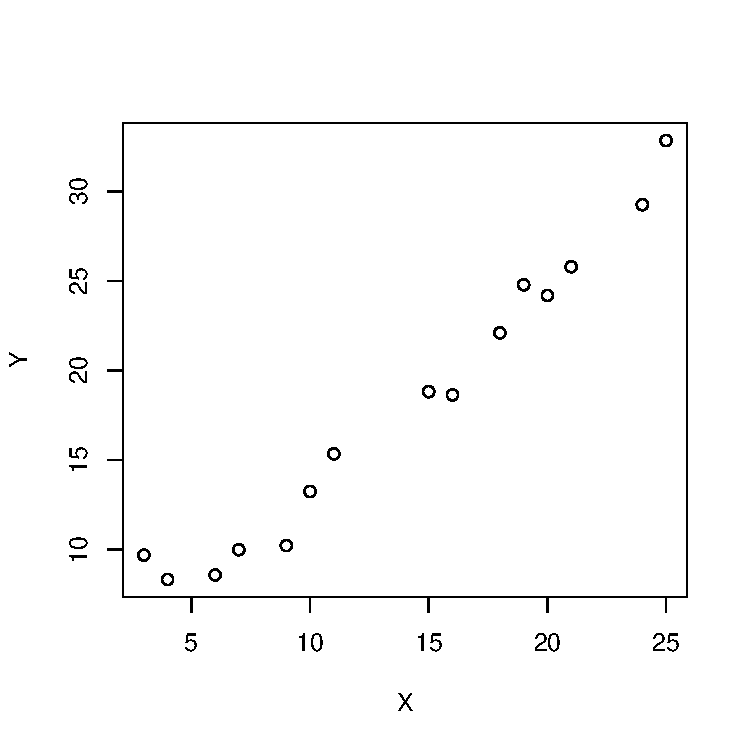
\includegraphics[width=.45\linewidth]{figure/fig-unnamed-chunk-39-1} 

}



\end{knitrout}
      \caption{Graphique des données de l'exercice
        \ref{chap:multiple}.\ref{ex:multiple:quadratique}}
      \label{fig:multiple:quadratique}
    \end{figure}
    Par la suite, on peut estimer les paramètres de ce modèle avec la
    fonction \texttt{lm} de \textsf{R}:
\begin{knitrout}
\definecolor{shadecolor}{rgb}{0.969, 0.969, 0.969}\color{fgcolor}\begin{kframe}
\begin{alltt}
\hlstd{fit} \hlkwb{<-} \hlkwd{lm}\hlstd{(Y} \hlopt{~} \hlkwd{poly}\hlstd{(X,} \hlnum{2}\hlstd{),} \hlkwc{data} \hlstd{= donnees)}
\hlkwd{summary}\hlstd{(fit)}
\end{alltt}
\begin{verbatim}
## 
## Call:
## lm(formula = Y ~ poly(X, 2), data = donnees)
## 
## Residuals:
##     Min      1Q  Median      3Q     Max 
## -1.9123 -0.6150 -0.1905  0.6367  1.6921 
## 
## Coefficients:
##             Estimate Std. Error t value Pr(>|t|)    
## (Intercept)  18.1240     0.3025   59.91 3.10e-16 ***
## poly(X, 2)1  29.6754     1.1717   25.33 8.72e-12 ***
## poly(X, 2)2   4.0899     1.1717    3.49  0.00446 ** 
## ---
## Signif. codes:  
## 0 '***' 0.001 '**' 0.01 '*' 0.05 '.' 0.1 ' ' 1
## 
## Residual standard error: 1.172 on 12 degrees of freedom
## Multiple R-squared:  0.982,	Adjusted R-squared:  0.979 
## F-statistic: 326.8 on 2 and 12 DF,  p-value: 3.434e-11
\end{verbatim}
\begin{alltt}
\hlkwd{anova}\hlstd{(fit)}
\end{alltt}
\begin{verbatim}
## Analysis of Variance Table
## 
## Response: Y
##            Df Sum Sq Mean Sq F value    Pr(>F)    
## poly(X, 2)  2 897.36  448.68  326.79 3.434e-11 ***
## Residuals  12  16.48    1.37                      
## ---
## Signif. codes:  
## 0 '***' 0.001 '**' 0.01 '*' 0.05 '.' 0.1 ' ' 1
\end{verbatim}
\end{kframe}
\end{knitrout}
    Tant le test $F$ global que les tests $t$ individuels sont
    concluants, le coefficient de détermination est élevé et l'on peut
    constater à la figure \ref{fig:multiple:quadratique2} que
    l'ajustement du modèle est bon. On conclut donc qu'un modèle
    adéquat pour cet ensemble de données est
    \begin{displaymath}
      Y_t = 18,12 +
      29,68 X_t +
      4,09 X_t^2 + \varepsilon_t, \quad
      \varepsilon_t \sim N(0, 1,373).
    \end{displaymath}
    \begin{figure}
      \centering
\begin{knitrout}
\definecolor{shadecolor}{rgb}{0.969, 0.969, 0.969}\color{fgcolor}\begin{kframe}
\begin{alltt}
\hlkwd{plot}\hlstd{(Y} \hlopt{~} \hlstd{X,} \hlkwc{data} \hlstd{= donnees)}
\hlstd{x} \hlkwb{<-} \hlkwd{seq}\hlstd{(}\hlkwd{min}\hlstd{(donnees}\hlopt{$}\hlstd{X),} \hlkwd{max}\hlstd{(donnees}\hlopt{$}\hlstd{X),} \hlkwc{length} \hlstd{=} \hlnum{200}\hlstd{)}
\hlkwd{lines}\hlstd{(x,} \hlkwd{predict}\hlstd{(fit,} \hlkwd{data.frame}\hlstd{(}\hlkwc{X} \hlstd{= x),} \hlkwc{lwd} \hlstd{=} \hlnum{2}\hlstd{))}
\end{alltt}
\end{kframe}

{\centering 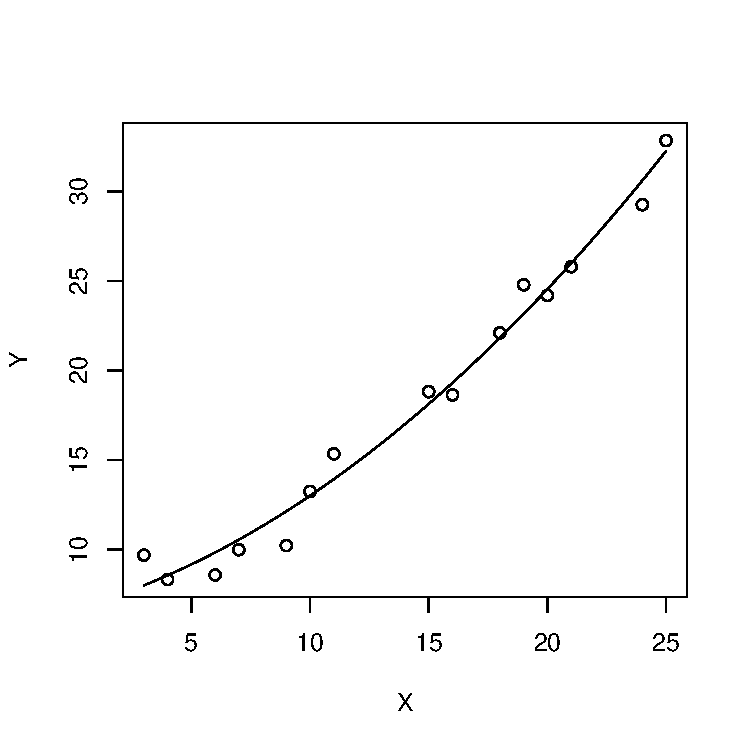
\includegraphics[width=.45\linewidth]{figure/fig-unnamed-chunk-41-1} 

}



\end{knitrout}
      \caption{Graphique des données de l'exercice
        \ref{chap:multiple}.\ref{ex:multiple:quadratique} et courbe
        obtenue par régression}
      \label{fig:multiple:quadratique2}
    \end{figure}
  \end{sol}
\end{exercice}

\begin{exercice}
  \label{ex:multiple:pondere}
  On vous donne les 23 données dans le tableau ci-dessous.
  \begin{center}
    \begin{tabular}{rcc@{\qquad}rcc@{\qquad}rcc}
      \toprule
      $t$ & $Y_t$ & $X_t$ & $t$ & $Y_t$ & $X_t$ & $t$ & $Y_t$ & $X_t$ \\
      \midrule
      12 & 2,3 & 1,3 & 19 & 1,7 & 3,7 &  6 & 2,8 & 5,3 \\
      23 & 1,8 & 1,3 & 20 & 2,8 & 4,0 & 10 & 2,1 & 5,3 \\
      7 & 2,8 & 2,0 &  5 & 2,8 & 4,0 &  4 & 3,4 & 5,7 \\
      8 & 1,5 & 2,0 &  2 & 2,2 & 4,0 &  9 & 3,2 & 6,0 \\
      17 & 2,2 & 2,7 & 21 & 3,2 & 4,7 & 13 & 3,0 & 6,0 \\
      22 & 3,8 & 3,3 & 15 & 1,9 & 4,7 & 14 & 3,0 & 6,3 \\
      1 & 1,8 & 3,3 & 18 & 1,8 & 5,0 & 16 & 5,9 & 6,7 \\
      11 & 3,7 & 3,7 &  3 & 3,5 & 5,3 \\
      \bottomrule
    \end{tabular}
  \end{center}
  \begin{enumerate}
  \item Calculer l'estimateur des moindres carrés ordinaires
    $\betabh$.
  \item Supposons que la variance de $Y_{16}$ est $4 \sigma^2$ plutôt
    que $\sigma^2$. Recalculer la régression en a) en utilisant cette
    fois les moindres carrés pondérés.
  \item Refaire la partie b) en supposant maintenant que la variance
    de l'observation $Y_{16}$ est $16 \sigma^2$. Quelles différences
    note-t-on?
  \end{enumerate}

  \begin{rep}
    \begin{inparaenum}
    \item $\betabh = (%
      1,4256,
      0,3158)$
    \item $\betabh^* = (%
      1,7213,
      0,2243)$
    \item $\betabh^* = (%
      1,808,
      0,1975)$
    \end{inparaenum}
  \end{rep}
  \begin{sol}
    Comme on peut le constater à la figure \ref{fig:multiple:pondere},
    le point $(X_{16}, Y_{16})$ est plus éloigné des autres. En b) et
    c), on diminue son poids dans la régression.
    \begin{figure}
      \centering
\begin{knitrout}
\definecolor{shadecolor}{rgb}{0.969, 0.969, 0.969}\color{fgcolor}\begin{kframe}
\begin{alltt}
\hlkwd{plot}\hlstd{(Y} \hlopt{~} \hlstd{X,} \hlkwc{data} \hlstd{= donnees)}
\hlkwd{points}\hlstd{(donnees}\hlopt{$}\hlstd{X[}\hlnum{16}\hlstd{], donnees}\hlopt{$}\hlstd{Y[}\hlnum{16}\hlstd{],} \hlkwc{pch} \hlstd{=} \hlnum{16}\hlstd{)}
\end{alltt}
\end{kframe}

{\centering 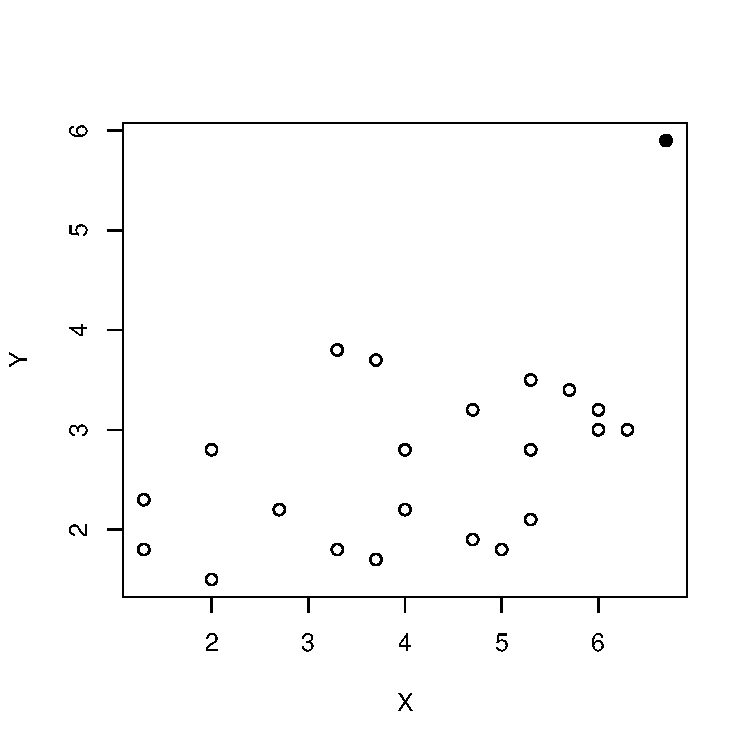
\includegraphics[width=.45\linewidth]{figure/fig-unnamed-chunk-43-1} 

}



\end{knitrout}
      \caption{Graphique des données de l'exercice
        \ref{chap:multiple}.\ref{ex:multiple:pondere}. Le cercle plein
        représente la donnée $(X_{16}, Y_{16})$.}
      \label{fig:multiple:pondere}
    \end{figure}
    \begin{enumerate}
    \item On calcule d'abord l'estimateur des moindres carrés ordinaires:
\begin{knitrout}
\definecolor{shadecolor}{rgb}{0.969, 0.969, 0.969}\color{fgcolor}\begin{kframe}
\begin{alltt}
\hlstd{(fit1} \hlkwb{<-} \hlkwd{lm}\hlstd{(Y} \hlopt{~} \hlstd{X,} \hlkwc{data} \hlstd{= donnees))}
\end{alltt}
\begin{verbatim}
## 
## Call:
## lm(formula = Y ~ X, data = donnees)
## 
## Coefficients:
## (Intercept)            X  
##      1.4256       0.3158
\end{verbatim}
\end{kframe}
\end{knitrout}
    \item Si l'on suppose que la variance de la données $(X_{16},
      Y_{16})$ est quatre fois plus élevée que la variance des autres
      données, alors il convient d'accorder un point quatre fois moins
      grand à cette donnée dans la régression. Cela requiert les
      moindres carrés pondérés. Pour calculer les estimateurs avec
      \texttt{lm} dans \textsf{R}, on utilise l'argument
      \texttt{weights}:
\begin{knitrout}
\definecolor{shadecolor}{rgb}{0.969, 0.969, 0.969}\color{fgcolor}\begin{kframe}
\begin{alltt}
\hlstd{w} \hlkwb{<-} \hlkwd{rep}\hlstd{(}\hlnum{1}\hlstd{,} \hlkwd{nrow}\hlstd{(donnees))}
\hlstd{w[}\hlnum{16}\hlstd{]} \hlkwb{<-} \hlnum{0.25}
\hlstd{(fit2} \hlkwb{<-} \hlkwd{update}\hlstd{(fit1,} \hlkwc{weights} \hlstd{= w))}
\end{alltt}
\begin{verbatim}
## 
## Call:
## lm(formula = Y ~ X, data = donnees, weights = w)
## 
## Coefficients:
## (Intercept)            X  
##      1.7213       0.2243
\end{verbatim}
\end{kframe}
\end{knitrout}
    \item On répète la procédure en b) avec un poids de encore plus
      petit pour la donnée $(X_{16}, Y_{16})$:
\begin{knitrout}
\definecolor{shadecolor}{rgb}{0.969, 0.969, 0.969}\color{fgcolor}\begin{kframe}
\begin{alltt}
\hlstd{w[}\hlnum{16}\hlstd{]} \hlkwb{<-} \hlnum{0.0625}
\hlstd{(fit3} \hlkwb{<-} \hlkwd{update}\hlstd{(fit1,} \hlkwc{weights} \hlstd{= w))}
\end{alltt}
\begin{verbatim}
## 
## Call:
## lm(formula = Y ~ X, data = donnees, weights = w)
## 
## Coefficients:
## (Intercept)            X  
##      1.8080       0.1975
\end{verbatim}
\end{kframe}
\end{knitrout}
      Plus le poids accordé à la donnée $(X_{16}, Y_{16})$ est faible,
      moins la droite de régression est attirée vers ce point (voir la
      figure \ref{fig:multiple:pondere2}).
      \begin{figure}[t]
        \centering
\begin{knitrout}
\definecolor{shadecolor}{rgb}{0.969, 0.969, 0.969}\color{fgcolor}\begin{kframe}
\begin{alltt}
\hlkwd{plot}\hlstd{(Y} \hlopt{~} \hlstd{X,} \hlkwc{data} \hlstd{= donnees)}
\hlkwd{points}\hlstd{(donnees}\hlopt{$}\hlstd{X[}\hlnum{16}\hlstd{], donnees}\hlopt{$}\hlstd{Y[}\hlnum{16}\hlstd{],} \hlkwc{pch} \hlstd{=} \hlnum{16}\hlstd{)}
\hlkwd{abline}\hlstd{(fit1,} \hlkwc{lwd} \hlstd{=} \hlnum{2}\hlstd{,} \hlkwc{lty} \hlstd{=} \hlnum{1}\hlstd{)}
\hlkwd{abline}\hlstd{(fit2,} \hlkwc{lwd} \hlstd{=} \hlnum{2}\hlstd{,} \hlkwc{lty} \hlstd{=} \hlnum{2}\hlstd{)}
\hlkwd{abline}\hlstd{(fit3,} \hlkwc{lwd} \hlstd{=} \hlnum{2}\hlstd{,} \hlkwc{lty} \hlstd{=} \hlnum{3}\hlstd{)}
\hlkwd{legend}\hlstd{(}\hlnum{1.2}\hlstd{,} \hlnum{6}\hlstd{,} \hlkwc{legend} \hlstd{=} \hlkwd{c}\hlstd{(}\hlstr{"Modèle a)"}\hlstd{,} \hlstr{"Modèle b)"}\hlstd{,} \hlstr{"Modèle c)"}\hlstd{),}
       \hlkwc{lwd} \hlstd{=} \hlnum{2}\hlstd{,} \hlkwc{lty} \hlstd{=} \hlnum{1}\hlopt{:}\hlnum{3}\hlstd{)}
\end{alltt}
\end{kframe}

{\centering 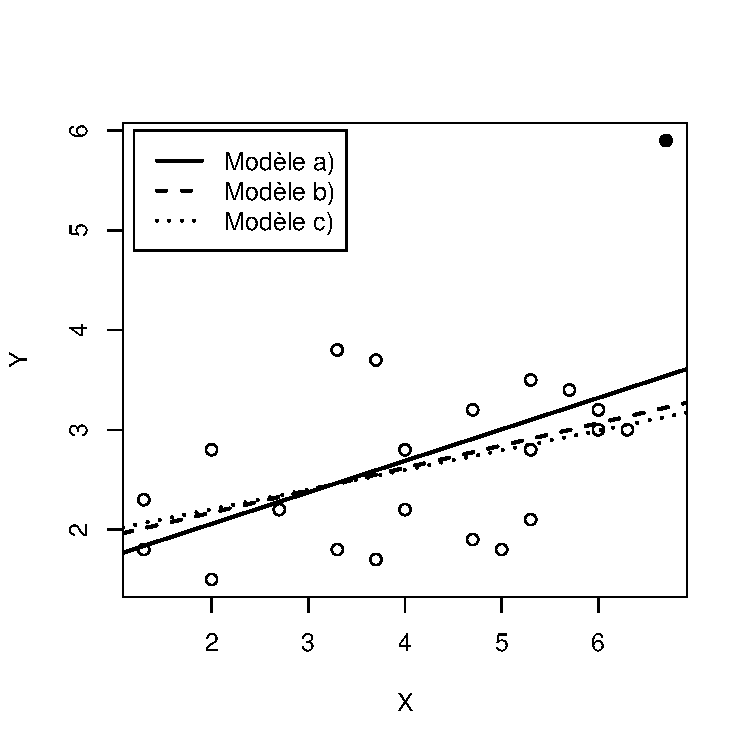
\includegraphics[width=.45\linewidth]{figure/fig-unnamed-chunk-47-1} 

}



\end{knitrout}
        \caption{Graphique des données de l'exercice
          \ref{chap:multiple}.\ref{ex:multiple:pondere} avec les
          droites de régression obtenues à l'aide des moindres carrés
          pondérés.}
        \label{fig:multiple:pondere2}
      \end{figure}
    \end{enumerate}
  \end{sol}
\end{exercice}

\begin{exercice}
  \label{ex:multiple:taxi}
  Une coopérative de taxi new-yorkaise s'intéresse à la consommation
  de carburant des douze véhicules de sa flotte en fonction de leur
  âge.  Hormis leur âge, les véhicules sont identiques et utilisent
  tous le même type d'essence. La seule chose autre différence notable
  d'un véhicule à l'autre est le sexe du conducteur: la coopérative
  emploie en effet des hommes et des femmes. La coopérative a
  recueilli les données suivantes afin d'établir un modèle de
  régression pour la consommation de carburant:
  \begin{center}
    \begin{tabular}{ccc}
      \toprule
      Consommation (mpg) & Âge du véhicule & Sexe du conducteur \\
      \midrule
      12,3 & 3 & M \\
      12,0 & 4 & F \\
      13,7 & 3 & F \\
      14,2 & 2 & M \\
      15,5 & 1 & F \\
      11,1 & 5 & M \\
      10,6 & 4 & M \\
      14,0 & 1 & M \\
      16,0 & 1 & F \\
      13,1 & 2 & M \\
      14,8 & 2 & F \\
      10,2 & 5 & M \\
      \bottomrule
    \end{tabular}
  \end{center}
  \begin{enumerate}
  \item En plaçant les points sur un graphique de la consommation de
    carburant en fonction de l'âge du véhicule, identifier s'il existe
    ou non une différence entre la consommation de carburant des
    femmes et celle des hommes. \emph{Astuce}: utiliser un symbole
    (\texttt{pch}) différent pour chaque groupe.
  \item Établir un modèle de régression pour la consommation de
    carburant. Afin de pouvoir intégrer la variable qualitative «sexe
    du conducteur» dans le modèle, utiliser une variable indicatrice
    du type
    \begin{displaymath}
      X_{t2} =
      \begin{cases}
        1, & \text{si le conducteur est un homme} \\
        0, & \text{si le conducteur est une femme}.
      \end{cases}
    \end{displaymath}
  \item Quelle est, selon le modèle établi en b), la consommation
    moyenne d'une voiture taxi de quatre ans conduite par une femme?
    Fournir un intervalle de confiance à 90~\% pour cette prévision.
  \end{enumerate}

  \begin{rep}
    \begin{inparaenum}
      \stepcounter{enumi}
    \item $\text{mpg} = %
      16,687
      -1,04 \text{ age}
      -1,206 \text{ sexe}$
    \item $12,53 \pm
      0,58 \text{ mpg}$
    \end{inparaenum}
  \end{rep}
  \begin{sol}
    \begin{enumerate}
    \item Voir la figure \ref{fig:multiple:taxi} pour le graphique. Il
      y a effectivement une différence entre la consommation de
      carburant des hommes et des femmes: ces dernières font plus de
      milles avec un gallon d'essence.
      \begin{figure}
        \centering
\begin{knitrout}
\definecolor{shadecolor}{rgb}{0.969, 0.969, 0.969}\color{fgcolor}\begin{kframe}
\begin{alltt}
\hlstd{hommes} \hlkwb{<-} \hlkwd{subset}\hlstd{(donnees, sexe} \hlopt{==} \hlstr{"M"}\hlstd{)}
\hlstd{femmes} \hlkwb{<-} \hlkwd{subset}\hlstd{(donnees, sexe} \hlopt{==} \hlstr{"F"}\hlstd{)}
\hlkwd{plot}\hlstd{(mpg} \hlopt{~} \hlstd{age,} \hlkwc{data} \hlstd{= hommes,}
     \hlkwc{xlim} \hlstd{=} \hlkwd{range}\hlstd{(donnees}\hlopt{$}\hlstd{age),} \hlkwc{ylim} \hlstd{=} \hlkwd{range}\hlstd{(donnees}\hlopt{$}\hlstd{mpg))}
\hlkwd{points}\hlstd{(mpg} \hlopt{~} \hlstd{age,} \hlkwc{data} \hlstd{= femmes,} \hlkwc{pch} \hlstd{=} \hlnum{16}\hlstd{)}
\hlkwd{legend}\hlstd{(}\hlnum{4}\hlstd{,} \hlnum{16}\hlstd{,} \hlkwc{legend} \hlstd{=} \hlkwd{c}\hlstd{(}\hlstr{"Hommes"}\hlstd{,} \hlstr{"Femmes"}\hlstd{),} \hlkwc{pch} \hlstd{=} \hlkwd{c}\hlstd{(}\hlnum{1}\hlstd{,} \hlnum{16}\hlstd{))}
\end{alltt}
\end{kframe}

{\centering 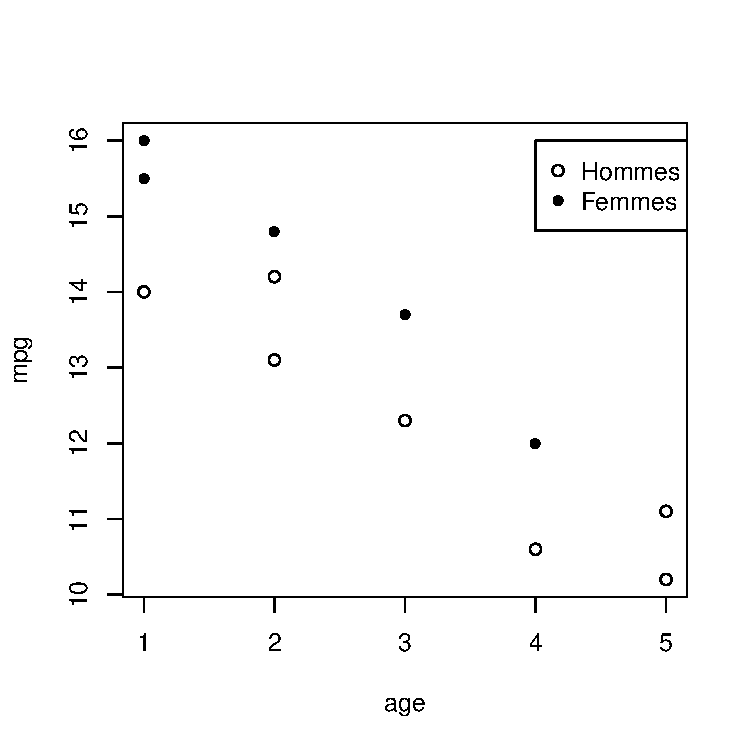
\includegraphics[width=.45\linewidth]{figure/fig-unnamed-chunk-49-1} 

}



\end{knitrout}
        \caption{Graphique des données de l'exercice
          \ref{chap:multiple}.\ref{ex:multiple:taxi}}
        \label{fig:multiple:taxi}
      \end{figure}
    \item Remarquer que la variable \texttt{sexe} est un facteur et peut
      être utilisée telle quelle dans \texttt{lm}:
\begin{knitrout}
\definecolor{shadecolor}{rgb}{0.969, 0.969, 0.969}\color{fgcolor}\begin{kframe}
\begin{alltt}
\hlstd{(fit} \hlkwb{<-} \hlkwd{lm}\hlstd{(mpg} \hlopt{~} \hlstd{age} \hlopt{+} \hlstd{sexe,} \hlkwc{data} \hlstd{= donnees))}
\end{alltt}
\begin{verbatim}
## 
## Call:
## lm(formula = mpg ~ age + sexe, data = donnees)
## 
## Coefficients:
## (Intercept)          age        sexeM  
##      16.687       -1.040       -1.206
\end{verbatim}
\end{kframe}
\end{knitrout}
    \item Calcul d'une prévision pour la valeur moyenne de la variable
      \texttt{mpg}:
\begin{knitrout}
\definecolor{shadecolor}{rgb}{0.969, 0.969, 0.969}\color{fgcolor}\begin{kframe}
\begin{alltt}
\hlkwd{predict}\hlstd{(fit,} \hlkwc{newdata} \hlstd{=} \hlkwd{data.frame}\hlstd{(}\hlkwc{age} \hlstd{=} \hlnum{4}\hlstd{,} \hlkwc{sexe} \hlstd{=} \hlstr{"F"}\hlstd{),}
        \hlkwc{interval} \hlstd{=} \hlstr{"confidence"}\hlstd{,} \hlkwc{level} \hlstd{=} \hlnum{0.90}\hlstd{)}
\end{alltt}
\begin{verbatim}
##        fit      lwr      upr
## 1 12.52876 11.94584 13.11168
\end{verbatim}
\end{kframe}
\end{knitrout}
    \end{enumerate}
  \end{sol}
\end{exercice}

\begin{exercice}
Le modèle de régression linéaire multiple $$Y_i=\beta_0+\beta_1 x_{i1}+\beta_2 x_{i2}+\beta_3 x_{i3}+\varepsilon_i, \mbox{ pour }i=1,...,n$$ a été ajusté à des données avec la méthode des moindres carrés.

\begin{enumerate}
\item La figure~\ref{fig:multiple:postulat1} montre le QQ-plot des résidus studentisés. À la lumière de ce graphique, y a-t-il un postulat du modèle qui n'est pas vérifié? Si oui, lequel et pourquoi? S'il y a lieu, expliquer l'impact de la violation de ce postulat. 

\bigskip
\item La figure~\ref{fig:multiple:postulat2} montre les résidus studentisés en fonction de chacune des variables exogènes et en fonction des valeurs prédites. Utiliser ces graphiques pour commenter sur la validité des postulats du modèle. Y en a-t-il qui ne sont pas respectés? S'il y a lieu, expliquer l'impact de la violation de ce ou ces postulats. 

\end{enumerate}

\begin{figure}
\centering \caption{QQ-Plot des résidus studentisés}\label{fig:multiple:postulat1}
\centerline{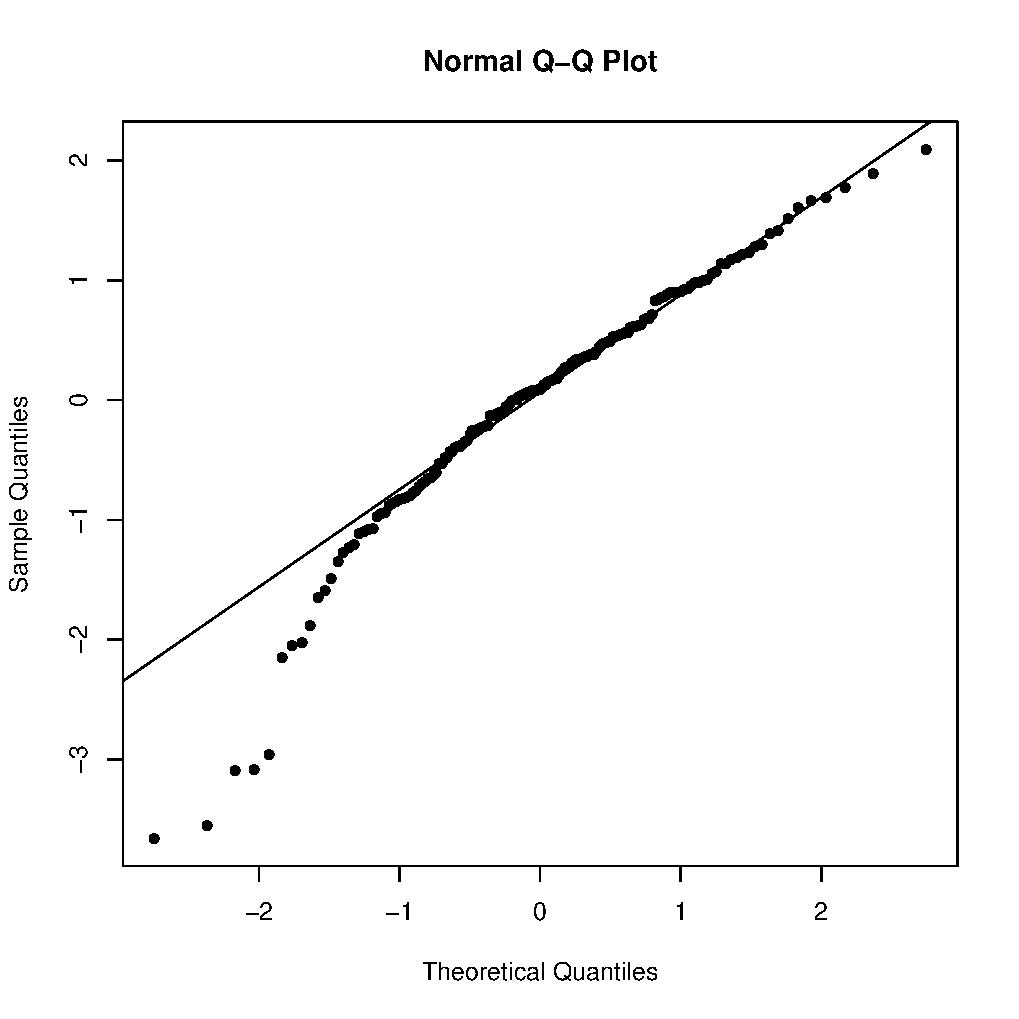
\includegraphics[width=0.6\textwidth]{figure/QQPlotLifeExp-c.pdf}}
\end{figure}

\begin{figure}
\centering \caption{Nuage de points des résidus studentisés en fonction de chacune des variables exogènes et en fonction de la variable prédite}\label{fig:multiple:postulat2}
\centerline{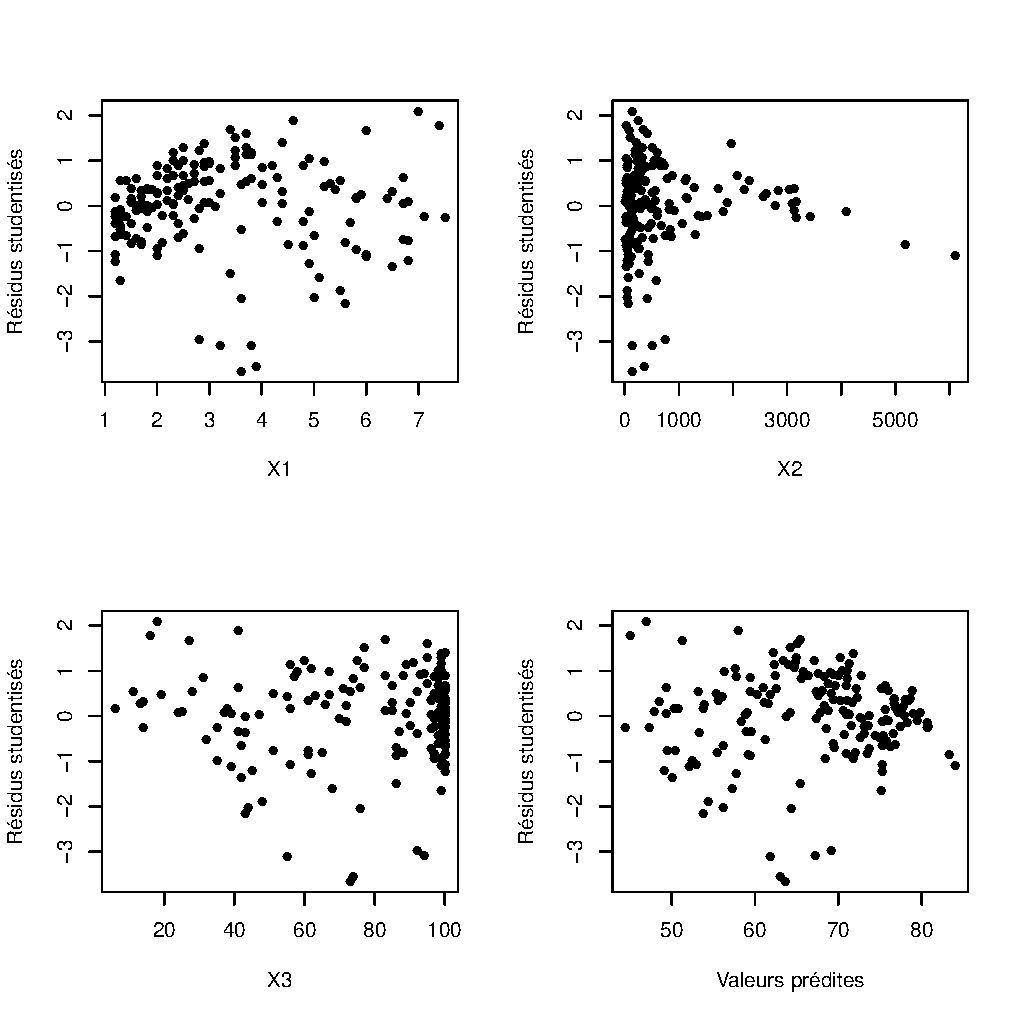
\includegraphics[width=14cm]{figure/ResPlots.pdf}}
\end{figure}

\begin{sol}
\begin{enumerate}
\item Le postulat de normalité semble violé.

La distribution des résidus a une queue inférieure plus épaisse que la loi normale, ce que l'on voit à gauche du Q-Q plot, puisque les poits ne sont pas alignés.

Le postulat de normalité n'est pas critique, parce que les estimateurs des moindres carrés ont un sens quand même. Toutefois, les tests d'hypothèses et les intervalles de confiance ne sont pas valides.

\item Le graphique des résidus en fonction de $x_2$ montre que le postulat de linéarité semble violé. Cela implique que le modèle n'est pas valide.

On observe de l'hétéroscédasticité (par exemple, dans les graphiques 1, 3 ou 4) puisque les résidus ne semblent pas avoir une variance constante. 

Cela signifie que les variances des paramètres ne sont pas calculées de façon appropriée OU il faudrait effectuer une transformation sur les variables pour régler ces problèmes.


\end{enumerate}
\end{sol}
\end{exercice}

\begin{exercice}
La base de données \texttt{OutlierExample.csv} disponible sur le site du cours contient 19 observations de base, et trois observations supplémentaires, notées par les \texttt{CODES} 1, 2 et 3, qui sont aberrantes ou influentes.

\begin{enumerate}
\item Importez la base de données et tracez un nuage de points de \texttt{Y} en fonction de \texttt{X}.
\item Roulez les lignes de code suivantes pour observer le graphique avec les 3 points ajoutés
\begin{verbatim}
library(ggplot2)
ggplot(dat, aes(x= X, y= Y, label=CODES))+
  geom_point() +
  geom_text(aes(label=ifelse(CODES>0,CODES,'')),hjust=0,vjust=0)
\end{verbatim}

\item Ajustez un modèle linéaire en incluant seulement les 19 points dont le code est 0. Regardez l'ajustement et commentez.
\item Ajustez un modèle linéaire en incluant les 19 points dont le code est 0 et le point de code 1. Quel est l'impact de l'inclusion de ce point sur le $R^2$ et sur les estimations des paramètres? Étudiez le résultat de la fonction \texttt{influence.measures()}.
\item Ajustez un modèle linéaire en incluant les 19 points dont le code est 0 et le point de code 2. Quel est l'impact de l'inclusion de ce point sur le $R^2$ et sur les estimations des paramètres? Étudiez le résultat de la fonction \texttt{influence.measures()}.
\item Ajustez un modèle linéaire en incluant les 19 points dont le code est 0 et le point de code 3. Quel est l'impact de l'inclusion de ce point sur le $R^2$ et sur les estimations des paramètres? Étudiez le résultat de la fonction \texttt{influence.measures()}.
\end{enumerate}

\begin{sol}
On pourrait croire qu'un point sur 20, ça ne change rien, mais ce n'est pas le cas! Le point 1 a un impact sur la pente et la qualité de l'ajustement. Le point 2 a un grand levier mais n'affecte pas beaucoup les estimations, le point 3 a un grand levier et un gros impact.

\begin{verbatim}
dat <- read.csv("OutlierExample.csv")

dim(dat)

summary(dat)

library(ggplot2)

ggplot(dat, aes(x= X, y= Y, label=CODES))+
  geom_point() +
  geom_text(aes(label=ifelse(CODES>0,CODES,'')),hjust=0,vjust=0)

fit0 <- lm(Y~X,dat,subset=(CODES==0))
summary(fit0)
plot(dat[,1:2],pch=16)
points(dat[match(1:3,dat$CODES),1:2],col=2:4,pch=16:18,cex=1.2)
abline(fit0)

fit1 <- lm(Y~X,dat,subset=(CODES<=1))
summary(fit1)
abline(fit1,col=2,lty=2)

fit2 <- lm(Y~X,dat,subset=(CODES%in%c(0,2)))
summary(fit2)
abline(fit2,col=3,lty=3)

fit3 <- lm(Y~X,dat,subset=(CODES%in%c(0,3)))
summary(fit3)
abline(fit3,col=4,lty=4)

influence.measures(fit0)
influence.measures(fit1)
influence.measures(fit2)
influence.measures(fit3)

\end{verbatim}
\end{sol}
\end{exercice}

\Closesolutionfile{solutions}
\Closesolutionfile{reponses}

%%%
%%% Insérer les réponses
%%%
\bigskip
\section*{Réponses}

\begin{reponse}{3.2}
    \begin{inparaenum}
      \item $\hat{\beta}_0 = \bar{Y}$
      \item $\hat{\beta}_1 = (\sum_{t=1}^n X_t Y_t)/(\sum_{t=1}^n X_t^2)$
      \end{inparaenum}
  
\end{reponse}
\begin{reponse}{3.6}
    $p \approx 0,01$
  
\end{reponse}
\begin{reponse}{3.7}
    \begin{inparaenum}
    \item $\betabh = (-22,5,\; 6,5,\; 1,5)$
    \item $F = 13,5$, $R^2 = 0,9643$
    \item $t_1 = 3,920$, $t_2 = 1,732$
    \item $13,75 \pm 13,846$
    \end{inparaenum}
  
\end{reponse}
\begin{reponse}{3.8}
    \begin{inparaenum}
      \stepcounter{enumi}
    \item $R^2 = 0,8927$ et
      $F = 145,6$
    \item $12,04 \pm
      2,08$
    \end{inparaenum}
  
\end{reponse}
\begin{reponse}{3.10}
    \begin{inparaenum}
    \item $\mat{y}_{20 \times 1}$, $\mat{X}_{20 \times 4}$, $\betab_{4
        \times 1}$ et $\vepsb_{20 \times 1}$
    \end{inparaenum}
  
\end{reponse}
\begin{reponse}{3.11}
    \begin{inparaenum}
    \item
      \begin{inparaenum}[i)]
      \item 40,44, 3 et 21 degrés de liberté
      \item 0,098, 1 et 21 degrés de liberté
      \item 9,82, 2 et 21 degrés de liberté
      \end{inparaenum}
    \item $X_1$ et $X_3$, ou $X_2$ et $X_3$
    \end{inparaenum}
  
\end{reponse}
\begin{reponse}{3.12}
    $103,67$
  
\end{reponse}
\begin{reponse}{3.15}
    \begin{enumerate}
    \item $\hat{\beta}^* = \sum_{t=1}^n X_t Y_t/\sum_{t=1}^n X_t^2$,
      $\var{\hat{\beta}^*} = \sigma^2/\sum_{t=1}^n X_t^2$
    \item $\hat{\beta}^* = \sum_{t=1}^n w_t X_t Y_t/\sum_{t=1}^n
      w_t X_t^2$,
      $\var{\hat{\beta}^*} = \sigma^2/\sum_{t=1}^n w_t X_t^2$
    \item $\hat{\beta}^* = \bar{Y}/\bar{X}$,
      $\var{\hat{\beta}^*} = \sigma^2/(n \bar{X})$
    \item $\hat{\beta}^* = \sum_{t=1}^n Y_t/X_t$,
      $\var{\hat{\beta}^*} = \sigma^2/n$
    \end{enumerate}
  
\end{reponse}
\begin{reponse}{3.16}
    $Y_t = 18,12 +
    29,68 X_t +
    4,09 X_t^2 + \varepsilon_t$,
    $\varepsilon_t \sim N(0, 1,373)$
  
\end{reponse}
\begin{reponse}{3.17}
    \begin{inparaenum}
    \item $\betabh = (%
      1,4256,
      0,3158)$
    \item $\betabh^* = (%
      1,7213,
      0,2243)$
    \item $\betabh^* = (%
      1,808,
      0,1975)$
    \end{inparaenum}
  
\end{reponse}
\begin{reponse}{3.18}
    \begin{inparaenum}
      \stepcounter{enumi}
    \item $\text{mpg} = %
      16,687
      -1,04 \text{ age}
      -1,206 \text{ sexe}$
    \item $12,53 \pm
      0,58 \text{ mpg}$
    \end{inparaenum}
  
\end{reponse}



%%% Local Variables:
%%% mode: latex
%%% TeX-master: "exercices_methodes_statistiques"
%%% End:

%<<child='selection.Rnw'>>=
%@
%
%\part{Modèles linéaires généralisés}
%
%<<child='glm.Rnw'>>=
%@
%
%<<child='comptage.Rnw'>>=
%@

\part{Annexes}
\appendix
%<<child='regression.Rnw'>>=
%@
%\chapter{Éléments d'algèbre matricielle}
\label{chap:elements}

Cette annexe présente quelques résultats d'algèbre matricielle utiles
en régression linéaire.

\section{Trace}

La \emph{trace} d'une matrice est la somme des éléments de la diagonale.

\begin{thm}
  \label{thm:elements:trace}
  Soient $\mat{A} = [a_{ij}]$ et $\mat{B} = [b_{ij}]$ des matrices
  carrées $k \times k$. Alors
  \begin{enumerate}[a)]
  \item $\tr(\mat{A}) = \sum_{i=1}^k a_{ii}$
  \item $\tr(\mat{A} + \mat{B}) = \tr(\mat{A}) + \tr(\mat{B})$.
  \end{enumerate}
\end{thm}

\begin{thm}
  \label{thm:elements:symetrie_trace}
  Soient les matrices $\mat{A}_{p \times q}$ et $\mat{B}_{q \times
    p}$. Alors $\tr(\mat{AB}) = \tr(\mat{BA})$.
\end{thm}

\enlargethispage{\baselineskip}
\begin{proof}
  Posons $\mat{C} = \mat{AB}$ et $\mat{D} = \mat{BA}$. Par définition
  du produit matriciel, l'élément $c_{ij}$ de la matrice $\mat{C}$ est
  égal au produit scalaire entre la ligne $i$ de $\mat{A}$ et de la
  colonne $j$ de $\mat{B}$, soit
  \begin{displaymath}
    c_{ij} = \sum_{k=1}^q a_{ik} b_{kj}.
  \end{displaymath}
  Les éléments de la diagonale de $\mat{C}$ sont donc $c_{ii} =
  \sum_{j=1}^q a_{ij} b_{ji}$ et, par symétrie, ceux de la diagonale
  de $\mat{D}$ sont $d_{jj} = \sum_{i=1}^p b_{ji} a_{ij}$.  Or,
  \begin{align*}
    \tr(\mat{C})
    &= \sum_{i=1}^p c_{ii} \\
    &= \sum_{i=1}^p \sum_{j=1}^q a_{ij} b_{ji} \\
    &= \sum_{j=1}^q \sum_{i=1}^p b_{ji} a_{ij} \\
    &= \sum_{j=1}^p d_{jj} \\
    &= \tr(\mat{D}).
  \end{align*}
\end{proof}


\section{Formes quadratiques et dérivées}

Soit $\mat{A} = [a_{ij}]$ une matrice $k \times k$ symétrique et
$\mat{x} = (x_1, \dots, x_k)^\prime$ un vecteur. Alors
\begin{displaymath}
  \mat{x^\prime A x} = \sum_{i=1}^k \sum_{j=1}^k a_{ij} x_i x_j
\end{displaymath}
est une forme quadratique.

Par exemple, si
\begin{displaymath}
  \mat{x} =
  \begin{bmatrix}
    x_1 \\
    x_2
  \end{bmatrix}
  \quad
  \text{et}
  \quad
  \mat{A} =
  \begin{bmatrix}
    a_{11} & a_{12} \\
    a_{12} & a_{22}
  \end{bmatrix},
\end{displaymath}
alors
\begin{align*}
  \mat{x^\prime Ax}
  &= \sum_{i=1}^2 \sum_{j=1}^2 a_{ij} x_i x_j \\
  &= a_{11} x_1^2 + 2 a_{12} x_1 x_2 + a_{22} x_2^2.
\end{align*}

\begin{rem}
  Si $\mat{A}$ est diagonale, $\mat{x^\prime Ax} = \sum_{i=1}^k a_{ii} x_i^2$.
\end{rem}

\begin{thm}
  \label{thm:elements:derivee_produit_scalaire}
  Soient $\mat{x} = (x_1, \dots, x_k)^\prime$ et $\mat{a} = (a_1,
  \dots, a_k)^\prime$, d'où $\mat{x^\prime a} = a_1 x_1 + \dots + a_k x_k =
  \sum_{i=1}^k a_i x_i$. Alors
  \begin{align*}
    \frac{d}{d \mat{x}}\, \mat{x^\prime a}
    &= \frac{d}{d \mat{x}} \sum_{i=1}^k a_i x_i \\
    &=
    \begin{bmatrix}
      \frac{d}{d x_1}\, \sum_{i=1}^k a_i x_i \\
      \vdots \\
      \frac{d}{d x_k}\, \sum_{i=1}^k a_i x_i
    \end{bmatrix} \\
    &=
    \begin{bmatrix}
      a_1 \\
      \vdots \\
      a_k
    \end{bmatrix} \\
    &= \mat{a}.
  \end{align*}
\end{thm}

\begin{thm}
  \label{thm:elements:derivee_forme_quadratique}
  Soit $\mat{A}_{k \times k}$ une matrice symétrique. Alors
  \begin{displaymath}
    \frac{d}{d \mat{x}}\, \mat{x^\prime A x} = 2 \mat{A x}.
  \end{displaymath}
\end{thm}

\begin{proof}
  On a
  \begin{align*}
    \mat{x^\prime A x}
    &= \sum_{i=1}^k \sum_{j=1}^k a_{ij} x_i x_j \\
    &= \sum_{i=1}^k a_{ii} x_i^2 +
       \sum_{i=1}^k \sum_{\overset{j=1}{j \neq i}}^k a_{ij} x_i x_j.
  \end{align*}
  Par conséquent, pour $t = 1, \dots, k$ et puisque $a_{ij} = a_{ji}$,
  \begin{align*}
    \frac{\partial}{\partial x_t}\, \mat{x^\prime A x}
    &= 2 a_{tt} x_t + \sum_{\overset{i=1}{i \neq t}}^k a_{it} x_i +
       \sum_{\overset{j=1}{j \neq t}}^k a_{tj} x_j \\
    &= 2 \sum_{i=1}^k a_{it} x_t, \\
    \intertext{d'où}
    \frac{d}{d \mat{x}}\, \mat{x^\prime A x}
    &= 2 \mat{A x}.
  \end{align*}
\end{proof}

\begin{thm}
  \label{thm:elements:derivee_fonction}
  Si $f(\mat{x})$ est une fonction quelconque du vecteur $\mat{x}$, alors
  \begin{displaymath}
    \frac{d}{d \mat{x}}\, f(\mat{x})^\prime \mat{A} f(\mat{x}) =
    2 \left( \frac{d}{d \mat{x}} f(\mat{x}) \right)^\prime \mat{A} f(\mat{x}).
  \end{displaymath}
\end{thm}

Vérifier en exercice les résultats ci-dessus pour une matrice
$\mat{A}$ $3 \times 3$.


\section{Vecteurs et matrices aléatoires}

Soit $X_1, \dots, X_n$ des variables aléatoires. Alors
\begin{displaymath}
  \mat{x} =
  \begin{bmatrix}
    X_1 \\
    \vdots \\
    X_n
  \end{bmatrix}
\end{displaymath}
est un \emph{vecteur aléatoire}. On définit le vecteur espérance
\begin{align*}
  \esp{\mat{x}}
  &=
  \begin{bmatrix}
    \esp{X_1} \\
    \vdots \\
    \esp{X_n}
  \end{bmatrix}
\end{align*}
et la matrice de variance-covariance
\begin{align*}
  \varmat{\mat{x}}
  &= \esp{(\mat{x} - \esp{\mat{x}})(\mat{x} - \esp{\mat{x}})^\prime } \\
  &=
  \begin{bmatrix}
    \var{X_1} & \dots & \Cov(X_1, X_n) \\
    \vdots    & \ddots & \vdots \\
    \Cov(X_n, X_1) & \dots & \var{X_n}
  \end{bmatrix}
\end{align*}

\begin{thm}
  \label{thm:elements:esp_var}
  Soit $\mat{x}$ un vecteur aléatoire et $\mat{A}$ une matrice de
  constantes. Alors
  \begin{enumerate}[a)]
  \item $\esp{\mat{Ax}} = \mat{A} \esp{\mat{x}}$
    \label{thm:elements:esp_var:esp}
  \item $\varmat{\mat{Ax}} = \mat{A} \varmat{\mat{x}} \mat{A}^\prime $.
    \label{thm:elements:esp_var:var}
  \end{enumerate}
\end{thm}

\begin{proof}[Démonstration de b)]
  \begin{align*}
    \varmat{\mat{Ax}}
    &= \esp{(\mat{Ax} - \esp{\mat{Ax}})(\mat{Ax} - \esp{\mat{Ax}})^\prime } \\
    &= \esp{\mat{A}(\mat{x} - \esp{\mat{x}})(\mat{x} - \esp{\mat{x}})^\prime
       \mat{A}^\prime } \\
    &= \mat{A} \varmat{\mat{x}} \mat{A}^\prime .
  \end{align*}
\end{proof}

\begin{exemple}
  Soit $\mat{A} = [1\; 1]$, $\mat{x}^\prime = [X_1\; X_2]$ et $Y =
  \mat{Ax}$, donc $Y = X_1 + X_2$. Alors
  \begin{align*}
    \esp{Y}
    &= \mat{A} \esp{\mat{x}} \\
    &= [1\:\: 1]
    \begin{bmatrix}
    \esp{X_1} \\
    \esp{X_2}
    \end{bmatrix} \\
    &= \esp{X_1} + \esp{X_2}
    \intertext{et}
    \varmat{Y}
    &= \mat{A} \varmat{\mat{x}} \mat{A}^\prime \\
    &= [1\:\: 1]
    \begin{bmatrix}
      \var{X_1} & \Cov(X_1, X_2) \\
      \Cov(X_2, X_1) & \var{X_2}
    \end{bmatrix}
    \begin{bmatrix}
      1 \\
      1
    \end{bmatrix} \\
    &= \var{X_1} + \var{X_2} + 2\, \Cov(X_1, X_2).
  \end{align*}
\end{exemple}

%%% Local Variables:
%%% mode: latex
%%% TeX-master: "exercices_methodes_statistiques"
%%% End:

\chapter{Solutions}
\label{chap:solutions}

\section*{Chapitre \ref{chap:simple}}
\addcontentsline{toc}{section}{Chapitre \protect\ref{chap:simple}}

\begin{solution}{2.1}
    \begin{enumerate}
    \item Voir la figure \ref{fig:simple:base}. Remarquer que l'on
      peut, dans la fonction \texttt{plot}, utiliser une formule pour
      exprimer la relation entre les variables.
      \begin{figure}
\begin{knitrout}
\definecolor{shadecolor}{rgb}{0.969, 0.969, 0.969}\color{fgcolor}\begin{kframe}
\begin{alltt}
\hlstd{x}\hlkwb{<-}\hlkwd{c}\hlstd{(}\hlnum{65}\hlstd{,} \hlnum{43}\hlstd{,} \hlnum{44}\hlstd{,} \hlnum{59}\hlstd{,} \hlnum{60}\hlstd{,} \hlnum{50}\hlstd{,} \hlnum{52}\hlstd{,} \hlnum{38}\hlstd{,} \hlnum{42}\hlstd{,} \hlnum{40}\hlstd{)}
\hlstd{y}\hlkwb{<-}\hlkwd{c}\hlstd{(}\hlnum{12}\hlstd{,} \hlnum{32}\hlstd{,} \hlnum{36}\hlstd{,} \hlnum{18}\hlstd{,} \hlnum{17}\hlstd{,} \hlnum{20}\hlstd{,} \hlnum{21}\hlstd{,} \hlnum{40}\hlstd{,} \hlnum{30}\hlstd{,} \hlnum{24}\hlstd{)}
\hlkwd{plot}\hlstd{(y} \hlopt{~} \hlstd{x,} \hlkwc{pch} \hlstd{=} \hlnum{16}\hlstd{)}
\end{alltt}
\end{kframe}

{\centering 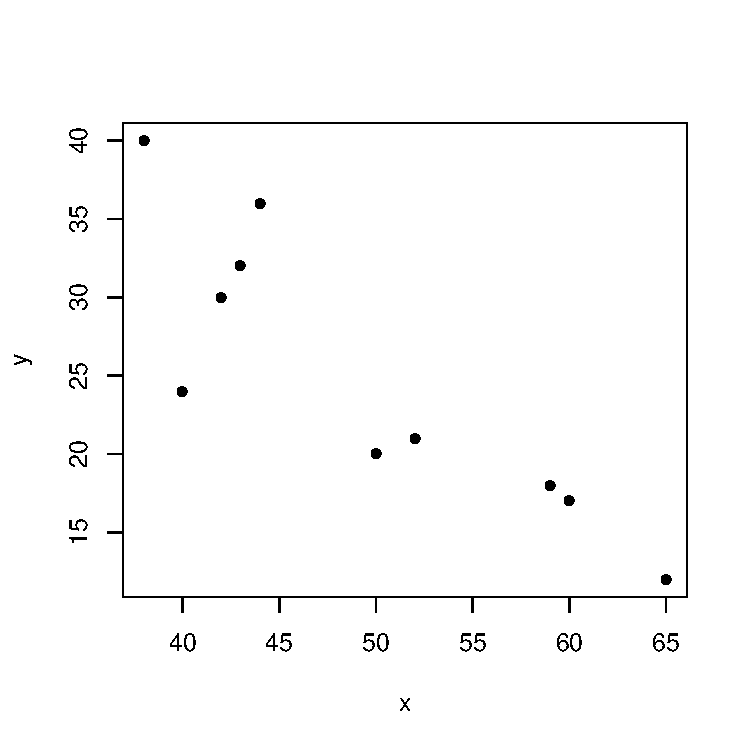
\includegraphics[width=.45\linewidth]{figure/fig-simple-base-1}

}



\end{knitrout}
        \caption{Relation entre les données de l'exercice
          \ref{chap:simple}.\ref{ex:simple:base}}
        \label{fig:simple:base}
      \end{figure}
    \item Les équations normales sont les équations à résoudre pour
      trouver les estimateurs de $\beta_0$ et $\beta_1$ minimisant la
      somme des carrés
      \begin{align*}
        S(\beta_0, \beta_1)
        &=\sum_{t = 1}^n \varepsilon^2_t \\
        &=\sum_{t = 1}^n \left(Y_t-\beta_0-\beta_1X_t\right)^2.
      \end{align*}
      Or,
      \begin{align*}
        \frac{\partial S}{\partial \beta_0}
        &= -2 \sum_{t=1}^n (Y_t - \beta_0 - \beta_1 X_t) \\
        \frac{\partial S}{\partial \beta_1}
        &= -2 \sum_{t=1}^n (Y_t - \beta_0 - \beta_1 X_t) X_t,
      \end{align*}
      d'où les équations normales sont
      \begin{align*}
        \sum_{t=1}^n (Y_t - \hat{\beta}_0 - \hat{\beta}_1 X_t) &= 0 \\
        \sum_{t=1}^n (Y_t - \hat{\beta}_0 - \hat{\beta}_1 X_t) X_t &= 0.
      \end{align*}
    \item Par la première des deux équations normales, on trouve
      \begin{displaymath}
        \sum_{t=1}^nY_t-n\hat{\beta}_0-\hat{\beta}_1\sum_{t=1}^nX_t = 0,
      \end{displaymath}
      soit, en isolant $\hat{\beta}_0$,
      \begin{displaymath}
        \hat{\beta}_0=\frac{\sum_{t=1}^nY_t-\hat{\beta}_1\sum_{t=1}^nX_t}{n}=\bar{Y}-\hat{\beta}_1\bar{X}.
      \end{displaymath}
      De la seconde équation normale, on obtient
      \begin{displaymath}
        \sum_{t=1}^n X_t Y_t -
        \hat{\beta}_0 \sum_{t=1}^n X_t -
        \hat{\beta}_1 \sum_{t=1}^n X_t^2 = 0
      \end{displaymath}
      puis, en remplaçant $\hat{\beta}_0$ par la valeur obtenue ci-dessus,
      \begin{displaymath}
        \hat{\beta}_1
        \left(
          \sum_{t=1}^n X_t^2 - n \bar{X}^2
        \right) =
        \sum_{t=1}^n X_t Y_t - n \bar{X} \bar{Y}.
      \end{displaymath}
      Par conséquent,
      \begin{align*}
        \hat{\beta}_1
        &= \frac{\sum_{t=1}^n X_t Y_t - n \bar{X}\bar{Y}}{\sum_{t=1}^n
          X_t^2 - n \bar{X}^2} \\
        &= \frac{\nombre{11654} - (10)(49,3)(25)}{\nombre{25103} -
          (10)(49,3)^2} \\
        &= -0,8407 \\
        \intertext{et}
        \hat{\beta}_0
        &=\bar{Y}-\hat{\beta}_1\bar{X}\\
        &=25 - (-0,8407)(49,3)\\
        &=66,4488.
      \end{align*}
    \item On peut calculer les prévisions correspondant à $X_1, \dots,
      X_{10}$ --- ou valeurs ajustées --- à partir de la relation
      $\hat{Y}_t = 66,4488 - 0,8407 X_t$, $t = 1, 2, \dots, 10$. Avec
      \textsf{R}, on crée un objet de type modèle de régression avec
      \texttt{lm} et on en extrait les valeurs ajustées avec
      \texttt{fitted}:
\begin{knitrout}
\definecolor{shadecolor}{rgb}{0.969, 0.969, 0.969}\color{fgcolor}\begin{kframe}
\begin{alltt}
\hlstd{fit} \hlkwb{<-} \hlkwd{lm}\hlstd{(y} \hlopt{~} \hlstd{x)}
\hlkwd{fitted}\hlstd{(fit)}
\end{alltt}
\begin{verbatim}
##        1        2        3        4        5        6
## 11.80028 30.29670 29.45596 16.84476 16.00401 24.41148
##        7        8        9       10
## 22.72998 34.50044 31.13745 32.81894
\end{verbatim}
\end{kframe}
\end{knitrout}
      Pour ajouter la droite de régression au graphique de la figure
      \ref{fig:simple:base}, il suffit d'utiliser la fonction
      \texttt{abline} avec en argument l'objet créé avec
      \texttt{lm}. L'ordonnée à l'origine et la pente de la droite
      seront extraites automatiquement. Voir la figure \ref{fig:simple:base2}.
      \begin{figure}
        \centering
\begin{knitrout}
\definecolor{shadecolor}{rgb}{0.969, 0.969, 0.969}\color{fgcolor}\begin{kframe}
\begin{alltt}
\hlkwd{abline}\hlstd{(fit)}
\end{alltt}
\end{kframe}
\end{knitrout}
\begin{knitrout}
\definecolor{shadecolor}{rgb}{0.969, 0.969, 0.969}\color{fgcolor}

{\centering \includegraphics[width=.45\linewidth]{figure/fig-unnamed-chunk-5-1}

}



\end{knitrout}
        \caption{Relation entre les données de l'exercice
          \ref{chap:simple}.\ref{ex:simple:base} et la droite de
          régression}
        \label{fig:simple:base2}
      \end{figure}
    \item Les résidus de la régression sont $e_t = Y_t - \hat{Y}_t$,
      $t = 1, \dots, 10$. Dans \textsf{R}, la fonction
      \texttt{residuals} extrait les résidus du modèle:
\begin{knitrout}
\definecolor{shadecolor}{rgb}{0.969, 0.969, 0.969}\color{fgcolor}\begin{kframe}
\begin{alltt}
\hlkwd{residuals}\hlstd{(fit)}
\end{alltt}
\begin{verbatim}
##          1          2          3          4          5
##  0.1997243  1.7032953  6.5440421  1.1552437  0.9959905
##          6          7          8          9         10
## -4.4114773 -1.7299837  5.4995615 -1.1374514 -8.8189450
\end{verbatim}
\end{kframe}
\end{knitrout}
      On vérifie ensuite que la somme des résidus est
      (essentiellement) nulle:
\begin{knitrout}
\definecolor{shadecolor}{rgb}{0.969, 0.969, 0.969}\color{fgcolor}\begin{kframe}
\begin{alltt}
\hlkwd{sum}\hlstd{(}\hlkwd{residuals}\hlstd{(fit))}
\end{alltt}
\begin{verbatim}
## [1] -4.440892e-16
\end{verbatim}
\end{kframe}
\end{knitrout}
    \end{enumerate}
  
\end{solution}
\begin{solution}{2.2}
    \begin{enumerate}
    \item Nous avons le modèle de régression usuel. Les coefficients
      de la régression sont
      \begin{align*}
        \hat{\beta}_1
        &=\frac{\sum_{t=1}^8 X_tY_t-n\bar{X}\bar{Y}}{\sum_{t=1}^8
          X_t^2-n\bar{X}^2} \\
        &=\frac{146-(8)(32/8)(40/8)}{156-(8)(32/8)^2}  \\
        &=-0,5 \\
        \intertext{et}
        \hat{\beta}_0
        &=\bar{Y}-\hat{\beta}_1\bar{X} \\
        &=(40/8)-(-0,5)(32/8) \\
        &=7.
      \end{align*}
    \item Les sommes de carrés sont
      \begin{align*}
        \SST
        &=\sum_{t=1}^8(Y_t-\bar{Y})^2 \\
        &=\sum_{t=1}^8Y_t^2-n\bar{Y}^2 \\
        &=214-(8)(40/8)^2 \\
        &=14, \\
        \SSR
        &=\sum_{t=1}^8(\hat{Y}_t-\bar{Y})^2 \\
        &=\sum_{t=1}^8\hat{\beta}_1^2(X_t-\bar{X})^2 \\
        &=\hat{\beta}_1^2(\sum_{t=1}^8X_t^2-n\bar{X}^2) \\
        &=(-1/2)^2(156-(8)(32/8)^2) \\
        &=7.
      \end{align*}
      et $\SSE = \SST - \SSR = 14 - 7 = 7$. Par conséquent, $R^2 =
      SSR/SST = 7/14 = 0,5$, donc la régression explique 50~\% de la
      variation des $Y_t$ par rapport à leur moyenne $\bar{Y}$. Le
      tableau ANOVA est le suivant:
      \begin{center}
        \begin{tabular}{lcccc}
          \toprule
          Source & SS & d.l. & MS & Ratio F \\
          \midrule
          Régression & 7 & 1 & 7   & 6 \\
          Erreur     & 7 & 6 & 7/6 &  \\
          \midrule
          Total & 14 & 7 & & \\
          \bottomrule
        \end{tabular}
      \end{center}
    \end{enumerate}
  
\end{solution}
\begin{solution}{2.3}
    \begin{enumerate}
    \item Voir la figure \ref{fig:simple:women}.
      \begin{figure}
        \centering
\begin{knitrout}
\definecolor{shadecolor}{rgb}{0.969, 0.969, 0.969}\color{fgcolor}\begin{kframe}
\begin{alltt}
\hlkwd{data}\hlstd{(women)}
\hlkwd{plot}\hlstd{(weight} \hlopt{~} \hlstd{height,} \hlkwc{data} \hlstd{= women,} \hlkwc{pch} \hlstd{=} \hlnum{16}\hlstd{)}
\end{alltt}
\end{kframe}

{\centering \includegraphics[width=.45\linewidth]{figure/fig-unnamed-chunk-9-1}

}



\end{knitrout}
        \caption{Relation entre la taille et le poids moyen de femmes américaines âgées de 30 à 39 ans (données \texttt{women})}
        \label{fig:simple:women}
      \end{figure}
    \item Le graphique montre qu'un modèle linéaire serait
      excellent. On estime les paramètres de ce modèle avec \texttt{lm}:
\begin{knitrout}
\definecolor{shadecolor}{rgb}{0.969, 0.969, 0.969}\color{fgcolor}\begin{kframe}
\begin{alltt}
\hlstd{(fit} \hlkwb{<-} \hlkwd{lm}\hlstd{(weight} \hlopt{~} \hlstd{height,} \hlkwc{data} \hlstd{= women))}
\end{alltt}
\begin{verbatim}
##
## Call:
## lm(formula = weight ~ height, data = women)
##
## Coefficients:
## (Intercept)       height
##      -87.52         3.45
\end{verbatim}
\end{kframe}
\end{knitrout}
    \item Voir la figure \ref{fig:simple:women2}.
      \begin{figure}
        \centering
\begin{knitrout}
\definecolor{shadecolor}{rgb}{0.969, 0.969, 0.969}\color{fgcolor}\begin{kframe}
\begin{alltt}
\hlkwd{abline}\hlstd{(fit)}
\end{alltt}
\end{kframe}
\end{knitrout}
\begin{knitrout}
\definecolor{shadecolor}{rgb}{0.969, 0.969, 0.969}\color{fgcolor}

{\centering \includegraphics[width=.45\linewidth]{figure/fig-unnamed-chunk-12-1}

}



\end{knitrout}
        \caption{Relation entre les données \texttt{women} et droite de régression linéaire simple}
        \label{fig:simple:women2}
      \end{figure}
      On constate que l'ajustement est excellent.
    \item Le résultat de la fonction \texttt{summary} appliquée au
      modèle \texttt{fit} est le suivant:
\begin{knitrout}
\definecolor{shadecolor}{rgb}{0.969, 0.969, 0.969}\color{fgcolor}\begin{kframe}
\begin{alltt}
\hlkwd{summary}\hlstd{(fit)}
\end{alltt}
\begin{verbatim}
##
## Call:
## lm(formula = weight ~ height, data = women)
##
## Residuals:
##     Min      1Q  Median      3Q     Max
## -1.7333 -1.1333 -0.3833  0.7417  3.1167
##
## Coefficients:
##              Estimate Std. Error t value Pr(>|t|)
## (Intercept) -87.51667    5.93694  -14.74 1.71e-09 ***
## height        3.45000    0.09114   37.85 1.09e-14 ***
## ---
## Signif. codes:
## 0 '***' 0.001 '**' 0.01 '*' 0.05 '.' 0.1 ' ' 1
##
## Residual standard error: 1.525 on 13 degrees of freedom
## Multiple R-squared:  0.991,	Adjusted R-squared:  0.9903
## F-statistic:  1433 on 1 and 13 DF,  p-value: 1.091e-14
\end{verbatim}
\end{kframe}
\end{knitrout}
      Le coefficient de détermination est donc
      $R^2 = 0,991$, %$
      ce qui est près de 1 et confirme donc l'excellent
      ajustement du modèle évoqué en c).
    \item On a
\begin{knitrout}
\definecolor{shadecolor}{rgb}{0.969, 0.969, 0.969}\color{fgcolor}\begin{kframe}
\begin{alltt}
\hlkwd{attach}\hlstd{(women)}
\hlstd{SST} \hlkwb{<-} \hlkwd{sum}\hlstd{((weight} \hlopt{-} \hlkwd{mean}\hlstd{(weight))}\hlopt{^}\hlnum{2}\hlstd{)}
\hlstd{SSR} \hlkwb{<-} \hlkwd{sum}\hlstd{((}\hlkwd{fitted}\hlstd{(fit)} \hlopt{-} \hlkwd{mean}\hlstd{(weight))}\hlopt{^}\hlnum{2}\hlstd{)}
\hlstd{SSE} \hlkwb{<-} \hlkwd{sum}\hlstd{((weight} \hlopt{-} \hlkwd{fitted}\hlstd{(fit))}\hlopt{^}\hlnum{2}\hlstd{)}
\hlkwd{all.equal}\hlstd{(SST, SSR} \hlopt{+} \hlstd{SSE)}
\end{alltt}
\begin{verbatim}
## [1] TRUE
\end{verbatim}
\begin{alltt}
\hlkwd{all.equal}\hlstd{(}\hlkwd{summary}\hlstd{(fit)}\hlopt{$}\hlstd{r.squared, SSR}\hlopt{/}\hlstd{SST)}
\end{alltt}
\begin{verbatim}
## [1] TRUE
\end{verbatim}
\end{kframe}
\end{knitrout}
    \end{enumerate}
  
\end{solution}
\begin{solution}{2.4}
    Puisque $\hat{Y}_t = (\bar{Y} - \hat{\beta}_1 \bar{X}) +
    \hat{\beta}_1 X_t = \bar{Y} + \hat{\beta}_1 (X_t - \bar{X})$ et
    que $e_t = Y_t - \hat{Y}_t = (Y_t - \bar{Y}) - \hat{\beta}_1 (X_t
    - \bar{X})$, alors
    \begin{align*}
      \sum_{t = 1}^n (\hat{Y}_t - \bar{Y}) e_t
      &= \hat{\beta}_1
      \left(
        \sum_{t=1}^n (X_t - \bar{X})(Y_t - \bar{Y}) -
        \hat{\beta}_1 \sum_{t = 1}^n (X_t - \bar{X})^2
      \right) \\
      & = \hat{\beta}_1
      \left(
        S_{XY} - \frac{S_{XY}}{S_{XX}}\, S_{XX}
      \right) \\
      & = 0.
    \end{align*}
  
\end{solution}
\begin{solution}{2.5}
    On a un modèle de régression linéaire simple usuel avec $X_t =
    t$. Les estimateurs des moindres carrés des paramètres $\beta_0$ et
    $\beta_1$ sont donc
    \begin{align*}
      \hat{\beta}_0
      &= \bar{Y} - \hat{\beta}_1\, \frac{\sum_{t = 1}^n t}{n} \\
      \intertext{et}
      \hat{\beta}_1
      &= \frac{\sum_{t = 1}^n t Y_t - \bar{Y} \sum_{t = 1}^n t}{\sum_{t
          = 1}^n t^2 - n^{-1} (\sum_{t = 1}^n t)^2}.
    \end{align*}
    Or, puisque $\sum_{t = 1}^n t = n(n + 1)/2$ et $\sum_{t = 1}^n t^2
    = n(n + 1)(2n + 1)/6$, les expressions ci-dessus se simplifient en
    \begin{align*}
      \hat{\beta}_0
      & = \bar{Y} - \hat{\beta}_1\, \frac{n + 1}{2} \\
      \intertext{et}
      \hat{\beta}_1
      & = \frac{\sum_{t=1}^n t Y_t - n(n + 1) \bar{Y}/2}{n(n + 1)(2n +
        1)/6 - n(n + 1)^2/4} \\
      & = \frac{12 \sum_{t=1}^n t Y_t - 6 n (n + 1) \bar{Y}}{n (n^2 - 1)}.
    \end{align*}
  
\end{solution}
\begin{solution}{2.6}
    \begin{enumerate}
    \item L'estimateur des moindres carrés du paramètre $\beta$ est la
      valeur $\hat{\beta}$ minimisant la somme de carrés
      \begin{align*}
        S(\beta)
        &=\sum_{t = 1}^n \varepsilon_t^2 \\
        &=\sum_{t = 1}^n (Y_t - \beta X_t)^2.
      \end{align*}
      Or,
      \begin{displaymath}
        \frac{d}{d \beta}\, S(\beta) = -2 \sum_{t = 1}^n (Y_t -
        \hat{\beta} X_t) X_t,
      \end{displaymath}
      d'où l'unique équation normale de ce modèle est
      \begin{displaymath}
        \sum_{t = 1}^n X_t Y_t - \hat{\beta} \sum_{t=1}^n X_t^2 = 0.
      \end{displaymath}
      L'estimateur des moindres carrés de $\beta$ est donc
      \begin{displaymath}
        \hat{\beta} = \frac{\sum_{t=1}^n X_t Y_t}{\sum_{t=1}^n X_t^2}.
      \end{displaymath}
    \item On doit démontrer que $\esp{\hat{\beta}} = \beta$. On a
      \begin{align*}
        \esp{\hat{\beta}}
        &= \Esp{\frac{\sum_{t=1}^n X_t Y_t}{\sum_{t=1}^n X_t^2}} \\
        &= \frac{1}{\sum_{t=1}^n X_t^2} \sum_{t=1}^n X_t \esp{Y_t} \\
        &= \frac{1}{\sum_{t=1}^nX_t^2} \sum_{t=1}^n X_t \beta X_t \\
        &= \beta\, \frac{\sum_{t=1}^n X_t^2}{\sum_{t=1}^n X_t^2} \\
        &= \beta.
      \end{align*}
    \item Des hypothèses du modèle, on a
      \begin{align*}
        \var{\hat{\beta}}
        &= \Var{\frac{\sum_{t=1}^n X_t Y_t}{\sum_{t=1}^n X_t^2}} \\
        &= \frac{1}{(\sum_{t=1}^n X_t^2)^2} \sum_{t=1}^n X_t^2 \var{Y_t} \\
        &= \frac{\sigma^2}{(\sum_{t=1}^n X_t^2)^2} \sum_{t=1}^n X_t^2 \\
        &= \frac{\sigma^2}{\sum_{t=1}^n X_t^2}.
      \end{align*}
    \end{enumerate}
  
\end{solution}
\begin{solution}{2.7}
    On veut trouver les coefficients $c_1, \dots, c_n$ tels que
    $\esp{\beta^*} = \beta$ et $\var{\beta^*}$ est minimale. On
    cherche donc à minimiser la fonction
    \begin{align*}
      f(c_1, \dots, c_n)
      &= \var{\beta^*} \\
      &= \sum_{t=1}^n c_t^2 \var{Y_t} \\
      &= \sigma^2 \sum_{t=1}^n c_t^2
    \end{align*}
    sous la contrainte $\esp{\beta^*} = \sum_{t=1}^nc_t\esp{Y_t} =
    \sum_{t=1}^nc_t\beta X_t = \beta\sum_{t=1}^nc_tX_t = \beta$, soit
    $\sum_{t=1}^n c_t X_t = 1$ ou $g(c_1, \dots, c_n) = 0$ avec
    \begin{displaymath}
      g(c_1, \dots, c_n) = \sum_{t=1}^n c_t X_t - 1.
    \end{displaymath}
    Pour utiliser la méthode des multiplicateurs de Lagrange, on pose
    \begin{align*}
      \mathcal{L}(c_1, \dots, c_n,\lambda)
      &= f(c_1, \dots, c_n) - \lambda g(c_1, \dots, c_n), \\
      &= \sigma^2 \sum_{t=1}^n c_t^2 - \lambda
      \left(
        \sum_{t=1}^n c_t X_t - 1
      \right),
    \end{align*}
    puis on dérive la fonction $\mathcal{L}$ par rapport à chacune des
    variables $c_1, \dots, c_n$ et $\lambda$. On trouve alors
    \begin{align*}
      \frac{\partial \mathcal{L}}{\partial c_u}
      & = 2 \sigma^2 c_u - \lambda X_u, \quad u = 1, \dots, n \\
      \frac{\partial \mathcal{L}}{\partial \lambda}
      & = - \sum_{t=1}^n c_t X_t + 1.
    \end{align*}
    En posant les $n$ premières dérivées égales à zéro, on obtient
    \begin{displaymath}
      c_t = \frac{\lambda X_t}{2 \sigma^2}.
    \end{displaymath}
    Or, de la contrainte,
    \begin{displaymath}
      \sum_{t=1}^n c_t X_t =
      \frac{\lambda}{2\sigma^2} \sum_{t=1}^n X_t^2 = 1,
    \end{displaymath}
    d'où
    \begin{displaymath}
      \frac{\lambda}{2 \sigma^2} = \frac{1}{\sum_{t=1}^n X_t^2}
    \end{displaymath}
    et, donc,
    \begin{displaymath}
      c_t = \frac{X_t}{\sum_{t=1}^n X_t^2}.
    \end{displaymath}
    Finalement,
    \begin{align*}
      \beta^*
      & = \sum_{t=1}^n c_t Y_t \\
      & = \frac{\sum_{t=1}^n X_t Y_t}{\sum_{t=1}^n X_t^2} \\
      & = \hat{\beta}.
    \end{align*}
  
\end{solution}
\begin{solution}{2.8}
    \begin{enumerate}
    \item Tout d'abord, puisque $\MSE = \SSE/(n - 2) = \sum_{t=1}^n
      (Y_t - \hat{Y}_t)^2/(n - 2)$ et que $\esp{Y_t} =
      \esp{\hat{Y}_t}$, alors
      \begin{align*}
        \esp{MSE}
        &= \frac{1}{n - 2} \Esp{\sum_{t=1}^n (Y_t - \hat{Y}_t)^2} \\
        &= \frac{1}{n - 2} \sum_{t=1}^n \esp{(Y_t - \hat{Y}_t)^2} \\
        &= \frac{1}{n - 2} \sum_{t=1}^n \esp{((Y_t - \esp{Y_t}) -
          (\hat{Y}_t - \esp{\hat{Y}_t}))^2} \\
        &= \frac{1}{n - 2} \sum_{t=1}^n
        \left(
          \var{Y_t} + \var{\hat{Y}_t} - 2\, \Cov(Y_t, \hat{Y}_t)
        \right).
      \end{align*}
      Or, on a par hypothèse du modèle que $\Cov(Y_t, Y_s) =
      \Cov(\varepsilon_t, \varepsilon_s) = \delta_{ts} \sigma^2$, d'où
      $\var{Y_t} = \sigma^2$ et $\var{\bar{Y}} = \sigma^2/n$. D'autre
      part,
      \begin{align*}
        \var{\hat{Y}_t}
        &= \var{\bar{Y} + \hat{\beta}_1 (X_t - \bar{X})} \\
        &= \var{\bar{Y}} + (X_t - \bar{X})^2 \var{\hat{\beta}_1} +
        2 (X_t - \bar{X}) \Cov(\bar{Y}, \hat{\beta}_1)
      \end{align*}
      et l'on sait que
      \begin{align*}
        \var{\hat{\beta}_1}
        &= \frac{\sigma^2}{\sum_{t=1}^n(X_t-\bar{X})^2} \\
        \intertext{et que}
        \Cov(\bar{Y}, \hat{\beta}_1)
        & = \Cov
        \left(
          \frac{\sum_{t = 1}^n Y_t}{n},
          \frac{\sum_{s = 1}^n (X_s - \bar{X}) Y_s}{\sum_{t = 1}^n
            (X_t - \bar{X})^2}
        \right) \\
        &= \frac{1}{n \sum_{t = 1}^n (X_t - \bar{X})^2}
        \sum_{t = 1}^n \sum_{s = 1}^n \Cov(Y_t, (X_s - \bar{X}) Y_s) \\
        &= \frac{1}{n \sum_{t = 1}^n (X_t - \bar{X})^2}
        \sum_{t = 1}^n (X_s - \bar{X}) \var{Y_t} \\
        & = \frac{\sigma^2}{n \sum_{t = 1}^n (X_t - \bar{X})^2}
        \sum_{t = 1}^n (X_t - \bar{X}) \\
        & = 0,
      \end{align*}
      puisque $\sum_{i=1}^n(X_i - \bar{X}) = 0$. Ainsi,
      \begin{displaymath}
        \var{\hat{Y}_t} = \frac{\sigma^2}{n} +
        \frac{(X_t - \bar{X})^2 \sigma^2}{\sum_{t=1}^n (X_t - \bar{X})^2}.
      \end{displaymath}
      De manière similaire, on détermine que
      \begin{align*}
        \Cov(Y_t, \hat{Y}_t)
        &= \Cov(Y_t, \bar{Y} + \hat{\beta}_1 (X_t - \bar{X})) \\
        &= \Cov(Y_t, \bar{Y}) +
        (X_t - \bar{X}) \Cov(Y_t, \hat{\beta}_1) \\
        &= \frac{\sigma^2}{n} + \frac{(X_t -
          \bar{X})^2 \sigma^2}{\sum_{t=1}^n (X_t - \bar{X})^2}.
      \end{align*}
      Par conséquent,
      \begin{align*}
        \esp{(Y_t - \hat{Y}_t)^2}
        &= \frac{n - 1}{n}\, \sigma^2 -
        \frac{(X_t - \bar{X})^2 \sigma^2}{\sum_{t = 1}^n (X_t - \bar{X})^2} \\
        \intertext{et}
        \sum_{t=1}^n \esp{(Y_t - \hat{Y}_t)^2}
        & = (n - 2) \sigma^2,
      \end{align*}
      d'où $\esp{\MSE} = \sigma^2$.
    \item On a
      \begin{align*}
        \esp{\MSR}
        &= \esp{\SSR} \\
        &= \Esp{\sum_{t=1}^n (\hat{Y}_t - \bar{Y})^2} \\
        &= \sum_{t=1}^n \esp{\hat{\beta}_1^2 (X_t - \bar{X})^2} \\
        &= \sum_{t=1}^n (X_t - \bar{X})^2 \esp{\hat{\beta}_1^2} \\
        &= \sum_{t=1}^n (X_t - \bar{X})^2 (\var{\hat{\beta}_1} +
        \esp{\hat{\beta}_1}^2) \\
        &= \sum_{t=1}^n (X_t - \bar{X})^2
        \left(
          \frac{\sigma^2}{\sum_{t=1}^n (X_t - \bar{X})^2} + \beta_1^2
        \right) \\
        &= \sigma^2 + \beta_1^2 \sum_{t=1}^n (X_t - \bar{X})^2.
      \end{align*}
    \end{enumerate}
  
\end{solution}
\begin{solution}{2.9}
    \begin{enumerate}
    \item Il faut exprimer $\hat{\beta}_0^\prime$ et
      $\hat{\beta}_1^\prime$ en fonction de $\hat{\beta}_0$ et
      $\hat{\beta}_1$. Pour ce faire, on trouve d'abord une expression
      pour chacun des éléments qui entrent dans la définition de
      $\hat{\beta}_1^\prime$. Tout d'abord,
      \begin{align*}
        \bar{X}^\prime
        &= \frac{1}{n} \sum_{t=1}^n X_t^\prime \\
        &= \frac{1}{n} \sum_{t=1}^n (c + d X_t) \\
        &= c + d \bar{X},
      \end{align*}
      et, de manière similaire, $\bar{Y}^\prime = a + b \bar{Y}$. Ensuite,
      \begin{align*}
        S_{XX}^\prime
        &= \sum_{t=1}^n (X_t^\prime - \bar{X}^\prime)^2 \\
        &= \sum_{t=1}^n (c + d X_t - c - d \bar{X})^2 \\
        &= d^2 S_{XX}
      \end{align*}
      et $S_{YY}^\prime = b^2 S_{YY}$, $S_{XY}^\prime = bd S_{XY}$.
      Par conséquent,
      \begin{align*}
        \hat{\beta}_1^\prime
        &= \frac{S_{XY}^\prime}{S_{XX}^\prime} \\
        &= \frac{bd S_{XY}}{d^2 S_{XX}} \\
        &= \frac{b}{d}\, \hat{\beta}_1 \\
        \intertext{et}
        \hat{\beta}_0^\prime
        &= \bar{Y}^\prime - \hat{\beta}_1^\prime \bar{X}^\prime \\
        &= a + b \bar{Y} - \frac{b}{d}\, \hat{\beta}_1 (c + d \bar{X}) \\
        &= a - \frac{bc}{d}\, \hat{\beta}_1 + b (\bar{Y} -
        \hat{\beta}_1 \bar{X}) \\
        &= a - \frac{bc}{d}\, \hat{\beta}_1 + b \hat{\beta}_0.
      \end{align*}
    \item Tout d'abord, on établit que
      \begin{align*}
        R^2
        &= \frac{\SSR}{\SST} \\
        &= \frac{\sum_{t=1}^n (\hat{Y_t} - \bar{Y})^2}{\sum_{t=1}^n
          (Y_t - \bar{Y})^2} \\
        &= \hat{\beta}_1^2\, \frac{\sum_{t=1}^n (X_t -
          \bar{X})^2}{\sum_{t=1}^n (Y_t - \bar{Y})^2} \\
        &= \hat{\beta}_1^2\, \frac{S_{XX}}{S_{YY}}.
      \end{align*}
      Maintenant, avec les résultats obtenus en a), on démontre
      directement que
      \begin{align*}
        (R^2)^\prime
        &= (\hat{\beta}_1^\prime)^2 \frac{S_{XX}^\prime}{S_{YY}^\prime} \\
        &=
        \left(
          \frac{b}{d}
        \right)^2\,
        \hat{\beta}_1^2\, \frac{d^2 S_{XX}}{b^2 S_{YY}} \\
        &= \hat{\beta}_1^2\, \frac{S_{XX}}{S_{YY}} \\
        &= R^2.
      \end{align*}
    \end{enumerate}
  
\end{solution}
\begin{solution}{2.10}
    Considérons un modèle de régression usuel avec l'ensemble de
    données $(X_1, Y_1), \dots, (X_n, Y_n), (m \bar{X}, m \bar{Y})$,
    où $\bar{X} = n^{-1} \sum_{t = 1}^n X_t$, $\bar{Y} = n^{-1}
    \sum_{t = 1}^n Y_t$, $m = n/a$ et $a = \sqrt{n + 1} - 1$. On
    définit
    \begin{align*}
      \bar{X}^\prime
      &= \frac{1}{n + 1} \sum_{t = 1}^{n + 1} X_t \\
      &= \frac{1}{n + 1} \sum_{t = 1}^n X_t + \frac{m}{n + 1} \bar{X} \\
      &= k \bar{X} \\
      \intertext{et, de manière similaire,}
      \bar{Y}^\prime
      &= k \bar{Y},
      \intertext{où}
      k
      &= \frac{n + m}{n + 1} \\
      &= \frac{n (a + 1)}{a (n + 1)}.
    \end{align*}
    L'expression pour l'estimateur des moindres carrés de la pente de
    la droite de régression pour cet ensemble de données est
    \begin{align*}
      \hat{\beta}_1
      &= \frac{\sum_{t = 1}^{n + 1} X_t Y_t - (n + 1)
        \bar{X}^\prime \bar{Y}^\prime}{%
        \sum_{t = 1}^{n + 1} X_t^2 - (n + 1) (\bar{X}^\prime)^2} \\
      &= \frac{\sum_{t = 1}^n X_t Y_t + m^2 \bar{X} \bar{Y} - (n + 1)
        k^2 \bar{X} \bar{Y}}{%
        \sum_{t = 1}^n X_t^2 + m^2 \bar{X}^2 - (n + 1) k^2 \bar{X}^2}.
    \end{align*}
    Or,
    \begin{align*}
      m^2 - k^2 (n + 1)
      &= \frac{n^2}{a^2} - \frac{n^2 (a + 1)^2}{a^2 (n + 1)} \\
      &= \frac{n^2 (n + 1) - n^2 (n + 1)}{a^2 (n + 1)} \\
      &= 0.
    \end{align*}
    Par conséquent,
    \begin{align*}
      \hat{\beta}_1
      &= \frac{\sum_{t = 1}^n X_t Y_t}{\sum_{t = 1}^n X_t^2} \\
      &= \hat{\beta}.
    \end{align*}
    Interprétation: en ajoutant un point bien spécifique à n'importe
    quel ensemble de données, on peut s'assurer que la pente de la
    droite de régression sera la même que celle d'un modèle passant
    par l'origine. Voir la figure \ref{fig:simple:pointmagique} pour
    une illustration du phénomène.

    \begin{figure}
      \centering
\begin{knitrout}
\definecolor{shadecolor}{rgb}{0.969, 0.969, 0.969}\color{fgcolor}

{\centering \includegraphics[width=.45\linewidth]{figure/fig-unnamed-chunk-16-1}

}



\end{knitrout}
      \caption{Illustration de l'effet de l'ajout d'un point spécial à
        un ensemble de données. À gauche, la droite de régression
        usuelle. À droite, le même ensemble de points avec le point
        spécial ajouté (cercle plein), la droite de régression avec ce
        nouveau point (ligne pleine) et la droite de régression
        passant par l'origine (ligne pointillée). Les deux droites
        sont parallèles.}
      \label{fig:simple:pointmagique}
    \end{figure}
  
\end{solution}
\begin{solution}{2.11}
    Puisque, selon le modèle, $\varepsilon_t \sim N(0, \sigma^2)$ et
    que $Y_t = \beta_0 + \beta_1 X_t + \varepsilon_t$, alors $Y_t \sim
    N(\beta_0 + \beta_1 X_t, \sigma^2)$. De plus, on sait que
    \begin{align*}
      \hat{\beta}_1
      &= \frac{\sum_{t=1}^n (X_t - \bar{X})(Y_t - \bar{Y})}{%
        \sum_{t=1}^n (X_t - \bar{X})^2} \\
      &= \frac{\sum_{t=1}^n (X_t - \bar{X}) Y_t}{%
        \sum_{t=1}^n (X_t - \bar{X})^2},
    \end{align*}
    donc l'estimateur $\hat{\beta}_1$ est une combinaison linéaire des
    variables aléatoires $Y_1, \dots, Y_n$. Par conséquent,
    $\hat{\beta}_1 \sim N(\esp{\hat{\beta}_1}, \var{\hat{\beta}_1})$,
    où $\esp{\hat{\beta}_1} = \beta_1$ et $\var{\hat{\beta}_1} =
    \sigma^2/S_{XX}$ et, donc,
    \begin{displaymath}
      \Pr
      \left[
        -z_{\alpha/2} <
        \frac{\hat{\beta}_1 - \beta_1}{\sigma/\sqrt{S_{XX}}} <
        z_{\alpha/2}
      \right] = 1 - \alpha.
    \end{displaymath}
    Un intervalle de confiance de niveau $1 - \alpha$ pour le
    paramètre $\beta_1$ lorsque la variance $\sigma^2$ est connue est donc
    \begin{displaymath}
      \beta_1 \in \hat{\beta}_1 \pm z_{\alpha/2}
      \frac{\sigma}{\sqrt{\sum_{t=1}^n (X_t - \bar{X})^2}}.
    \end{displaymath}
  
\end{solution}
\begin{solution}{2.12}
    L'intervalle de confiance pour $\beta_1$ est
    \begin{align*}
      \beta_1
      &\in \hat{\beta}_1 \pm t_{\alpha/2}(n - 2)
      \sqrt{\frac{\hat{\sigma}^2}{S_{XX}}} \\
      &\in \hat{\beta}_1 \pm t_{0,025}(20 - 2) \sqrt{\frac{MSE}{S_{XX}}}.
     \end{align*}
     On nous donne $\SST = S_{YY} = \nombre{20838}$ et $S_{XX} =
     \nombre{10668}$. Par conséquent,
     \begin{align*}
       \SSR
       &= \hat{\beta}_1^2 \sum_{t=1}^{20} (X_t - \bar{X})^2 \\
       &= (-1,104)^2(\nombre{10668}) \\
       &= \nombre{13002,33} \\
       \SSE
       &= \SST - \SSR \\
       &= \nombre{7835,67} \\
       \intertext{et}
       \MSE
       &= \frac{\SSE}{18} \\
       &= 435,315.
     \end{align*}
     De plus, on trouve dans une table de quantiles de la loi de
     Student (ou à l'aide de la fonction \texttt{qt} dans \textsf{R})
     que $t_{0,025}(18) = 2,101$. L'intervalle de confiance recherché
     est donc
     \begin{align*}
       \beta_1
       &\in -1,104 \pm 2,101 \sqrt{\frac{435,315}{\nombre{10668}}} \\
       &\in (-1,528, -0,680).
     \end{align*}
  
\end{solution}
\begin{solution}{2.13}
    \begin{enumerate}
    \item On trouve aisément les estimateurs de la pente et de
      l'ordonnée à l'origine de la droite de régression:
      \begin{align*}
        \hat{\beta}_1
        &= \frac{\sum_{t=1}^n X_t Y_t - n \bar{X}\bar{Y}}{%
          \sum_{t=1}^n X_t^2 - n \bar{X}^2} \\
        &= 1,436 \\
        \hat{\beta}_0
        &= \bar{Y} - \hat{\beta}_1 \bar{X} \\
        &= 9,273.
      \end{align*}
    \item Les sommes de carrés sont
      \begin{align*}
        \SST
        &= \sum_{t=1}^n Y_t^2 - n \bar{Y}^2 \\
        &= 1194 - 11 (9,273)^2 \\
        &= 248,18 \\
        \SSR
        &= \hat{\beta}_1^2
        \left(
          \sum_{t=1}^n X_t^2 - n \bar{X}^2
        \right) \\
        &= (1,436)^2 (110 - 11 (0)) \\
        &= 226,95
      \end{align*}
      et $\SSE = \SST - \SSR = 21,23$. Le tableau d'analyse de
      variance est donc le suivant:

      \begin{center}
        \begin{tabular}{lrrrc}
          \toprule
          Source
          & \multicolumn{1}{c}{SS}
          & \multicolumn{1}{c}{d.l.}
          & \multicolumn{1}{c}{MS}
          & Ratio F \\
          \midrule
          Régression & 226,95 &   1  & 226,95 & 96,21 \\
          Erreur     &  21,23 &   9  &   2,36 &  \\
          \midrule
          Total      & 248,18 &  10  &        & \\
          \bottomrule
        \end{tabular}
      \end{center}

      Or, puisque $t = \sqrt{F} = 9,809 > t_{\alpha/2}(n-2) =
      t_{0,025}(9) = 2,26$, on rejette l'hypothèse $H_0: \beta_1 =
      0$ soit, autrement dit, la pente est significativement
      différente de zéro.
    \item Puisque la variance $\sigma^2$ est inconnue, on l'estime par
      $s^2 = \MSE = 2,36$. On a alors
      \begin{align*}
        \beta_1
        &\in \hat{\beta}_1 \pm t_{\alpha/2}(n-2)
        \sqrt{\widehat{\mathrm{Var}}[\hat{\beta}_1]} \\
        &\in 1,436 \pm 2,26 \sqrt{\frac{2,36}{110}} \\
        &\in (1,105, 1,768).
      \end{align*}
    \item Le coefficient de détermination de la régression est $R^2 =
      \SSR/\SST = 226,95/248,18 = 0,914$, ce qui indique que
      l'ajustement du modèle aux données est très bon. En outre, suite
      au test effectué à la partie b), on conclut que la régression
      est globalement significative.  Toutes ces informations portent
      à conclure qu'il n'y a pas lieu d'utiliser un autre modèle.
    \end{enumerate}
  
\end{solution}
\begin{solution}{2.14}
    On doit déterminer si la régression est significative, ce qui peut
    se faire à l'aide de la statistique $F$. Or, à partir de
    l'information donnée dans l'énoncé, on peut calculer
    \begin{align*}
      \hat{\beta}_1
      &= \frac{\sum_{t=1}^{50} X_t Y_t - 50 \bar{X} \bar{Y}}{%
        \sum_{t=1}^{50} X_t^2 - 50 \bar{X})^2} \\
      &= -0,0110 \\
      \SST
      &= \sum_{t=1}^{50} Y_t^2 - 50 \bar{Y}^2 \\
      &= 78,4098 \\
      \SSR
      &= \hat{\beta}_1^2 \sum_{t=1}^{50} (X_t - \bar{X})^2 \\
      &= 1,1804 \\
      \SSE
      &= \SST - \SSR \\
      &= 77,2294 \\
      \intertext{d'où}
      \MSR
      &= 1,1804 \\
      \MSE
      &= \frac{\SSE}{50 - 2} \\
      &= 1,6089 \\
      \intertext{et, enfin,}
      F
      &= \frac{\MSR}{\MSE} \\
      &= 0,7337.
    \end{align*}
    Soit $F$ une variable aléatoire ayant une distribution de Fisher
    avec 1 et 48 degrés de liberté, soit la même distribution que la
    statistique $F$ sous l'hypothèse $H_0: \beta_1 = 0$. On a que
    $\Pr[F > 0,7337] = 0,3959$, donc la valeur $p$ du test $H_0:
    \beta_1 = 0$ est $0,3959$. Une telle valeur $p$ est généralement
    considérée trop élevée pour rejeter l'hypothèse $H_0$. On ne peut
    donc considérer la relation entre la ligne de vie et l'espérance
    de vie comme significative. (Ou on ne la considère significative
    qu'avec un niveau de confiance de $1 - p = 60,41$~\%.)
  
\end{solution}
\begin{solution}{2.15}
    Premièrement, selon le modèle de régression passant par l'origine,
    $Y_0 = \beta X_0 + \varepsilon_0$ et $\hat{Y}_0 = \hat{\beta}
    X_0$. Considérons, pour la suite, la variable aléatoire $Y_0 -
    \hat{Y}_0$. On voit facilement que $\esp{\hat{\beta}} = \beta$,
    d'où $\esp{Y_0 - \hat{Y}_0} = \esp{\beta X_0 + \varepsilon_0 -
      \hat{\beta} X_0} = \beta X_0 - \beta X_0 = 0$ et
    \begin{displaymath}
      \var{Y_0 - \hat{Y}_0} = \var{Y_0} + \var{\hat{Y}_0} - 2\,
      \Cov(Y_0, \hat{Y}_0).
    \end{displaymath}
    Or, $\Cov(Y_0, \hat{Y}_0) = 0$ par l'hypothèse ii) de l'énoncé,
    $\var{Y_0} = \sigma^2$ et $\var{\hat{Y}_0} = X_0^2\,
    \var{\hat{\beta}}$. De plus,
    \begin{align*}
      \var{\hat{\beta}}
      &= \frac{1}{(\sum_{t=1}^n X_t^2)^2} \sum_{t=1}^n X_t^2\,
      \var{Y_t} \\
      &= \frac{\sigma^2}{\sum_{t=1}^n X_t^2}
    \end{align*}
    d'où, finalement,
    \begin{displaymath}
      \var{Y_0 - \hat{Y}_0} =
      \sigma^2 \left( 1 + \frac{X_0^2}{\sum_{t=1}^n X_t^2} \right).
    \end{displaymath}
    Par l'hypothèse de normalité et puisque $\hat{\beta}$ est une
    combinaison linéaire de variables aléatoires normales,
    \begin{displaymath}
      Y_0 - \hat{Y}_0 \sim N
      \left(
        0, \sigma^2 \left( 1 + \frac{X_0^2}{\sum_{t=1}^n X_t^2} \right)
      \right)
    \end{displaymath}
    ou, de manière équivalente,
    \begin{displaymath}
      \frac{Y_0 - \hat{Y}_0}{\sigma \sqrt{1 + X_0^2/\sum_{t=1}^n X_t^2}}
      \sim N(0, 1).
    \end{displaymath}
    Lorsque la variance $\sigma^2$ est estimée par $s^2$, alors
    \begin{displaymath}
      \frac{Y_0 - \hat{Y}_0}{s \sqrt{1 + X_0^2/\sum_{t=1}^n X_t^2}}
      \sim t(n - 1).
    \end{displaymath}
    La loi de Student a $n - 1$ degrés de liberté puisque le modèle
    passant par l'origine ne compte qu'un seul paramètre. Les bornes
    de l'intervalle de confiance pour la vraie valeur de $Y_0$ sont
    donc
    \begin{displaymath}
      \hat{Y}_0 \pm t_{\alpha/2}(n - 1)\, s\, \sqrt{1 +
        \frac{X_0^2}{\sum_{t=1}^n X_t^2}}.
    \end{displaymath}
  
\end{solution}
\begin{solution}{2.16}
    \begin{enumerate}
    \item Soit $X_1, \dots, X_{10}$ les valeurs de la masse monétaire
      et $Y_1, \dots, Y_{10}$ celles du PNB. On a $\bar{X} = 3,72$,
      $\bar{Y} = 7,55$, $\sum_{t = 1}^{10} X_t^2 = 147,18$, $\sum_{t =
        1}^{10} Y_t^2 = 597,03$ et $\sum_{t = 1}^{10} X_t Y_t =
      295,95$. Par conséquent,
      \begin{align*}
        \hat{\beta}_1
        &= \frac{\sum_{t=1}^{10} X_t Y_t - 10 \bar{X} \bar{Y}}{%
          \sum_{t=1}^{10} X_t^2 - 10 \bar{X}^2} \\
        &= 1,716 \\
        \intertext{et}
        \hat{\beta}_0
        &= \bar{Y} - \hat{\beta}_1 \bar{X} \\
        &= 1,168.
      \end{align*}
      On a donc la relation linéaire $\text{PNB} = 1,168 + 1,716
      \text{ MM}$.
    \item Tout d'abord, on doit calculer l'estimateur $s^2$ de la
      variance car cette quantité entre dans le calcul des intervalles
      de confiance demandés. Pour les calculs à la main, on peut
      éviter de calculer les valeurs de $\hat{Y}_1, \dots,
      \hat{Y}_{10}$ en procédant ainsi:
      \begin{align*}
        \SST
        &= \sum_{t=1}^{10} Y_t^2 - 10 \bar{Y}^2 \\
        &= 27,005 \\
        \SSR
        &= \hat{\beta}_1^2
        \left(
          \sum_{t=1}^{10} X_t^2 - 10 \bar{X}^2
        \right) \\
        &= 25,901,
      \end{align*}
      puis $\SSE = \SST - \SSR = 1,104$ et $s^2 = \MSE = \SSE/(10 - 2)
      = 0,1380$.  On peut maintenant construire les intervalles de
      confiance:
      \begin{align*}
        \beta_0
        &\in \hat{\beta}_0 \pm t_{\alpha/2}(n - 2)\, s\,
        \sqrt{\frac{1}{n} + \frac{\bar{X}^2}{S_{XX}}} \\
        &\in 1,168 \pm (2,306) (0,3715)
        \sqrt{\frac{1}{10} + \frac{3,72^2}{8,796}} \\
        &\in (0,060, 2,276) \\
        \beta_1
        &\in \hat{\beta}_1 \pm t_{\alpha/2}(n - 2)\, s\,
        \sqrt{\frac{1}{S_{XX}}} \\
        &\in 1,716 \pm (2,306) (0,3715) \sqrt{\frac{1}{8,796}} \\
        &\in (1,427, 2,005).
      \end{align*}
      Puisque l'intervalle de confiance pour la pente $\beta_1$ ne
      contient ni la valeur 0, ni la valeur 1, on peut rejeter, avec
      un niveau de confiance de 95~\%, les hypothèses $H_0: \beta_1 =
      0$ et $H_0: \beta_1 = 1$.
    \item Par l'équation obtenue en a) liant le PNB à la masse
      monétaire (MM), un PNB de 12,0 correspond à une masse monétaire
      de
      \begin{align*}
        \text{MM}
        &= \frac{12,0 - 1,168}{1,716} \\
        &= 6,31.
      \end{align*}
    \item On cherche un intervalle de confiance pour la droite de
      régression en $\text{MM}_{1997} = 6,31$ ainsi qu'un intervalle
      de confiance pour la prévision $\text{PNB} = 12,0$ associée à
      cette même valeur de la masse monétaire.  Avec une probabilité
      de $\alpha = 95~\%$, le PNB moyen se trouve dans l'intervalle
      \begin{displaymath}
        12,0 \pm t_{\alpha/2}(n - 2)\, s\,
        \sqrt{\frac{1}{n} + \frac{(6,31 - \bar{X})^2}{S_{XX}}} =
        (11,20, 12,80),
      \end{displaymath}
      alors que la vraie valeur du PNB se trouve dans l'intervalle
      \begin{displaymath}
        12,0 \pm t_{\alpha/2}(n - 2)\, s\,
        \sqrt{1 + \frac{1}{n} + \frac{(6,31 - \bar{X})^2}{S_{XX}}} =
        (10,83, 13,17).
      \end{displaymath}
    \end{enumerate}
  
\end{solution}
\begin{solution}{2.17}
    \begin{enumerate}
    \item Les données du fichier \texttt{house.dat} sont importées
      dans \textsf{R} avec la commande
\begin{knitrout}
\definecolor{shadecolor}{rgb}{0.969, 0.969, 0.969}\color{fgcolor}\begin{kframe}
\begin{alltt}
\hlstd{house} \hlkwb{<-} \hlkwd{read.table}\hlstd{(}\hlstr{"data/house.dat"}\hlstd{,} \hlkwc{header} \hlstd{=} \hlnum{TRUE}\hlstd{)}
\end{alltt}
\end{kframe}
\end{knitrout}
      La figure \ref{fig:simple:house} contient les graphiques de
      \texttt{medv} en fonction de chacune des variables \texttt{rm},
      \texttt{age}, \texttt{lstat} et \texttt{tax}. Le meilleur choix
      de variable explicative pour le prix médian semble être le
      nombre moyen de pièces par immeuble, \texttt{rm}.
      \begin{figure}
        \centering
\begin{knitrout}
\definecolor{shadecolor}{rgb}{0.969, 0.969, 0.969}\color{fgcolor}\begin{kframe}
\begin{alltt}
\hlkwd{par}\hlstd{(}\hlkwc{mfrow} \hlstd{=} \hlkwd{c}\hlstd{(}\hlnum{2}\hlstd{,} \hlnum{2}\hlstd{))}
\hlkwd{plot}\hlstd{(medv} \hlopt{~} \hlstd{rm} \hlopt{+} \hlstd{age} \hlopt{+} \hlstd{lstat} \hlopt{+} \hlstd{tax,} \hlkwc{data} \hlstd{= house,} \hlkwc{ask} \hlstd{=} \hlnum{FALSE}\hlstd{)}
\end{alltt}
\end{kframe}

{\centering \includegraphics[width=.45\linewidth]{figure/fig-unnamed-chunk-19-1}

}



\end{knitrout}
        \caption{Relation entre la variable \texttt{medv} et les
          variables \texttt{rm}, \texttt{age}, \texttt{lstat} et
          \texttt{tax} des données \texttt{house.dat}}
        \label{fig:simple:house}
      \end{figure}
    \item Les résultats ci-dessous ont été obtenus avec \textsf{R}.
\begin{knitrout}
\definecolor{shadecolor}{rgb}{0.969, 0.969, 0.969}\color{fgcolor}\begin{kframe}
\begin{alltt}
\hlstd{fit1} \hlkwb{<-} \hlkwd{lm}\hlstd{(medv} \hlopt{~} \hlstd{rm,} \hlkwc{data} \hlstd{= house)}
\hlkwd{summary}\hlstd{(fit1)}
\end{alltt}
\begin{verbatim}
##
## Call:
## lm(formula = medv ~ rm, data = house)
##
## Residuals:
##     Min      1Q  Median      3Q     Max
## -23.346  -2.547   0.090   2.986  39.433
##
## Coefficients:
##             Estimate Std. Error t value Pr(>|t|)
## (Intercept)  -34.671      2.650  -13.08   <2e-16 ***
## rm             9.102      0.419   21.72   <2e-16 ***
## ---
## Signif. codes:
## 0 '***' 0.001 '**' 0.01 '*' 0.05 '.' 0.1 ' ' 1
##
## Residual standard error: 6.616 on 504 degrees of freedom
## Multiple R-squared:  0.4835,	Adjusted R-squared:  0.4825
## F-statistic: 471.8 on 1 and 504 DF,  p-value: < 2.2e-16
\end{verbatim}
\end{kframe}
\end{knitrout}
      On peut voir que tant l'ordonnée à l'origine que la pente sont
      très significativement différentes de zéro. La régression est
      donc elle-même significative. Cependant, le coefficient de
      détermination n'est que de $R^2 =
      0,4835$, %$
      ce qui indique que d'autres facteurs pourraient expliquer la
      variation dans \texttt{medv}.

      On calcule les bornes de l'intervalle de confiance de la
      régression avec la fonction \texttt{predict}:
\begin{knitrout}
\definecolor{shadecolor}{rgb}{0.969, 0.969, 0.969}\color{fgcolor}\begin{kframe}
\begin{alltt}
\hlstd{pred.ci} \hlkwb{<-} \hlkwd{predict}\hlstd{(fit1,} \hlkwc{interval} \hlstd{=} \hlstr{"confidence"}\hlstd{,} \hlkwc{level} \hlstd{=} \hlnum{0.95}\hlstd{)}
\end{alltt}
\end{kframe}
\end{knitrout}
      La droite de régression et ses bornes d'intervalle de confiance
      inférieure et supérieure sont illustrée à la figure
      \ref{fig:simple:house2}.
      \begin{figure}
        \centering
\begin{knitrout}
\definecolor{shadecolor}{rgb}{0.969, 0.969, 0.969}\color{fgcolor}\begin{kframe}
\begin{alltt}
\hlstd{ord} \hlkwb{<-} \hlkwd{order}\hlstd{(house}\hlopt{$}\hlstd{rm)}
\hlkwd{plot}\hlstd{(medv} \hlopt{~} \hlstd{rm,} \hlkwc{data} \hlstd{= house,} \hlkwc{ylim} \hlstd{=} \hlkwd{range}\hlstd{(pred.ci))}
\hlkwd{matplot}\hlstd{(house}\hlopt{$}\hlstd{rm[ord], pred.ci[ord,],}
        \hlkwc{type} \hlstd{=} \hlstr{"l"}\hlstd{,} \hlkwc{lty} \hlstd{=} \hlkwd{c}\hlstd{(}\hlnum{1}\hlstd{,} \hlnum{2}\hlstd{,} \hlnum{2}\hlstd{),} \hlkwc{lwd}\hlstd{=} \hlnum{2}\hlstd{,}
        \hlkwc{col} \hlstd{=} \hlstr{"black"}\hlstd{,} \hlkwc{add} \hlstd{=} \hlnum{TRUE}\hlstd{)}
\end{alltt}
\end{kframe}

{\centering 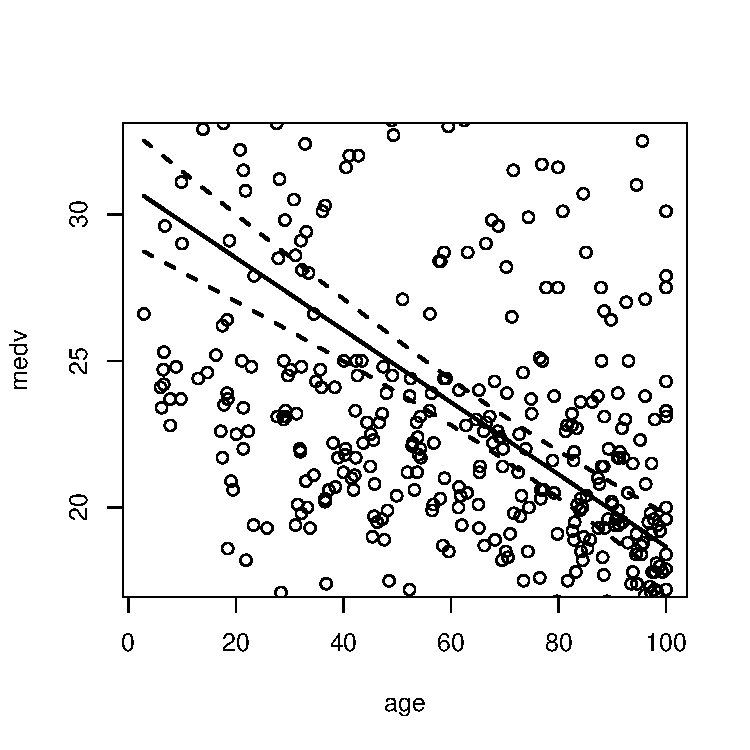
\includegraphics[width=.45\linewidth]{figure/fig-unnamed-chunk-22-1}

}



\end{knitrout}
        \caption{Résultat de la régression de la variable \texttt{rm} sur la variable \texttt{medv} des données \texttt{house.dat}}
        \label{fig:simple:house2}
      \end{figure}
    \item On reprend la même démarche, mais cette fois avec la
      variable \texttt{age}:
\begin{knitrout}
\definecolor{shadecolor}{rgb}{0.969, 0.969, 0.969}\color{fgcolor}\begin{kframe}
\begin{alltt}
\hlstd{fit2} \hlkwb{<-} \hlkwd{lm}\hlstd{(medv} \hlopt{~} \hlstd{age,} \hlkwc{data} \hlstd{= house)}
\hlkwd{summary}\hlstd{(fit2)}
\end{alltt}
\begin{verbatim}
##
## Call:
## lm(formula = medv ~ age, data = house)
##
## Residuals:
##     Min      1Q  Median      3Q     Max
## -15.097  -5.138  -1.958   2.397  31.338
##
## Coefficients:
##             Estimate Std. Error t value Pr(>|t|)
## (Intercept) 30.97868    0.99911  31.006   <2e-16 ***
## age         -0.12316    0.01348  -9.137   <2e-16 ***
## ---
## Signif. codes:
## 0 '***' 0.001 '**' 0.01 '*' 0.05 '.' 0.1 ' ' 1
##
## Residual standard error: 8.527 on 504 degrees of freedom
## Multiple R-squared:  0.1421,	Adjusted R-squared:  0.1404
## F-statistic: 83.48 on 1 and 504 DF,  p-value: < 2.2e-16
\end{verbatim}
\begin{alltt}
\hlstd{pred.ci} \hlkwb{<-} \hlkwd{predict}\hlstd{(fit2,} \hlkwc{interval} \hlstd{=} \hlstr{"confidence"}\hlstd{,} \hlkwc{level} \hlstd{=} \hlnum{0.95}\hlstd{)}
\end{alltt}
\end{kframe}
\end{knitrout}
      La régression est encore une fois très significative. Cependant,
      le $R^2$ est encore plus faible qu'avec la variable
      \texttt{rm}. Les variables \texttt{rm} et \texttt{age}
      contribuent donc chacune à expliquer les variations de la
      variable \texttt{medv} (et \texttt{rm} mieux que \texttt{age}),
      mais aucune ne sait le faire seule de manière satisfaisante. La
      droite de régression et l'intervalle de confiance de celle-ci
      sont reproduits à la figure \ref{fig:simple:house3}. On constate
      que l'intervalle de confiance est plus large qu'en b).
      \begin{figure}
        \centering
\begin{knitrout}
\definecolor{shadecolor}{rgb}{0.969, 0.969, 0.969}\color{fgcolor}\begin{kframe}
\begin{alltt}
\hlstd{ord} \hlkwb{<-} \hlkwd{order}\hlstd{(house}\hlopt{$}\hlstd{age)}
\hlkwd{plot}\hlstd{(medv} \hlopt{~} \hlstd{age,} \hlkwc{data} \hlstd{= house,} \hlkwc{ylim} \hlstd{=} \hlkwd{range}\hlstd{(pred.ci))}
\hlkwd{matplot}\hlstd{(house}\hlopt{$}\hlstd{age[ord], pred.ci[ord,],}
        \hlkwc{type} \hlstd{=} \hlstr{"l"}\hlstd{,} \hlkwc{lty} \hlstd{=} \hlkwd{c}\hlstd{(}\hlnum{1}\hlstd{,} \hlnum{2}\hlstd{,} \hlnum{2}\hlstd{),} \hlkwc{lwd} \hlstd{=} \hlnum{2}\hlstd{,}
        \hlkwc{col} \hlstd{=} \hlstr{"black"}\hlstd{,} \hlkwc{add} \hlstd{=} \hlnum{TRUE}\hlstd{)}
\end{alltt}
\end{kframe}

{\centering \includegraphics[width=.45\linewidth]{figure/fig-unnamed-chunk-24-1}

}



\end{knitrout}
        \caption{Résultat de la régression de la variable \texttt{age} sur la variable \texttt{medv} des données \texttt{house.dat}}
        \label{fig:simple:house3}
      \end{figure}
    \end{enumerate}
  
\end{solution}
\begin{solution}{2.18}
    \begin{enumerate}
    \item On importe les données dans \textsf{R}, puis on effectue les
      conversions demandées. La variable \texttt{consommation}
      contient la consommation des voitures en $\ell$/100~km et la
      variable \texttt{poids} le poids en kilogrammes.
\begin{knitrout}
\definecolor{shadecolor}{rgb}{0.969, 0.969, 0.969}\color{fgcolor}\begin{kframe}
\begin{alltt}
\hlstd{carburant} \hlkwb{<-} \hlkwd{read.table}\hlstd{(}\hlstr{"carburant.dat"}\hlstd{,} \hlkwc{header} \hlstd{=} \hlnum{TRUE}\hlstd{)}
\hlstd{consommation} \hlkwb{<-} \hlnum{235.1954}\hlopt{/}\hlstd{carburant}\hlopt{$}\hlstd{mpg}
\hlstd{poids} \hlkwb{<-} \hlstd{carburant}\hlopt{$}\hlstd{poids} \hlopt{*} \hlnum{0.45455} \hlopt{*} \hlnum{1000}
\end{alltt}
\end{kframe}
\end{knitrout}
    \item La fonction \texttt{summary} fournit l'information
      essentielle pour juger de la validité et de la qualité du
      modèle:
\begin{knitrout}
\definecolor{shadecolor}{rgb}{0.969, 0.969, 0.969}\color{fgcolor}\begin{kframe}
\begin{alltt}
\hlstd{fit} \hlkwb{<-} \hlkwd{lm}\hlstd{(consommation} \hlopt{~} \hlstd{poids)}
\hlkwd{summary}\hlstd{(fit)}
\end{alltt}
\begin{verbatim}
##
## Call:
## lm(formula = consommation ~ poids)
##
## Residuals:
##      Min       1Q   Median       3Q      Max
## -2.07123 -0.68380  0.01488  0.44802  2.66234
##
## Coefficients:
##               Estimate Std. Error t value Pr(>|t|)
## (Intercept) -0.0146530  0.7118445  -0.021    0.984
## poids        0.0078382  0.0005315  14.748   <2e-16 ***
## ---
## Signif. codes:
## 0 '***' 0.001 '**' 0.01 '*' 0.05 '.' 0.1 ' ' 1
##
## Residual standard error: 1.039 on 36 degrees of freedom
## Multiple R-squared:  0.858,	Adjusted R-squared:  0.854
## F-statistic: 217.5 on 1 and 36 DF,  p-value: < 2.2e-16
\end{verbatim}
\end{kframe}
\end{knitrout}
      Le modèle est donc le suivant: $Y_t =
      -0,01465 +
      0,007838 X_t +
      \varepsilon_t$, $\varepsilon_t \sim N(0,
      1,039^2)$, où $Y_t$ est la
      consommation en litres aux 100 kilomètres et $X_t$ le poids en
      kilogrammes. La faible valeur $p$ du test $F$ indique une
      régression très significative. De plus, le $R^2$ de
      0,858 %$
      confirme que l'ajustement du modèle est assez bon.
    \item On veut calculer un intervalle de confiance pour la
      consommation en carburant prévue d'une voiture de
      \nombre{1350}~kg. On obtient, avec la fonction \texttt{predict}:
\begin{knitrout}
\definecolor{shadecolor}{rgb}{0.969, 0.969, 0.969}\color{fgcolor}\begin{kframe}
\begin{alltt}
\hlkwd{predict}\hlstd{(fit,} \hlkwc{newdata} \hlstd{=} \hlkwd{data.frame}\hlstd{(}\hlkwc{poids} \hlstd{=} \hlnum{1350}\hlstd{),} \hlkwc{interval} \hlstd{=} \hlstr{"prediction"}\hlstd{)}
\end{alltt}
\begin{verbatim}
##       fit      lwr     upr
## 1 10.5669 8.432089 12.7017
\end{verbatim}
\end{kframe}
\end{knitrout}
    \end{enumerate}
  
\end{solution}
\begin{solution}{2.19}
\begin{enumerate}
\item On a $$\bar{Y}=\frac{\sum_{i=1}^{500}Y_i}{500}=\frac{300\bar{Y}_F+200\bar{Y}_H}{500}.$$ Aussi,
$$\hat{\beta}_1=\frac{S_{xy}}{S_{xx}}=\frac{\sum_{i=1}^{500}x_iY_i-500\bar{x}\bar{Y}}{\sum_{i=1}^{500}x_i^2-500\bar{x}^2}.$$  Or,
\begin{align*}
\bar{x}&=\frac{\sum_{i=1}^{500}x_i}{500}=\frac{300}{500},\\
\sum_{i=1}^{500}x_i^2&=300,\\
\sum_{i=1}^{500}x_i Y_i&=300\bar{Y}_F
\end{align*}
Donc,
\begin{align*}
\hat{\beta}_1&=\frac{300\bar{Y}_F-500\times\frac{300}{500}\times\frac{300\bar{Y}_F+200\bar{Y}_H}{500}}{300-500\left(\frac{300}{500}\right)^2}\\
&=\frac{500\bar{Y}_F-300\bar{Y}_F-200\bar{Y}_H}{500-300}\\
&=\bar{Y}_F-\bar{Y}_H.
\end{align*}

\item Oui, le coefficient relié à la variable indicatrice qui vaut 1 si le sexe est F représente la différence etre la moyenne de l'espérance de vie pour les femmes et la moyenne de l'espérace de vie pour les hommes.

\item
\begin{align*}
\hat{\beta}_0&=\bar{Y}-\hat{\beta}_1\bar{x}=\bar{Y}-(\bar{Y}_F-\bar{Y}_H)\frac{300}{500}=\bar{Y}_H.
\end{align*}
$\Rightarrow \hat{\beta}_0$ est la moyenne de l'espérance de vie pour les hommes.

\end{enumerate}
\end{solution}
\begin{solution}{2.20}
\begin{enumerate}
\item
\begin{align*}
\cov(Y_i,\hat{Y}_j)&=\cov(Y_i,\hat{\beta}_0+\hat{\beta}_1x_j)\\
&=\cov(Y_i,\bar{Y}-\hat{\beta}_1\bar{x}+\hat{\beta}_1x_j)\\
&=\cov(Y_i,\bar{Y})+(x_j-\bar{x})\cov(Y_i,\hat{\beta}_1) \mbox{ par indépendance des observations}\\
&=\frac{\sigma^2}{n}+\frac{(x_j-\bar{x})}{S_{xx}}\sum_{l=1}^n(x_l-\bar{x})\cov(Y_i,Y_l)\\
&=\frac{\sigma^2}{n}+\frac{(x_j-\bar{x})(x_i-\bar{x})}{S_{xx}}\sigma^2\mbox{ par indépendance des observations}.\\
\end{align*}

\item
\begin{align*}
\cov(\hat{Y}_i,\hat{Y}_j)&=\cov(\hat{\beta}_0+\hat{\beta}_1x_i,\hat{\beta}_0+\hat{\beta}_1x_j)\\
&=\var(\hat{\beta}_0)+(x_i+x_j)\cov(\hat{\beta}_0,\hat{\beta}_1)+x_ix_j\var(\hat{\beta}_1)\\
&=\sigma^2\left(\frac{1}{n}+\frac{\bar{x}^2}{S_{xx}}\right)-(x_i+x_j)\frac{\bar{x}\sigma^2}{S_{xx}}+x_ix_j\frac{\sigma^2}{S_{xx}}\\
&=...\\
&=\sigma^2\left(\frac{1}{n}+\frac{(x_j-\bar{x})(x_i-\bar{x})}{S_{xx}}\right).
\end{align*}

\item
\begin{align*}
\cov(\hat{\varepsilon}_i,\hat{\varepsilon}_j)&=\cov(Y_i-\hat{Y}_i,Y_j-\hat{Y}_j)\\
&=\cov(Y_i,Y_j)-\cov(Y_i,\hat{Y}_j)-\cov(\hat{Y}_i,Y_j)+\cov(\hat{Y}_i,\hat{Y}_j)\\
&=0-2\sigma^2\left(\frac{1}{n}+\frac{(x_j-\bar{x})(x_i-\bar{x})}{S_{xx}}\right)+\left(\frac{1}{n}+\frac{(x_j-\bar{x})(x_i-\bar{x})}{S_{xx}}\right)\\
&=-\sigma^2\left(\frac{1}{n}+\frac{(x_i-\bar{x})(x_j-\bar{x})}{S_{xx}}\right).
\end{align*}
\end{enumerate}
\end{solution}
\begin{solution}{2.21}
Utiliser l'approximation de Taylor de premier ordre pour montrer que la variance de $g(Y)=1/Y$ est approximativement constante.
\end{solution}
\begin{solution}{2.22}
\begin{enumerate}
\item Figure~\ref{fig:simple:bact1} shows a scatter plot of the number of bacteria versus the minutes of exposure. The plot shows a straight line would be a reasonable model, but an even better model would capture the curvature. In fact, the plot shows that when the canned food is exposed to $300^{o}$ F for a long time, there is ultimately no bacteria left. This suggests a model that would capture the asymptotic behavior of the number of bacteria when the number of minutes of exposure increases. A linear model would continue to drive down the number of bacteria, eventually leading to negative values, which is nonsensical in this context.

\begin{figure}
\centering
\begin{knitrout}
\definecolor{shadecolor}{rgb}{0.969, 0.969, 0.969}\color{fgcolor}

{\centering \includegraphics[width=.45\linewidth]{figure/fig-unnamed-chunk-30-1}

}



\end{knitrout}
\caption{Scatter Plot of the Number of Bacteria versus the Minutes of Exposure to $300^{o}$ F}
\label{fig:simple:bact1}
\end{figure}

\item A simple linear model is fitted to the data using \textsf{R}. Here is a summary of the model:
\begin{knitrout}
\definecolor{shadecolor}{rgb}{0.969, 0.969, 0.969}\color{fgcolor}\begin{kframe}
\begin{alltt}
\hlstd{fit1} \hlkwb{<-} \hlkwd{lm}\hlstd{(bact}\hlopt{~}\hlstd{min)}
\hlkwd{summary}\hlstd{(fit1)}
\end{alltt}
\begin{verbatim}
##
## Call:
## lm(formula = bact ~ min)
##
## Residuals:
##     Min      1Q  Median      3Q     Max
## -17.323  -9.890  -7.323   2.463  45.282
##
## Coefficients:
##             Estimate Std. Error t value Pr(>|t|)
## (Intercept)   142.20      11.26  12.627 1.81e-07 ***
## min           -12.48       1.53  -8.155 9.94e-06 ***
## ---
## Signif. codes:
## 0 '***' 0.001 '**' 0.01 '*' 0.05 '.' 0.1 ' ' 1
##
## Residual standard error: 18.3 on 10 degrees of freedom
## Multiple R-squared:  0.8693,	Adjusted R-squared:  0.8562
## F-statistic: 66.51 on 1 and 10 DF,  p-value: 9.944e-06
\end{verbatim}
\end{kframe}
\end{knitrout}
The fitted model is $$\hat{y}=142.20-12.48x,$$ where the parameters of the model are estimated by the best linear unbiased estimators. The ANOVA table is obtained using \textsf{R}:
\begin{knitrout}
\definecolor{shadecolor}{rgb}{0.969, 0.969, 0.969}\color{fgcolor}\begin{kframe}
\begin{alltt}
\hlkwd{anova}\hlstd{(fit1)}
\end{alltt}
\begin{verbatim}
## Analysis of Variance Table
##
## Response: bact
##           Df  Sum Sq Mean Sq F value    Pr(>F)
## min        1 22268.8 22268.8  66.512 9.944e-06 ***
## Residuals 10  3348.1   334.8
## ---
## Signif. codes:
## 0 '***' 0.001 '**' 0.01 '*' 0.05 '.' 0.1 ' ' 1
\end{verbatim}
\end{kframe}
\end{knitrout}

In order to test for the significance of regression, we use the F-statistic. The F-statistic is 66.512, and it has 1 and 10 degrees of freedom, so the $p$-value is $$P[F_{(1,10)}>66.512]=9.944\times10^{-6} .$$ Since the $p$-value is much smaller than 1\%, there is enough evidence to reject the null hypothesis that $\beta_{1}=0$ at the 1\% level. The simple linear model is significant.

The value of $R^{2}$ is $86.93\%$. This is a high coefficient of correlation, it means that about 87\% of the variation in the number of bacteria in the canned food is explained by the minutes of exposure to $300^{o}$F. The model seems to perform well.

The Q-Q Plot of the studentized residuals is shown in Figure~\ref{qqplot3b}. The line represents when the empirical quantiles are exactly equal to the standard normal quantiles. The normality assumption is seriously violated as the dots are clearly not on a straight line. This means there are serious flaws in the model, including the fact that the hypothesis tests are not reliable.

\begin{figure}
\begin{center}
\begin{knitrout}
\definecolor{shadecolor}{rgb}{0.969, 0.969, 0.969}\color{fgcolor}

{\centering \includegraphics[width=.45\linewidth]{figure/fig-unnamed-chunk-33-1}

}



\end{knitrout}
\end{center}
\caption{Q-Q Plot for Simple Linear Model in Problem 5 b)}
\label{fig:simple:bact2}
\end{figure}

\begin{figure}
\begin{center}
\begin{knitrout}
\definecolor{shadecolor}{rgb}{0.969, 0.969, 0.969}\color{fgcolor}

{\centering 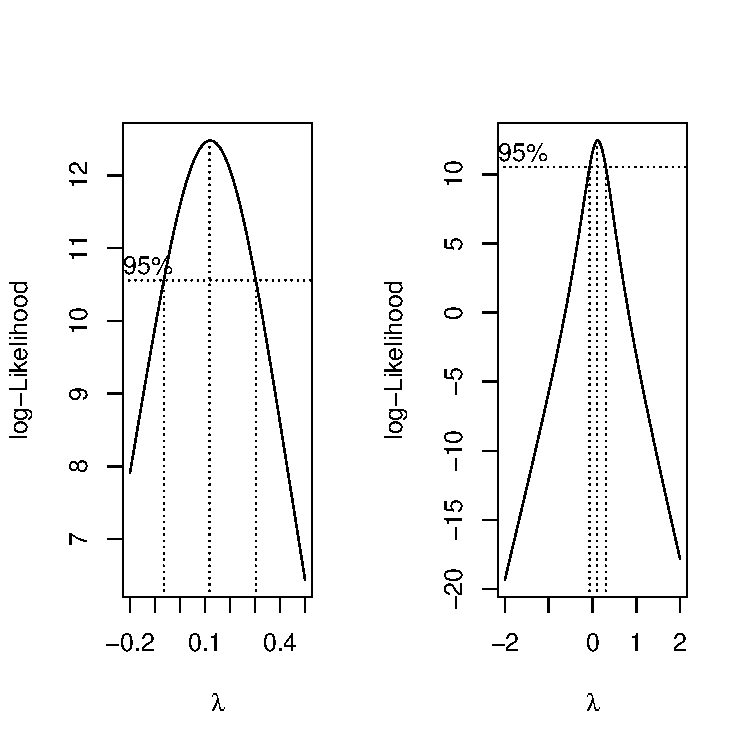
\includegraphics[width=.45\linewidth]{figure/fig-unnamed-chunk-34-1}

}



\end{knitrout}
\end{center}
\caption{Residuals versus the Fitted Values for Simple Linear Model in Problem 5 b)} \label{fig:simple:bact3}
\end{figure}

Figure~\ref{fig:simple:bact3} shows a plot of the studentized residuals versus the fitted values. The plot suggests a clear curve, which is usually an indicator of non-linearity. This is in line with the previous comments.

Finally, this model is inadequate and transformations on the response variables are required.

\item The Box-Cox method is used to determine which transformation is optimal. Figure~\ref{fig:simple:bact4} shows the plot of the log-likelihood function in terms of $\lambda$, for two different ranges of $\lambda$. It was obtained with the \textsf{R} commands:
\begin{knitrout}
\definecolor{shadecolor}{rgb}{0.969, 0.969, 0.969}\color{fgcolor}\begin{kframe}
\begin{alltt}
\hlkwd{boxCox}\hlstd{(bact}\hlopt{~}\hlstd{min,} \hlkwc{lambda} \hlstd{=} \hlkwd{seq}\hlstd{(}\hlopt{-}\hlnum{2}\hlstd{,} \hlnum{2}\hlstd{,} \hlkwc{len} \hlstd{=} \hlnum{20}\hlstd{),} \hlkwc{plotit} \hlstd{=} \hlnum{TRUE}\hlstd{)}
\hlkwd{boxCox}\hlstd{(bact}\hlopt{~}\hlstd{min,} \hlkwc{lambda} \hlstd{=} \hlkwd{seq}\hlstd{(}\hlopt{-}\hlnum{0.2}\hlstd{,} \hlnum{0.5}\hlstd{,} \hlkwc{len} \hlstd{=} \hlnum{20}\hlstd{),} \hlkwc{plotit} \hlstd{=} \hlnum{TRUE}\hlstd{)}
\end{alltt}
\end{kframe}
\end{knitrout}

\begin{figure}
\begin{center}
\begin{knitrout}
\definecolor{shadecolor}{rgb}{0.969, 0.969, 0.969}\color{fgcolor}

{\centering 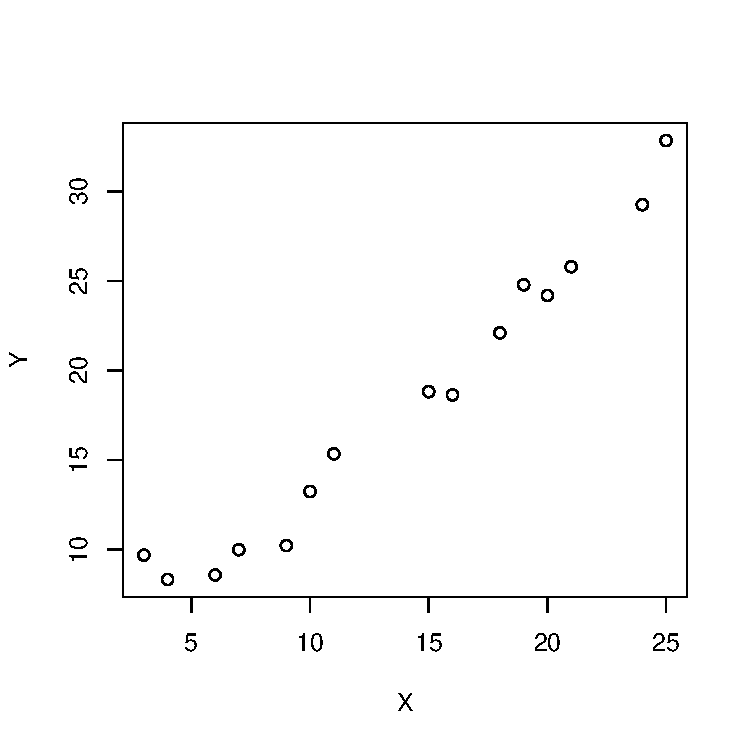
\includegraphics[width=.45\linewidth]{figure/fig-unnamed-chunk-36-1}

}



\end{knitrout}
\end{center}
\caption{Log-likelihood versus $\lambda$ in the Box-Cox method for Problem 5 c)} \label{fig:simple:bact4}
\end{figure}

Note that the maximum is around 0.1 and 0 is included in the 95\% confidence interval for $\lambda$. Therefore, it is preferable to use 0 as this is a common transformation, it represents the logarithm transformation. Let $y^{*}=\ln(y)$. A simple linear model is fitted to the transformed data. The output is the following:
\begin{knitrout}
\definecolor{shadecolor}{rgb}{0.969, 0.969, 0.969}\color{fgcolor}\begin{kframe}
\begin{alltt}
\hlstd{logbact} \hlkwb{<-} \hlkwd{log}\hlstd{(bact)}
\hlstd{fit2} \hlkwb{<-} \hlkwd{lm}\hlstd{(logbact}\hlopt{~}\hlstd{min)}
\hlkwd{summary}\hlstd{(fit2)}
\end{alltt}
\begin{verbatim}
##
## Call:
## lm(formula = logbact ~ min)
##
## Residuals:
##       Min        1Q    Median        3Q       Max
## -0.184303 -0.083994  0.001453  0.072825  0.206246
##
## Coefficients:
##             Estimate Std. Error t value Pr(>|t|)
## (Intercept)  5.33878    0.07409   72.05 6.47e-15 ***
## min         -0.23617    0.01007  -23.46 4.49e-10 ***
## ---
## Signif. codes:
## 0 '***' 0.001 '**' 0.01 '*' 0.05 '.' 0.1 ' ' 1
##
## Residual standard error: 0.1204 on 10 degrees of freedom
## Multiple R-squared:  0.9822,	Adjusted R-squared:  0.9804
## F-statistic: 550.3 on 1 and 10 DF,  p-value: 4.489e-10
\end{verbatim}
\end{kframe}
\end{knitrout}

The fitted model is $$\hat{y}^{*}=5.33878-0.23617x,$$ where the parameters of the model are estimated by the best linear unbiased estimators. Figure~\ref{fig:simple:bact5} is a scatter plot of the transformed response variable versus the covariate, along with the fitted line. The scatter plot looks much more linear now than in (a).

\begin{figure}
\begin{center}
\begin{knitrout}
\definecolor{shadecolor}{rgb}{0.969, 0.969, 0.969}\color{fgcolor}

{\centering 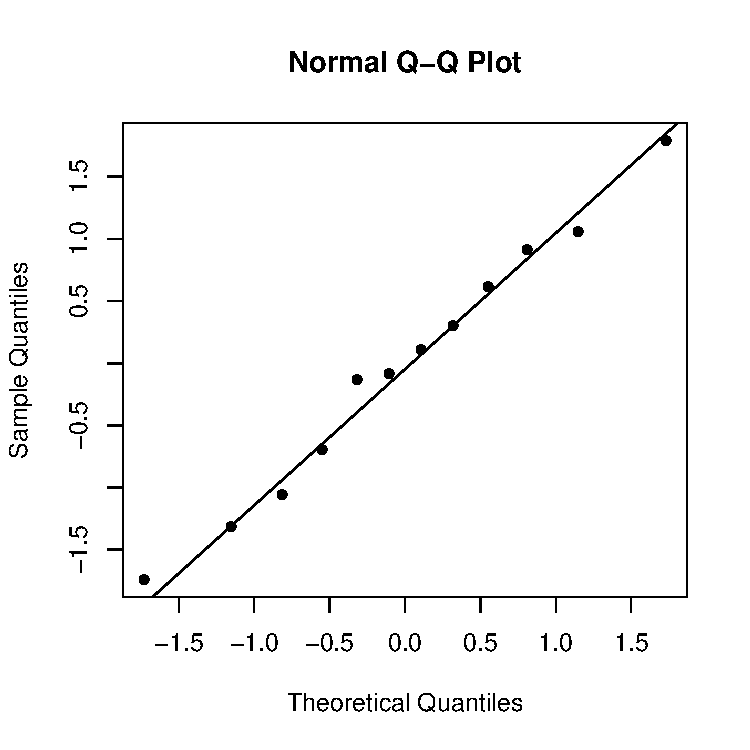
\includegraphics[width=.45\linewidth]{figure/fig-unnamed-chunk-38-1}

}



\end{knitrout}
\end{center}
\caption{Scatter Plot of the Logarithm of the Number of Bacteria versus the Minutes of Exposure to $300^{o}$ F}
\label{fig:simple:bact5}
\end{figure}

The ANOVA table is obtained using \textsf{R}:
\begin{knitrout}
\definecolor{shadecolor}{rgb}{0.969, 0.969, 0.969}\color{fgcolor}\begin{kframe}
\begin{alltt}
\hlkwd{anova}\hlstd{(fit2)}
\end{alltt}
\begin{verbatim}
## Analysis of Variance Table
##
## Response: logbact
##           Df Sum Sq Mean Sq F value    Pr(>F)
## min        1 7.9761  7.9761  550.33 4.489e-10 ***
## Residuals 10 0.1449  0.0145
## ---
## Signif. codes:
## 0 '***' 0.001 '**' 0.01 '*' 0.05 '.' 0.1 ' ' 1
\end{verbatim}
\end{kframe}
\end{knitrout}

The F-statistic for the test of significance of regression is 550.33, and it has 1 and 10 degrees of freedom, so the $p$-value is $$P[F_{(1,10)}>550.33]= 4.489\times10^{-10}.$$ Since the $p$-value is much smaller than 1\%, there is enough evidence to reject the null hypothesis that $\beta_{1}=0$ at the 1\% level. This model is significant.

The value of $R^{2}$ is very high at $98.22\%$. This means that about 98\% of the variation in the log of the number of bacteria in the canned food is explained by the minutes of exposure to $300^{o}$F. The model seems to perform very well, better than the model proposed in (b).

The Q-Q Plot of the studentized residuals is shown in Figure~\ref{fig:simple:bact6}. The dots are beautifully aligned with the standard normal quantiles. The normality assumption is appropriate. Figure~\ref{fig:simple:bact7} shows a plot of the studentized residuals versus the fitted values. The dots can be contained in horizontal bands and looks randomly scattered.

Finally, this model is adequate and the transformation used on the response variables fixed the problems in the model.

\begin{figure}
\begin{center}
\begin{knitrout}
\definecolor{shadecolor}{rgb}{0.969, 0.969, 0.969}\color{fgcolor}

{\centering \includegraphics[width=.45\linewidth]{figure/fig-unnamed-chunk-40-1}

}



\end{knitrout}
\end{center}
\caption{Q-Q Plot of Model for the Logarithm of the Number of Bacteria in Problem 5 c)} \label{fig:simple:bact6}
\end{figure}

\begin{figure}
\begin{center}
\begin{knitrout}
\definecolor{shadecolor}{rgb}{0.969, 0.969, 0.969}\color{fgcolor}

{\centering 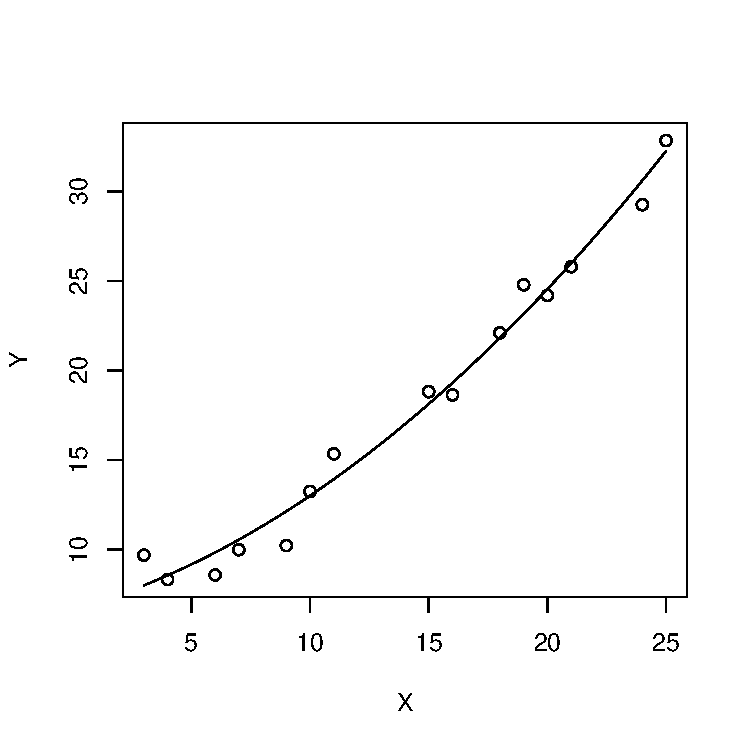
\includegraphics[width=.45\linewidth]{figure/fig-unnamed-chunk-41-1}

}



\end{knitrout}
\end{center}
\caption{Residuals versus the Fitted Values for Model for the Logarithm of the Number of Bacteria in Problem 5 c)}
\label{fig:simple:bact7}
\end{figure}

\end{enumerate}
\end{solution}

\newpage
\section*{Chapitre \ref{chap:multiple}}
\addcontentsline{toc}{section}{Chapitre \protect\ref{chap:multiple}}

\begin{solution}{3.1}
    Tout d'abord, selon le théorème
    \ref{thm:elements:derivee_fonction} de l'annexe
    \ref{chap:elements},
    \begin{displaymath}
      \frac{d}{d \mat{x}}\, f(\mat{x})^\prime \mat{A} f(\mat{x}) =
      2 \left( \frac{d}{d \mat{x}} f(\mat{x}) \right)^\prime \mat{A} f(\mat{x}).
    \end{displaymath}
    Il suffit, pour faire la démonstration, d'appliquer directement ce
    résultat à la forme quadratique
    \begin{displaymath}
      S(\betavec) = (\mat{y} - \mat{X} \betavec)^\prime (\mat{y} - \mat{X} \betavec)
    \end{displaymath}
    avec $f(\betavec) = \mat{y} - \mat{X} \betavec$ et $\mat{A} =
    \mat{I}$, la matrice identité. On a alors
    \begin{align*}
      \frac{d}{d\betavec} S(\betavec)
      &= 2
      \left(
        \frac{d}{d\betavec} (\mat{y} - \mat{X} \betavec)
      \right)^\prime
      \mat{y} - \mat{X} \betavec \\
      &= 2 (-\mat{X})^\prime (\mat{y} - \mat{X} \betavec)\\
      &= -2 \mat{X}^\prime (\mat{y} - \mat{X} \betavec).
    \end{align*}
    En posant ces dérivées exprimées sous forme matricielle
    simultanément égales à zéro, on obtient les équations normales à
    résoudre pour calculer l'estimateur des moindres carrés du vecteur
    $\betavec$, soit
    \begin{displaymath}
      \mat{X}^\prime \mat{X} \hat\betavec = \mat{X}^\prime \mat{y}.
    \end{displaymath}
    En isolant $\hat\betavec$ dans l'équation ci-dessus, on obtient,
    finalement, l'estimateur des moindres carrés:
    \begin{displaymath}
      \hat\betavec = (\mat{X}^\prime \mat{X})^{-1} \mat{X}^\prime \mat{y}.
    \end{displaymath}
  
\end{solution}
\begin{solution}{3.2}
    \begin{enumerate}
    \item On a un modèle sans variable explicative. Intuitivement, la
      meilleure prévision de $Y_t$ sera alors $\bar{Y}$. En effet,
      pour ce modèle,
      \begin{displaymath}
        \mat{X} =
        \begin{bmatrix}
          1 \\ \vdots \\ 1
        \end{bmatrix}_{n \times 1}
      \end{displaymath}
      et
      \begin{align*}
        \hat\betavec
        &=\left(\mat{X}^\prime \mat{X} \right)^{-1} \mat{X}^\prime
        \mat{y} \\
        &=
        \left(
          \begin{bmatrix}
            1 & \cdots & 1
          \end{bmatrix}
          \begin{bmatrix}
            1 \\ \vdots \\ 1
          \end{bmatrix}
        \right)^{-1}
        \begin{bmatrix}
          1 & \cdots & 1
        \end{bmatrix}
        \begin{bmatrix}
          Y_1 \\ \vdots \\ Y_n
        \end{bmatrix}\\
        &= n^{-1} \sum_{t=1}^n Y_t \\
        &= \bar{Y}.
      \end{align*}
    \item Il s'agit du modèle de régression linéaire simple passant
      par l'origine, pour lequel la matrice de schéma est
      \begin{displaymath}
        \mat{X} =
        \begin{bmatrix}
          X_1 \\ \vdots \\ X_n
        \end{bmatrix}_{n \times 1}.
      \end{displaymath}
      Par conséquent,
      \begin{align*}
        \hat\betavec
        &=
        \left(
          \begin{bmatrix}
            X_1 & \cdots & X_n
          \end{bmatrix}
          \begin{bmatrix}
            X_1 \\ \vdots \\ X_n
          \end{bmatrix}
        \right)^{-1}
        \begin{bmatrix}
          X_1 & \cdots & X_n
        \end{bmatrix}
        \begin{bmatrix}
          Y_1 \\ \vdots \\ Y_n
        \end{bmatrix} \\
        &=
        \left(
          \sum_{t=1}^n X_t^2
        \right)^{-1} \sum_{t=1}^n X_tY_t \\
        &= \frac{\sum_{t=1}^n X_t Y_t}{\sum_{t=1}^n X_t^2},
      \end{align*}
      tel qu'obtenu à l'exercice
      \ref{chap:simple}.\ref{ex:simple:origine}.
    \item On est ici en présence d'un modèle de régression multiple ne
      passant pas par l'origine et ayant deux variables explicatives.
      La matrice de schéma est alors
      \begin{displaymath}
        \mat{X} =
        \begin{bmatrix}
          1      & X_{11}  & X_{12} \\
          \vdots & \vdots & \vdots \\
          1      & X_{n1}  & X_{n2}
        \end{bmatrix}_{n \times 3}.
      \end{displaymath}
      Par conséquent,
      \begin{align*}
        \hat\betavec
        &=
        \left(
          \begin{bmatrix}
            1     & \cdots & 1      \\
            X_{11} & \cdots & X_{n1} \\
            X_{12} & \cdots & X_{n2}
          \end{bmatrix}
          \begin{bmatrix}
            1      & X_{11}  & X_{12} \\
            \vdots & \vdots & \vdots \\
            1      & X_{n1}  & X_{n2}
          \end{bmatrix}
        \right)^{-1}
        \begin{bmatrix}
          1     & \cdots & 1      \\
          X_{11} & \cdots & X_{n1} \\
          X_{12} & \cdots & X_{n2}
        \end{bmatrix}
        \begin{bmatrix}
          Y_1 \\ \vdots \\ Y_n
        \end{bmatrix} \\
        & =
        \begin{bmatrix}
          n           & n \bar{X}_1             & n \bar{X}_2 \\
          n \bar{X}_1 & \sum_{t=1}^n X_{t1}^2    & \sum_{t=1}^n X_{t1}X_{t2} \\
          n \bar{X}_2 & \sum_{t=1}^n X_{t1}X_{t2} & \sum_{t=1}^n X_{t2}^2
        \end{bmatrix}^{-1}
        \begin{bmatrix}
          \sum_{t=1}^n Y_t \\ \sum_{t=1}^n X_{t1}Y_t \\ \sum_{t=1}^n
          X_{t2}Y_t
        \end{bmatrix}.
      \end{align*}
      L'inversion de la première matrice et le produit par la seconde
      sont laissés aux bons soins du lecteur plus patient que les
      rédacteurs de ces solutions.
    \end{enumerate}
  
\end{solution}
\begin{solution}{3.3}
    Dans le modèle de régression linéaire simple, la matrice schéma est
    \begin{displaymath}
      \mat{X} =
      \begin{bmatrix}
        1      & X_1    \\
        \vdots & \vdots \\
        1      & X_n
      \end{bmatrix}.
    \end{displaymath}
    Par conséquent,
    \begin{align*}
      \var{\hat\betavec}
      &= \sigma^2 (\mat{X}^\prime \mat{X})^{-1} \\
      &= \sigma^2
      \left(
        \begin{bmatrix}
          1   & \cdots & 1  \\
          X_1 & \cdots & X_n
        \end{bmatrix}
        \begin{bmatrix}
          1      & X_1    \\
          \vdots & \vdots \\
          1      & X_n
        \end{bmatrix}
      \right)^{-1} \\
      &= \sigma^2
      \begin{bmatrix}
        n         & n \bar{X}        \\
        n \bar{X} & \sum_{t=1}^n X_t^2
      \end{bmatrix}^{-1}\\
      &= \frac{\sigma^2}{n \sum_{t=1}^n X_t^2 - n^2 \bar{X}^2}
      \begin{bmatrix}
        \sum_{t=1}^n X_t^2 & -n \bar{X} \\
        -n \bar{X}        & n
      \end{bmatrix} \\
      &= \frac{\sigma^2}{\sum_{t=1}^n (X_t - \bar{X}^2)}
      \begin{bmatrix}
        n^{-1} \sum_{t=1}^n X_t^2 & -\bar{X} \\
        -\bar{X}                 & 1
      \end{bmatrix},
    \end{align*}
    d'où
    \begin{align*}
      \var{\hat{\beta}_0}
      &= \sigma^2\, \frac{\sum_{t=1}^n X_t^2}{%
        n \sum_{t=1}^n (X_t - \bar{X})^2} \\
      &= \sigma^2\, \frac{\sum_{t=1}^n (X_t - \bar{X}^2) + n \bar{X}^2}{%
        n \sum_{t=1}^n (X_t - \bar{X})^2} \\
      \intertext{et}
      \var{\hat{\beta}_1}
      &= \frac{\sigma^2}{\sum_{t=1}^n (X_t - \bar{X})^2}.
    \end{align*}
    Ceci correspond aux résultats antérieurs.
  
\end{solution}
\begin{solution}{3.4}
    Dans les démonstrations qui suivent, trois relations de base
    seront utilisées:
    $\mat{e} = \mat{y - \hat{y}}$,
    $\mat{\hat{y}} = \mat{X} \hat\betavec$ et
    $\hat\betavec = (\mat{X}^\prime \mat{X})^{-1} \mat{X}^\prime \mat{y}$.
    \begin{enumerate}
    \item On a
      \begin{align*}
        \mat{X}^\prime \mat{e}
        &= \mat{X}^\prime (\mat{y - \hat{y}}) \\
        &= \mat{X}^\prime (\mat{y} - \mat{X} \hat\betavec) \\
        &= \mat{X}^\prime \mat{y} - (\mat{X}^\prime \mat{X}) \hat\betavec \\
        &= \mat{X}^\prime \mat{y} - (\mat{X}^\prime \mat{X})
        (\mat{X}^\prime \mat{X})^{-1} \mat{X}^\prime \mat{y} \\
        &= \mat{X}^\prime \mat{y} - \mat{X}^\prime \mat{y} \\
        &= \mat{0}.
      \end{align*}
      En régression linéaire simple, cela donne
      \begin{align*}
        \mat{X}^\prime \mat{e} &=
        \begin{bmatrix}
          1   & \cdots & 1  \\
          X_1 & \cdots & X_n
        \end{bmatrix}
        \begin{bmatrix}
          e_1 \\ \vdots \\ e_n
        \end{bmatrix} \\
        &=
        \begin{bmatrix}
          \sum_{t=1}^n e_t \\
          \sum_{t=1}^n X_t e_t
        \end{bmatrix}.
      \end{align*}
      Par conséquent, $\mat{X}^\prime \mat{e} = \mat{0}$ se simplifie
      en $\sum_{t=1}^n e_t = 0$ et $\sum_{t=1}^n X_t e_t = 0$ soit,
      respectivement, la condition pour que l'estimateur des moindres
      carrés soit sans biais et la seconde équation normale obtenue à
      la partie \ref{ex:simple:base:eq_normales}) de l'exercice
      \ref{chap:simple}.\ref{ex:simple:base}.
     \item On a
       \begin{align*}
         \hat{\mat{y}}^\prime \mat{e}
         &= (\mat{X}\hat\betavec)^\prime (\mat{y - \hat{y}}) \\
         &= \hat\betavec^\prime \mat{X}^\prime (\mat{y} - \mat{X}\hat\betavec) \\
         &= \hat\betavec^\prime \mat{X}^\prime \mat{y} - \hat\betavec^\prime
         (\mat{X}^\prime \mat{X}) \hat\betavec \\
         &= \hat\betavec^\prime \mat{X}^\prime \mat{y} - \hat\betavec^\prime
         (\mat{X}^\prime \mat{X}) (\mat{X}^\prime \mat{X})^{-1}
         \mat{X}^\prime \mat{y} \\
         &= \hat\betavec^\prime \mat{X}^\prime \mat{y} - \hat\betavec^\prime
         \mat{X}^\prime \mat{y} \\
         &= 0.
       \end{align*}
       Pour tout modèle de régression cette équation peut aussi
       s'écrire sous la forme plus conventionnelle $\sum_{t=1}^n
       \hat{Y}_t e_t = 0$. Cela signifie que le produit scalaire entre
       le vecteur des prévisions et celui des erreurs doit être nul
       ou, autrement dit, que les vecteurs doivent être orthogonaux.
       C'est là une condition essentielle pour que l'erreur
       quadratique moyenne entre les vecteurs $\mat{y}$ et
       $\mat{\hat{y}}$ soit minimale. (Pour de plus amples détails sur
       l'interprétation géométrique du modèle de régression, consulter
       {\shorthandoff{:} \citet[chapitres 20 et
         21]{Draper:regression:1998}}.)
         D'ailleurs, on constate que
       $\hat{\mat{y}}^\prime \mat{e} = \hat\betavec^\prime \mat{X}^\prime
       \mat{e}$ et donc, en supposant sans perte de généralité que
       $\hat\betavec \ne \mat{0}$,
       que $\hat{\mat{y}}^\prime \mat{e} = 0$
       et $\mat{X}^\prime \mat{e} = \mat{0}$ sont des conditions en
       tous points équivalentes.
     \item On a
       \begin{align*}
         \mat{\hat{y}}^\prime \mat{\hat{y}}
         &= (\mat{X} \hat\betavec)^\prime \mat{X} \hat\betavec \\
         &= \hat\betavec^\prime (\mat{X}^\prime \mat{X}) \hat\betavec \\
         &= \hat\betavec^\prime (\mat{X}^\prime \mat{X}) (\mat{X}^\prime
         \mat{X})^{-1} \mat{X}^\prime \mat{y} \\
         &= \hat\betavec^\prime \mat{X}^\prime \mat{y}.
       \end{align*}
       Cette équation est l'équivalent matriciel de l'identité
       \begin{align*}
         \SSR
         &= \hat{\beta}_1^2 \sum_{t = 1}^n (X_t - \bar{X})^2 \\
         &= \frac{S_{XY}^2}{S_{XX}}
       \end{align*}
       utilisée à plusieurs reprises dans les solutions du chapitre
       \ref{chap:simple}.  En effet, en régression linéaire simple,
       $\mat{\hat{y}}^\prime \mat{\hat{y}} = \sum_{t = 1}^n
       \hat{Y}_t^2 = \sum_{t = 1}^n (\hat{Y} - \bar{Y})^2 + n
       \bar{Y}^2 = \SSR + n \bar{Y}^2$ et
       \begin{align*}
         \hat\betavec^\prime \mat{X}^\prime \mat{y}
         &= \hat{\beta}_0 n \bar{Y} + \hat{\beta}_1 \sum_{t = 1}^n X_t Y_t \\
         &= (\bar{Y} - \hat{\beta}_1 \bar{X}) n \bar{Y} +
         \hat{\beta}_1 \sum_{t = 1}^n X_t Y_t \\
         &= \hat{\beta}_1 \sum_{t = 1}^n (X_t - \bar{X})(Y_t -
         \bar{Y}) + n \bar{Y}^2 \\
         &= \frac{S_{XY}^2}{S_{XX}} + n \bar{Y}^2,
       \end{align*}
       d'où $\SSR = S_{XY}^2/S_{XX}$.
     \end{enumerate}
   
\end{solution}
\begin{solution}{3.5}
    \begin{enumerate}
    \item Premièrement, $Y_0 = \mat{x}_0 \betavec + \varepsilon_0$ avec
      $\esp{\varepsilon_0} = 0$. Par conséquent, $\esp{Y_0} = \esp{x_0
        \betavec + \varepsilon_0} = \mat{x}_0 \betavec$. Deuxièmement,
      $\esp{\hat{Y}_0} = \esp{\mat{x}_0 \hat\betavec} = \mat{x}_0
      \esp{\hat\betavec} = x_0 \betavec$ puisque l'estimateur des moindres
      carrés de $\betavec$ est sans biais. Ceci complète la preuve.
    \item Tout d'abord, $\esp{(\hat{Y}_0 - \esp{Y_0})^2} =
      \varmat{\hat{Y}_0} = \var{\hat{Y}_0}$ puisque la matrice de
      variance-covariance du vecteur aléatoire $\hat{Y}_0$ ne
      contient, ici, qu'une seule valeur. Or, par le théorème
      \ref{thm:elements:esp_var},
       \begin{align*}
         \var{\hat{Y}_0}
         &= \varmat{\mat{x}_0 \hat\betavec} \\
         &= \mat{x}_0 \varmat{\hat\betavec} \mat{x}_0^\prime \\
         &= \sigma^2 \mat{x}_0 (\mat{X}^\prime \mat{X})^{-1}
         \mat{x}_0^\prime.
       \end{align*}
       Afin de construire un intervalle de confiance pour $\esp{Y_0}$,
       on ajoute au modèle l'hypothèse $\epsvec \sim N(\mat{0}, \sigma^2
       \mat{I})$. Par linéarité de l'estimateur des moindres carrés,
       on a alors $\hat{Y}_0 \sim N(\esp{Y_0}, \var{\hat{Y}_0})$. Par
       conséquent,
       \begin{displaymath}
         \Pr
         \left[
           -z_{\alpha/2}
           \leq
           \frac{\hat{Y} - \esp{\hat{Y}_0}}{\sqrt{\var{\hat{Y}_0}}}
           \leq
           z_{\alpha/2}
         \right] = 1 - \alpha
       \end{displaymath}
       d'où un intervalle de confiance de niveau $1 - \alpha$ pour
       $\esp{Y_0}$ est
       \begin{displaymath}
         \esp{Y_0}
         \in \hat{Y}_0 \pm z_{\alpha/2}\, \sigma\,
         \sqrt{\mat{x}_0 (\mat{X}^\prime \mat{X})^{-1} \mat{x}_0^\prime}.
       \end{displaymath}
       Si la variance $\sigma^2$ est inconnue et estimée par $s^2$,
       alors la distribution normale est remplacée par une
       distribution de Student avec $n - p - 1$ degrés de
       liberté. L'intervalle de confiance devient alors
       \begin{displaymath}
         \esp{Y_0}
         \in \hat{Y}_0 \pm t_{\alpha/2}(n - p - 1)\, s\,
         \sqrt{\mat{x}_0 (\mat{X}^\prime \mat{X})^{-1} \mat{x}_0^\prime}.
       \end{displaymath}
     \item Par le résultat obtenu en a) et en supposant que
       $\Cov(\varepsilon_0, \varepsilon_t) = 0$ pour tout $t = 1,
       \dots, n$, on a
       \begin{align*}
         \esp{(Y_0 - \hat{Y}_0)^2}
         &= \var{Y_0 - \hat{Y}_0} \\
         &= \var{Y_0} + \var{\hat{Y}_0} \\
         &= \sigma^2 (1 + \mat{x}_0 (\mat{X}^\prime \mat{X})^{-1}
         \mat{x}_0^\prime).
       \end{align*}
       Ainsi, avec l'hypothèse sur le terme d'erreur énoncée en b),
       $Y_0 - \hat{Y}_0 \sim N(0, \var{Y_0 - \hat{Y}_0})$. En suivant
       le même cheminement qu'en b), on détermine qu'un intervalle de
       confiance de niveau $1 - \alpha$ pour $Y_0$ est
       \begin{displaymath}
         Y_0
         \in \hat{Y}_0 \pm z_{\alpha/2}\, \sigma\,
         \sqrt{1 + \mat{x}_0 (\mat{X}^\prime \mat{X})^{-1} \mat{x}_0^\prime}.
       \end{displaymath}
       ou, si la variance $\sigma^2$ est inconnue et estimée par
       $s^2$,
       \begin{displaymath}
         Y_0
         \in \hat{Y}_0 \pm t_{\alpha/2}(n - p - 1)\, s\,
         \sqrt{1 + \mat{x}_0 (\mat{X}^\prime \mat{X})^{-1} \mat{x}_0^\prime}.
       \end{displaymath}
     \end{enumerate}
   
\end{solution}
\begin{solution}{3.6}
    On a la relation suivante liant la statistique $F$ et le
    coefficient de détermination $R^2$:
    \begin{displaymath}
      F = \frac{R^2}{1 - R^2}\, \frac{n - p - 1}{p}
    \end{displaymath}
    La principale inconnue dans le problème est $n$, le nombre de
    données. Or,
    \begin{align*}
      n
      &= p F \left( \frac{1 - R^2}{R^2} \right) + p + 1 \\
      &= 3 (5,438) \left( \frac{1 - 0,521}{0,521} \right) + 3 + 1 \\
      &= 19.
    \end{align*}
    Soit $F$ une variable aléatoire dont la distribution est une loi
    de Fisher avec $3$ et $19 - 3 - 1 = 15$ degrés de liberté, soit la
    même distribution que la statistique $F$ du modèle. On obtient la
    valeur $p$ du test global de validité du modèle dans un tableau de
    quantiles de la distribution $F$ ou avec la fonction \texttt{pf}
    dans R:
    \begin{align*}
      \Pr[F > 5,438] = 0,0099
    \end{align*}
  
\end{solution}
\begin{solution}{3.7}
    \begin{enumerate}
    \item On a
      \begin{align*}
        \hat\betavec
        &= (\mat{X}^\prime \mat{X})^{-1} \mat{X}^\prime \mat{y} \\
        &= \frac{1}{2}
        \left[
          \begin{array}{rrrr}
            -6 & 34 & -13 & -13 \\
            2 & -4 &   1 &   1 \\
            0 & -2 & 1 & 1
          \end{array}
        \right]
        \begin{bmatrix}
          17 \\ 12 \\ 14 \\ 13
        \end{bmatrix} \\
        &= \frac{1}{2}
        \left[
          \begin{array}{r}
            -45 \\ 13 \\ 3
          \end{array}
        \right] =
        \left[
          \begin{array}{r}
            -22,5 \\ 6,5 \\ 1,5
          \end{array}
        \right]
      \end{align*}
    \item Avec les résultats de la partie a), on a
      \begin{align*}
        \mat{\hat{y}} &= \mat{X} \hat\betavec =
        \begin{bmatrix}
          17 \\ 12 \\ 13,5 \\ 13,5
        \end{bmatrix}, \\
        \mat{e} &= \mat{y} - \mat{\hat{y}} =
        \left[
          \begin{array}{r}
            0 \\ 0 \\ 0,5 \\ -0,5
          \end{array}
        \right]
      \end{align*}
      et $\bar{Y} = 14$. Par conséquent,
      \begin{align*}
        \SST
        &= \mat{y}^\prime \mat{y} - n \bar{Y}^2 = 14 \\
        \SSE
        &= \mat{e}^\prime \mat{e} = 0,5 \\
        \SSR &= \SST - \SSR = 13,5,
      \end{align*}
      d'où le tableau d'analyse de variance est le suivant:
      \begin{center}
        \begin{tabular}{lrrrr}
          \toprule
          Source & SS & d.l. & MS & $F$ \\
          \midrule
          Régression & $13,5$ & 2 & $6,75$ &  $13,5$ \\
          Erreur     &  $0,5$ & 1 &  $0,5$ \\
          \midrule
          Total      &   $14$ & \\
          \bottomrule
        \end{tabular}
      \end{center}
      Le coefficient de détermination est
      \begin{displaymath}
        R^2 = 1 - \frac{\SSE}{\SST} = 0,9643.
      \end{displaymath}
    \item On sait que $\var{\hat{\beta}_i} = \sigma^2 c_{ii}$, où
      $c_{ii}$ est l'élément en position $(i+1, i+1)$ de la matrice
      $(\mat{X}^\prime \mat{X})^{-1}$. Or, $\hat{\sigma}^2 = s^2 =
      \text{MSE} = 0,5$, tel que calculé en b). Par conséquent, la
      statistique $t$ du test $H_0: \beta_1 = 0$ est
      \begin{displaymath}
        t
        = \frac{\hat{\beta}_1}{s \sqrt{c_{11}}}
        = \frac{6,5}{\sqrt{0,5 (\frac{11}{2})}}
        = 3,920,
      \end{displaymath}
      alors que celle du test $H_0: \beta_2 = 0$ est
      \begin{displaymath}
        t
        = \frac{\hat{\beta}_2}{s \sqrt{c_{22}}}
        = \frac{1,5}{\sqrt{0,5 (\frac{3}{2})}}
        = 1,732.
      \end{displaymath}
      À un niveau de signification de 5~\%, la valeur critique de ces
      tests est $t_{0,025}(1) = 12,706$. Dans les deux cas, on ne
      rejette donc pas $H_0$, les variables $X_1$ et $X_2$ ne sont pas
      significatives dans le modèle.
    \item Soit $\mat{x}_0 = \begin{bmatrix} 1 & 3,5 & 9 \end{bmatrix}$
      et $Y_0$ la valeur de la variable dépendante correspondant à
      $\mat{x}_0$. La prévision de $Y_0$ donnée par le modèle trouvé
      en a) est
      \begin{align*}
        \hat{Y}_0
        &= \mat{x}_0 \hat\betavec \\
        &= -22,5 + 6,5(3,5) + 1,5(9) \\
        &= 13,75.
      \end{align*}
      D'autre part,
      \begin{align*}
        \widehat{\text{Var}}[Y_0 - \hat{Y}_0]
        &= s^2 (1 + \mat{x}_0 (\mat{X}^\prime \mat{X})^{-1} \mat{x}_0^\prime) \\
        &= 1,1875.
      \end{align*}
      Par conséquent, un intervalle de confiance à 95~\% pour $Y_0$
      est
      \begin{align*}
        \esp{Y_0} &\in \hat{Y}_0 \pm t_{0,025}(1) s \sqrt{1 + \mat{x}_0
          (\mat{X}^\prime \mat{X})^{-1} \mat{x}_0^\prime} \\
        &\in 13,75 \pm 12,706 \sqrt{1,1875} \\
        &\in (-0,096, 27,596).
      \end{align*}
    \end{enumerate}
  
\end{solution}
\begin{solution}{3.8}
    \begin{enumerate}
    \item On importe les données dans \textsf{R}, puis on effectue les
      conversions nécessaires. Comme précédemment, la variable
      \texttt{consommation} contient la consommation des voitures en
      $\ell$/100~km et la variable \texttt{poids} le poids en
      kilogrammes. On ajoute la variable \texttt{cylindree}, qui
      contient la cylindrée des voitures en litres.
\begin{knitrout}
\definecolor{shadecolor}{rgb}{0.969, 0.969, 0.969}\color{fgcolor}\begin{kframe}
\begin{alltt}
\hlstd{carburant} \hlkwb{<-} \hlkwd{read.table}\hlstd{(}\hlstr{"carburant.dat"}\hlstd{,} \hlkwc{header} \hlstd{=} \hlnum{TRUE}\hlstd{)}
\hlstd{consommation} \hlkwb{<-} \hlnum{235.1954}\hlopt{/}\hlstd{carburant}\hlopt{$}\hlstd{mpg}
\hlstd{poids} \hlkwb{<-} \hlstd{carburant}\hlopt{$}\hlstd{poids} \hlopt{*} \hlnum{0.45455} \hlopt{*} \hlnum{1000}
\hlstd{cylindree} \hlkwb{<-} \hlstd{carburant}\hlopt{$}\hlstd{cylindree} \hlopt{*} \hlnum{2.54}\hlopt{^}\hlnum{3}\hlopt{/}\hlnum{1000}
\end{alltt}
\end{kframe}
\end{knitrout}
    \item La fonction \texttt{summary} fournit l'information
      essentielle pour juger de la validité et de la qualité du
      modèle:
\begin{knitrout}
\definecolor{shadecolor}{rgb}{0.969, 0.969, 0.969}\color{fgcolor}\begin{kframe}
\begin{alltt}
\hlstd{fit} \hlkwb{<-} \hlkwd{lm}\hlstd{(consommation} \hlopt{~} \hlstd{poids} \hlopt{+} \hlstd{cylindree)}
\hlkwd{summary}\hlstd{(fit)}
\end{alltt}
\begin{verbatim}
##
## Call:
## lm(formula = consommation ~ poids + cylindree)
##
## Residuals:
##     Min      1Q  Median      3Q     Max
## -1.8799 -0.5595  0.1577  0.6051  1.7900
##
## Coefficients:
##              Estimate Std. Error t value Pr(>|t|)
## (Intercept) -3.049304   1.098281  -2.776  0.00877 **
## poids        0.012677   0.001512   8.386 6.85e-10 ***
## cylindree   -1.122696   0.333479  -3.367  0.00186 **
## ---
## Signif. codes:
## 0 '***' 0.001 '**' 0.01 '*' 0.05 '.' 0.1 ' ' 1
##
## Residual standard error: 0.9156 on 35 degrees of freedom
## Multiple R-squared:  0.8927,	Adjusted R-squared:  0.8866
## F-statistic: 145.6 on 2 and 35 DF,  p-value: < 2.2e-16
\end{verbatim}
\end{kframe}
\end{knitrout}
      Le modèle est donc le suivant:
      \begin{displaymath}
        Y_t =
        -3,049 +
        0,01268 X_{t1} +
        -1,123 X_{t2} +
        \varepsilon_t,
        \quad
        \epsvec_t \sim N(0,
        0,9156^2 \mat{I})
      \end{displaymath}
      où $Y_t$ est la consommation en litres aux 100 kilomètres,
      $X_{t1}$ le poids en kilogrammes et $X_{t2}$ la cylindrée en
      litres. La faible valeur $p$ du test $F$ indique une régression
      globalement très significative. Les tests $t$ des paramètres
      individuels indiquent également que les deux variables du modèle
      sont significatives. Enfin, le $R^2$ de %
      0,8927 %$
      confirme que l'ajustement du modèle est toujours bon.
    \item On veut calculer un intervalle de confiance pour la
      consommation prévue d'une voiture de \nombre{1350}~kg ayant un
      moteur d'une cylindrée de 1,8 litres. On obtient, avec la
      fonction \texttt{predict}:
\begin{knitrout}
\definecolor{shadecolor}{rgb}{0.969, 0.969, 0.969}\color{fgcolor}\begin{kframe}
\begin{alltt}
\hlkwd{predict}\hlstd{(fit,} \hlkwc{newdata} \hlstd{=} \hlkwd{data.frame}\hlstd{(}\hlkwc{poids} \hlstd{=} \hlnum{1350}\hlstd{,} \hlkwc{cylindree} \hlstd{=} \hlnum{1.8}\hlstd{),}
        \hlkwc{interval} \hlstd{=} \hlstr{"prediction"}\hlstd{)}
\end{alltt}
\begin{verbatim}
##        fit      lwr      upr
## 1 12.04325 9.959855 14.12665
\end{verbatim}
\end{kframe}
\end{knitrout}
    \end{enumerate}
  
\end{solution}
\begin{solution}{3.9}
    Il y a plusieurs réponses possibles pour cet exercice. Si l'on
    cherche, tel que suggéré dans l'énoncé, à distinguer les voitures
    sport des minifourgonnettes (en supposant que ces dernières ont
    moins d'accidents que les premières), alors on pourrait
    s'intéresser, en premier lieu, à la variable \texttt{peak.rpm}. Il
    s'agit du régime moteur maximal, qui est en général beaucoup plus
    élevé sur les voitures sport. Puisque l'on souhaite expliquer le
    montant total des sinistres de différents types de voitures, il
    devient assez naturel de sélectionner également la variable
    \texttt{price}, soit le prix du véhicule. Un véhicule plus luxueux
    coûte en général plus cher à faire réparer à dommages égaux.
    Voyons l'effet de l'ajout, pas à pas, de ces deux variables au
    modèle précédent ne comportant que la variable
    \texttt{horsepower}:
\begin{knitrout}
\definecolor{shadecolor}{rgb}{0.969, 0.969, 0.969}\color{fgcolor}\begin{kframe}
\begin{alltt}
\hlstd{autoprice} \hlkwb{<-} \hlkwd{read.table}\hlstd{(}\hlstr{"data/auto-price.dat"}\hlstd{,} \hlkwc{header} \hlstd{=} \hlnum{TRUE}\hlstd{)}
\hlstd{fit1} \hlkwb{<-} \hlkwd{lm}\hlstd{(losses} \hlopt{~} \hlstd{horsepower} \hlopt{+} \hlstd{peak.rpm,} \hlkwc{data} \hlstd{= autoprice)}
\hlkwd{summary}\hlstd{(fit1)}
\end{alltt}
\begin{verbatim}
##
## Call:
## lm(formula = losses ~ horsepower + peak.rpm, data = autoprice)
##
## Residuals:
##     Min      1Q  Median      3Q     Max
## -67.973 -24.074  -6.373  18.049 130.301
##
## Coefficients:
##              Estimate Std. Error t value Pr(>|t|)
## (Intercept)  5.521414  29.967570   0.184 0.854060
## horsepower   0.318477   0.086840   3.667 0.000336 ***
## peak.rpm     0.016639   0.005727   2.905 0.004205 **
## ---
## Signif. codes:
## 0 '***' 0.001 '**' 0.01 '*' 0.05 '.' 0.1 ' ' 1
##
## Residual standard error: 33.44 on 156 degrees of freedom
## Multiple R-squared:  0.1314,	Adjusted R-squared:  0.1203
## F-statistic:  11.8 on 2 and 156 DF,  p-value: 1.692e-05
\end{verbatim}
\begin{alltt}
\hlkwd{anova}\hlstd{(fit1)}
\end{alltt}
\begin{verbatim}
## Analysis of Variance Table
##
## Response: losses
##             Df Sum Sq Mean Sq F value    Pr(>F)
## horsepower   1  16949 16948.5 15.1573 0.0001463 ***
## peak.rpm     1   9437  9437.0  8.4397 0.0042049 **
## Residuals  156 174435  1118.2
## ---
## Signif. codes:
## 0 '***' 0.001 '**' 0.01 '*' 0.05 '.' 0.1 ' ' 1
\end{verbatim}
\end{kframe}
\end{knitrout}
    La variable \texttt{peak.rpm} est significative, mais le $R^2$
    demeure faible. Ajoutons maintenant la variable \texttt{price} au modèle:
\begin{knitrout}
\definecolor{shadecolor}{rgb}{0.969, 0.969, 0.969}\color{fgcolor}\begin{kframe}
\begin{alltt}
\hlstd{fit2} \hlkwb{<-} \hlkwd{lm}\hlstd{(losses} \hlopt{~} \hlstd{horsepower} \hlopt{+} \hlstd{peak.rpm} \hlopt{+} \hlstd{price,} \hlkwc{data} \hlstd{= autoprice)}
\hlkwd{summary}\hlstd{(fit2)}
\end{alltt}
\begin{verbatim}
##
## Call:
## lm(formula = losses ~ horsepower + peak.rpm + price, data = autoprice)
##
## Residuals:
##     Min      1Q  Median      3Q     Max
## -66.745 -25.214  -5.867  18.407 130.032
##
## Coefficients:
##               Estimate Std. Error t value Pr(>|t|)
## (Intercept) -0.6972172 31.3221462  -0.022  0.98227
## horsepower   0.2414922  0.1408272   1.715  0.08838 .
## peak.rpm     0.0181386  0.0061292   2.959  0.00357 **
## price        0.0005179  0.0007451   0.695  0.48803
## ---
## Signif. codes:
## 0 '***' 0.001 '**' 0.01 '*' 0.05 '.' 0.1 ' ' 1
##
## Residual standard error: 33.49 on 155 degrees of freedom
## Multiple R-squared:  0.1341,	Adjusted R-squared:  0.1173
## F-statistic: 8.001 on 3 and 155 DF,  p-value: 5.42e-05
\end{verbatim}
\begin{alltt}
\hlkwd{anova}\hlstd{(fit2)}
\end{alltt}
\begin{verbatim}
## Analysis of Variance Table
##
## Response: losses
##             Df Sum Sq Mean Sq F value    Pr(>F)
## horsepower   1  16949 16948.5 15.1071 0.0001502 ***
## peak.rpm     1   9437  9437.0  8.4118 0.0042702 **
## price        1    542   542.1  0.4832 0.4880298
## Residuals  155 173893  1121.9
## ---
## Signif. codes:
## 0 '***' 0.001 '**' 0.01 '*' 0.05 '.' 0.1 ' ' 1
\end{verbatim}
\end{kframe}
\end{knitrout}
    Du moins avec les variables \texttt{horsepower} et
    \texttt{peak.rpm}, la variable \texttt{price} n'est pas
    significative. D'ailleurs, l'augmentation du $R^2$ suite à l'ajout
    de cette variable est minime. À ce stade de l'analyse, il vaudrait
    sans doute mieux reprendre tout depuis le début avec d'autres
    variables. Des méthodes de sélection des variables seront étudiées
    plus avant dans le chapitre.
  
\end{solution}
\begin{solution}{3.10}
    \begin{enumerate}
    \item On a $p = 3$ variables explicatives et, du nombre de degrés
      de liberté de la statistique $F$, on apprend que $n - p - 1 =
      16$. Par conséquent, $n = 16 + 3 + 1 = 20$. Les dimensions des
      vecteurs et de la matrice de schéma dans la représentation
      $\mat{y} = \mat{X} \betavec + \epsvec$ sont donc: $n \times 1 = 20
      \times 1$ pour les vecteurs $\mat{y}$ et $\epsvec$, $n \times (p
      + 1) = 20 \times 4$ pour la matrice $\mat{X}$, $(p + 1) \times
      1$ pour le vecteur $\betavec$.
    \item La valeur $p$ associée à la statistique $F$ est, à toute fin
      pratique, nulle. Cela permet de rejeter facilement l'hypothèse
      nulle selon laquelle la régression n'est pas significative.
    \item On doit se fier ici au résultat du test $t$ associé à la
      variable $X_2$. Dans les résultats obtenus avec \textsf{R}, on
      voit que la valeur $p$ de la statistique $t$ du paramètre
      $\beta_2$ est $0,0916$. Cela signifie que jusqu'à un seuil de
      signification de 9,16~\% (ou un niveau de confiance supérieur à
      90,84~\%), on ne peut rejeter l'hypothèse $H_0: \beta_2 = 0$ en
      faveur de $H_1: \beta_2 \ne 0$. Il s'agit néanmoins d'un cas
      limite et il est alors du ressort de l'analyste de décider
      d'inclure ou non le revenu disponible dans le modèle.
    \item Le coefficient de détermination est de $R^2 = 0,981$. Cela
      signifie que le prix de la bière, le revenu disponible et la
      demande de l'année précédente expliquent plus de 98~\% de la
      variation de la demande en bière. L'ajustement du modèle aux
      données est donc particulièrement bon. Il est tout à fait
      possible d'obtenir un $R^2$ élevé et, simultanément, toutes les
      statistiques $t$ non significatives: comme chaque test $t$
      mesure l'impact d'une variable sur la régression étant donné la
      présence des autres variables, il suffit d'avoir une bonne
      variable dans un modèle pour obtenir un $R^2$ élevé et une ou
      plusieurs autres variables redondantes avec la première pour
      rendre les tests $t$ non significatifs.
    \end{enumerate}
  
\end{solution}
\begin{solution}{3.11}
    \begin{enumerate}
    \item L'information demandée doit évidemment être extraite des
      deux tableaux d'analyse de variance fournis dans l'énoncé. Il
      importe, ici, de savoir que le résultat de la fonction
      \texttt{anova} de \textsf{R} est un tableau d'analyse de
      variance séquentiel, où chaque ligne identifiée par le nom d'une
      variable correspond au test $F$ partiel résultant de l'ajout de
      cette variable au modèle. Ainsi, du premier tableau on obtient
      les sommes de carrés
      \begin{align*}
        \SSR(X_2)          &= 45,59085 \\
        \SSR(X_3|X_2)      &= 8,76355 \\
        \intertext{alors que du second tableau on a}
        \SSR(X_1)          &= 45,59240 \\
        \SSR(X_2|X_1)      &= 0,01842 \\
        \SSR(X_3|X_1, X_2) &= 8,78766,
      \end{align*}
      ainsi que
      \begin{align*}
        \MSE
        &= \frac{SSE(X_1, X_2, X_3)}{n - p - 1} \\
        &= 0,44844.
      \end{align*}
      \begin{enumerate}[i)]
      \item Le test d'hypothèse $H_0: \beta_1 = \beta_2 = \beta_3 = 0$
        est le test global de validité du modèle. La statistique $F$
        pour ce test est
        \begin{align*}
          F
          &= \frac{\SSR(X_1, X_2, X_3)/3}{\MSE} \\
          &= \frac{(\SSR(X_1) + \SSR(X_2|X_1) + \SSR(X_3|X_1,X_2))/3}{\MSE} \\
          &= \frac{(45,5924 + 0,01842 + 8,78766)/3}{0,44844} \\
          &= 40,44.
        \end{align*}
        Puisque la statistique $\MSE$ a 21 degrés de liberté, la
        statistique $F$ en a 3 et 21.
      \item Pour tester cette hypothèse, il faut utiliser un test $F$
        partiel. On teste si la variable $X_1$ est significative dans
        la régression globale. La statistique du test est alors
        \begin{align*}
          F^*
          &= \frac{\SSR(X_1|X_2,X_3)/1}{\MSE} \\
          &= \frac{\SSR(X_1, X_2, X_3) - \SSR(X_2, X_3)}{\MSE} \\
          &= \frac{\SSR(X_1, X_2, X_3) - \SSR(X_2) - \SSR(X_3|X_2)}{\MSE} \\
          &= \frac{54,39848 - 45,59085 - 8,76355}{0,44844} \\
          &= 0,098,
        \end{align*}
        avec 1 et 21 degrés de liberté.
      \item Cette fois, on teste si les variables $X_2$ et $X_3$ (les
        deux ensemble) sont significatives dans la régression globale.
        On effectue donc encore un test $F$ partiel avec la
        statistique
        \begin{align*}
          F^*
          &= \frac{\SSR(X_2, X_3|X_1)/2}{\MSE} \\
          &= \frac{(\SSR(X_1, X_2, X_3) - \SSR(X_1))/2}{\MSE} \\
          &= \frac{(54,39848 - 45,5924)/2}{0,44844} \\
          &= 9,819,
        \end{align*}
        avec 2 et 21 degrés de liberté.
      \end{enumerate}
    \item À la lecture du premier tableau d'analyse de variance que
      tant les variables $X_2$ que $X_3$ sont significatives dans le
      modèle. Par contre, comme on le voit dans le second tableau, la
      variable $X_2$ devient non significative dès lors que la
      variable $X_1$ est ajoutée au modèle. (L'impact de la variable
      $X_3$ demeure, lui, inchangé.) Cela signifie que les variables
      $X_1$ et $X_2$ sont redondantes et qu'il faut choisir l'une ou
      l'autre, mais pas les deux. Par conséquent, les choix de modèle
      possibles sont $X_1$ et $X_3$, ou $X_2$ et $X_3$.
    \end{enumerate}
  
\end{solution}
\begin{solution}{3.12}
    La statistique à utiliser pour faire ce test $F$ partiel est
    \begin{align*}
      F^*
      &= \frac{\SSR(X_2, X_3|X_1, X_4)/2}{\MSE} \\
      &= \frac{\SSR(X_1, X_2, X_3, X_4) - \SSR(X_1, X_4)}{2\, \MSE} \\
      &= \frac{\SSR - \SSR(X_4) - \SSR(X_1|X_4)}{2 s^2}
    \end{align*}
    où $\SSR = \SSR(X_1,X_2,X_3,X_4)$. Or,
    \begin{align*}
      R^2
      &= \frac{\SSR}{\SST} \\
      &= \frac{\SSR}{\SSR + \SSE}, \\
      \intertext{d'où}
      \SSR
      &= \frac{R^2}{1 - R^2}\, \SSE \\
      &= \frac{R^2}{1 - R^2}\, \MSE (n - p - 1) \\
      &= \frac{0,6903}{1 - 0,6903}\, (26,41) (506 - 4 - 1) \\
      &= \nombre{29492}.
    \end{align*}
    Par conséquent,
    \begin{align*}
      F^*
      &= \frac{\nombre{29492} - \nombre{2668} - \nombre{21348}}{%
        (2) (26,41)} \\
      &= 103,67.
    \end{align*}
  
\end{solution}
\begin{solution}{3.13}
    \begin{enumerate}
    \item Tout d'abord, si $Z \sim N(0,1)$ et $V \sim \upchi^2(r)$
      alors, par définition,
      \begin{displaymath}
        \frac{Z}{\sqrt{V/r}} \sim t(r).
      \end{displaymath}
      Tel que mentionné dans l'énoncé, $\hat{\beta}_i \sim N(\beta_i,
      \sigma^2 c_{ii})$ ou, de manière équivalente,
      \begin{displaymath}
        \frac{\hat{\beta}_i - \beta_i}{\sigma \sqrt{c_{ii}}} \sim
        N(0, 1).
      \end{displaymath}
      Par conséquent,
      \begin{displaymath}
        \frac{\frac{\hat{\beta}_i - \beta_i}{\sigma \sqrt{c_{ii}}}}{%
          \sqrt{\frac{\SSE}{\sigma^2(n - p - 1)}}}
        = \frac{\hat{\beta}_i - \beta_i}{s \sqrt{c_{ii}}}
        \sim t(n - p - 1).
      \end{displaymath}
    \item En régression linéaire simple, $c_{11} = 1/\sum_{t = 1}^n
      (X_t - \bar{X})^2 = 1/S_{XX}$ et $\sigma^2 c_{11} =
      \var{\hat{\beta}_1}$. Le résultat général en a) se réduit donc,
      en régression linéaire simple, au résultat bien connu du test $t$
      sur le paramètre $\beta_1$
      \begin{displaymath}
        \frac{\hat{\beta}_1 - \beta_1}{s \sqrt{1/S_{XX}}}
        \sim t(n - 1 - 1).
      \end{displaymath}
    \end{enumerate}
  
\end{solution}
\begin{solution}{3.14}
    En suivant les indications donnée dans l'énoncé, on obtient aisément
    \begin{align*}
      \frac{d}{d\betavec} S(\betavec)
      &= 2 \left(\frac{d}{d\betavec}(\mat{y} - \mat{X}
        \betavec)\right)^\prime \mat{W} (\mat{y} - \mat{X}
        \betavec) \\
      &= - 2 \mat{X}^\prime \mat{W} (\mat{y} - \mat{X}
        \betavec) \\
      &= -2 (\mat{X}^\prime \mat{W} \mat{y} - \mat{X}^\prime \mat{W}
      \mat{X} \betavec).
    \end{align*}
    Par conséquent, les équations normales à résoudre pour trouver
    l'estimateur $\hat\betavec^*$ minimisant la somme de carrés pondérés
    $S(\betavec)$ sont $(\mat{X}^\prime\, \mat{W}\, \mat{X}) \hat\betavec^* =
    \mat{X}^\prime\, \mat{W}\, \mat{y}$ et l'estimateur des moindres
    carrés pondérés est
    \begin{displaymath}
      \hat\betavec^* = (\mat{X}^\prime \mat{W} \mat{X})^{-1} \mat{X}^\prime
      \mat{W} \mat{y}.
    \end{displaymath}
  
\end{solution}
\begin{solution}{3.15}
    De manière tout à fait générale, l'estimateur linéaire sans biais
    à variance minimale dans le modèle de régression linéaire $\mat{y}
    = \mat{X} \betavec + \epsvec$, $\var{\epsvec} = \sigma^2\,
    \mat{W}^{-1}$ est
    \begin{displaymath}
      \hat\betavec^* = (\mat{X}^\prime \mat{W} \mat{X})^{-1} \mat{X}^\prime
      \mat{W} \mat{y}
    \end{displaymath}
    et sa variance est, par le théorème \ref{thm:elements:esp_var},
    \begin{align*}
      \varmat{\hat\betavec^*}
      &= (\mat{X}^\prime \mat{W} \mat{X})^{-1} \mat{X}^\prime \mat{W}
      \varmat{\mat{y}}
      \mat{W}^\prime \mat{X} (\mat{X}^\prime \mat{W} \mat{X})^{-1} \\
      &= \sigma^2
      (\mat{X}^\prime \mat{W} \mat{X})^{-1} \mat{X}^\prime \mat{W}
      \mat{W}^{-1}
      \mat{W} \mat{X} (\mat{X}^\prime \mat{W} \mat{X})^{-1} \\
      &= \sigma^2 (\mat{X}^\prime \mat{W} \mat{X})^{-1}
    \end{align*}
    puisque les matrices $\mat{W}$ et $\mat{X}^\prime \mat{W} \mat{X}$
    sont symétriques. Dans le cas de la régression linéaire simple
    passant par l'origine et en supposant que $\mat{W} = \diag(w_1,
    \dots, w_n)$, ces formules se réduisent en
    \begin{align*}
      \hat{\beta}^*
      &= \frac{\sum_{t=1}^n w_t X_t Y_t}{\sum_{t=1}^n w_t X_t^2} \\
      \intertext{et}
      \var{\hat{\beta}^*}
      &= \frac{\sigma^2}{\sum_{t=1}^n w_t X_t^2}.
    \end{align*}
    \begin{enumerate}
    \item Cas déjà traité à l'exercice
      \ref{chap:simple}.\ref{ex:simple:origine} où $\mat{W} = \mat{I}$
      et, donc,
      \begin{align*}
        \hat{\beta}^*
        &= \frac{\sum_{t=1}^n X_t Y_t}{\sum_{t=1}^n X_t^2} \\
        \intertext{et}
        \var{\hat{\beta}^*}
        &= \frac{\sigma^2}{\sum_{t=1}^n w_t X_t^2}.
      \end{align*}
    \item Cas général traité ci-dessus.
    \item Si $\var{\varepsilon_t} = \sigma^2 X_t$, alors $w_t =
      X_t^{-1}$. Le cas général se simplifie donc en
      \begin{align*}
        \hat{\beta}^*
        &= \frac{\sum_{t=1}^n Y_t}{\sum_{t=1}^n X_t} \\
        &= \frac{\bar{Y}}{\bar{X}}, \\
        \var{\hat{\beta}^*}
        &= \frac{\sigma^2}{\sum_{t=1}^n X_t} \\
        &= \frac{\sigma^2}{n \bar{X}}.
      \end{align*}
    \item Si $\var{\varepsilon_t} = \sigma^2 X_t^2$, alors $w_t =
      X_t^{-2}$. On a donc
      \begin{align*}
        \hat{\beta}^*
        &= \frac{1}{n} \sum_{t=1}^n \frac{Y_t}{X_t} \\
        \var{\hat{\beta}^*}
        &= \frac{\sigma^2}{n}.
      \end{align*}
    \end{enumerate}
  
\end{solution}
\begin{solution}{3.16}
    Le graphique des valeurs de $Y$ en fonction de celles de $X$, à la
    figure \ref{fig:multiple:quadratique}, montre clairement une
    relation quadratique. On postule donc le modèle
    \begin{displaymath}
      Y_t = \beta_0 + \beta_1 X_t + \beta_2 X_t^2 + \varepsilon_t, \quad
      \varepsilon_t \sim N(0, \sigma^2).
    \end{displaymath}
    \begin{figure}
      \centering
\begin{knitrout}
\definecolor{shadecolor}{rgb}{0.969, 0.969, 0.969}\color{fgcolor}\begin{kframe}
\begin{alltt}
\hlkwd{plot}\hlstd{(Y} \hlopt{~} \hlstd{X,} \hlkwc{data} \hlstd{= donnees)}
\end{alltt}
\end{kframe}

{\centering 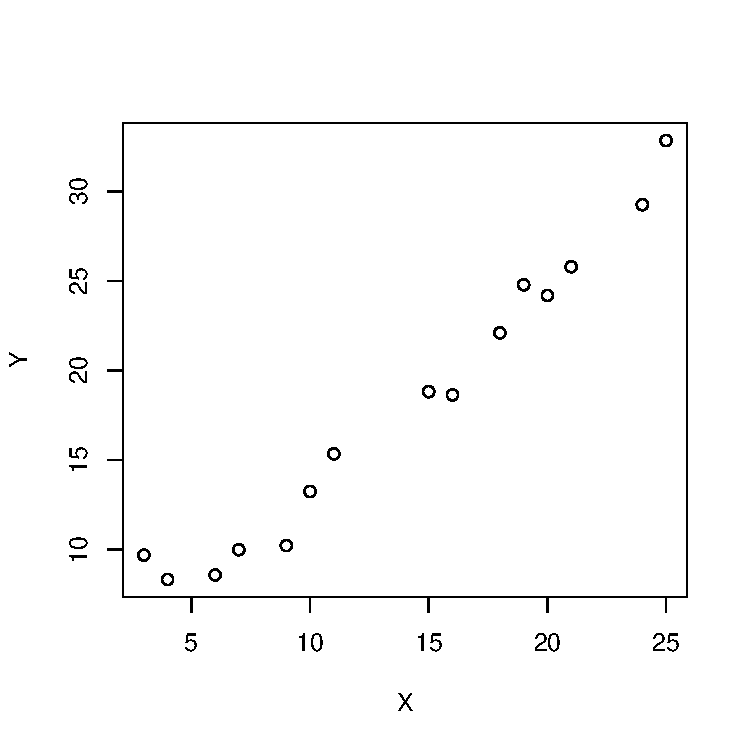
\includegraphics[width=.45\linewidth]{figure/fig-unnamed-chunk-36-1}

}



\end{knitrout}
      \caption{Graphique des données de l'exercice
        \ref{chap:multiple}.\ref{ex:multiple:quadratique}}
      \label{fig:multiple:quadratique}
    \end{figure}
    Par la suite, on peut estimer les paramètres de ce modèle avec la
    fonction \texttt{lm} de \textsf{R}:
\begin{knitrout}
\definecolor{shadecolor}{rgb}{0.969, 0.969, 0.969}\color{fgcolor}\begin{kframe}
\begin{alltt}
\hlstd{fit} \hlkwb{<-} \hlkwd{lm}\hlstd{(Y} \hlopt{~} \hlkwd{poly}\hlstd{(X,} \hlnum{2}\hlstd{),} \hlkwc{data} \hlstd{= donnees)}
\hlkwd{summary}\hlstd{(fit)}
\end{alltt}
\begin{verbatim}
##
## Call:
## lm(formula = Y ~ poly(X, 2), data = donnees)
##
## Residuals:
##     Min      1Q  Median      3Q     Max
## -1.9123 -0.6150 -0.1905  0.6367  1.6921
##
## Coefficients:
##             Estimate Std. Error t value Pr(>|t|)
## (Intercept)  18.1240     0.3025   59.91 3.10e-16 ***
## poly(X, 2)1  29.6754     1.1717   25.33 8.72e-12 ***
## poly(X, 2)2   4.0899     1.1717    3.49  0.00446 **
## ---
## Signif. codes:
## 0 '***' 0.001 '**' 0.01 '*' 0.05 '.' 0.1 ' ' 1
##
## Residual standard error: 1.172 on 12 degrees of freedom
## Multiple R-squared:  0.982,	Adjusted R-squared:  0.979
## F-statistic: 326.8 on 2 and 12 DF,  p-value: 3.434e-11
\end{verbatim}
\begin{alltt}
\hlkwd{anova}\hlstd{(fit)}
\end{alltt}
\begin{verbatim}
## Analysis of Variance Table
##
## Response: Y
##            Df Sum Sq Mean Sq F value    Pr(>F)
## poly(X, 2)  2 897.36  448.68  326.79 3.434e-11 ***
## Residuals  12  16.48    1.37
## ---
## Signif. codes:
## 0 '***' 0.001 '**' 0.01 '*' 0.05 '.' 0.1 ' ' 1
\end{verbatim}
\end{kframe}
\end{knitrout}
    Tant le test $F$ global que les tests $t$ individuels sont
    concluants, le coefficient de détermination est élevé et l'on peut
    constater à la figure \ref{fig:multiple:quadratique2} que
    l'ajustement du modèle est bon. On conclut donc qu'un modèle
    adéquat pour cet ensemble de données est
    \begin{displaymath}
      Y_t = 18,12 +
      29,68 X_t +
      4,09 X_t^2 + \varepsilon_t, \quad
      \varepsilon_t \sim N(0, 1,373).
    \end{displaymath}
    \begin{figure}
      \centering
\begin{knitrout}
\definecolor{shadecolor}{rgb}{0.969, 0.969, 0.969}\color{fgcolor}\begin{kframe}
\begin{alltt}
\hlkwd{plot}\hlstd{(Y} \hlopt{~} \hlstd{X,} \hlkwc{data} \hlstd{= donnees)}
\hlstd{x} \hlkwb{<-} \hlkwd{seq}\hlstd{(}\hlkwd{min}\hlstd{(donnees}\hlopt{$}\hlstd{X),} \hlkwd{max}\hlstd{(donnees}\hlopt{$}\hlstd{X),} \hlkwc{length} \hlstd{=} \hlnum{200}\hlstd{)}
\hlkwd{lines}\hlstd{(x,} \hlkwd{predict}\hlstd{(fit,} \hlkwd{data.frame}\hlstd{(}\hlkwc{X} \hlstd{= x),} \hlkwc{lwd} \hlstd{=} \hlnum{2}\hlstd{))}
\end{alltt}
\end{kframe}

{\centering 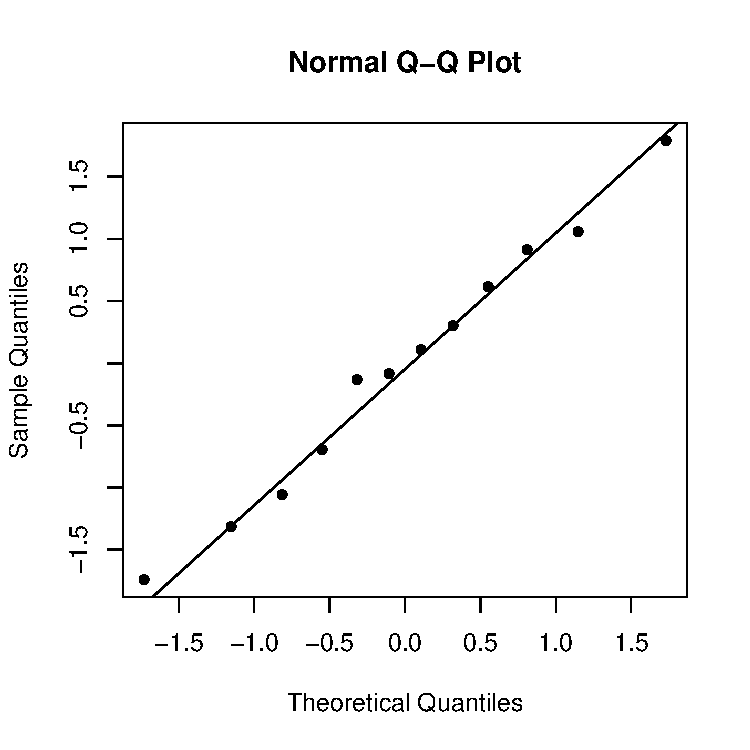
\includegraphics[width=.45\linewidth]{figure/fig-unnamed-chunk-38-1}

}



\end{knitrout}
      \caption{Graphique des données de l'exercice
        \ref{chap:multiple}.\ref{ex:multiple:quadratique} et courbe
        obtenue par régression}
      \label{fig:multiple:quadratique2}
    \end{figure}
  
\end{solution}
\begin{solution}{3.17}
    Comme on peut le constater à la figure \ref{fig:multiple:pondere},
    le point $(X_{16}, Y_{16})$ est plus éloigné des autres. En b) et
    c), on diminue son poids dans la régression.
    \begin{figure}
      \centering
\begin{knitrout}
\definecolor{shadecolor}{rgb}{0.969, 0.969, 0.969}\color{fgcolor}\begin{kframe}
\begin{alltt}
\hlkwd{plot}\hlstd{(Y} \hlopt{~} \hlstd{X,} \hlkwc{data} \hlstd{= donnees)}
\hlkwd{points}\hlstd{(donnees}\hlopt{$}\hlstd{X[}\hlnum{16}\hlstd{], donnees}\hlopt{$}\hlstd{Y[}\hlnum{16}\hlstd{],} \hlkwc{pch} \hlstd{=} \hlnum{16}\hlstd{)}
\end{alltt}
\end{kframe}

{\centering \includegraphics[width=.45\linewidth]{figure/fig-unnamed-chunk-40-1}

}



\end{knitrout}
      \caption{Graphique des données de l'exercice
        \ref{chap:multiple}.\ref{ex:multiple:pondere}. Le cercle plein
        représente la donnée $(X_{16}, Y_{16})$.}
      \label{fig:multiple:pondere}
    \end{figure}
    \begin{enumerate}
    \item On calcule d'abord l'estimateur des moindres carrés ordinaires:
\begin{knitrout}
\definecolor{shadecolor}{rgb}{0.969, 0.969, 0.969}\color{fgcolor}\begin{kframe}
\begin{alltt}
\hlstd{(fit1} \hlkwb{<-} \hlkwd{lm}\hlstd{(Y} \hlopt{~} \hlstd{X,} \hlkwc{data} \hlstd{= donnees))}
\end{alltt}
\begin{verbatim}
##
## Call:
## lm(formula = Y ~ X, data = donnees)
##
## Coefficients:
## (Intercept)            X
##      1.4256       0.3158
\end{verbatim}
\end{kframe}
\end{knitrout}
    \item Si l'on suppose que la variance de la données $(X_{16},
      Y_{16})$ est quatre fois plus élevée que la variance des autres
      données, alors il convient d'accorder un point quatre fois moins
      grand à cette donnée dans la régression. Cela requiert les
      moindres carrés pondérés. Pour calculer les estimateurs avec
      \texttt{lm} dans \textsf{R}, on utilise l'argument
      \texttt{weights}:
\begin{knitrout}
\definecolor{shadecolor}{rgb}{0.969, 0.969, 0.969}\color{fgcolor}\begin{kframe}
\begin{alltt}
\hlstd{w} \hlkwb{<-} \hlkwd{rep}\hlstd{(}\hlnum{1}\hlstd{,} \hlkwd{nrow}\hlstd{(donnees))}
\hlstd{w[}\hlnum{16}\hlstd{]} \hlkwb{<-} \hlnum{0.25}
\hlstd{(fit2} \hlkwb{<-} \hlkwd{update}\hlstd{(fit1,} \hlkwc{weights} \hlstd{= w))}
\end{alltt}
\begin{verbatim}
##
## Call:
## lm(formula = Y ~ X, data = donnees, weights = w)
##
## Coefficients:
## (Intercept)            X
##      1.7213       0.2243
\end{verbatim}
\end{kframe}
\end{knitrout}
    \item On répète la procédure en b) avec un poids de encore plus
      petit pour la donnée $(X_{16}, Y_{16})$:
\begin{knitrout}
\definecolor{shadecolor}{rgb}{0.969, 0.969, 0.969}\color{fgcolor}\begin{kframe}
\begin{alltt}
\hlstd{w[}\hlnum{16}\hlstd{]} \hlkwb{<-} \hlnum{0.0625}
\hlstd{(fit3} \hlkwb{<-} \hlkwd{update}\hlstd{(fit1,} \hlkwc{weights} \hlstd{= w))}
\end{alltt}
\begin{verbatim}
##
## Call:
## lm(formula = Y ~ X, data = donnees, weights = w)
##
## Coefficients:
## (Intercept)            X
##      1.8080       0.1975
\end{verbatim}
\end{kframe}
\end{knitrout}
      Plus le poids accordé à la donnée $(X_{16}, Y_{16})$ est faible,
      moins la droite de régression est attirée vers ce point (voir la
      figure \ref{fig:multiple:pondere2}).
      \begin{figure}[t]
        \centering
\begin{knitrout}
\definecolor{shadecolor}{rgb}{0.969, 0.969, 0.969}\color{fgcolor}\begin{kframe}
\begin{alltt}
\hlkwd{plot}\hlstd{(Y} \hlopt{~} \hlstd{X,} \hlkwc{data} \hlstd{= donnees)}
\hlkwd{points}\hlstd{(donnees}\hlopt{$}\hlstd{X[}\hlnum{16}\hlstd{], donnees}\hlopt{$}\hlstd{Y[}\hlnum{16}\hlstd{],} \hlkwc{pch} \hlstd{=} \hlnum{16}\hlstd{)}
\hlkwd{abline}\hlstd{(fit1,} \hlkwc{lwd} \hlstd{=} \hlnum{2}\hlstd{,} \hlkwc{lty} \hlstd{=} \hlnum{1}\hlstd{)}
\hlkwd{abline}\hlstd{(fit2,} \hlkwc{lwd} \hlstd{=} \hlnum{2}\hlstd{,} \hlkwc{lty} \hlstd{=} \hlnum{2}\hlstd{)}
\hlkwd{abline}\hlstd{(fit3,} \hlkwc{lwd} \hlstd{=} \hlnum{2}\hlstd{,} \hlkwc{lty} \hlstd{=} \hlnum{3}\hlstd{)}
\hlkwd{legend}\hlstd{(}\hlnum{1.2}\hlstd{,} \hlnum{6}\hlstd{,} \hlkwc{legend} \hlstd{=} \hlkwd{c}\hlstd{(}\hlstr{"Modèle a)"}\hlstd{,} \hlstr{"Modèle b)"}\hlstd{,} \hlstr{"Modèle c)"}\hlstd{),}
       \hlkwc{lwd} \hlstd{=} \hlnum{2}\hlstd{,} \hlkwc{lty} \hlstd{=} \hlnum{1}\hlopt{:}\hlnum{3}\hlstd{)}
\end{alltt}
\end{kframe}

{\centering \includegraphics[width=.45\linewidth]{figure/fig-unnamed-chunk-44-1}

}



\end{knitrout}
        \caption{Graphique des données de l'exercice
          \ref{chap:multiple}.\ref{ex:multiple:pondere} avec les
          droites de régression obtenues à l'aide des moindres carrés
          pondérés.}
        \label{fig:multiple:pondere2}
      \end{figure}
    \end{enumerate}
  
\end{solution}
\begin{solution}{3.18}
    \begin{enumerate}
    \item Voir la figure \ref{fig:multiple:taxi} pour le graphique. Il
      y a effectivement une différence entre la consommation de
      carburant des hommes et des femmes: ces dernières font plus de
      milles avec un gallon d'essence.
      \begin{figure}
        \centering
\begin{knitrout}
\definecolor{shadecolor}{rgb}{0.969, 0.969, 0.969}\color{fgcolor}\begin{kframe}
\begin{alltt}
\hlstd{hommes} \hlkwb{<-} \hlkwd{subset}\hlstd{(donnees, sexe} \hlopt{==} \hlstr{"M"}\hlstd{)}
\hlstd{femmes} \hlkwb{<-} \hlkwd{subset}\hlstd{(donnees, sexe} \hlopt{==} \hlstr{"F"}\hlstd{)}
\hlkwd{plot}\hlstd{(mpg} \hlopt{~} \hlstd{age,} \hlkwc{data} \hlstd{= hommes,}
     \hlkwc{xlim} \hlstd{=} \hlkwd{range}\hlstd{(donnees}\hlopt{$}\hlstd{age),} \hlkwc{ylim} \hlstd{=} \hlkwd{range}\hlstd{(donnees}\hlopt{$}\hlstd{mpg))}
\hlkwd{points}\hlstd{(mpg} \hlopt{~} \hlstd{age,} \hlkwc{data} \hlstd{= femmes,} \hlkwc{pch} \hlstd{=} \hlnum{16}\hlstd{)}
\hlkwd{legend}\hlstd{(}\hlnum{4}\hlstd{,} \hlnum{16}\hlstd{,} \hlkwc{legend} \hlstd{=} \hlkwd{c}\hlstd{(}\hlstr{"Hommes"}\hlstd{,} \hlstr{"Femmes"}\hlstd{),} \hlkwc{pch} \hlstd{=} \hlkwd{c}\hlstd{(}\hlnum{1}\hlstd{,} \hlnum{16}\hlstd{))}
\end{alltt}
\end{kframe}

{\centering \includegraphics[width=.45\linewidth]{figure/fig-unnamed-chunk-46-1}

}



\end{knitrout}
        \caption{Graphique des données de l'exercice
          \ref{chap:multiple}.\ref{ex:multiple:taxi}}
        \label{fig:multiple:taxi}
      \end{figure}
    \item Remarquer que la variable \texttt{sexe} est un facteur et peut
      être utilisée telle quelle dans \texttt{lm}:
\begin{knitrout}
\definecolor{shadecolor}{rgb}{0.969, 0.969, 0.969}\color{fgcolor}\begin{kframe}
\begin{alltt}
\hlstd{(fit} \hlkwb{<-} \hlkwd{lm}\hlstd{(mpg} \hlopt{~} \hlstd{age} \hlopt{+} \hlstd{sexe,} \hlkwc{data} \hlstd{= donnees))}
\end{alltt}
\begin{verbatim}
##
## Call:
## lm(formula = mpg ~ age + sexe, data = donnees)
##
## Coefficients:
## (Intercept)          age        sexeM
##      16.687       -1.040       -1.206
\end{verbatim}
\end{kframe}
\end{knitrout}
    \item Calcul d'une prévision pour la valeur moyenne de la variable
      \texttt{mpg}:
\begin{knitrout}
\definecolor{shadecolor}{rgb}{0.969, 0.969, 0.969}\color{fgcolor}\begin{kframe}
\begin{alltt}
\hlkwd{predict}\hlstd{(fit,} \hlkwc{newdata} \hlstd{=} \hlkwd{data.frame}\hlstd{(}\hlkwc{age} \hlstd{=} \hlnum{4}\hlstd{,} \hlkwc{sexe} \hlstd{=} \hlstr{"F"}\hlstd{),}
        \hlkwc{interval} \hlstd{=} \hlstr{"confidence"}\hlstd{,} \hlkwc{level} \hlstd{=} \hlnum{0.90}\hlstd{)}
\end{alltt}
\begin{verbatim}
##        fit      lwr      upr
## 1 12.52876 11.94584 13.11168
\end{verbatim}
\end{kframe}
\end{knitrout}
    \end{enumerate}
  
\end{solution}
\begin{solution}{3.19}
\begin{enumerate}
\item Le postulat de normalité semble violé.

La distribution des résidus a une queue inférieure plus épaisse que la loi normale, ce que l'on voit à gauche du Q-Q plot, puisque les poits ne sont pas alignés.

Le postulat de normalité n'est pas critique, parce que les estimateurs des moindres carrés ont un sens quand même. Toutefois, les tests d'hypothèses et les intervalles de confiance ne sont pas valides.

\item Le graphique des résidus en fonction de $x_2$ montre que le postulat de linéarité semble violé. Cela implique que le modèle n'est pas valide.

On observe de l'hétéroscédasticité (par exemple, dans les graphiques 1, 3 ou 4) puisque les résidus ne semblent pas avoir une variance constante.

Cela signifie que les variances des paramètres ne sont pas calculées de façon appropriée OU il faudrait effectuer une transformation sur les variables pour régler ces problèmes.


\end{enumerate}
\end{solution}
\begin{solution}{3.20}
On pourrait croire qu'un point sur 20, ça ne change rien, mais ce n'est pas le cas! Le point 1 a un impact sur la pente et la qualité de l'ajustement. Le point 2 a un grand levier mais n'affecte pas beaucoup les estimations, le point 3 a un grand levier et un gros impact.

\begin{verbatim}
dat <- read.csv("OutlierExample.csv")

dim(dat)

summary(dat)

library(ggplot2)

ggplot(dat, aes(x= X, y= Y, label=CODES))+
  geom_point() +
  geom_text(aes(label=ifelse(CODES>0,CODES,'')),hjust=0,vjust=0)

fit0 <- lm(Y~X,dat,subset=(CODES==0))
summary(fit0)
plot(dat[,1:2],pch=16)
points(dat[match(1:3,dat$CODES),1:2],col=2:4,pch=16:18,cex=1.2)
abline(fit0)

fit1 <- lm(Y~X,dat,subset=(CODES<=1))
summary(fit1)
abline(fit1,col=2,lty=2)

fit2 <- lm(Y~X,dat,subset=(CODES%in%c(0,2)))
summary(fit2)
abline(fit2,col=3,lty=3)

fit3 <- lm(Y~X,dat,subset=(CODES%in%c(0,3)))
summary(fit3)
abline(fit3,col=4,lty=4)

influence.measures(fit0)
influence.measures(fit1)
influence.measures(fit2)
influence.measures(fit3)

\end{verbatim}
\end{solution}

\newpage
\section*{Chapitre \ref{chap:selection}}
\addcontentsline{toc}{section}{Chapitre \protect\ref{chap:selection}}

\begin{solution}{2.1}
\begin{enumerate}
\item
\begin{enumerate}
\item modèle D
\item modèle D
\item modèle G
\item modèle G
\item modèle C
\item modèle H
\end{enumerate}

\item Il y a un très gros problème de multicolinéarité pour les modèle F, G et H, car certains VIFs sont beaucoup plus grands que 10. Ce problème augmente inutilement la variance des paramètres estimés.

\item On évite les modèles F G et H pour ne pas avoir de problème de multicolinéarité. Le modèle D est préférable selon les critères PRESS et $R^2_p$. De plus, ses critères AIC et BIC sont les deuxièmes plus petits. Le $C_p$ est 8, donc 8-5=3. Ce n'est pas parfait, mais ce n'est pas si mal, etc.

\end{enumerate}
\end{solution}
\begin{solution}{2.2}
\begin{enumerate}
\item Puisque $n=p$, $\beta_0=0$ et que la matrice d'incidence est diagonale, on a $\hat{y}_i = \hat\beta_i$ pour $i=1,\ldots,n$. On minimise $S(\bobeta)=\sum_{i=1}^n (y_i-\beta_i)^2$ et on trouve pour $i\in \{1,\ldots,n\}$,
$$
\left.\frac{\partial}{\partial\beta_i}S(\bobeta)\right|_{\hat\beta_i}= -2 (y_i-\hat\beta_i) =0 \quad \Rightarrow \quad \hat\beta_i =  y_i.
$$

\item On minimise, pour une valeur $\lambda>0$,
$$
S^{\mathrm{ridge}}(\bobeta)=\sum_{i=1}^n (y_i-\beta_i)^2 +\lambda \sum_{i=1}^n \beta_i^2.
$$

\item On a
$$
\frac{\partial}{\partial\beta_i}S^{\mathrm{ridge}}(\bobeta)=-2(y_i-\beta_i) +2 \lambda  \beta_i.
$$
On pose égal à 0 et on trouve
$$
y_i-\hat \beta_i^{\mathrm{ridge}} = \lambda  \hat\beta_i^{\mathrm{ridge}} \quad \Rightarrow \quad \hat\beta_i^{\mathrm{ridge}} =  \frac{y_i}{1+\lambda}.
$$

\item On minimise, pour une valeur $\lambda>0$,
$$
S^{\mathrm{lasso}}(\bobeta)=\sum_{i=1}^n (y_i-\beta_i)^2 +\lambda \sum_{i=1}^n |\beta_i|.
$$

\item On a
$$
\frac{\partial}{\partial\beta_i}S^{\mathrm{lasso}}(\bobeta)=-2(y_i-\beta_i) + \lambda\, \mathrm{signe}(\beta_i) .
$$
On utilise les EMV trouvés en a) pour définir le signe. Supposons d'abord que $\hat\beta_i = y_i>0$. Alors, on a aussi $\hat\beta_i^{\mathrm{lasso}}>0$ (sinon, changer le signe donnera une valeur plus petite de l'équation à minimiser). On pose la dérivée égale à 0 et on trouve
$$
2(y_i-\hat \beta_i^{\mathrm{lasso}}) = \lambda  \quad \Rightarrow \quad \hat\beta_i^{\mathrm{ridge}} =  y_i- \lambda/2,
$$
ce qui tient seulement si $\hat\beta_i^{\mathrm{lasso}}>0$, alors on a $\hat\beta_i^{\mathrm{ridge}} =  \max(0,y_i- \lambda/2)$.
Supposons ensuite que $\hat \beta_i = y_i <0$. Alors, on a aussi $\hat\beta_i^{\mathrm{lasso}}<0$. On pose la dérivée égale à 0 et on trouve
$$
2(y_i-\hat \beta_i^{\mathrm{lasso}}) = -\lambda  \quad \Rightarrow \quad \hat\beta_i^{\mathrm{ridge}} =  y_i+ \lambda/2,
$$
sous la contrainte que ce soit négatif, donc dans ce cas, $\hat\beta_i^{\mathrm{ridge}} =  \min(0,y_i+\lambda/2)$. On combine les deux cas et on obtient l'équation donnée.

\item On peut voir que la façon de rapetisser les paramètres est bien différente pour les deux méthodes. Avec ridge, chaque coefficient des moindres carrés est réduit par la même proportion. Avec lasso, chaque coefficient des moindres carrés est réduit vers 0 d'un montant constant $\lambda/2$; ceux qui sont plus petits que $\lambda/2$ en valeur absolue sont mis exactement égaux à 0. C'est de cette façon que le lasso permet de faire la sélection des variables explicatives.

\end{enumerate}
\end{solution}

\newpage
\section*{Chapitre \ref{chap:glm}}
\addcontentsline{toc}{section}{Chapitre \protect\ref{chap:glm}}

\begin{solution}{5.1}
\begin{enumerate}
\item Normale$(\mu,\sigma^2)$: oui,
\begin{align*}
f_{Y}(y)&=\frac{1}{(2\pi\sigma^2)^1/2}\exp\left(-\frac{(y-\mu)^2}{2\sigma^2}\right),\, y\in\mathbb{R}\\
&=\exp\left(\frac{y\mu-\mu^2/2}{\sigma^2}-\frac{y^2}{2\sigma^2}-\frac{\ln(2\pi\sigma^2)}{2}\right),\, y\in\mathbb{R}.
\end{align*}
\begin{itemize}
\item[$\bullet$] Paramètre canonique: $\theta=\mu$
\item[$\bullet$] Paramètre de dispersion: $\phi=\sigma^2$
\item[$\bullet$] $b(\theta)=\frac{\theta^2}{2}$
\item[$\bullet$] $E[Y]=\dot{b}(\theta)=\frac{\partial}{\partial\theta}\frac{\theta^2}{2}=\theta=\mu$
\item[$\bullet$] $\var(Y)=\phi\ddot{b}(\theta)=\sigma^2\frac{\partial}{\partial\theta}\theta=\sigma^2$
\item[$\bullet$] $V(\mu)=1$.
\end{itemize}

\item Uniforme$(0,\beta)$: non. Le domaine dépend du paramètre $\beta$.
\item Poisson$(\lambda)$:
\begin{align*}
f_{Y}(y;\lambda)&=\frac{\lambda^{y}e^{-\lambda}}{y!} \mbox{, pour }y\in \mathbb{N}^{+}\\
&=\exp\{y\ln \lambda - \lambda - \ln y!\}\\
f_{Y}(y;\theta,\phi)&=\exp\left\{\frac{y\theta - e^{\theta}}{\phi} - \ln y!\right\}.
\end{align*}
\begin{itemize}
\item[$\bullet$] Paramètre canonique: $\theta=\ln \lambda$
\item[$\bullet$] Paramètre de dispersion: $\phi=1$
\item[$\bullet$] $b(\theta)=e^{\theta}$
\item[$\bullet$] $E[Y]=\dot{b}(\theta)=\frac{\partial}{\partial\theta}e^{\theta}=e^{\theta}=\lambda$
\item[$\bullet$] $\var(Y)=\phi\ddot{b}(\theta)=\frac{\partial}{\partial\theta}e^{\theta}=e^{\theta}=\lambda$
\item[$\bullet$] $V(\mu)=\mu$.
\end{itemize}

\item Bernoulli$(\pi)$
\begin{align*}
f_{Y}(y;\pi)&=\pi^{y}(1-\pi)^{1-y}1(y \in \{0,1\})\\
&=\exp\left\{y\ln\left(\frac{\pi}{1-\pi}\right)+\ln(1-\pi)\right\}1(y \in \{0,1\}).\\
\end{align*}
\begin{itemize}
\item[$\bullet$] Paramètre canonique: $\theta=\ln\left(\frac{\pi}{1-\pi}\right)$
\item[$\bullet$] Paramètre de dispersion:  $\phi=1$
\item[$\bullet$] $b(\theta)=\ln(1+e^{\theta})$
\item[$\bullet$] $E[Y]=\dot{b}(\theta)=\frac{\partial}{\partial\theta}\ln(1+e^{\theta})=\frac{e^{\theta}}{1+e^\theta}=\pi$
\item[$\bullet$] $\var(Y)=\phi\ddot{b}(\theta)=\frac{\partial}{\partial\theta}\frac{e^{\theta}}{1+e^\theta}=\frac{e^\theta}{(1+e^\theta)^2}=\pi(1-\pi)$
\item[$\bullet$] $V(\mu)=\mu(1-\mu)$.
\end{itemize}

\item Binomiale$(m, \pi)$, $m>0$ est un entier et est connu.
\begin{align*}
f_{Y}(y;\pi)&=\begin{pmatrix} m\\y\end{pmatrix}\pi^{y}(1-\pi)^{m-y}1(y \in \{0,1,...,m\})\\
&=\exp\left\{y\ln\left(\frac{\pi}{1-\pi}\right)+m\ln(1-\pi)+\ln\begin{pmatrix} m\\y\end{pmatrix}\right\}1(y \in \{0,1,...,m\}).\\
\end{align*}
Dans cette représentation, on a $$E[Y]=m\pi \mbox{ et } Var(Y)=m\pi(1-\pi).$$ Cette forme est moins utilisée car l'espérance de $Y$ dépend de $m$, le paramètre de dispersion. Souvent, on transforme les données. On utilise plutôt $Y^{*}=Y/m$. Alors, pour ces données transformées,
\begin{align*}
f_{Y^{*}}(y;\pi)&=\exp\left\{my\ln\left(\frac{\pi}{1-\pi}\right)+m\ln(1-\pi)+\ln\begin{pmatrix} m\\my\end{pmatrix}\right\}, \,y \in \{0,1/m,...,1\}\\
&=\exp\left\{\frac{y\ln\left(\frac{\pi}{1-\pi}\right)+\ln(1-\pi)}{1/m}+\ln\begin{pmatrix} m\\my\end{pmatrix}\right\}, \,y \in \{0,1/m,...,1\}.\\
\end{align*}
\begin{itemize}
\item[$\bullet$] Paramètre canonique: $\theta=\ln\left(\frac{\pi}{1-\pi}\right)$
\item[$\bullet$] Paramètre de dispersion:  $\phi=1/m$
\item[$\bullet$] $b(\theta)=\ln(1+e^{\theta})$
\item[$\bullet$] $E[Y^*]=\dot{b}(\theta)=\frac{\partial}{\partial\theta}\ln(1+e^{\theta})=\frac{e^{\theta}}{1+e^\theta}=\pi$
\item[$\bullet$] $\var(Y^*)=\phi\ddot{b}(\theta)=\frac{1}{m}\frac{\partial}{\partial\theta}\frac{e^{\theta}}{1+e^\theta}=\frac{e^\theta}{m(1+e^\theta)^2}=\frac{\pi(1-\pi)}{m}$
\item[$\bullet$] $V(\mu)=\mu(1-\mu)$.
\end{itemize}

\item Pareto$(\alpha,\lambda)$: non.
\item Gamma$(\alpha,\beta)$
Soit $Y\sim Gamma(\alpha,\beta)$. Alors, avec un peu de travail, la densité peut être écrite sous la forme exponentielle linéaire.
$$f_{Y}(y;\alpha,\beta)=\frac{\beta^{\alpha}}{\Gamma(\alpha)}y^{\alpha-1}e^{-\beta y},$$ pour $y>0$. On reparamétrise: $\mu=\alpha/\beta=E[Y]$ et $\alpha$, on a donc $\beta=\alpha/\mu$ et $$f_{Y}(y;\alpha,\mu)=\frac{1}{y\Gamma(\alpha)}\left(\frac{\alpha y}{\mu}\right)^{\alpha}\exp\left\{-\frac{\alpha y}{\mu}\right\}.$$ Posons $\theta=-1/\mu$, et $a(\phi)=1/\alpha$, alors on trouve $$f_{Y}(y;\theta,\phi)=\exp\left\{\frac{y\theta +\ln(-\theta)}{\phi} +\alpha\ln\alpha+(\alpha-1)\ln y -\ln\Gamma(\alpha)\right\}.$$ Donc, $b(\theta)=-\ln(-\theta)$ et $a(\phi)=1/\alpha \Rightarrow \dot{b}(\theta)=\frac{-1}{\theta}=\mu$ et $\ddot{b}(\theta)=\frac{1}{\theta^{2}}=\mu^{2}$. Finalement, $$E[Y]=\frac{-1}{\theta}=\mu \mbox{ et } Var(Y)=\frac{1}{\alpha}\mu^{2}.$$

\item Binomiale négative$(r,\pi)$ avec $r$ connu. On considère $Y^*=Y/r$:
\begin{align*}
f_Y^*(y)&=\begin{pmatrix} r+ry-1\\ry\end{pmatrix}\pi^r(1-\pi)^{ry}, \mbox{ pour } y\in \{0,\frac{1}{r},\frac{2}{r},...\}\\
&=\exp\left(ry\ln(1-\pi)+r\ln\pi+\ln\begin{pmatrix} r+ry-1\\ry\end{pmatrix}\right).
\end{align*}
\begin{itemize}
\item[$\bullet$] Paramètre canonique: $\theta=\ln(1-\pi)$
\item[$\bullet$] Paramètre de dispersion:  $\phi=1/r$
\item[$\bullet$] $b(\theta)=-\ln(1-e^\theta)$
\item[$\bullet$] $E[Y^*]=\dot{b}(\theta)=\frac{\partial}{\partial\theta}-\ln(1-e^\theta)=\frac{e^{\theta}}{1-e^\theta}=\frac{1-\pi}{\pi}$
\item[$\bullet$] $\var(Y^*)=\phi\ddot{b}(\theta)=\frac{1}{r}\frac{\partial}{\partial\theta}\frac{e^{\theta}}{1-e^\theta}=\frac{e^\theta}{r(1-e^\theta)^2}=\frac{(1-\pi)}{r\pi^2}$
\item[$\bullet$] $V(\mu)=\mu(\mu+1)$.
\end{itemize}
\end{enumerate}
\end{solution}
\begin{solution}{5.2}
Le lien canonique est le lien log: $\eta=\ln(\mu)$. On pourrait aussi utiliser d'autres fonctions de lien, telle que le lien identité $\eta=\mu$, le lien inverse $\eta=\frac{1}{\mu}$, mais le lien log est le plus approprié parce que son utilisation garantit une moyenne $\mu$ positive, ce qui est nécessaire pour la loi de Poisson.
\end{solution}
\begin{solution}{5.3}
Le lien canonique pour la loi Gamma est le lien inverse $\eta=1/\mu$. Comme la moyenne d'une loi Gamma est toujours positive, ce lien n'est pas toujours approprié parce qu'il ne restreint pas le domaine de $\mu$ aux réels positifs. Le lien log serait plus approprié dans certains cas.
\end{solution}
\begin{solution}{5.4}
\begin{enumerate}
\item $\eta=g(\mu)=\ln(\mu)$
\item On a $$\ln(\mu_i)=\eta_i=\beta_0+\beta_1x_i.$$ La densité de la loi Poisson est
\begin{align*}
f_{Y_i}(y_i;\mu_i)&=\exp\left(y_i\ln\mu_i-\mu_i-\ln y_i!\right)\\
f_{Y_i}(y_i;\beta_0,\beta_1)&=\exp\left(y_i(\beta_0+\beta_1x_i)-e^{\beta_0+\beta_1x_i}-\ln y_i!\right).
\end{align*}
La fonction de vraisemblance et la log-vraisemblance sont donc:
\begin{align*}
\mathcal{L}(\beta_0,\beta_1)&=\prod_{i=1}^n f_{Y_i}(y_i;\beta_0,\beta_1)=\prod_{i=1}^n\exp\left(y_i(\beta_0+\beta_1x_i)-e^{\beta_0+\beta_1x_i}-\ln y_i!\right)\\
\ell(\beta_0,\beta_1)&=\sum_{i=1}^n y_i(\beta_0+\beta_1x_i)-e^{\beta_0+\beta_1x_i}+\mbox{constante}.
\end{align*}
On maximise la log-vraisemblance:
\begin{align*}
\frac{\partial}{\partial\beta_0}\ell(\beta_0,\beta_1)&=\sum_{i=1}^n y_i-e^{\beta_0+\beta_1x_i}\\
\frac{\partial}{\partial\beta_1}\ell(\beta_0,\beta_1)&=\sum_{i=1}^n y_ix_i-x_i e^{\beta_0+\beta_1x_i}\\
\end{align*}
Donc, les équations à résoudre sont
\begin{align*}
\sum_{i=1}^n y_i-e^{\beta_0+\beta_1x_i}&=0\\
\sum_{i=1}^n x_i(y_i-e^{\beta_0+\beta_1x_i})&=0.\\
\end{align*}
\end{enumerate}
\end{solution}
\begin{solution}{5.5}
La déviance est $$D(y;\hat{\mu})=2(\ell_n(\tilde{\theta})-\ell_n(\hat{\theta})).$$ Pour le modèle Binomial, on a que
\begin{align*}
\ell_n(\theta)&=\sum_{i=1}^n\frac{y_i\ln\left(\frac{\mu_i}{1-\mu_i}\right)+\ln(1-\mu_i)}{1/m_i}.
\end{align*} Alors, dans le modèle complet, $\mu_i=y_i$ et on trouve
\begin{align*}
\ell_n(\tilde{\theta})&=\sum_{i=1}^n\frac{y_i\ln\left(\frac{y_i}{1-y_i}\right)+\ln(1-y_i)}{1/m_i}.
\end{align*}
Dans le modèle développé avec le lien log, $\mu_i=\hat{\mu}_i$ et on trouve
\begin{align*}
\ell_n(\hat{\theta})&=\sum_{i=1}^n\frac{y_i\ln\left(\frac{\hat{\mu}_i}{1-\hat{\mu}_i}\right)+\ln(1-\hat{\mu}_i)}{1/m_i}.
\end{align*}
Finalement, la déviance est
\begin{align*}
D(y;\hat{\mu})&=\sum_{i=1}^n\frac{y_i\ln\left(\frac{y_i}{1-y_i}\right)+\ln(1-y_i)}{1/m_i}-\frac{y_i\ln\left(\frac{\hat{\mu}_i}{1-\hat{\mu}_i}\right)+\ln(1-\hat{\mu}_i)}{1/m_i}\\
&=\sum_{i=1}^n m_i\left[y_i\ln\left(\frac{y_i}{\hat{\mu}_i}\right)+(1-y_i)\ln\left(\frac{1-y_i}{1-\hat{\mu}_i}\right)\right].
\end{align*}
\end{solution}
\begin{solution}{5.6}
Pour la distribution Gamma, on a $V(t)=t^2$ et $b(t)=-\ln(-t)$.

Résidus de Pearson: $$r_{P_i}=\frac{y_i-\hat{\mu}_i}{\sqrt{\hat{\mu}_i^2}}=\frac{y_i-\hat{\mu}_i}{\hat{\mu}_i}.$$
Résidus d'Anscombe:
\begin{align*}
A(t)&=\int_{0}^{t} \frac{\mbox{d}s}{s^{2/3}}=3t^{1/3}\\
\dot{A}(t)&=\frac{1}{s^{2/3}}\\
r_{A_i}&=\frac{A(y_i)-A(\hat{\mu}_i)}{\dot{A}(\hat{\mu}_i)\sqrt{V(\hat{\mu}_i)}}=\frac{3(y_i^{1/3}-\hat{\mu}_i^{1/3})}{\hat{\mu}_i^{1/3}}.
\end{align*}
Résidus de déviance:
\begin{align*}
D_i&=2\left(-\frac{y_i}{y_i}-\ln(y_i)+\frac{y_i}{\hat{\mu}_i}+\ln(\hat{\mu}_i)\right)\\
&=2\left(\ln\left(\frac{\hat{\mu}_i}{y_i}\right)+\frac{y_i-\hat{\mu}_i}{\hat{\mu}_i}\right)\\
r_{D_i}&=sign(y_i-\hat{\mu}_i)\sqrt{2\left(\ln\left(\frac{\hat{\mu}_i}{y_i}\right)+\frac{y_i-\hat{\mu}_i}{\hat{\mu}_i}\right)}.
\end{align*}
\end{solution}
\begin{solution}{5.7}
Cette solution est en anglais, vous pouvez poser vos questions sur le forum, s'il y a lieu.

This is a two-factor model, «Device» takes three levels (M1, M2 and M3) and «Stress» takes 4 levels. The baseline group is M1 device at stress level I. An analysis of deviance is carried out to assess if the parameters for the devices are significant.

\begin{knitrout}
\definecolor{shadecolor}{rgb}{0.969, 0.969, 0.969}\color{fgcolor}\begin{kframe}
\begin{alltt}
\hlstd{glm} \hlkwb{<-} \hlkwd{glm}\hlstd{(Failures}\hlopt{~}\hlstd{Level}\hlopt{*}\hlstd{Machine,}\hlkwc{family}\hlstd{=poisson,}\hlkwc{data}\hlstd{=stresstest)}
\hlkwd{anova}\hlstd{(glm)}
\end{alltt}
\begin{verbatim}
## Analysis of Deviance Table
##
## Model: poisson, link: log
##
## Response: Failures
##
## Terms added sequentially (first to last)
##
##
##               Df Deviance Resid. Df Resid. Dev
## NULL                             11     35.844
## Level          3  20.8567         8     14.987
## Machine        2  12.2154         6      2.772
## Level:Machine  6   2.7719         0      0.000
\end{verbatim}
\begin{alltt}
\hlkwd{qchisq}\hlstd{(}\hlnum{0.95}\hlstd{,} \hlnum{6}\hlstd{)}
\end{alltt}
\begin{verbatim}
## [1] 12.59159
\end{verbatim}
\begin{alltt}
\hlkwd{qchisq}\hlstd{(}\hlnum{0.95}\hlstd{,} \hlnum{2}\hlstd{)}
\end{alltt}
\begin{verbatim}
## [1] 5.991465
\end{verbatim}
\end{kframe}
\end{knitrout}

The model $$\mbox{Stress+Device+Stress.Device}$$ is fitted first. The change in deviance from the simpler model $\mbox{Stress+Device}$ is 2.7719 on 6 degrees of freedom, which is not significant when compared to $\chi^{2}_{(6,0.95)}=12.59$. Hence, the model $\mbox{Stress+Device}$ is an adequate simplification of the more complex model. If we then test for the significance of the Device parameters, we find that the change in deviance from the simpler model Stress is 12.2154 on 2 degrees of freedom, which is significant because $\chi^{2}_{(2,0.95)}=5.99$. From this analysis, we can conclude that there is a significant difference between the failure rates of the different devices.
\end{solution}
\begin{solution}{5.8}
\begin{enumerate}
\item En \texttt{R}, on obtient
\begin{knitrout}
\definecolor{shadecolor}{rgb}{0.969, 0.969, 0.969}\color{fgcolor}\begin{kframe}
\begin{alltt}
\hlstd{modinv} \hlkwb{<-} \hlkwd{glm}\hlstd{(AvCost}\hlopt{~}\hlstd{OwnerAge}\hlopt{+}\hlstd{Model}\hlopt{+}\hlstd{CarAge,}\hlkwc{family}\hlstd{=Gamma,}\hlkwc{data}\hlstd{=Bcar)}
\hlkwd{summary}\hlstd{(modinv)}
\end{alltt}
\begin{verbatim}
##
## Call:
## glm(formula = AvCost ~ OwnerAge + Model + CarAge, family = Gamma,
##     data = Bcar)
##
## Deviance Residuals:
##      Min        1Q    Median        3Q       Max
## -1.85536  -0.13930  -0.00821   0.07444   1.49969
##
## Coefficients:
##                 Estimate Std. Error t value Pr(>|t|)
## (Intercept)    0.0033233  0.0004038   8.230 4.42e-13
## OwnerAge21-24  0.0006043  0.0004159   1.453  0.14908
## OwnerAge25-29  0.0003529  0.0003933   0.897  0.37163
## OwnerAge30-34  0.0011783  0.0004572   2.577  0.01130
## OwnerAge35-39  0.0016372  0.0004990   3.281  0.00139
## OwnerAge40-49  0.0012039  0.0004592   2.622  0.01000
## OwnerAge50-59  0.0010998  0.0004511   2.438  0.01638
## OwnerAge60+    0.0012390  0.0004619   2.682  0.00845
## ModelB        -0.0002817  0.0004049  -0.696  0.48806
## ModelC        -0.0006502  0.0003906  -1.664  0.09893
## ModelD        -0.0018235  0.0003481  -5.239 7.96e-07
## CarAge10+      0.0033776  0.0004747   7.115 1.24e-10
## CarAge4-7      0.0003393  0.0002723   1.246  0.21539
## CarAge8-9      0.0017423  0.0003575   4.873 3.75e-06
##
## (Intercept)   ***
## OwnerAge21-24
## OwnerAge25-29
## OwnerAge30-34 *
## OwnerAge35-39 **
## OwnerAge40-49 **
## OwnerAge50-59 *
## OwnerAge60+   **
## ModelB
## ModelC        .
## ModelD        ***
## CarAge10+     ***
## CarAge4-7
## CarAge8-9     ***
## ---
## Signif. codes:
## 0 '***' 0.001 '**' 0.01 '*' 0.05 '.' 0.1 ' ' 1
##
## (Dispersion parameter for Gamma family taken to be 0.1074529)
##
##     Null deviance: 27.841  on 122  degrees of freedom
## Residual deviance: 11.511  on 109  degrees of freedom
##   (5 observations deleted due to missingness)
## AIC: 1400.7
##
## Number of Fisher Scoring iterations: 5
\end{verbatim}
\end{kframe}
\end{knitrout}

\item On a utilisé un lien inverse, alors $E[Y_i]=\frac{1}{\eta_i}.$ Puisque les variables explicatives prennent toutes leur niveau de base, on a que $\hat{\eta}_i=\hat{\beta}_0=0.0033233$ et $$\widehat{E[Y_i]}=0.0033233^{-1}=300.91.$$

\item Puisqu'on a utilisé un lien inverse, un coefficient plus élevé implique une diminution de l'espérance du coût de la réclamation, alors qu'un coefficient négatif signifie une augmentation de cette espérance. Ici on observe que les sept coefficients sont positifs, alors la catégorie d'âge ayant une espérance de coût la plus élevée est la catégorie de base, 17-20 ans. Le coût moyen semble ensuite relativement élevé pour les jeunes entre 21 et 29 ans. La catégorie d'âge avec coût de réclamation minimal est 35-39 ans, puis la moyenne semble relativement stable pour les détenteurs de police plus âgés.

\item Les trois coefficients pour la variable modèle sont négatifs, ce qui signifie que les réclamations pour les véhicules de type A (niveau de base) sont moins élevées en moyenne que celles pour les autres types de véhicule. Les réclamatios pour les véhicules du modèle D semblent particulièrement coûteuse car le coefficient est beaucoup plus grand en valeur absolue que les autres.

\item De la même façon, on observe que d'augmenter l'âge du véhicule diminue le coût moyen des réclamations.

\item Pour un détenteur de police entre 17 et 20 ans, avec un véhicule de type D âgé de un à 3 ans, on trouve que $$\widehat{E[Y_i]}=\frac{1}{\hat{\beta}_0+\hat{\beta}^{MODEL}_D}=\frac{1}{0.0033233-0.0018235}=666.76.$$

\item Pour un détenteur de police entre 35 et 39 ans, avec un véhicule de type A âgé de plus de 10 ans, on trouve que $$\widehat{E[Y_i]}=\frac{1}{\hat{\beta}_0+\hat{\beta}^{OWNERAGE}_{35-39}+\hat{\beta}^{CARAGE}_{10+}}=\frac{1}{0.0033233+0.0016372+0.0033776}=119.93.$$

\item La déviance $D(y,\hat{\mu})=11.511$ est donnée dans la sortie \texttt{R} pour la sous-question a). On a que $$\frac{D(y,\hat{\mu})}{\hat{\phi}}=\frac{11.511}{0.1074529}=107.126,$$ ce qui est très près de $n-p'=109$. Le modèle semble donc adéquat.

\item Les résidus sont calculés avec les formules trouvées à la question 6. Il faut d'abord enlever les données manquantes du vecteur contenant les coûts moyens. On obtient les graphiques de la Figure~\ref{fig:glm:residuals}.

\begin{figure}
\begin{center}
\begin{knitrout}
\definecolor{shadecolor}{rgb}{0.969, 0.969, 0.969}\color{fgcolor}
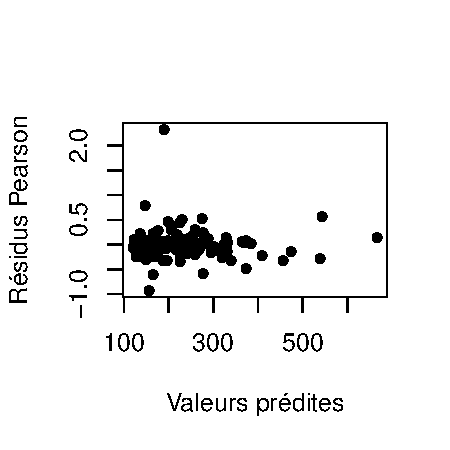
\includegraphics[width=\maxwidth]{figure/unnamed-chunk-75-1}

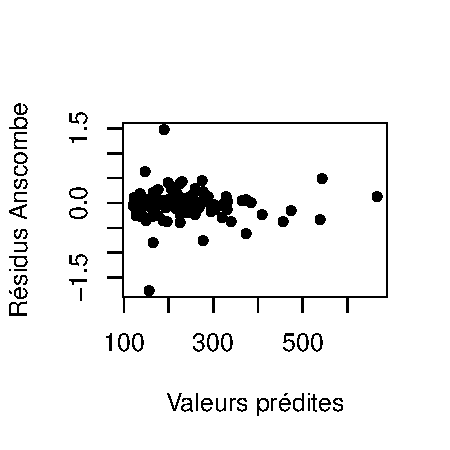
\includegraphics[width=\maxwidth]{figure/unnamed-chunk-75-2}

\includegraphics[width=\maxwidth]{figure/unnamed-chunk-75-3}

\end{knitrout}
\caption{Résidus pour GLM Gamma}\label{fig:glm:residuals}
\end{center}
\end{figure}

\item a. Le modèle avec le lien logarithmique est

\begin{knitrout}
\definecolor{shadecolor}{rgb}{0.969, 0.969, 0.969}\color{fgcolor}\begin{kframe}
\begin{alltt}
\hlstd{modlog} \hlkwb{<-} \hlkwd{glm}\hlstd{(AvCost}\hlopt{~}\hlstd{OwnerAge}\hlopt{+}\hlstd{Model}\hlopt{+}\hlstd{CarAge,}\hlkwc{family}\hlstd{=}\hlkwd{Gamma}\hlstd{(}\hlkwc{link}\hlstd{=log),}\hlkwc{data}\hlstd{=Bcar)}
\hlkwd{summary}\hlstd{(modlog)}
\end{alltt}
\begin{verbatim}
##
## Call:
## glm(formula = AvCost ~ OwnerAge + Model + CarAge, family = Gamma(link = log),
##     data = Bcar)
##
## Deviance Residuals:
##      Min        1Q    Median        3Q       Max
## -1.84819  -0.12796  -0.00834   0.08552   1.20066
##
## Coefficients:
##                Estimate Std. Error t value Pr(>|t|)
## (Intercept)    5.711739   0.103835  55.008  < 2e-16
## OwnerAge21-24 -0.108159   0.114547  -0.944   0.3471
## OwnerAge25-29  0.005223   0.113170   0.046   0.9633
## OwnerAge30-34 -0.288090   0.113170  -2.546   0.0123
## OwnerAge35-39 -0.331420   0.114547  -2.893   0.0046
## OwnerAge40-49 -0.280775   0.113170  -2.481   0.0146
## OwnerAge50-59 -0.238136   0.113170  -2.104   0.0377
## OwnerAge60+   -0.283521   0.113170  -2.505   0.0137
## ModelB         0.057951   0.075447   0.768   0.4441
## ModelC         0.154588   0.076115   2.031   0.0447
## ModelD         0.472290   0.078497   6.017 2.43e-08
## CarAge10+     -0.735513   0.078497  -9.370 1.17e-15
## CarAge4-7     -0.111412   0.075447  -1.477   0.1426
## CarAge8-9     -0.422538   0.076115  -5.551 2.02e-07
##
## (Intercept)   ***
## OwnerAge21-24
## OwnerAge25-29
## OwnerAge30-34 *
## OwnerAge35-39 **
## OwnerAge40-49 *
## OwnerAge50-59 *
## OwnerAge60+   *
## ModelB
## ModelC        *
## ModelD        ***
## CarAge10+     ***
## CarAge4-7
## CarAge8-9     ***
## ---
## Signif. codes:
## 0 '***' 0.001 '**' 0.01 '*' 0.05 '.' 0.1 ' ' 1
##
## (Dispersion parameter for Gamma family taken to be 0.0910768)
##
##     Null deviance: 27.841  on 122  degrees of freedom
## Residual deviance: 11.263  on 109  degrees of freedom
##   (5 observations deleted due to missingness)
## AIC: 1398
##
## Number of Fisher Scoring iterations: 7
\end{verbatim}
\end{kframe}
\end{knitrout}

b. Avec ce modèle $E[Y_i]=e^{\eta_i}.$ Puisque les variables explicatives prennent toutes leur niveau de base, on a que $\hat{\eta}_i=\hat{\beta}_0=5.711739$ et $$\widehat{E[Y_i]}=e^5.711739=302.39.$$ Cela ne diffère pas beaucoup du résultat trouvé en b).

c-d-e. Puisqu'on a utilisé un lien logarithmique, on a un modèle multiplicatif. Si $e^\beta>1$, alors l'espérance du coût augmente, alors que si $e^\beta<1$ alors l'espérance du coût diminue. On peut donc tirer des conclusions similaires à celles en c), d) et e).

f. Pour un détenteur de police entre 17 et 20 ans, avec un véhicule de type D âgé de un à 3 ans, on trouve que $$\widehat{E[Y_i]}=\exp{\hat{\beta}_0+\hat{\beta}^{MODEL}_D}=\exp{5.711739+0.472290}=484.94.$$ On note que cette valeur est beaucoup moins élevée que celle obtenue en f).

g. Pour un détenteur de police entre 35 et 39 ans, avec un véhicule de type A âgé de plus de 10 ans, on trouve que $$\widehat{E[Y_i]}=\exp{\hat{\beta}_0+\hat{\beta}^{OWNERAGE}_{35-39}+\hat{\beta}^{CARAGE}_{10+}}=\exp{5.711739-0.331420-0.735513}=104.04.$$

h. La déviance $D(y,\hat{\mu})=11.263$ est donnée dans la sortie \texttt{R} pour la sous-question a). On a que $$\frac{D(y,\hat{\mu})}{\hat{\phi}}=\frac{11.263}{0.0910768}=123.66,$$ ce qui est moins près de $n-p'=109$ que pour le modèle avec le lien inverse. Le modèle semble donc moins adéquat.
\end{enumerate}
\end{solution}
\begin{solution}{5.9}
\begin{enumerate}
\item If $x_{i}$ is treated as a factor predictor with 11 levels, the linear predictor is written as $$\eta_{i}=\beta_{0}+\beta_{i} \mbox{,  } i=1,...,11$$ and $\beta_{1}=0$. The binomial density is the following: $$f_{Y}(y_{i})=\begin{pmatrix} m_{i} \\ y_{i} \end{pmatrix}\pi_{i}^{y_{i}}(1-\pi_{i})^{m_{i}-y_{i}},$$ which can be rewritten in a exponential family representation as: $$f_{Y}(y_{i})=\exp\left[y_{i}\ln\left(\frac{\pi_{i}}{1-\pi_{i}}\right)+m\ln(1-\pi_{i})+\ln\begin{pmatrix} m_{i} \\ y_{i} \end{pmatrix}\right].$$ Hence, the canonical parameter is $\theta_{i}=\ln\left(\frac{\pi_{i}}{1-\pi_{i}}\right)$ and the canonical link is the logit link. Thus,
\begin{align*}
\eta_{i}&=\ln\left(\frac{\pi_{i}}{1-\pi_{i}}\right)=\beta_{0}+\beta_{i} \\
\pi_{i}&=\frac{e^{\eta_{i}}}{1+e^{\eta_{i}}}= \frac{e^{\beta_{0}+\beta_{i}}}{1+e^{\beta_{0}+\beta_{i}}}\\
\end{align*}
The expression of the density in the reparametrization is then
\begin{align*}
f_{Y}(y_{i})&=\begin{pmatrix} m_{i} \\ y_{i} \end{pmatrix}\left(\frac{e^{\beta_{0}+\beta_{i}}}{1+e^{\beta_{0}+\beta_{i}}}\right)^{y_{i}}\left(\frac{1}{1+e^{\beta_{0}+\beta_{i}}}\right)^{m_{i}-y_{i}}\\
&=\begin{pmatrix} m_{i} \\ y_{i} \end{pmatrix}\frac{e^{y_{i}(\beta_{0}+\beta_{i})}}{(1+e^{\beta_{0}+\beta_{i}})^{m_{i}}}\\
\end{align*} The likelihood $L$ and the log-likelihood $l$ are shown below:
\begin{align*}
L(\beta_{0},...,\beta_{11};y_{1},...,y_{11})&=\prod_{i=1}^{11} \begin{pmatrix} m_{i} \\ y_{i} \end{pmatrix}\frac{e^{y_{i}(\beta_{0}+\beta_{i})}}{(1+e^{\beta_{0}+\beta_{i}})^{m_{i}}}\\
\ell(\beta_{0},...,\beta_{11};y_{1},...,y_{11})&=\sum_{i=1}^{11} \left[\ln\begin{pmatrix} m_{i} \\ y_{i} \end{pmatrix}+y_{i}(\beta_{0}+\beta_{i})-m_{i}\ln(1+e^{\beta_{0}+\beta_{i}})\right]\\
\end{align*} We have
\begin{align*}
\frac{\partial \ell}{\partial \beta_{0}}&=\sum_{i=1}^{11} \left[y_{i}-m_{i}\frac{e^{\beta_{0}+\beta_{i}}}{1+e^{\beta_{0}+\beta_{i}}}\right]\\
\frac{\partial \ell}{\partial \beta_{i}}&=y_{i}-m_{i}\frac{e^{\beta_{0}+\beta_{i}}}{1+e^{\beta_{0}+\beta_{i}}} \mbox{,  } i=2,...,11,\\
\end{align*} and $\beta_{1}=0$ by constraint of the model. The maximum likelihood estimators for the parameters are derived by solving the system of equations $\frac{\partial \ell}{\partial \beta_{i}}=0,$ $i=0,...,11$:
\begin{align*}
\sum_{i=1}^{11} \left[y_{i}-m_{i}\frac{e^{\hat{\beta}_{0}+\hat{\beta}_{i}}}{1+e^{\hat{\beta}_{0}+\hat{\beta}_{i}}}\right]&=0\\
y_{i}-m_{i}\frac{e^{\hat{\beta}_{0}+\hat{\beta}_{i}}}{1+e^{\hat{\beta}_{0}+\hat{\beta}_{i}}}&=0 \mbox{,  } i=2,...,11,\\
\Rightarrow \hat{\beta}_{0}+\hat{\beta}_{i}=\ln\left(\frac{y_{i}}{m_{i}-y_{i}}\right)& \mbox{,  } i=2,...,11,\\
\end{align*}  Using the first equation and replacing $\hat{\beta}_{0}+\hat{\beta}_{i}$ by $\ln\left(\frac{y_{i}}{m_{i}-y_{i}}\right)$,
\begin{align*}
&y_{1}-m_{1}\frac{e^{\hat{\beta}_{0}}}{1+e^{\hat{\beta}_{0}}}+\sum_{i=2}^{11} \left[y_{i}-m_{i}\frac{\left(\frac{y_{i}}{m_{i}-y_{i}}\right)}{1+\left(\frac{y_{i}}{m_{i}-y_{i}}\right)}\right]=0\\
&y_{1}-m_{1}\frac{e^{\hat{\beta}_{0}}}{1+e^{\hat{\beta}_{0}}}+\sum_{i=2}^{11} \left[y_{i}-m_{i}\frac{y_{i}}{m_{i}}\right]=0\\
&y_{1}-m_{1}\frac{e^{\hat{\beta}_{0}}}{1+e^{\hat{\beta}_{0}}}=0\\
&\hat{\beta}_{0}=\ln\left(\frac{y_{1}}{m_{1}-y_{1}}\right)\\
&\hat{\beta}_{i}=\ln\left(\frac{y_{i}}{m_{i}-y_{i}}\right)-\hat{\beta}_{0}=\ln\left(\frac{y_{i}/(m_{i}-y_{i})}{y_{1}/(m_{1}-y_{1})}\right)  \mbox{,  } i=2,...,11.\\
\end{align*}
The estimates of the model parameters are easily found in \texttt{R} as follows:
\begin{knitrout}
\definecolor{shadecolor}{rgb}{0.969, 0.969, 0.969}\color{fgcolor}\begin{kframe}
\begin{alltt}
\hlstd{(beta0} \hlkwb{<-} \hlkwd{log}\hlstd{(y[}\hlnum{1}\hlstd{]}\hlopt{/}\hlstd{(m[}\hlnum{1}\hlstd{]}\hlopt{-}\hlstd{y[}\hlnum{1}\hlstd{])))}
\end{alltt}
\begin{verbatim}
## [1] -2.917771
\end{verbatim}
\begin{alltt}
\hlstd{(beta} \hlkwb{<-} \hlkwd{c}\hlstd{(}\hlnum{0}\hlstd{,}\hlkwd{log}\hlstd{(y[}\hlopt{-}\hlnum{1}\hlstd{]}\hlopt{/}\hlstd{(m[}\hlopt{-}\hlnum{1}\hlstd{]}\hlopt{-}\hlstd{y[}\hlopt{-}\hlnum{1}\hlstd{]))}\hlopt{-}\hlstd{beta0))}
\end{alltt}
\begin{verbatim}
##  [1] 0.0000000 0.4122448 0.6151856 0.6740261 1.3083328
##  [6] 1.7137979 1.6184877 2.7636201 3.5239065 3.0178542
## [11] 3.2542430
\end{verbatim}
\end{kframe}
\end{knitrout}
Hence, here $$\hat{\beta}=(-2.9178, 0, 0.4122, 0.6152, 0.6740, 1.3083, 1.7138, 1.6185, 2.7636, 3.5239, 3.0179, 3.2542)^{T}.$$

As a consistency check following from the invariance property of maximum likelihood estimation, we can verify that the estimates of $\pi_{i}$ using the expit function are equal to the MLE estimates $\hat{\pi}_{i}=\frac{y_{i}}{m_{i}}$:
\begin{knitrout}
\definecolor{shadecolor}{rgb}{0.969, 0.969, 0.969}\color{fgcolor}\begin{kframe}
\begin{alltt}
\hlstd{(pi} \hlkwb{<-} \hlkwd{exp}\hlstd{(beta0}\hlopt{+}\hlstd{beta)}\hlopt{/}\hlstd{(}\hlnum{1}\hlopt{+}\hlkwd{exp}\hlstd{(beta0}\hlopt{+}\hlstd{beta)))}
\end{alltt}
\begin{verbatim}
##  [1] 0.05128205 0.07547170 0.09090909 0.09589041
##  [5] 0.16666667 0.23076923 0.21428571 0.46153846
##  [9] 0.64705882 0.52500000 0.58333333
\end{verbatim}
\begin{alltt}
\hlstd{y}\hlopt{/}\hlstd{m}
\end{alltt}
\begin{verbatim}
##  [1] 0.05128205 0.07547170 0.09090909 0.09589041
##  [5] 0.16666667 0.23076923 0.21428571 0.46153846
##  [9] 0.64705882 0.52500000 0.58333333
\end{verbatim}
\end{kframe}
\end{knitrout}

\item The Binomial GLM model with logit link and the linear predictor $\eta_{i}=\beta_{0}+\beta_{1}x_{i}$, $i=1,...,11$ is fitted to the data using \texttt{R} and the command:
\begin{knitrout}
\definecolor{shadecolor}{rgb}{0.969, 0.969, 0.969}\color{fgcolor}\begin{kframe}
\begin{alltt}
\hlkwd{glm}\hlstd{(}\hlkwd{cbind}\hlstd{(y,m}\hlopt{-}\hlstd{y)}\hlopt{~}\hlstd{x,}\hlkwc{family}\hlstd{=binomial)}
\end{alltt}
\end{kframe}
\end{knitrout}

The estimates of the parameters are $\hat{\beta}_{0}=-3.6070615$ and $\hat{\beta}_{1}=0.0009121$, with standard error $SE(\hat{\beta}_{0})=0.3533875$ and $SE(\hat{\beta}_{1})=0.0001084$.

\item The Binomial GLM model with probit link and the linear predictor $\eta_{i}=\beta_{0}+\beta_{1}x_{i}$, $i=1,...,11$ is fitted to the data using \texttt{R} and the command:
\begin{knitrout}
\definecolor{shadecolor}{rgb}{0.969, 0.969, 0.969}\color{fgcolor}\begin{kframe}
\begin{alltt}
\hlkwd{glm}\hlstd{(}\hlkwd{cbind}\hlstd{(y,m}\hlopt{-}\hlstd{y)}\hlopt{~}\hlstd{x,}\hlkwc{family}\hlstd{=}\hlkwd{binomial}\hlstd{(}\hlkwc{link}\hlstd{=probit))}
\end{alltt}
\end{kframe}
\end{knitrout}

The estimates of the parameters are $\hat{\beta}_{0}=-2.080$ and $\hat{\beta}_{1}=5.230\times10^{-4}$, with standard error $SE(\hat{\beta}_{0})=0.1852$ and $SE(\hat{\beta}_{1})=5.973\times10^{-5}$.

\item The Binomial GLM model with complementary log-log link and the linear predictor $\eta_{i}=\beta_{0}+\beta_{1}x_{i}$, $i=1,...,11$ is fitted to the data using \texttt{R} and the command:
\begin{knitrout}
\definecolor{shadecolor}{rgb}{0.969, 0.969, 0.969}\color{fgcolor}\begin{kframe}
\begin{alltt}
\hlkwd{glm}\hlstd{(}\hlkwd{cbind}\hlstd{(y,m}\hlopt{-}\hlstd{y)}\hlopt{~}\hlstd{x,}\hlkwc{family}\hlstd{=}\hlkwd{binomial}\hlstd{(}\hlkwc{link}\hlstd{=cloglog))}
\end{alltt}
\end{kframe}
\end{knitrout}

The estimates of the parameters are $\hat{\beta}_{0}=-3.360$ and $\hat{\beta}_{1}=7.480\times10^{-4}$, with standard error $SE(\hat{\beta}_{0})=0.3061$ and $SE(\hat{\beta}_{1})=8.622\times10^{-5}$.

\item Predictions can be found using the inverse of the link function. For the model with canonical link (model from b), we find that $$\hat{y}_{2000}=\frac{e^{\hat{\beta}_{0}+2000\hat{\beta}_{1}}}{1+e^{\hat{\beta}_{0}+2000\hat{\beta}_{1}}}=0.1439472.$$ Alternatively, the command \texttt{predict(modelb,data.frame(x=2000),type="response",se.fit=TRUE)} can be used to calculate the predictions and associated standard errors. The resulting predictions and standard errors are presented in Table~\ref{tab:glm:pred}. The probability of developing fissures after 2000 hours of operations is 14.39\% according to model b, and the standard deviation is 2.08\%. This prediciton is quite comparable with the complementary log-log model (d), for which the estimated probability of developing fissures is 14.36\%, with a standard error of 2.03\%. The precision is slightly better in this model than the two others due to a smaller variance. The estimated probability with Model c, using the probit link, is higher at 15.06\%, with standard error of 2.06\%.
\begin{table}[htbp]
\begin{center}
\begin{tabular}{|l||c|c|c|}
  \hline
   & Model b (logit link) & Model c (probit link) & Model d (compl. log-log link) \\
  \hline
  \hline
	 $\hat{y}_{2000}$ &0.1439472 & 0.150615 & 0.1436447\\ \hline
	 $SE(\hat{y}_{2000})$ &0.02080256 & 0.02062154 & 0.02030803 \\ \hline
\end{tabular}
\caption{Predictions and Standard Errors for Predictions for the 3 Models} \label{tab:glm:pred}
\end{center}
\end{table}

\item Figure~\ref{fig:glm:modfit} shows a plot of the data points along with the three fitted lines. It was obtained using the following code in \texttt{R}, where \texttt{ilogit, iprobit} and \texttt{icloglog} are the inverse of the corresponding link functions:
\begin{knitrout}
\definecolor{shadecolor}{rgb}{0.969, 0.969, 0.969}\color{fgcolor}\begin{kframe}
\begin{alltt}
\hlkwd{plot}\hlstd{(x,y}\hlopt{/}\hlstd{m,}\hlkwc{pch}\hlstd{=}\hlnum{19}\hlstd{,}\hlkwc{xlab}\hlstd{=}\hlstr{"Number of Hours of Operation (x)"}\hlstd{,}
     \hlkwc{ylab}\hlstd{=}\hlstr{"Prob of Developing Fissures"}\hlstd{)}
\hlstd{j} \hlkwb{<-} \hlkwd{seq}\hlstd{(}\hlnum{0}\hlstd{,}\hlnum{4800}\hlstd{,}\hlnum{1}\hlstd{)}
\hlkwd{lines}\hlstd{(j,}\hlkwd{ilogit}\hlstd{(}\hlkwd{coef}\hlstd{(modelb)[}\hlnum{1}\hlstd{]}\hlopt{+}\hlkwd{coef}\hlstd{(modelb)[}\hlnum{2}\hlstd{]}\hlopt{*}\hlstd{j),}\hlkwc{lwd}\hlstd{=}\hlnum{2}\hlstd{)}
\hlkwd{lines}\hlstd{(j,}\hlkwd{iprobit}\hlstd{(}\hlkwd{coef}\hlstd{(modelc)[}\hlnum{1}\hlstd{]}\hlopt{+}\hlkwd{coef}\hlstd{(modelc)[}\hlnum{2}\hlstd{]}\hlopt{*}\hlstd{j),}\hlkwc{lty}\hlstd{=}\hlnum{2}\hlstd{,}\hlkwc{col}\hlstd{=}\hlnum{2}\hlstd{,}\hlkwc{lwd}\hlstd{=}\hlnum{2}\hlstd{)}
\hlkwd{lines}\hlstd{(j,}\hlkwd{icloglog}\hlstd{(}\hlkwd{coef}\hlstd{(modeld)[}\hlnum{1}\hlstd{]}\hlopt{+}\hlkwd{coef}\hlstd{(modeld)[}\hlnum{2}\hlstd{]}\hlopt{*}\hlstd{j),}\hlkwc{lty}\hlstd{=}\hlnum{3}\hlstd{,}\hlkwc{col}\hlstd{=}\hlnum{4}\hlstd{,}\hlkwc{lwd}\hlstd{=}\hlnum{2}\hlstd{)}
\hlkwd{legend}\hlstd{(}\hlstr{"topleft"}\hlstd{,}\hlkwc{legend}\hlstd{=}\hlkwd{c}\hlstd{(}\hlstr{"Logit"}\hlstd{,}\hlstr{"Probit"}\hlstd{,}\hlstr{"Complementary log-log"}\hlstd{),}
       \hlkwc{lty}\hlstd{=}\hlkwd{c}\hlstd{(}\hlnum{1}\hlstd{,}\hlnum{2}\hlstd{,}\hlnum{3}\hlstd{),}\hlkwc{col}\hlstd{=}\hlkwd{c}\hlstd{(}\hlnum{1}\hlstd{,}\hlnum{2}\hlstd{,}\hlnum{4}\hlstd{),}\hlkwc{lwd}\hlstd{=}\hlkwd{rep}\hlstd{(}\hlnum{2}\hlstd{,}\hlnum{3}\hlstd{))}
\end{alltt}
\end{kframe}
\end{knitrout}


\begin{figure}[htbp]
\begin{center}
\begin{knitrout}
\definecolor{shadecolor}{rgb}{0.969, 0.969, 0.969}\color{fgcolor}
\includegraphics[width=\maxwidth]{figure/unnamed-chunk-85-1}

\end{knitrout}
\end{center}
\caption{Logistic, Probit and Complementary Log-Log Model Fit} \label{fig:glm:modfit}
\end{figure}

It is easy to observe that the fit is better when the number of hours of operations is lower, it seems that the variance of the observations is increasing with the predictor. This is expected in a generalized linear model framework. The three fitted lines are slightly different. The probit link produces lower estimates in the tails and higher estimates in the middle of the range of the predictors. It seems like this model is less representative of the data than the others. The complementary log-log model (d) predicts higher probabilities of failures in the extremes of the range of the predictors. This seems to fit the data well, and recall that the variance of the predictions where also smaller than other models in this case, which is a desirable property. The line for the model with canonical link is between the two others. It could also be a reasonable model for the data.

\end{enumerate}
\end{solution}

\newpage
\section*{Chapitre \ref{chap:comptage}}
\addcontentsline{toc}{section}{Chapitre \protect\ref{chap:comptage}}

\begin{solution}{6.1}
On ajuste d'abord le modèle avec les effets principaux et les interactions.
\begin{knitrout}
\definecolor{shadecolor}{rgb}{0.969, 0.969, 0.969}\color{fgcolor}\begin{kframe}
\begin{alltt}
\hlkwd{library}\hlstd{(datasets)}
\hlstd{fit1} \hlkwb{<-} \hlkwd{glm}\hlstd{(ncases}\hlopt{~}\hlkwd{factor}\hlstd{(agegp)}\hlopt{*}\hlstd{(}\hlkwd{factor}\hlstd{(alcgp)}\hlopt{+}\hlkwd{factor}\hlstd{(tobgp))}\hlopt{+}\hlkwd{factor}\hlstd{(alcgp)}\hlopt{:}\hlkwd{factor}\hlstd{(tobgp),}\hlkwc{family}\hlstd{=poisson,}\hlkwc{data}\hlstd{=esoph)}
\end{alltt}


{\ttfamily\noindent\color{warningcolor}{\#\# Warning: glm.fit: fitted rates numerically 0 occurred}}\begin{alltt}
\hlkwd{anova}\hlstd{(fit1)}
\end{alltt}


{\ttfamily\noindent\color{warningcolor}{\#\# Warning: glm.fit: fitted rates numerically 0 occurred}}\begin{verbatim}
## Analysis of Deviance Table
##
## Model: poisson, link: log
##
## Response: ncases
##
## Terms added sequentially (first to last)
##
##
##                             Df Deviance Resid. Df
## NULL                                           87
## factor(agegp)                5  138.256        82
## factor(alcgp)                3   24.106        79
## factor(tobgp)                3   22.169        76
## factor(agegp):factor(alcgp) 15   32.417        61
## factor(agegp):factor(tobgp) 15   18.109        46
## factor(alcgp):factor(tobgp)  9    7.658        37
##                             Resid. Dev
## NULL                           262.926
## factor(agegp)                  124.670
## factor(alcgp)                  100.564
## factor(tobgp)                   78.395
## factor(agegp):factor(alcgp)     45.979
## factor(agegp):factor(tobgp)     27.870
## factor(alcgp):factor(tobgp)     20.212
\end{verbatim}
\begin{alltt}
\hlkwd{qchisq}\hlstd{(}\hlnum{0.95}\hlstd{,}\hlnum{9}\hlstd{)} \hlcom{## rejette alcgp:tobgp}
\end{alltt}
\begin{verbatim}
## [1] 16.91898
\end{verbatim}
\begin{alltt}
\hlkwd{qchisq}\hlstd{(}\hlnum{0.95}\hlstd{,}\hlnum{15}\hlstd{)} \hlcom{## rejette agegp:tobgp mais conserve agegp:alcgp}
\end{alltt}
\begin{verbatim}
## [1] 24.99579
\end{verbatim}
\end{kframe}
\end{knitrout}
On trouve donc que l'interaction entre la consommation d'alcool et de tabac n'est pas significative parce que
\begin{align*}
\Delta Deviance = 7.658 < \chi^{2}_{(9;0.95)}=16.92.
\end{align*}
Cela signifie que le modèle \texttt{agegp*(alcgp+tobgp)} est une simplification adéquate du modèle
\texttt{agegp+alcgp+tobgp+agegp.alcgp+agegp.tobgp+alcgp.tobgp}. De plus, on peut enlever l'interaction entre l'âge et la consommation de tabac:
\begin{align*}
\Delta Deviance = 18.109 < \chi^{2}_{(15;0.95)}=25.
\end{align*}
Cela signifie que le modèle \texttt{agegp*alcgp+tobgp} est une simplification adéquate du modèle
\texttt{agegp*(alcgp+tobgp)}. Toutefois, on ne peut pas enlever l'autre terme d'interaction car
\begin{align*}
\Delta Deviance = 32.417 > \chi^{2}_{(15;0.95)}=25.
\end{align*}
Si on tente de remettre l'interaction entre la consommation d'alcool et de tabac dans le modèle, on trouve qu'elle n'est toujours pas significative:
\begin{knitrout}
\definecolor{shadecolor}{rgb}{0.969, 0.969, 0.969}\color{fgcolor}\begin{kframe}
\begin{alltt}
\hlstd{fit2} \hlkwb{<-} \hlkwd{glm}\hlstd{(ncases} \hlopt{~} \hlstd{agegp} \hlopt{*} \hlstd{alcgp} \hlopt{+} \hlstd{tobgp,}\hlkwc{family}\hlstd{=poisson,}\hlkwc{data}\hlstd{=esoph)}
\hlstd{fit3} \hlkwb{<-} \hlkwd{update}\hlstd{(fit1,}\hlopt{~}\hlstd{.}\hlopt{-}\hlkwd{factor}\hlstd{(agegp)}\hlopt{:}\hlkwd{factor}\hlstd{(tobgp))}
\hlkwd{anova}\hlstd{(fit2,fit3)}
\end{alltt}
\begin{verbatim}
## Analysis of Deviance Table
##
## Model 1: ncases ~ agegp * alcgp + tobgp
## Model 2: ncases ~ factor(agegp) + factor(alcgp) + factor(tobgp) + factor(agegp):factor(alcgp) +
##     factor(alcgp):factor(tobgp)
##   Resid. Df Resid. Dev Df Deviance
## 1        61     45.979
## 2        52     38.973  9    7.006
\end{verbatim}
\end{kframe}
\end{knitrout}
Par conséquent, le modèle final est \texttt{agegp*alcgp+tobgp}. Cela signifie que l'effet de consommer de l'alcool sur l'occurence du cancer de l'oesophage est différent pour chaque groupe d'âge.
\end{solution}
\begin{solution}{6.2}
Intégrer la densité conditionnelle Poisson sur $z$. Comme c'est plus agréable à faire à la main qu'à taper, je vous laisse le soin de réussir par vous-même.
\end{solution}
\begin{solution}{6.3}
On note $n=n_A+n_B$. La vraisemblance pour ce GLM est
\begin{align*}
\mathcal{L}(\beta_0,\beta_1)&=\prod_{i=1}^n \exp(y_i\log(\mu_i)-\mu_i+\mbox{cte})\\
&=\prod_{i=1}^n \exp(y_i\log(g^{-1}(\eta_i))-g^{-1}(\eta_i)+\mbox{cte}).
\end{align*}
La log-vraisemblance est donc:
\begin{align*}
\ell(\beta_0,\beta_1)&=\sum_{i=1}^n (y_i\log(g^{-1}(\eta_i))-g^{-1}(\eta_i)+\mbox{cte}).
\end{align*}
On dérive par rapport à $\beta_0$ et $\beta_1$:
\begin{align*}
\frac{\partial \ell(\beta_0,\beta_1)}{\partial\beta_0}&=\sum_{i=1}^n (y_i\frac{1}{g^{-1}(\eta_i)g'(g^{-1}(\eta_i))}-\frac{1}{g'(g^{-1}(\eta_i))})\\
&=\sum_{i=1}^n \frac{(y_i-g^{-1}(\eta_i))}{g^{-1}(\eta_i)g'(g^{-1}(\eta_i))}\\
\frac{\partial \ell(\beta_0,\beta_1)}{\partial\beta_1}&=\sum_{i=1}^n (y_i\frac{x_i}{g^{-1}(\eta_i)g'(g^{-1}(\eta_i))}-\frac{x_i}{g'(g^{-1}(\eta_i))})\\
&=\sum_{i=1}^n \frac{ x_i(y_i-g^{-1}(\eta_i))}{g^{-1}(\eta_i)g'(g^{-1}(\eta_i))}.
\end{align*}
On égalise à 0 pour obtenir le système d'équations à résoudre.
\begin{align*}
0&=\sum_{i=1}^n \frac{(y_i-g^{-1}(\hat{\eta}_i))}{g^{-1}(\hat{\eta}_i)g'(g^{-1}(\hat{\eta}_i))}\\
0&=\sum_{i=1}^n \frac{ x_i(y_i-g^{-1}(\hat{\eta}_i))}{g^{-1}(\hat{\eta}_i)g'(g^{-1}(\hat{\eta}_i))}
\end{align*}
On utilise que $x_i=0 \forall i \in (n_A+1,...,n_A+n_B)$:
\begin{align*}
0&=\sum_{i=1}^{n_A+n_B} \frac{(y_i-g^{-1}(\hat{\eta}_i))}{g^{-1}(\hat{\eta}_i)g'(g^{-1}(\hat{\eta}_i))}\\
0&=\sum_{i=1}^{n_A} \frac{ (y_i-g^{-1}(\hat{\eta}_i))}{g^{-1}(\hat{\eta}_i)g'(g^{-1}(\hat{\eta}_i))}\\
\Rightarrow 0&= \sum_{i=n_A+1}^{n_A+n_B} \frac{ (y_i-g^{-1}(\hat{\eta}_i))}{g^{-1}(\hat{\eta}_i)g'(g^{-1}(\hat{\eta}_i))}.
\end{align*}
Aussi, $\forall i \in (1,...,n_A), \hat{\eta}_i=\hat{\beta}_0+\hat{\beta}_1$, ce qui ne dépend pas de $i$. Le dénominateur ne dépend pas de $i$ et peut sortir de la somme et s'annuler. De même, $\forall i \in (n_A+1,...,n_A+n_B), \hat{\eta}_i=\hat{\beta}_0$, ce qui ne dépend pas de $i$. Le dénominateur ne dépend pas de $i$ et peut sortir de la somme et s'annuler. On obtient donc les équations:
\begin{align*}
0&=\sum_{i=1}^{n_A} (y_i-g^{-1}(\hat{\eta}_i))\\
0&= \sum_{i=n_A+1}^{n_A+n_B}  (y_i-g^{-1}(\hat{\eta}_i)).
\end{align*}
Finalement, $g^{-1}(\hat{\eta}_i)=\hat{\mu}_i$ par définition. Alors
\begin{align*}
0&=\sum_{i=1}^{n_A} (y_i-\hat{\mu}_A) \Rightarrow \sum_{i=1}^{n_A}y_i =n_A\hat{\mu}_A \Rightarrow \frac{\sum_{i=1}^{n_A}y_i}{n_A} =\hat{\mu}_A\\
0&= \sum_{i=n_A+1}^{n_A+n_B}  (y_i-\hat{\mu}_B) \Rightarrow \sum_{i=n_A+1}^{n_A+n_B}y_i =n_B\hat{\mu}_B \Rightarrow \frac{\sum_{i=n_A+1}^{n_A+n_B}y_i}{n_B} =\hat{\mu}_B.
\end{align*}
\end{solution}
\begin{solution}{6.4}
\begin{enumerate}
\item Avec ce modèle, on a que
\begin{align*}
\mu_A &= \exp(\beta_0)\\
\mu_B &= \exp(\beta_0+\beta_1)=\mu_A \exp(\beta_1),
\end{align*} ce qui implique que $\exp(\beta_1)=\mu_B/\mu_A$. On ajuste le modèle en \texttt{R}, et on vérifie que cela est bien vrai:
\begin{knitrout}
\definecolor{shadecolor}{rgb}{0.969, 0.969, 0.969}\color{fgcolor}\begin{kframe}
\begin{alltt}
\hlstd{y} \hlkwb{<-} \hlkwd{c}\hlstd{(} \hlnum{8}\hlstd{,}\hlnum{7}\hlstd{,}\hlnum{6}\hlstd{,}\hlnum{6}\hlstd{,}\hlnum{3}\hlstd{,}\hlnum{4}\hlstd{,}\hlnum{7}\hlstd{,}\hlnum{2}\hlstd{,}\hlnum{3}\hlstd{,}\hlnum{4}\hlstd{,}\hlnum{9}\hlstd{,}\hlnum{9}\hlstd{,}\hlnum{8}\hlstd{,}\hlnum{14}\hlstd{,}\hlnum{8}\hlstd{,}\hlnum{13}\hlstd{,}\hlnum{11}\hlstd{,}\hlnum{5}\hlstd{,}\hlnum{7}\hlstd{,}\hlnum{6}\hlstd{)}
\hlstd{x} \hlkwb{<-} \hlkwd{rep}\hlstd{(}\hlnum{0}\hlopt{:}\hlnum{1}\hlstd{,}\hlkwc{each}\hlstd{=}\hlnum{10}\hlstd{)}
\hlstd{fit1} \hlkwb{<-} \hlkwd{glm}\hlstd{(y}\hlopt{~}\hlstd{x,}\hlkwc{family}\hlstd{=poisson)}
\hlkwd{summary}\hlstd{(fit1)}
\end{alltt}
\begin{verbatim}
##
## Call:
## glm(formula = y ~ x, family = poisson)
##
## Deviance Residuals:
##     Min       1Q   Median       3Q      Max
## -1.5280  -0.7622  -0.1699   0.6938   1.5399
##
## Coefficients:
##             Estimate Std. Error z value Pr(>|z|)
## (Intercept)   1.6094     0.1414  11.380  < 2e-16 ***
## x             0.5878     0.1764   3.332 0.000861 ***
## ---
## Signif. codes:
## 0 '***' 0.001 '**' 0.01 '*' 0.05 '.' 0.1 ' ' 1
##
## (Dispersion parameter for poisson family taken to be 1)
##
##     Null deviance: 27.857  on 19  degrees of freedom
## Residual deviance: 16.268  on 18  degrees of freedom
## AIC: 94.349
##
## Number of Fisher Scoring iterations: 4
\end{verbatim}
\begin{alltt}
\hlkwd{log}\hlstd{(}\hlkwd{mean}\hlstd{(y[}\hlkwd{which}\hlstd{(x}\hlopt{==}\hlnum{1}\hlstd{)])}\hlopt{/}\hlkwd{mean}\hlstd{(y[}\hlkwd{which}\hlstd{(x}\hlopt{==}\hlnum{0}\hlstd{)]))}
\end{alltt}
\begin{verbatim}
## [1] 0.5877867
\end{verbatim}
\end{kframe}
\end{knitrout}

\item Puisque $\exp(\beta_1)=\mu_B/\mu_A$, alors si $H_0: \mu_A=\mu_B$ est vraie, $\beta_1=0$. On peut utiliser la statistique de Wald directement, on trouve que le seuil observé du test est 0.000861. On rejette donc l'hypothèse nulle à un niveau de confiance de 99\%, ce qui implique que les moyennes diffèrent de façon significative.

\item Un I.C. à 95\% pour $\beta_1$ est
\begin{knitrout}
\definecolor{shadecolor}{rgb}{0.969, 0.969, 0.969}\color{fgcolor}\begin{kframe}
\begin{alltt}
\hlstd{fit1}\hlopt{$}\hlstd{coef[}\hlnum{2}\hlstd{]}\hlopt{+}\hlkwd{c}\hlstd{(}\hlopt{-}\hlnum{1}\hlstd{,}\hlnum{1}\hlstd{)}\hlopt{*}\hlkwd{qnorm}\hlstd{(}\hlnum{0.975}\hlstd{)}\hlopt{*}\hlkwd{summary}\hlstd{(fit1)}\hlopt{$}\hlstd{coefficients[}\hlnum{2}\hlstd{,}\hlnum{2}\hlstd{]}
\end{alltt}
\begin{verbatim}
## [1] 0.2420820 0.9334913
\end{verbatim}
\end{kframe}
\end{knitrout}

Alors, un I.C. pour $\mu_B/\mu_A$ est $(\exp(0.2421),\exp(0.93349))=(1.273899 , 2.543373)$.

\item Il n'y a pas d'indications de surdispersion, puisque la déviance est 16.26 sur 18 degrés de liberté, et $16.26/18<1$.

\item Quand on ajuste une binomiale négative à ces données, on trouve que $\theta_z$ tend vers l'infini, donc le modèle Poisson est une simplification adéquate du modèle NB. En fait, les estimations des paramètres $\beta_0$ et $\beta_1$ sont exactement les mêmes que celles obtenues dans le modèle Poisson.
\begin{knitrout}
\definecolor{shadecolor}{rgb}{0.969, 0.969, 0.969}\color{fgcolor}\begin{kframe}
\begin{alltt}
\hlkwd{library}\hlstd{(MASS)}
\hlstd{fit2} \hlkwb{<-} \hlkwd{glm.nb}\hlstd{(y}\hlopt{~}\hlstd{x)}
\end{alltt}


{\ttfamily\noindent\color{warningcolor}{\#\# Warning in theta.ml(Y, mu, sum(w), w, limit = control\$maxit, trace = control\$trace > : iteration limit reached}}

{\ttfamily\noindent\color{warningcolor}{\#\# Warning in theta.ml(Y, mu, sum(w), w, limit = control\$maxit, trace = control\$trace > : iteration limit reached}}\begin{alltt}
\hlkwd{summary}\hlstd{(fit2)}
\end{alltt}
\begin{verbatim}
##
## Call:
## glm.nb(formula = y ~ x, init.theta = 113420.3107, link = log)
##
## Deviance Residuals:
##     Min       1Q   Median       3Q      Max
## -1.5280  -0.7622  -0.1699   0.6937   1.5398
##
## Coefficients:
##             Estimate Std. Error z value Pr(>|z|)
## (Intercept)   1.6094     0.1414  11.380  < 2e-16 ***
## x             0.5878     0.1764   3.332 0.000861 ***
## ---
## Signif. codes:
## 0 '***' 0.001 '**' 0.01 '*' 0.05 '.' 0.1 ' ' 1
##
## (Dispersion parameter for Negative Binomial(113420.3) family taken to be 1)
##
##     Null deviance: 27.855  on 19  degrees of freedom
## Residual deviance: 16.267  on 18  degrees of freedom
## AIC: 96.349
##
## Number of Fisher Scoring iterations: 1
##
##
##               Theta:  113420
##           Std. Err.:  4076965
## Warning while fitting theta: iteration limit reached
##
##  2 x log-likelihood:  -90.349
\end{verbatim}
\end{kframe}
\end{knitrout}

\item Dans ce cas, on remarque que, bien que l'estimation du paramètre est égale pour les deux modèles, l'écart-type diffère. Aussi, le modèle de Poisson ne semble plus adéquat, car $Deviance/dl=27.857/19>1$, alors que le modèle NB s'ajuste bien aux données. Cela montre que lorsqu'une variable explicative importante n'est pas observée, le modèle de Poisson peut perdre sa validité pour des données de comptage. La variable explicative manquante introduit de la sur-dispersion dans les données, ce qui est capturé efficacement avec la loi NB.
\begin{knitrout}
\definecolor{shadecolor}{rgb}{0.969, 0.969, 0.969}\color{fgcolor}\begin{kframe}
\begin{alltt}
\hlstd{fit3} \hlkwb{<-} \hlkwd{glm}\hlstd{(y}\hlopt{~}\hlnum{1}\hlstd{,}\hlkwc{family}\hlstd{=poisson)}
\hlstd{fit4} \hlkwb{<-} \hlkwd{glm.nb}\hlstd{(y}\hlopt{~}\hlnum{1}\hlstd{)}
\hlkwd{summary}\hlstd{(fit3)}
\end{alltt}
\begin{verbatim}
##
## Call:
## glm(formula = y ~ 1, family = poisson)
##
## Deviance Residuals:
##     Min       1Q   Median       3Q      Max
## -2.2336  -0.9063   0.0000   0.4580   2.3255
##
## Coefficients:
##             Estimate Std. Error z value Pr(>|z|)
## (Intercept)  1.94591    0.08451   23.02   <2e-16 ***
## ---
## Signif. codes:
## 0 '***' 0.001 '**' 0.01 '*' 0.05 '.' 0.1 ' ' 1
##
## (Dispersion parameter for poisson family taken to be 1)
##
##     Null deviance: 27.857  on 19  degrees of freedom
## Residual deviance: 27.857  on 19  degrees of freedom
## AIC: 103.94
##
## Number of Fisher Scoring iterations: 4
\end{verbatim}
\begin{alltt}
\hlkwd{summary}\hlstd{(fit4)}
\end{alltt}
\begin{verbatim}
##
## Call:
## glm.nb(formula = y ~ 1, init.theta = 18.2073559, link = log)
##
## Deviance Residuals:
##     Min       1Q   Median       3Q      Max
## -1.9810  -0.7836   0.0000   0.3859   1.9033
##
## Coefficients:
##             Estimate Std. Error z value Pr(>|z|)
## (Intercept)  1.94591    0.09944   19.57   <2e-16 ***
## ---
## Signif. codes:
## 0 '***' 0.001 '**' 0.01 '*' 0.05 '.' 0.1 ' ' 1
##
## (Dispersion parameter for Negative Binomial(18.2074) family taken to be 1)
##
##     Null deviance: 20.279  on 19  degrees of freedom
## Residual deviance: 20.279  on 19  degrees of freedom
## AIC: 104.77
##
## Number of Fisher Scoring iterations: 1
##
##
##               Theta:  18.2
##           Std. Err.:  21.0
##
##  2 x log-likelihood:  -100.767
\end{verbatim}
\begin{alltt}
\hlkwd{exp}\hlstd{(fit3}\hlopt{$}\hlstd{coef[}\hlnum{1}\hlstd{]}\hlopt{+}\hlkwd{c}\hlstd{(}\hlopt{-}\hlnum{1}\hlstd{,}\hlnum{1}\hlstd{)}\hlopt{*}\hlkwd{qnorm}\hlstd{(}\hlnum{0.975}\hlstd{)}\hlopt{*}\hlkwd{summary}\hlstd{(fit3)}\hlopt{$}\hlstd{coefficients[}\hlnum{1}\hlstd{,}\hlnum{2}\hlstd{])}
\end{alltt}
\begin{verbatim}
## [1] 5.931421 8.261090
\end{verbatim}
\begin{alltt}
\hlkwd{exp}\hlstd{(fit4}\hlopt{$}\hlstd{coef[}\hlnum{1}\hlstd{]}\hlopt{+}\hlkwd{c}\hlstd{(}\hlopt{-}\hlnum{1}\hlstd{,}\hlnum{1}\hlstd{)}\hlopt{*}\hlkwd{qnorm}\hlstd{(}\hlnum{0.975}\hlstd{)}\hlopt{*}\hlkwd{summary}\hlstd{(fit4)}\hlopt{$}\hlstd{coefficients[}\hlnum{1}\hlstd{,}\hlnum{2}\hlstd{])}
\end{alltt}
\begin{verbatim}
## [1] 5.760386 8.506374
\end{verbatim}
\end{kframe}
\end{knitrout}

\end{enumerate}
\end{solution}
\begin{solution}{6.5}
\begin{enumerate}
\item On y va
\begin{knitrout}
\definecolor{shadecolor}{rgb}{0.969, 0.969, 0.969}\color{fgcolor}\begin{kframe}
\begin{alltt}
\hlstd{sex} \hlkwb{<-} \hlkwd{rep}\hlstd{(}\hlnum{0}\hlopt{:}\hlnum{1}\hlstd{,}\hlkwc{each}\hlstd{=}\hlnum{6}\hlstd{)}
\hlstd{Dep} \hlkwb{<-} \hlkwd{rep}\hlstd{(}\hlnum{0}\hlopt{:}\hlnum{5}\hlstd{,}\hlnum{2}\hlstd{)}
\hlstd{y} \hlkwb{<-} \hlkwd{c}\hlstd{(}\hlnum{512}\hlstd{,}\hlnum{353}\hlstd{,}\hlnum{120}\hlstd{,}\hlnum{138}\hlstd{,}\hlnum{53}\hlstd{,}\hlnum{22}\hlstd{,}\hlnum{89}\hlstd{,}\hlnum{17}\hlstd{,}\hlnum{202}\hlstd{,}\hlnum{131}\hlstd{,}\hlnum{94}\hlstd{,}\hlnum{24}\hlstd{)}
\hlstd{no} \hlkwb{<-} \hlkwd{c}\hlstd{(}\hlnum{313}\hlstd{,}\hlnum{207}\hlstd{,}\hlnum{205}\hlstd{,}\hlnum{279}\hlstd{,}\hlnum{138}\hlstd{,}\hlnum{351}\hlstd{,}\hlnum{19}\hlstd{,}\hlnum{8}\hlstd{,}\hlnum{391}\hlstd{,}\hlnum{244}\hlstd{,}\hlnum{299}\hlstd{,}\hlnum{317}\hlstd{)}
\hlstd{nb} \hlkwb{<-} \hlstd{y}\hlopt{+}\hlstd{no}
\hlstd{fitpSex} \hlkwb{<-} \hlkwd{glm}\hlstd{(y}\hlopt{~}\hlkwd{factor}\hlstd{(sex)}\hlopt{+}\hlkwd{offset}\hlstd{(}\hlkwd{log}\hlstd{(nb)),}\hlkwc{family}\hlstd{=poisson)}
\hlkwd{summary}\hlstd{(fitpSex)}
\end{alltt}
\begin{verbatim}
##
## Call:
## glm(formula = y ~ factor(sex) + offset(log(nb)), family = poisson)
##
## Deviance Residuals:
##      Min        1Q    Median        3Q       Max
## -14.1129   -3.6826   -0.2719    3.7437    8.0834
##
## Coefficients:
##              Estimate Std. Error z value Pr(>|z|)
## (Intercept)  -0.80926    0.02889 -28.011  < 2e-16 ***
## factor(sex)1 -0.38298    0.05128  -7.468 8.15e-14 ***
## ---
## Signif. codes:
## 0 '***' 0.001 '**' 0.01 '*' 0.05 '.' 0.1 ' ' 1
##
## (Dispersion parameter for poisson family taken to be 1)
##
##     Null deviance: 551.69  on 11  degrees of freedom
## Residual deviance: 493.56  on 10  degrees of freedom
## AIC: 573.76
##
## Number of Fisher Scoring iterations: 4
\end{verbatim}
\end{kframe}
\end{knitrout}

On trouve donc que la valeur-$p$ du test de Wald $H_0: \beta^{SEX}=0$ est $8.15\times10^{-14}$ ce qui est hautement significatif. Puisque le coefficient est négatif et que le niveau de base utilisé est ``hommes'', cela signifie que les femmes ont moins de chance d'être acceptées aux études graduées que les hommes.

\item On ajoute le département:
\begin{knitrout}
\definecolor{shadecolor}{rgb}{0.969, 0.969, 0.969}\color{fgcolor}\begin{kframe}
\begin{alltt}
\hlstd{fitp2} \hlkwb{<-} \hlkwd{glm}\hlstd{(y}\hlopt{~}\hlkwd{factor}\hlstd{(sex)}\hlopt{+}\hlkwd{factor}\hlstd{(Dep)}\hlopt{+}\hlkwd{offset}\hlstd{(}\hlkwd{log}\hlstd{(nb)),}\hlkwc{family}\hlstd{=poisson)}
\hlkwd{summary}\hlstd{(fitp2)}
\end{alltt}
\begin{verbatim}
##
## Call:
## glm(formula = y ~ factor(sex) + factor(Dep) + offset(log(nb)),
##     family = poisson)
##
## Deviance Residuals:
##        1         2         3         4         5
## -0.68882  -0.01474   0.96655   0.02569   0.97713
##        6         7         8         9        10
## -0.28371   1.77895   0.06756  -0.71131  -0.02632
##       11        12
## -0.68503   0.28254
##
## Coefficients:
##              Estimate Std. Error z value Pr(>|z|)
## (Intercept)  -0.44677    0.04148 -10.771   <2e-16 ***
## factor(sex)1  0.05859    0.06166   0.950    0.342
## factor(Dep)1 -0.01391    0.06625  -0.210    0.834
## factor(Dep)2 -0.63911    0.07660  -8.344   <2e-16 ***
## factor(Dep)3 -0.66125    0.07675  -8.615   <2e-16 ***
## factor(Dep)4 -0.97250    0.09836  -9.887   <2e-16 ***
## factor(Dep)5 -2.32388    0.15468 -15.024   <2e-16 ***
## ---
## Signif. codes:
## 0 '***' 0.001 '**' 0.01 '*' 0.05 '.' 0.1 ' ' 1
##
## (Dispersion parameter for poisson family taken to be 1)
##
##     Null deviance: 551.6926  on 11  degrees of freedom
## Residual deviance:   6.6698  on  5  degrees of freedom
## AIC: 96.868
##
## Number of Fisher Scoring iterations: 3
\end{verbatim}
\end{kframe}
\end{knitrout}

Dans ce modèle, le résultat du test de Wald pour le coefficient de la variable Sexe est différent. Puisque le seuil observé du test est 34.5\%, on ne peut pas rejeter l'hypothèse nulle que $\beta^{SEX}=0$. Cela signifie que le sexe n'est pas un facteur qui influence le taux d'admission aux études graduées lorsqu'on prend en considération le département. Il en est ainsi car les femmes appliquent plus souvent que les hommes dans des départements où il est plus difficile d'être admis.

\item À l'aide de l'analyse de la déviance, on trouve que l'interaction n'est pas significative:
$$\Delta Deviance = 6.67 < \chi^2 (0.95,5) = 11.07.$$
\begin{knitrout}
\definecolor{shadecolor}{rgb}{0.969, 0.969, 0.969}\color{fgcolor}\begin{kframe}
\begin{alltt}
\hlstd{fitp} \hlkwb{<-} \hlkwd{glm}\hlstd{(y}\hlopt{~}\hlkwd{factor}\hlstd{(sex)}\hlopt{*}\hlkwd{factor}\hlstd{(Dep)}\hlopt{+}\hlkwd{offset}\hlstd{(}\hlkwd{log}\hlstd{(nb)),}\hlkwc{family}\hlstd{=poisson)}
\hlkwd{anova}\hlstd{(fitp)}
\end{alltt}
\begin{verbatim}
## Analysis of Deviance Table
##
## Model: poisson, link: log
##
## Response: y
##
## Terms added sequentially (first to last)
##
##
##                         Df Deviance Resid. Df
## NULL                                       11
## factor(sex)              1    58.13        10
## factor(Dep)              5   486.89         5
## factor(sex):factor(Dep)  5     6.67         0
##                         Resid. Dev
## NULL                        551.69
## factor(sex)                 493.56
## factor(Dep)                   6.67
## factor(sex):factor(Dep)       0.00
\end{verbatim}
\begin{alltt}
\hlkwd{qchisq}\hlstd{(}\hlnum{0.95}\hlstd{,}\hlnum{5}\hlstd{)} \hlcom{## reject interaction}
\end{alltt}
\begin{verbatim}
## [1] 11.0705
\end{verbatim}
\end{kframe}
\end{knitrout}

\item Le modèle final est celui avec une seule variable explicative dichotomique: le département. La déviance pour ce modèle est 7.5706, ce qui est légèrement supérieur à 6, le nombre de degrés de liberté. Toutefois, puisque $Deviance/dl\approx1.26$, cela n'est pas très alarmant, et il n'y a pas de raison de supposer que le modèle de Poisson est inadéquat. La statistique de Pearson est  8.03, ce qui est aussi une valeur attendue pour la loi chi-carrée avec 6 degrés de liberté.
\begin{knitrout}
\definecolor{shadecolor}{rgb}{0.969, 0.969, 0.969}\color{fgcolor}\begin{kframe}
\begin{alltt}
\hlstd{fitpDep} \hlkwb{<-} \hlkwd{glm}\hlstd{(y}\hlopt{~}\hlkwd{factor}\hlstd{(Dep)}\hlopt{+}\hlkwd{offset}\hlstd{(}\hlkwd{log}\hlstd{(nb)),}\hlkwc{family}\hlstd{=poisson)}
\hlkwd{summary}\hlstd{(fitpDep)}
\end{alltt}
\begin{verbatim}
##
## Call:
## glm(formula = y ~ factor(Dep) + offset(log(nb)), family = poisson)
##
## Deviance Residuals:
##     Min       1Q   Median       3Q      Max
## -0.8481  -0.4187   0.1160   0.4595   2.2321
##
## Coefficients:
##              Estimate Std. Error z value Pr(>|z|)
## (Intercept)  -0.43981    0.04079 -10.782   <2e-16 ***
## factor(Dep)1 -0.01830    0.06608  -0.277    0.782
## factor(Dep)2 -0.60784    0.06906  -8.801   <2e-16 ***
## factor(Dep)3 -0.64004    0.07336  -8.725   <2e-16 ***
## factor(Dep)4 -0.93966    0.09201 -10.212   <2e-16 ***
## factor(Dep)5 -2.30243    0.15298 -15.050   <2e-16 ***
## ---
## Signif. codes:
## 0 '***' 0.001 '**' 0.01 '*' 0.05 '.' 0.1 ' ' 1
##
## (Dispersion parameter for poisson family taken to be 1)
##
##     Null deviance: 551.6926  on 11  degrees of freedom
## Residual deviance:   7.5706  on  6  degrees of freedom
## AIC: 95.769
##
## Number of Fisher Scoring iterations: 4
\end{verbatim}
\begin{alltt}
\hlkwd{sum}\hlstd{((y}\hlopt{-}\hlkwd{fitted}\hlstd{(fitpDep))}\hlopt{^}\hlnum{2}\hlopt{/}\hlkwd{fitted}\hlstd{(fitpDep))}
\end{alltt}
\begin{verbatim}
## [1] 8.025236
\end{verbatim}
\begin{alltt}
\hlkwd{pchisq}\hlstd{(}\hlnum{8.025236}\hlstd{,}\hlnum{6}\hlstd{)}
\end{alltt}
\begin{verbatim}
## [1] 0.7637397
\end{verbatim}
\end{kframe}
\end{knitrout}

\item On recommence et on obtient exactement les mêmes conclusions:
\begin{knitrout}
\definecolor{shadecolor}{rgb}{0.969, 0.969, 0.969}\color{fgcolor}\begin{kframe}
\begin{alltt}
\hlstd{fitbSex} \hlkwb{<-} \hlkwd{glm}\hlstd{(}\hlkwd{cbind}\hlstd{(y,nb}\hlopt{-}\hlstd{y)}\hlopt{~}\hlkwd{factor}\hlstd{(sex),}\hlkwc{family}\hlstd{=binomial)}
\hlkwd{summary}\hlstd{(fitbSex)}
\end{alltt}
\begin{verbatim}
##
## Call:
## glm(formula = cbind(y, nb - y) ~ factor(sex), family = binomial)
##
## Deviance Residuals:
##      Min        1Q    Median        3Q       Max
## -16.7915   -4.7613   -0.4365    5.1025   11.2022
##
## Coefficients:
##              Estimate Std. Error z value Pr(>|z|)
## (Intercept)  -0.22013    0.03879  -5.675 1.38e-08 ***
## factor(sex)1 -0.61035    0.06389  -9.553  < 2e-16 ***
## ---
## Signif. codes:
## 0 '***' 0.001 '**' 0.01 '*' 0.05 '.' 0.1 ' ' 1
##
## (Dispersion parameter for binomial family taken to be 1)
##
##     Null deviance: 877.06  on 11  degrees of freedom
## Residual deviance: 783.61  on 10  degrees of freedom
## AIC: 856.55
##
## Number of Fisher Scoring iterations: 4
\end{verbatim}
\begin{alltt}
\hlstd{fitb2} \hlkwb{<-} \hlkwd{glm}\hlstd{(}\hlkwd{cbind}\hlstd{(y,nb}\hlopt{-}\hlstd{y)}\hlopt{~}\hlkwd{factor}\hlstd{(sex)}\hlopt{+}\hlkwd{factor}\hlstd{(Dep),}\hlkwc{family}\hlstd{=binomial)}
\hlkwd{summary}\hlstd{(fitb2)}
\end{alltt}
\begin{verbatim}
##
## Call:
## glm(formula = cbind(y, nb - y) ~ factor(sex) + factor(Dep), family = binomial)
##
## Deviance Residuals:
##       1        2        3        4        5        6
## -1.2487  -0.0560   1.2533   0.0826   1.2205  -0.2076
##       7        8        9       10       11       12
##  3.7189   0.2706  -0.9243  -0.0858  -0.8509   0.2052
##
## Coefficients:
##              Estimate Std. Error z value Pr(>|z|)
## (Intercept)   0.58205    0.06899   8.436   <2e-16 ***
## factor(sex)1  0.09987    0.08085   1.235    0.217
## factor(Dep)1 -0.04340    0.10984  -0.395    0.693
## factor(Dep)2 -1.26260    0.10663 -11.841   <2e-16 ***
## factor(Dep)3 -1.29461    0.10582 -12.234   <2e-16 ***
## factor(Dep)4 -1.73931    0.12611 -13.792   <2e-16 ***
## factor(Dep)5 -3.30648    0.16998 -19.452   <2e-16 ***
## ---
## Signif. codes:
## 0 '***' 0.001 '**' 0.01 '*' 0.05 '.' 0.1 ' ' 1
##
## (Dispersion parameter for binomial family taken to be 1)
##
##     Null deviance: 877.056  on 11  degrees of freedom
## Residual deviance:  20.204  on  5  degrees of freedom
## AIC: 103.14
##
## Number of Fisher Scoring iterations: 4
\end{verbatim}
\begin{alltt}
\hlstd{fitb} \hlkwb{<-} \hlkwd{glm}\hlstd{(}\hlkwd{cbind}\hlstd{(y,nb}\hlopt{-}\hlstd{y)}\hlopt{~}\hlkwd{factor}\hlstd{(sex)}\hlopt{*}\hlkwd{factor}\hlstd{(Dep),}\hlkwc{family}\hlstd{=binomial)}
\hlkwd{anova}\hlstd{(fitb)}
\end{alltt}
\begin{verbatim}
## Analysis of Deviance Table
##
## Model: binomial, link: logit
##
## Response: cbind(y, nb - y)
##
## Terms added sequentially (first to last)
##
##
##                         Df Deviance Resid. Df
## NULL                                       11
## factor(sex)              1    93.45        10
## factor(Dep)              5   763.40         5
## factor(sex):factor(Dep)  5    20.20         0
##                         Resid. Dev
## NULL                        877.06
## factor(sex)                 783.61
## factor(Dep)                  20.20
## factor(sex):factor(Dep)       0.00
\end{verbatim}
\begin{alltt}
\hlkwd{qchisq}\hlstd{(}\hlnum{0.95}\hlstd{,}\hlnum{5}\hlstd{)}
\end{alltt}
\begin{verbatim}
## [1] 11.0705
\end{verbatim}
\end{kframe}
\end{knitrout}
\end{enumerate}
\end{solution}
\begin{solution}{6.6}

\begin{enumerate}
If $Y_{i}\sim Poisson(E_{i}\lambda_{i})$, then, using the canonical link, $$\log(\mu_{i})=log(E_{i})+log(\lambda_{i}),$$ where $\lambda_{i}$ is the mean $SMR$ for observation $i$. $\log(E_{i})$, the natural logarithm of the expected count of lung cancer based on the demographics of the county, is passed to the \texttt{glm} function as an offset factor.

The data for males and females are concatenated to create a model with one covariate, Radon exposure, and one factor predictor, Sex, which takes 2 levels (0 for males and 1 for females).
\begin{knitrout}
\definecolor{shadecolor}{rgb}{0.969, 0.969, 0.969}\color{fgcolor}\begin{kframe}
\begin{alltt}
\hlstd{Ytot} \hlkwb{<-} \hlkwd{c}\hlstd{(YM,YF)}
\hlstd{Etot} \hlkwb{<-} \hlkwd{c}\hlstd{(EM,EF)}
\hlstd{Sex} \hlkwb{<-} \hlkwd{c}\hlstd{(}\hlkwd{rep}\hlstd{(}\hlnum{0}\hlstd{,}\hlkwd{length}\hlstd{(YM)),}\hlkwd{rep}\hlstd{(}\hlnum{1}\hlstd{,}\hlkwd{length}\hlstd{(YF)))} \hlcom{## 1 if female}
\hlstd{Radontot} \hlkwb{<-} \hlkwd{rep}\hlstd{(Radon,}\hlnum{2}\hlstd{)}

\hlstd{modsex} \hlkwb{<-} \hlkwd{glm}\hlstd{(Ytot}\hlopt{~}\hlstd{Sex}\hlopt{+}\hlkwd{offset}\hlstd{(}\hlkwd{log}\hlstd{(Etot)),}\hlkwc{family}\hlstd{=poisson)}
\hlstd{modsexrad} \hlkwb{<-} \hlkwd{glm}\hlstd{(Ytot}\hlopt{~}\hlstd{Radontot}\hlopt{+}\hlstd{Sex}\hlopt{+}\hlkwd{offset}\hlstd{(}\hlkwd{log}\hlstd{(Etot)),}\hlkwc{family}\hlstd{=poisson)}

\hlkwd{anova}\hlstd{(modsex,modsexrad)}
\end{alltt}
\begin{verbatim}
## Analysis of Deviance Table
##
## Model 1: Ytot ~ Sex + offset(log(Etot))
## Model 2: Ytot ~ Radontot + Sex + offset(log(Etot))
##   Resid. Df Resid. Dev Df Deviance
## 1       172     410.27
## 2       171     364.05  1    46.22
\end{verbatim}
\begin{alltt}
\hlkwd{qchisq}\hlstd{(}\hlnum{0.99}\hlstd{,}\hlnum{1}\hlstd{)}
\end{alltt}
\begin{verbatim}
## [1] 6.634897
\end{verbatim}
\end{kframe}
\end{knitrout}

As shown above, the analysis of deviance shows strong evidence that the radon exposure influences the number of lung cancer in a particular county:
\begin{align*}
\Delta Deviance = 46.22 > \chi^{2}_{(1;0.99)}=6.6349.
\end{align*}

\item The null model and the model including sex only are fitted.
\begin{knitrout}
\definecolor{shadecolor}{rgb}{0.969, 0.969, 0.969}\color{fgcolor}\begin{kframe}
\begin{alltt}
\hlstd{modtot} \hlkwb{<-} \hlkwd{glm}\hlstd{(Ytot}\hlopt{~}\hlnum{1}\hlopt{+}\hlkwd{offset}\hlstd{(}\hlkwd{log}\hlstd{(Etot)),}\hlkwc{family}\hlstd{=poisson)}
\hlstd{modsex} \hlkwb{<-} \hlkwd{glm}\hlstd{(Ytot}\hlopt{~}\hlstd{Sex}\hlopt{+}\hlkwd{offset}\hlstd{(}\hlkwd{log}\hlstd{(Etot)),}\hlkwc{family}\hlstd{=poisson)}
\hlkwd{anova}\hlstd{(modtot,modsex)}
\end{alltt}
\begin{verbatim}
## Analysis of Deviance Table
##
## Model 1: Ytot ~ 1 + offset(log(Etot))
## Model 2: Ytot ~ Sex + offset(log(Etot))
##   Resid. Df Resid. Dev Df  Deviance
## 1       173     410.28
## 2       172     410.27  1 0.0093398
\end{verbatim}
\begin{alltt}
\hlkwd{qchisq}\hlstd{(}\hlnum{0.95}\hlstd{,}\hlnum{1}\hlstd{)}
\end{alltt}
\begin{verbatim}
## [1] 3.841459
\end{verbatim}
\end{kframe}
\end{knitrout}
The analysis of deviance shows that $\Delta Deviance= 0.0093398<\chi^{2}_{(1;0.95)}=3.8415$. Hence, the null model is an appropriate simplification of the model including the factor Sex, so the factor is not significant. However, below is the \texttt{R} output for the analysis of deviance when the covariate Radon (known to be significant from a) is included in the model. If we first consider the model with main effects and interactions, we see that $\Delta Deviance= 8.823>\chi^{2}_{(1;0.99)}$, meaning that the model with main effects only is not an adequate simplification of the model with main effects and interactions. Thus, the factor predictor Sex is significant in the model through its interaction with the covariate Radon. Note that even if the main effect of the Sex does not appear to be significant, it is kept in the model by convention.

\begin{knitrout}
\definecolor{shadecolor}{rgb}{0.969, 0.969, 0.969}\color{fgcolor}\begin{kframe}
\begin{alltt}
\hlstd{modtotrad} \hlkwb{<-} \hlkwd{glm}\hlstd{(Ytot}\hlopt{~}\hlstd{Radontot}\hlopt{+}\hlkwd{offset}\hlstd{(}\hlkwd{log}\hlstd{(Etot)),}\hlkwc{family}\hlstd{=poisson)}
\hlstd{modsexrad} \hlkwb{<-} \hlkwd{glm}\hlstd{(Ytot}\hlopt{~}\hlstd{Radontot}\hlopt{+}\hlstd{Sex}\hlopt{+}\hlkwd{offset}\hlstd{(}\hlkwd{log}\hlstd{(Etot)),}\hlkwc{family}\hlstd{=poisson)}
\hlstd{modsexradINT} \hlkwb{<-} \hlkwd{glm}\hlstd{(Ytot}\hlopt{~}\hlstd{Radontot}\hlopt{*}\hlstd{Sex}\hlopt{+}\hlkwd{offset}\hlstd{(}\hlkwd{log}\hlstd{(Etot)),}\hlkwc{family}\hlstd{=poisson)}
\hlkwd{anova}\hlstd{(modtot,modtotrad,modsexrad,modsexradINT)}
\end{alltt}
\begin{verbatim}
## Analysis of Deviance Table
##
## Model 1: Ytot ~ 1 + offset(log(Etot))
## Model 2: Ytot ~ Radontot + offset(log(Etot))
## Model 3: Ytot ~ Radontot + Sex + offset(log(Etot))
## Model 4: Ytot ~ Radontot * Sex + offset(log(Etot))
##   Resid. Df Resid. Dev Df Deviance
## 1       173     410.28
## 2       172     364.06  1   46.219
## 3       171     364.05  1    0.011
## 4       170     355.23  1    8.823
\end{verbatim}
\end{kframe}
\end{knitrout}

\item The predictions are obtained using the command
\begin{knitrout}
\definecolor{shadecolor}{rgb}{0.969, 0.969, 0.969}\color{fgcolor}\begin{kframe}
\begin{alltt}
\hlkwd{predict}\hlstd{(modsexradINT,}\hlkwd{data.frame}\hlstd{(}\hlkwc{Radontot}\hlstd{=}\hlnum{6}\hlstd{,}\hlkwc{Sex}\hlstd{=}\hlnum{0}\hlstd{,}\hlkwc{Etot}\hlstd{=}\hlnum{1}\hlstd{),}\hlkwc{type}\hlstd{=}\hlstr{"response"}\hlstd{,}\hlkwc{se.fit}\hlstd{=}\hlnum{TRUE}\hlstd{)}
\end{alltt}
\end{kframe}
\end{knitrout}
 If the model Sex*Radon is used, we find $$\hat{SMR}_{Sex=0,Radon=6}=0.9708183,$$ with a standard error of 0.01415307.

\item The model Sex*Radon has a deviance of 355.23 on 170 degrees of freedom. A heuristic check for the validity of the model is to calculate the estimated dispersion parameter $$\hat{\phi}=\frac{355.23}{170}=2.089$$ and to compare it with 1, the dispersion parameter implied in the Poisson model. This check suggests the presence of overdispersion in the data as $\hat{\phi}$ is greater than 1. Fitting the quasipoisson model also leads to the same conclusion: the estimated dispersion parameter is 1.98311, closer to 2. Thus, we can conclude that the Poisson model is not adequate, we might consider fitting a Negative Binomial model to capture the overdispersion.
\end{enumerate}
\end{solution}

\newpage
\input{solutions-binom}

%%% Local Variables:
%%% mode: latex
%%% TeX-master: "exercices_methodes_statistiques"
%%% End:


%\nocite{Miller:stat:1977}

%\bibliography{stat,vg,r} %%% à arranger

\cleardoublepage
%\printindex %%% à vérifier

\cleardoublepage
\cleartoverso

\pagestyle{empty}
\renewcommand{\ttdefault}{hlst}

\bandeverso
\begin{textblock*}{71mm}(135mm, -50mm)
  \textblockcolor{}
%  \includegraphics{codebarre}
\end{textblock*}

\end{document}

%%% Local Variables:
%%% mode: latex
%%% TeX-master: t
%%% End:
